\PassOptionsToPackage{unicode=true}{hyperref} % options for packages loaded elsewhere
\PassOptionsToPackage{hyphens}{url}
\PassOptionsToPackage{dvipsnames,svgnames*,x11names*}{xcolor}
%
\documentclass[11pt,]{book}
\usepackage{lmodern}
\usepackage{amssymb,amsmath}
\usepackage{ifxetex,ifluatex}
\usepackage{fixltx2e} % provides \textsubscript
\ifnum 0\ifxetex 1\fi\ifluatex 1\fi=0 % if pdftex
  \usepackage[T1]{fontenc}
  \usepackage[utf8]{inputenc}
  \usepackage{textcomp} % provides euro and other symbols
\else % if luatex or xelatex
  \usepackage{unicode-math}
  \defaultfontfeatures{Ligatures=TeX,Scale=MatchLowercase}
    \setmainfont[]{Palatino}
    \setmonofont[Mapping=tex-ansi,Scale=0.8]{Source Code Pro}
\fi
% use upquote if available, for straight quotes in verbatim environments
\IfFileExists{upquote.sty}{\usepackage{upquote}}{}
% use microtype if available
\IfFileExists{microtype.sty}{%
\usepackage[]{microtype}
\UseMicrotypeSet[protrusion]{basicmath} % disable protrusion for tt fonts
}{}
\IfFileExists{parskip.sty}{%
\usepackage{parskip}
}{% else
\setlength{\parindent}{0pt}
\setlength{\parskip}{6pt plus 2pt minus 1pt}
}
\usepackage{xcolor}
\usepackage{hyperref}
\hypersetup{
            pdftitle={Aprendiendo R sin morir en el intento},
            pdfauthor={Javier Álvarez Liébana},
            colorlinks=true,
            linkcolor=Maroon,
            filecolor=Maroon,
            citecolor=Blue,
            urlcolor=Blue,
            breaklinks=true}
\urlstyle{same}  % don't use monospace font for urls
\usepackage{color}
\usepackage{fancyvrb}
\newcommand{\VerbBar}{|}
\newcommand{\VERB}{\Verb[commandchars=\\\{\}]}
\DefineVerbatimEnvironment{Highlighting}{Verbatim}{commandchars=\\\{\}}
% Add ',fontsize=\small' for more characters per line
\usepackage{framed}
\definecolor{shadecolor}{RGB}{248,248,248}
\newenvironment{Shaded}{\begin{snugshade}}{\end{snugshade}}
\newcommand{\AlertTok}[1]{\textcolor[rgb]{0.33,0.33,0.33}{#1}}
\newcommand{\AnnotationTok}[1]{\textcolor[rgb]{0.37,0.37,0.37}{\textbf{\textit{#1}}}}
\newcommand{\AttributeTok}[1]{\textcolor[rgb]{0.61,0.61,0.61}{#1}}
\newcommand{\BaseNTok}[1]{\textcolor[rgb]{0.06,0.06,0.06}{#1}}
\newcommand{\BuiltInTok}[1]{#1}
\newcommand{\CharTok}[1]{\textcolor[rgb]{0.5,0.5,0.5}{#1}}
\newcommand{\CommentTok}[1]{\textcolor[rgb]{0.37,0.37,0.37}{\textit{#1}}}
\newcommand{\CommentVarTok}[1]{\textcolor[rgb]{0.37,0.37,0.37}{\textbf{\textit{#1}}}}
\newcommand{\ConstantTok}[1]{\textcolor[rgb]{0,0,0}{#1}}
\newcommand{\ControlFlowTok}[1]{\textcolor[rgb]{0.27,0.27,0.27}{\textbf{#1}}}
\newcommand{\DataTypeTok}[1]{\textcolor[rgb]{0.27,0.27,0.27}{#1}}
\newcommand{\DecValTok}[1]{\textcolor[rgb]{0.06,0.06,0.06}{#1}}
\newcommand{\DocumentationTok}[1]{\textcolor[rgb]{0.37,0.37,0.37}{\textbf{\textit{#1}}}}
\newcommand{\ErrorTok}[1]{\textcolor[rgb]{0.14,0.14,0.14}{\textbf{#1}}}
\newcommand{\ExtensionTok}[1]{#1}
\newcommand{\FloatTok}[1]{\textcolor[rgb]{0.06,0.06,0.06}{#1}}
\newcommand{\FunctionTok}[1]{\textcolor[rgb]{0,0,0}{#1}}
\newcommand{\ImportTok}[1]{#1}
\newcommand{\InformationTok}[1]{\textcolor[rgb]{0.37,0.37,0.37}{\textbf{\textit{#1}}}}
\newcommand{\KeywordTok}[1]{\textcolor[rgb]{0.27,0.27,0.27}{\textbf{#1}}}
\newcommand{\NormalTok}[1]{#1}
\newcommand{\OperatorTok}[1]{\textcolor[rgb]{0.43,0.43,0.43}{\textbf{#1}}}
\newcommand{\OtherTok}[1]{\textcolor[rgb]{0.37,0.37,0.37}{#1}}
\newcommand{\PreprocessorTok}[1]{\textcolor[rgb]{0.37,0.37,0.37}{\textit{#1}}}
\newcommand{\RegionMarkerTok}[1]{#1}
\newcommand{\SpecialCharTok}[1]{\textcolor[rgb]{0,0,0}{#1}}
\newcommand{\SpecialStringTok}[1]{\textcolor[rgb]{0.5,0.5,0.5}{#1}}
\newcommand{\StringTok}[1]{\textcolor[rgb]{0.5,0.5,0.5}{#1}}
\newcommand{\VariableTok}[1]{\textcolor[rgb]{0,0,0}{#1}}
\newcommand{\VerbatimStringTok}[1]{\textcolor[rgb]{0.5,0.5,0.5}{#1}}
\newcommand{\WarningTok}[1]{\textcolor[rgb]{0.37,0.37,0.37}{\textbf{\textit{#1}}}}
\usepackage{longtable,booktabs}
% Fix footnotes in tables (requires footnote package)
\IfFileExists{footnote.sty}{\usepackage{footnote}\makesavenoteenv{longtable}}{}
\usepackage{graphicx,grffile}
\makeatletter
\def\maxwidth{\ifdim\Gin@nat@width>\linewidth\linewidth\else\Gin@nat@width\fi}
\def\maxheight{\ifdim\Gin@nat@height>\textheight\textheight\else\Gin@nat@height\fi}
\makeatother
% Scale images if necessary, so that they will not overflow the page
% margins by default, and it is still possible to overwrite the defaults
% using explicit options in \includegraphics[width, height, ...]{}
\setkeys{Gin}{width=\maxwidth,height=\maxheight,keepaspectratio}
\setlength{\emergencystretch}{3em}  % prevent overfull lines
\providecommand{\tightlist}{%
  \setlength{\itemsep}{0pt}\setlength{\parskip}{0pt}}
\setcounter{secnumdepth}{5}
% Redefines (sub)paragraphs to behave more like sections
\ifx\paragraph\undefined\else
\let\oldparagraph\paragraph
\renewcommand{\paragraph}[1]{\oldparagraph{#1}\mbox{}}
\fi
\ifx\subparagraph\undefined\else
\let\oldsubparagraph\subparagraph
\renewcommand{\subparagraph}[1]{\oldsubparagraph{#1}\mbox{}}
\fi

% set default figure placement to htbp
\makeatletter
\def\fps@figure{htbp}
\makeatother

\usepackage{booktabs}
\usepackage{setspace}\doublespacing
\usepackage{float}
\usepackage{booktabs}
\usepackage{longtable}
\usepackage{amsmath}
\usepackage{multicol}
\usepackage{threeparttable}
\usepackage{caption}
\usepackage[]{natbib}
\bibliographystyle{apalike}

\title{Aprendiendo R sin morir en el intento}
\author{Javier Álvarez Liébana}
\date{Última actualización: 05-09-2021}

\begin{document}
\maketitle

{
\hypersetup{linkcolor=}
\setcounter{tocdepth}{2}
\tableofcontents
}
\listoftables
\listoffigures
\hypertarget{prefacio}{%
\chapter*{Prefacio}\label{prefacio}}


Este manual ha sido diseñado para la asignatura de Descripción y Exploración de Datos del grado de Estadística Aplicada (UCM, curso académico 2021-2022), y está elaborado por \href{twitter.com/dadosdelaplace}{Javier Álvarez Liébana}.

Dicho manual ha sido elaborado a su vez en \texttt{R} con \href{https://github.com/rstudio/bookdown}{\{bookdown\}}. Puedes ver un resumen de las funcionalidades algunos paquetes documentados por el equipo de \href{https://www.rstudio.com/}{R Studio} en sus \href{https://www.rstudio.com/resources/cheatsheets/}{esquemas resumen}. El \textbf{código} de dicho manual se encuentra en GitHub (\url{https://github.com/dadosdelaplace/cursoR_intro_2021_2022}).

~

Para \textbf{elaborar informes o libros} con una estructura similar, de forma nativa en \texttt{R}, el paquete \texttt{\{bookdown\}} puede ser instalado desde la plataforma CRAN o desde su versión en desarrollo actualizada en Github:

\begin{Shaded}
\begin{Highlighting}[]
\KeywordTok{install.packages}\NormalTok{(}\StringTok{"bookdown"}\NormalTok{)}
\CommentTok{# o desde su versión en desarrollo actualizada}
\CommentTok{# devtools::install_github("rstudio/bookdown")}
\end{Highlighting}
\end{Shaded}

\hypertarget{propuxf3sito}{%
\section*{Propósito}\label{propuxf3sito}}


El \textbf{objetivo} de este tutorial es introducir a la programación y análisis estadístico en \texttt{R} a toda aquella persona que nunca se haya iniciado en él, \textbf{sin necesitar conocimientos previos} de programación (aunque siempre ayuda, obviamente). Con este manual no se pretende que adquieras un vasto y experto conocimiento de \texttt{R}, pero si lo suficiente como para lograr \textbf{5 objetivos}:

\begin{itemize}
\tightlist
\item
  \textbf{No tener miedo} a programar.
\item
  Ser capaces de abordar desde la programación (ya sea en \texttt{R} o en otro lenguaje) pequeños problemas, con el fin de saber \textbf{conceptualizarlos}.
\item
  Entender los \textbf{usos y costumbres del lenguaje \texttt{R}}
\item
  Darte pinceladas de sus posibilidades que te sirvan de trampolín para ir investigando por tu cuenta en el campo en el que lo vayas a aplicar.
\item
  Algunos \textbf{trucos sencillos} para que el trabajo sea más rápido, tanto en tiempo de escritura como de ejecución.
\item
  Hacer \textbf{enfásis en la importancia de la visualización de datos} en estadística.
\end{itemize}

\hypertarget{requisitos}{%
\section*{Requisitos}\label{requisitos}}


\begin{itemize}
\item
  \textbf{Conexión a internet}: se necesitará tener una conexión a internet disponible para la descarga de algunos datos y paquetes.
\item
  \textbf{Instalar R} (ver \ref{instalacionR}). \textbf{\texttt{R} será nuestro lenguaje}, nuestro diccionario, nuestro castellano, nuestra ortografía para poder «comunicarnos» con el ordenador. \url{https://cran.r-project.org/}
\item
  \textbf{Instalar RStudio} (ver \ref{instalacionRStudio}). De la misma manera que podemos escribir el mismo texto en castellano en una tablet, en un ordenador, en un Word, en un papel o en un tuit, en programación podemos usar distintos IDE (\textbf{entornos de desarrollo integrados}, nuestro Office), para que el trabajo sea más cómodo. Nosotros trabajaremos con \texttt{RStudio}.
\end{itemize}

Todo lo necesario para seguir este curso es de \textbf{descarga gratuita}: viva el software libre, abajo Excel.

\hypertarget{emojis}{%
\section*{Emojis}\label{emojis}}



\includegraphics[width=0.04\textwidth,height=\textheight]{img/logo_info.png} \textbf{Info}: siempre que veas el \textbf{icono de la bombilla} encontrarás consejos o tips para ampliar y facilitar tu programación. Además en cada \textbf{cajita de código}, si pasas el ratón, encontrarás un botón en la esquina superior derecha de la caja para copiar el código directamente a tu consola.

~

📝 \textbf{Ejercicios}: siempre que veas el \textbf{icono de un documento escrito} encontrarás ejercicios con soluciones para que vayas afianzando conceptos (una de las soluciones, normalmente siempre habrá muchas formas distintas de realizar la misma tarea, prioriza la más sencilla y limpia).

~

📄📄 \textbf{Copiar código}: siempre que veas el \textbf{icono de dos documentos} en las \textbf{cajas de código} (aparecen al pasar el ratón), podrás hacer click para copiar directamente el código que haya dentro.

~

📚 \textbf{Glosario}: siempre que veas la pila de libros encontrarás una \textbf{sección de glosario con algunos términos estadísticos y conceptos básicos}.

\hypertarget{sobre-el-autor}{%
\section*{Sobre el autor}\label{sobre-el-autor}}


Esto de presentarse a sí mismo es siempre un poco raro pero vamos a intentarlo. Mi nombre es \textbf{Javier Álvarez Liébana}, soy \textbf{matemático}, nacido en 1989 en \textbf{Carabanchel (Madrid)}, pasando por Bologna (Italia). Tras terminar licenciatura y Máster en Ingeniería Matemática, recibí en julio de 2018 el título de \textbf{Doctor en Estadística} (por la Universidad de Granada, con dos estancias en Université Pierre et Marie Curie)

Además de \textbf{investigador} (con plaza y acreditación de Ayudante Doctor en la Facultad de Estudios Estadísticos de la Universidad Complutense de Madrid, tras ocupar dicha plaza en la Universidad de Oviedo), soy \textbf{docente} en dicha facultad y ando intentando eso de la \textbf{divulgación en estadística y dataviz} (visualización de datos) en redes sociales

🐦 \href{twitter.com/dadosdelaplace}{Twitter}\\
📸 \href{instagram.com/javieralvarezliebana}{Instagram}

\hypertarget{licencia}{%
\section*{Licencia}\label{licencia}}


\href{https://www.gnu.org/licenses/gpl-3.0}{
\includegraphics{img/license-GPLv3-blue.png}}

Este documento es publicado bajo \textbf{licencia pública general GNU}, una licencia libre de copyleft que garantiza a los usuarios finales (personas, organizaciones, compañías) la \textbf{libertad de usar, estudiar, compartir (copiar) y modificar el software, citando adecuadamente al autor del mismo}.

\hypertarget{part-toma-de-contacto}{%
\part{Toma de contacto}\label{part-toma-de-contacto}}

\hypertarget{instalacionR}{%
\chapter{Instalación}\label{instalacionR}}

Vamos a necesitar solo 3 pasos (y conexión a internet).

\begin{itemize}
\tightlist
\item
  \textbf{Paso 1}: entra en la web \url{https://cran.r-project.org/} y en la pantalla de inicio \textbf{selecciona la instalación acorde a tu sistema operativo} (ver imagen \ref{fig:pantalla-cran})
\end{itemize}

\begin{figure}

{\centering 
\includegraphics[width=0.6\linewidth]{./img/pantalla1_cran} 

}

\caption{Pantalla inicial de la plataforma CRAN de R.}\label{fig:pantalla-cran}
\end{figure}

\begin{itemize}
\tightlist
\item
  \textbf{Paso 2}: para sistemas operativos Mac basta con que hacer click en el archivo \texttt{.pkg}, y abrirlo una vez descargado (ver imagen \ref{fig:pantalla-mac})
\end{itemize}

\begin{figure}

{\centering 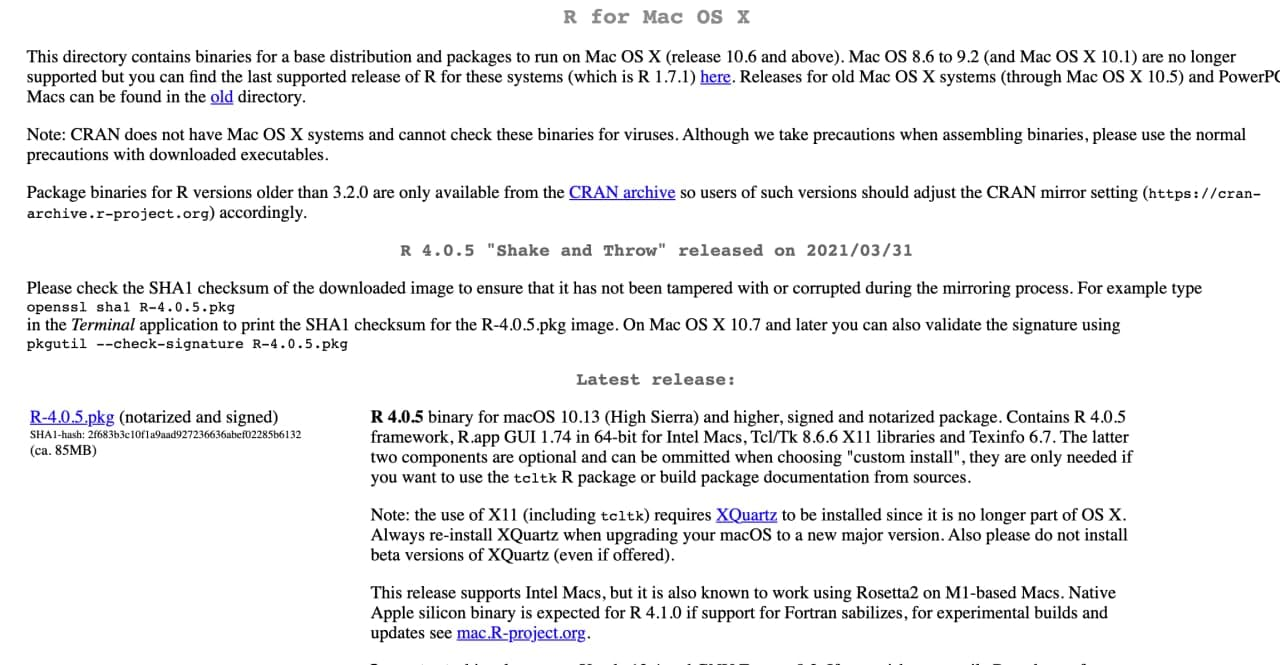
\includegraphics[width=0.6\linewidth]{./img/pantall_mac_cran} 

}

\caption{Pantalla de instalación de R en Mac OS.}\label{fig:pantalla-mac}
\end{figure}

Para sistemas operativos Windows, debemos clickar en \texttt{install\ R\ for\ the\ first\ time} (ver imagen \ref{fig:pantalla-windows-1}) y en la siguiente pantalla hacer click en \texttt{Download\ R\ for\ Windows} (ver imagen \ref{fig:pantalla-windows-2}). Una vez descargado, abrirlo como cualquier archivo.

\begin{figure}

{\centering 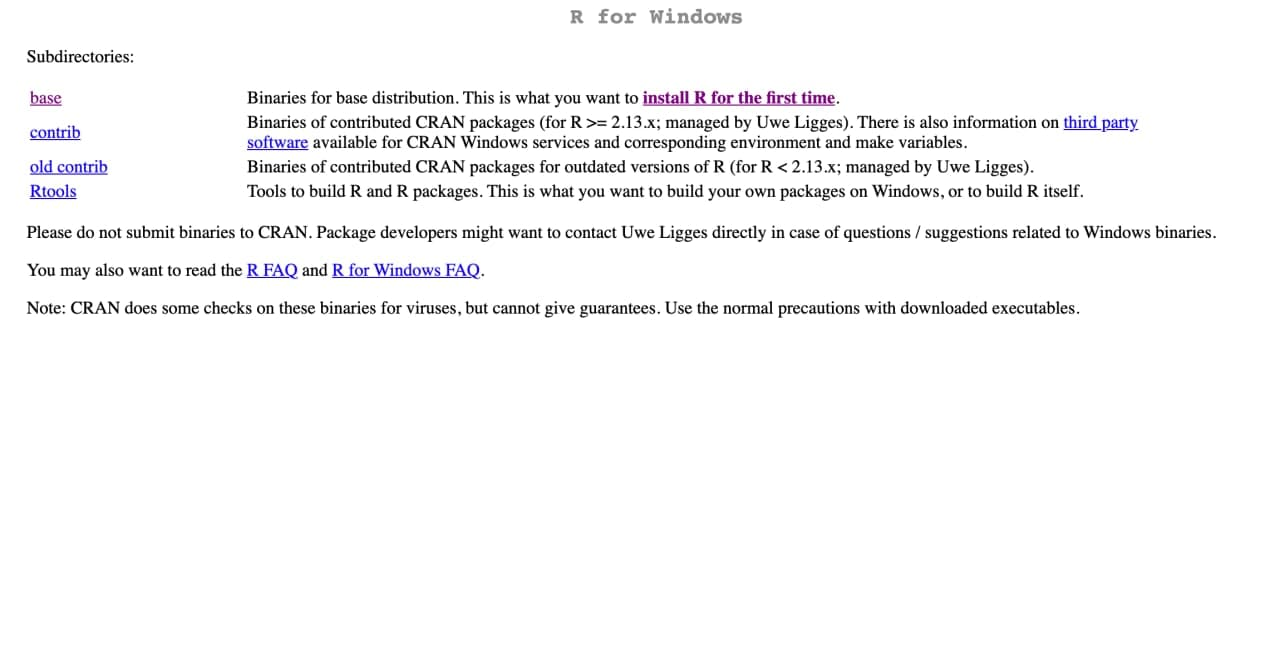
\includegraphics[width=0.6\linewidth]{./img/pantalla_windows_1} 

}

\caption{Pantalla previa de instalación de R en Windows.}\label{fig:pantalla-windows-1}
\end{figure}

\begin{figure}

{\centering 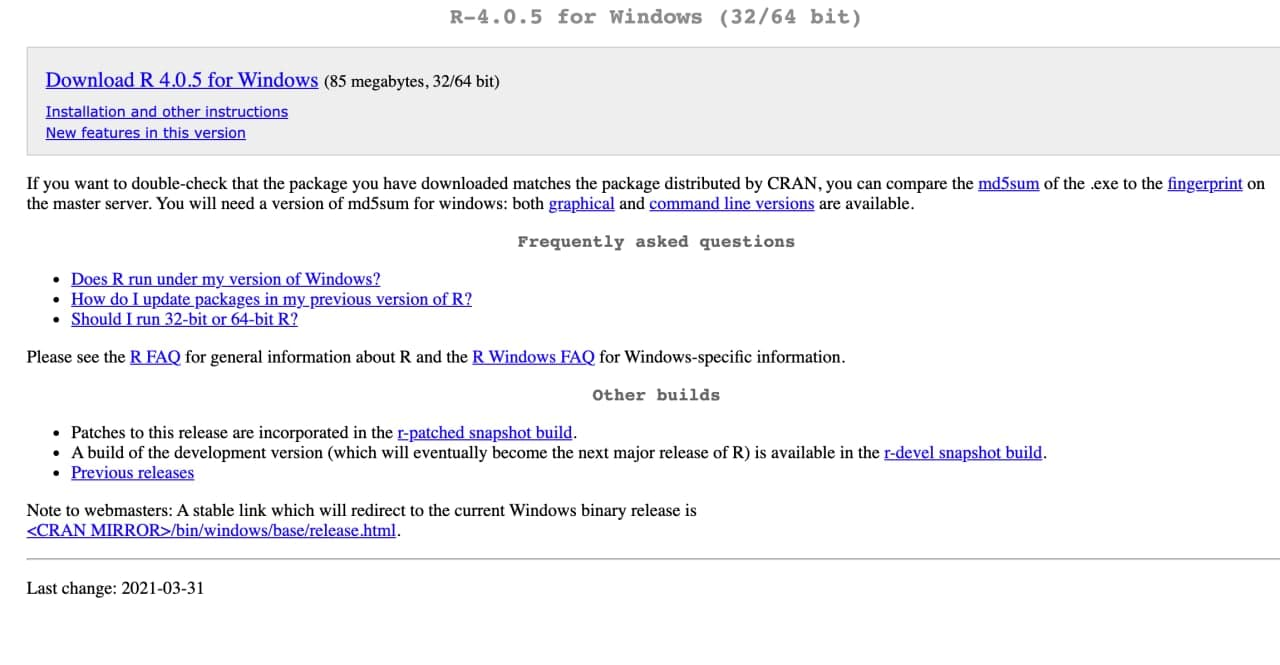
\includegraphics[width=0.75\linewidth]{./img/pantalla_windows_2} 

}

\caption{Pantalla final de instalación de R en Windows.}\label{fig:pantalla-windows-2}
\end{figure}

\begin{itemize}
\tightlist
\item
  \textbf{Paso 3}: tras su instalación tendrás en tu escritorio (Windows) o en tu Launchpad (Mac Os) un \textbf{ejecutable de \texttt{R} para abrir}. En Windows puede que tengas dos ejecutables \texttt{i386} y \texttt{x64} (como todo programa en Windows está la versión de 32 y de 64 bits, haz click preferiblemente - si lo tienes - en el de \texttt{x64}). Te saldrá algo parecido a lo que observas en la imagen \ref{fig:cranR}.
\end{itemize}

\begin{figure}

{\centering 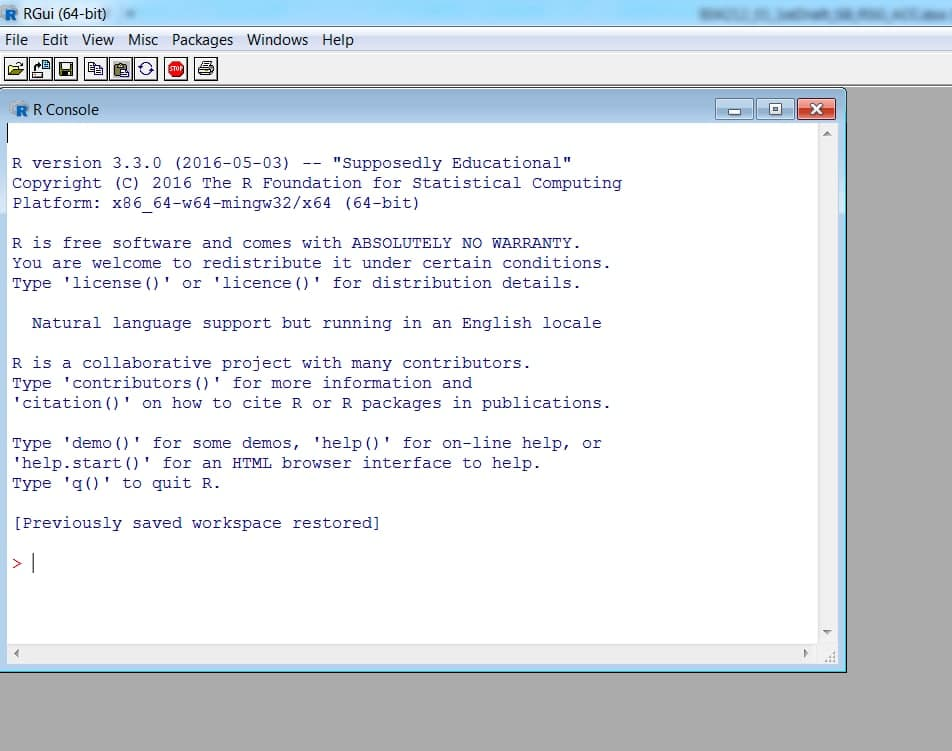
\includegraphics[width=0.75\linewidth]{./img/cranR} 

}

\caption{Primera pantalla al abrir el ejecutable de R.}\label{fig:cranR}
\end{figure}

Para comprobar que está correctamente instalado, \textbf{prueba a escribir en la consola} el siguiente código (\textbf{recuerda}: los códigos puedes copiarlos directamente de la cajita en la que está haciendo click en el botón de la esquina superior derecha)

\begin{Shaded}
\begin{Highlighting}[]
\NormalTok{a <-}\StringTok{ }\DecValTok{1}
\NormalTok{b <-}\StringTok{ }\DecValTok{2}
\NormalTok{a }\OperatorTok{+}\StringTok{ }\NormalTok{b}
\end{Highlighting}
\end{Shaded}

\begin{verbatim}
## [1] 3
\end{verbatim}

\begin{figure}

{\centering 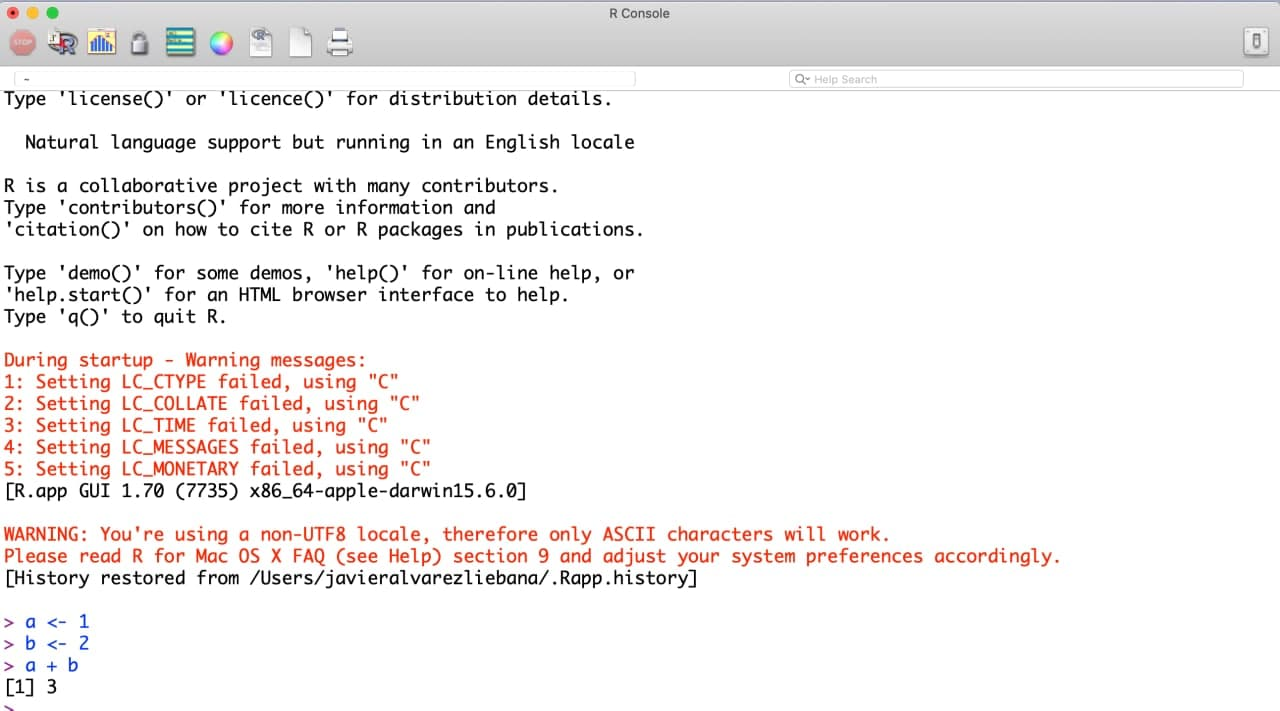
\includegraphics[width=0.75\linewidth]{./img/primera_suma} 

}

\caption{Primera suma en la consola de R.}\label{fig:primera-suma}
\end{figure}

\textbf{¡Enhorabuena!} Si te ha devuelto \texttt{{[}1{]}\ 3}, ya has hecho más de lo que parece: has definido dos variables \texttt{a} y \texttt{b}, has \textbf{asignado un valor numérico a cada variable} y las hemos usado. \textbf{Ya sabemos usar \texttt{R} como calculadora}.

~


\includegraphics[width=0.04\textwidth,height=\textheight]{img/logo_info.png} \textbf{Asignación}: como habrás advertido, en \texttt{R} usaremos \texttt{\textless{}-} para asignar valores en lugar de \texttt{=}, como una flecha.

~


\includegraphics[width=0.04\textwidth,height=\textheight]{img/logo_info.png} \textbf{Línea de consola}: como habrás advertido, en \texttt{R} usaremos \texttt{\textless{}-} para asignar valores en lugar de \texttt{=}, como una flecha.

~

~

Bonita esta interfaz no es, así que la cerraremos y no la abriremos más. Tenemos nuestro lenguaje instalado, vamos a \textbf{instalar nuestro Word} para poder programar de forma cómoda.

\hypertarget{instalacionRStudio}{%
\section{Instalación de RStudio}\label{instalacionRStudio}}

Para instalar \texttt{RStudio} deberemos ir a la web \url{https://www.rstudio.com/products/rstudio/download/\#download} y seleccionar el ejecutable que te aperezca acorde a tu sistema operativo (ver imagen \ref{fig:pantalla-rstudio}). Tras descargar el ejecutable, hay que abrirlo como otro cualquier otro ejecutable y dejar que termine la instalación.

\begin{figure}

{\centering 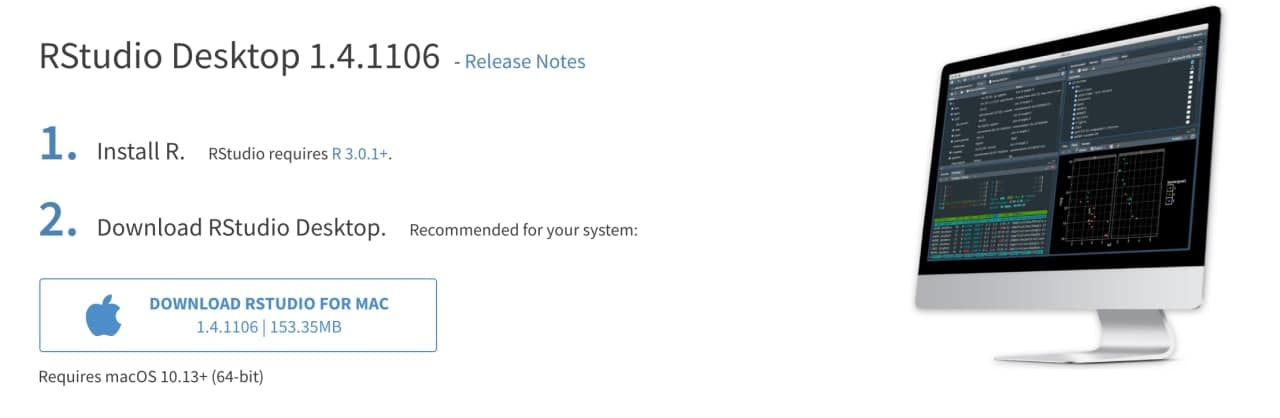
\includegraphics[width=0.75\linewidth]{./img/pantalla_rstudio} 

}

\caption{Descargar el ejecutable de RStudio para su posterior instalación.}\label{fig:pantalla-rstudio}
\end{figure}

Tras instalar tendremos en el escritorio o Launchpad un ejecutable de \texttt{RStudio} que abriremos. Se nos aparecerá una pantalla similar a esta:

\begin{figure}

{\centering 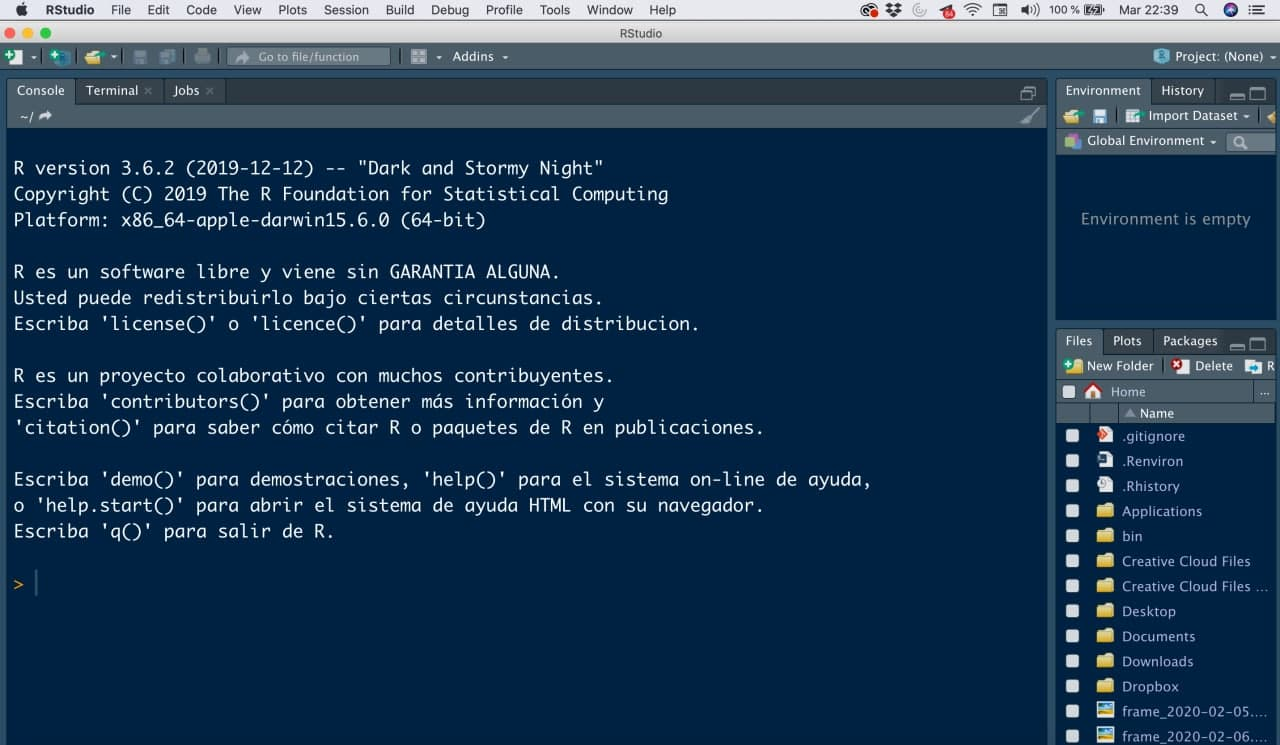
\includegraphics[width=0.75\linewidth]{./img/inicio_rstudio_1} 

}

\caption{Primer recibimiento de nuestro mejor amigo RStudio.}\label{fig:inicio-rstudio-1}
\end{figure}

\begin{itemize}
\tightlist
\item
  \textbf{Consola}: es el nombre para llamar a esa ventana grande que te ocupa la mayor parte de tu pantalla. Prueba a escribir el mismo código que antes en ella (es el equivalente a la consola de R que hemos abierto al principio).
\end{itemize}

\begin{Shaded}
\begin{Highlighting}[]
\NormalTok{a <-}\StringTok{ }\DecValTok{1}
\NormalTok{b <-}\StringTok{ }\DecValTok{2}
\NormalTok{a }\OperatorTok{+}\StringTok{ }\NormalTok{b}
\end{Highlighting}
\end{Shaded}

\begin{figure}

{\centering 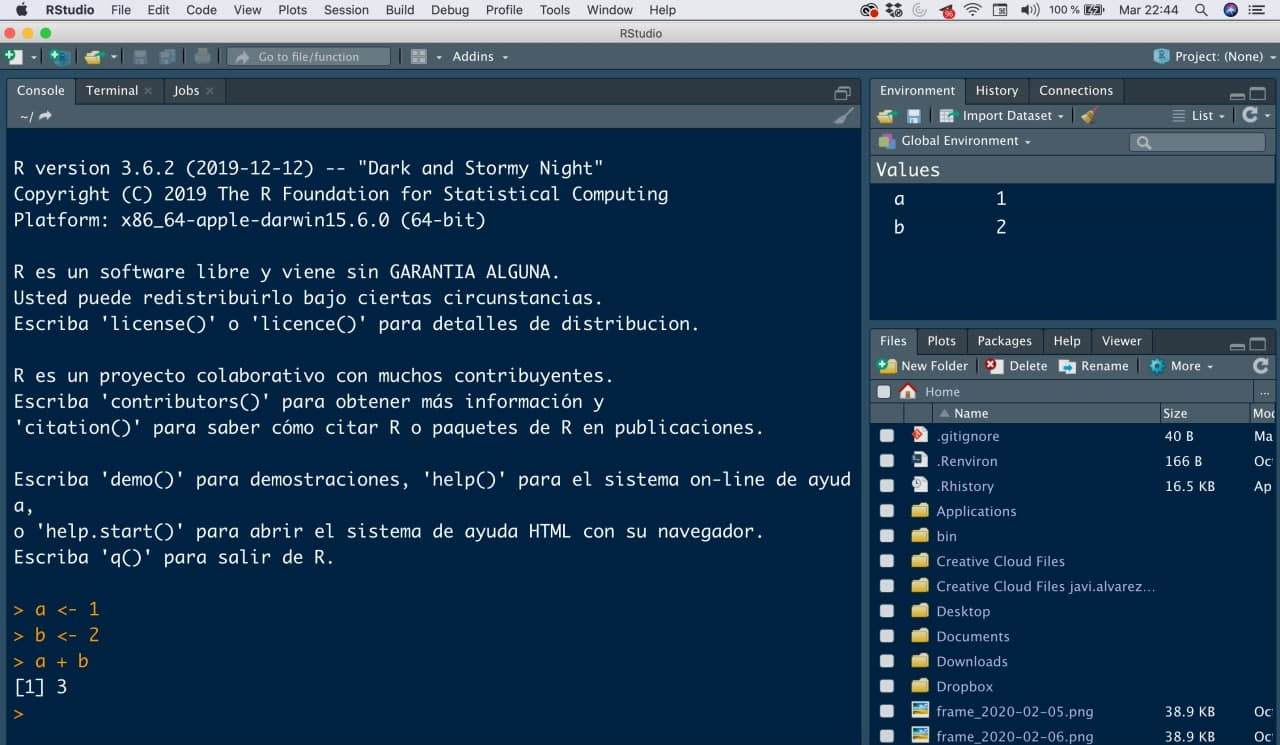
\includegraphics[width=0.75\linewidth]{./img/inicio_rstudio_2} 

}

\caption{Lanzando a consola nuestras primeras órdenes en RStudio.}\label{fig:inicio-rstudio-2}
\end{figure}

\textbf{La consola será donde ejecutaremos órdenes y mostraremos resultados}

\begin{itemize}
\tightlist
\item
  \textbf{Environment (entorno)}: la pantalla pequeña (puedes ajustar los márgenes con el ratón a tu gusto) que tenemos en la parte superior derecha se denomina environment o entorno de variables, donde como puedes ver, tras ejecutar el pequeño código en la consola, nos informa de que tenemos dos variables numéricas y su valor asignado. Nos \textbf{mostrará las variables que tenemos definidas, el tipo y su valor}.
\end{itemize}

\begin{figure}

{\centering 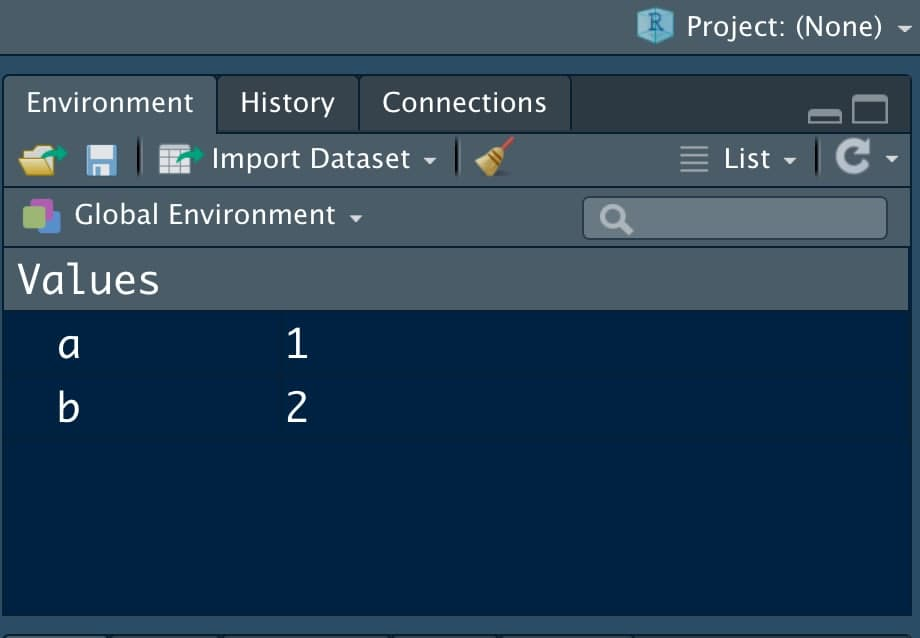
\includegraphics[width=0.75\linewidth]{./img/inicio_rstudio_3} 

}

\caption{Environment de variables.}\label{fig:inicio-rstudio-3}
\end{figure}

\begin{itemize}
\tightlist
\item
  \textbf{Panel multiusos}: la ventana que tenemos en la parte inferior derecha no servirá para buscar ayuda de comandos y órdenes, además de para visualizar gráficos. Lo veremos cuando sea necesario.
\end{itemize}

\begin{figure}

{\centering 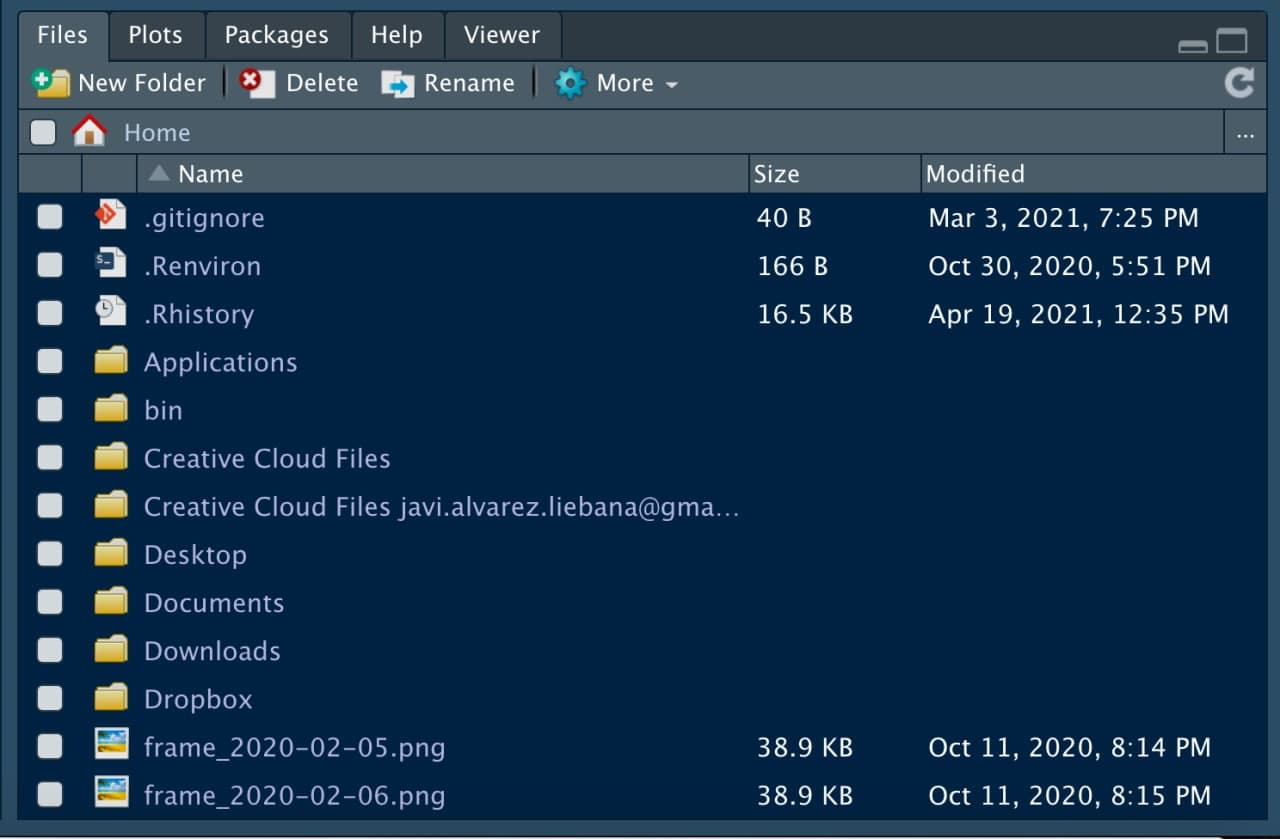
\includegraphics[width=0.75\linewidth]{./img/inicio_rstudio_4} 

}

\caption{Panel multiusos.}\label{fig:inicio-rstudio-4}
\end{figure}

\textbf{WTF ¿Y DÓNDE PROGRAMAMOS?}

\textbf{¿Estás emocionado/a? Vamos a abrir nuestro primer script} (script = documento en el que programamos, nuestro \texttt{.doc}, pero aquí será un archivo \texttt{.R}).

Haz click en el menú superior en \texttt{File\ \textless{}\textless{}\ New\ File\ \textless{}\textless{}\ R\ Script} como se muestra en la imagen \ref{fig:inicio-rstudio-5}

\begin{figure}

{\centering 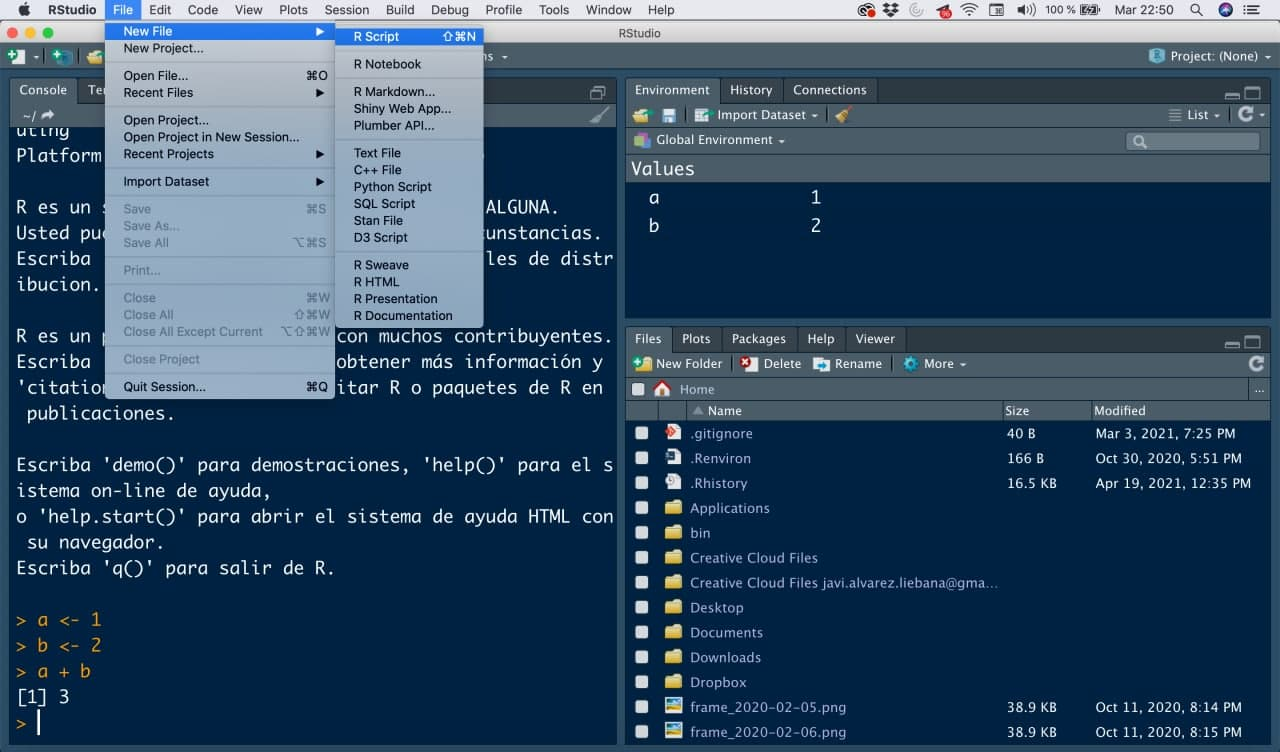
\includegraphics[width=0.75\linewidth]{./img/inicio_rstudio_5} 

}

\caption{Abriendo nuestro primer script de R.}\label{fig:inicio-rstudio-5}
\end{figure}

Tras abrirlo tendremos una cuarta ventana: esta será la ventana de nuestros códigos, la ventana más importante ya que es donde \textbf{escribiremos lo que queremos ejecutar}. Escribe el código de arriba en ese script y guarda el archivo haciendo click en el botón \texttt{Save\ current\ document}

\begin{figure}

{\centering 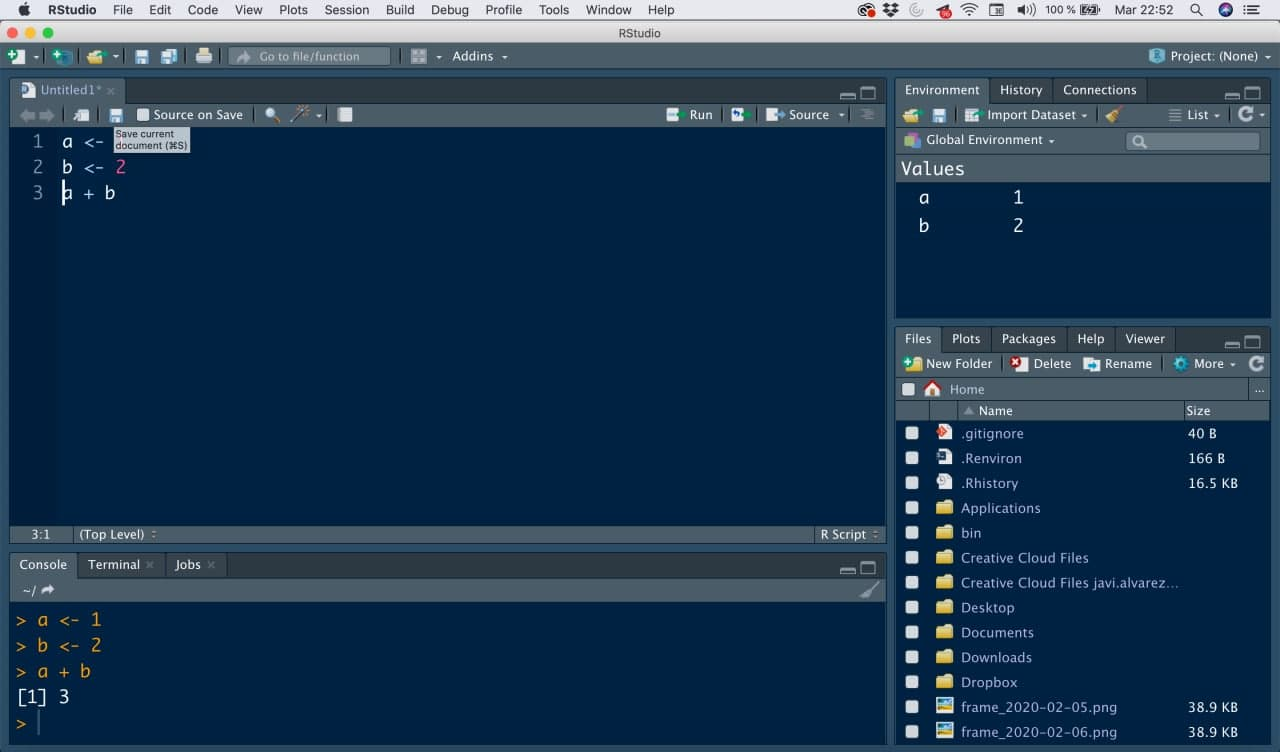
\includegraphics[width=0.75\linewidth]{./img/inicio_rstudio_6} 

}

\caption{Escribiendo y guardando nuestro primer script.}\label{fig:inicio-rstudio-6}
\end{figure}

Ese código no se ejecuta salvo que se lo digamos. Tenemos dos opciones para ello: o copiamos el trozo de código que queramos y lo pegamos en la consola (como hemos hecho al principio), o \textbf{activamos el cuadrado \texttt{Source\ on\ save} a la derecha del botón de guardar} y volvemos a hacer click en el botón de guardar: siempre que esa opción esté activada, al guardar no solo es nos guarda el archivo \texttt{.R} sino que además se ejecuta solo y nos devuelve los resultados por consola.

Listo, tienes instalado (casi) todo correctamente.

\hypertarget{instalacionpaquetes}{%
\section{Instalación de paquetes}\label{instalacionpaquetes}}

El lenguaje \texttt{R} tiene 3 ventajas principales:

\begin{itemize}
\item
  Es un \textbf{lenguaje creado por y para estadísticos/as}, por lo que está pensado para optimizar al máximo los recursos, y poder hacer un análisis estadístico de calidad
\item
  Es \textbf{software libre} (como C, C++, Python, Fortran, y otros tantos lenguajes). El software libre no solo tiene una ventaja evidente (es gratis, ok) en su instalación sino que permite acceder al código en el que están programados los comandos y permite hacer uso de trozos de código de otras personas.
\item
  Es un \textbf{lenguaje modular}: en la instalación no se instalan todas las funcionalidades sino que instala un mínimo para poder funcionar, de forma que se ahorra espacio en disco y en memoria. Al ser software libre, existen trozos de código hechos por otras personas llamados \textbf{paquetes}, que podemos ir instalando a nuestro gusto según los vayamos necesitando. Esto es una ventaja enorme ya que \texttt{R} tiene una comunidad de usuarios gigante, con \textbf{más de 17 000 paquetes}: ¡hay más de 17 000 trozos de código validados por la comunidad y la plataforma, de forma gratuita!
\end{itemize}

\begin{figure}

{\centering 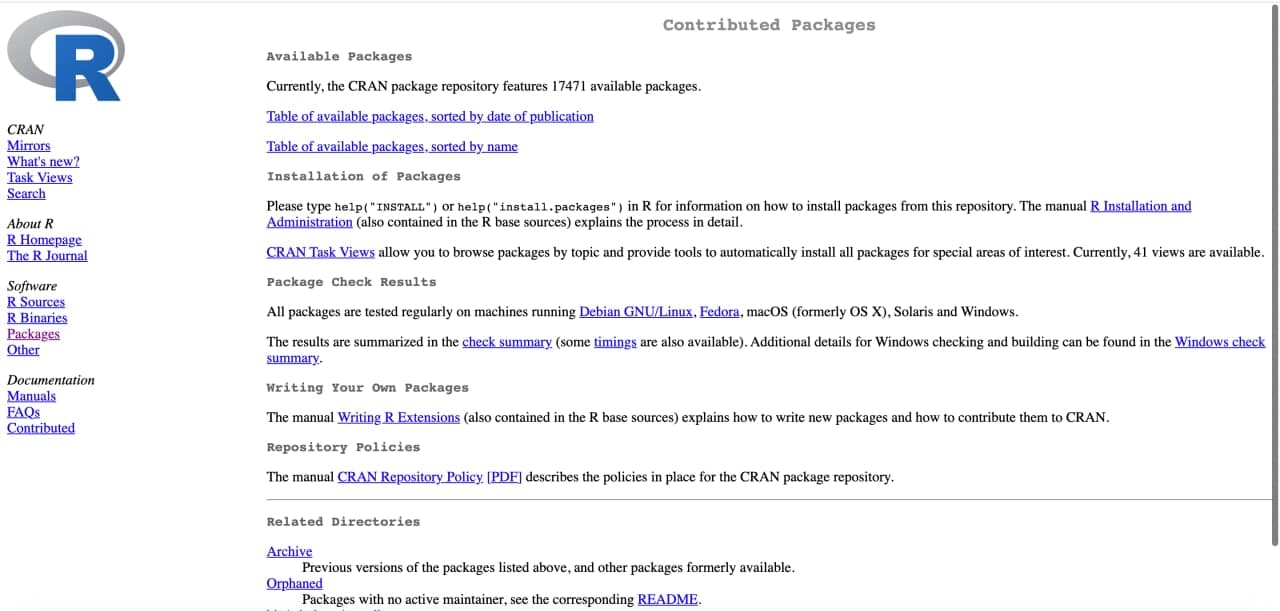
\includegraphics[width=0.75\linewidth]{./img/paquetes_R} 

}

\caption{Paquetes disponibles en R.}\label{fig:paquetes-R}
\end{figure}

Esto nos ahorra muchísimo tiempo ya el \textbf{90\% de lo que querramos hacer ya lo habrá querido hacer otra persona y podemos usar o adaptar su código} para no empezar de cero. Vamos a instalar un paquete gráfico (\texttt{\{ggplot2\}}) que necesitaremos. Para ello, escribe en tu consola el siguiente código y pulsa enter.

\begin{Shaded}
\begin{Highlighting}[]
\KeywordTok{install.packages}\NormalTok{(}\StringTok{"ggplot2"}\NormalTok{)}
\end{Highlighting}
\end{Shaded}

Dicha orden (puede tardar un poco la primera vez, depende de tu conexión a internet) lo que hará será acceder a la web de R, bajarse a tu ordenador los trozos de código incluidos en el paquete llamado \texttt{\{ggplot2\}} (para realizar gráficas), y dejarlos para siempre en él: \textbf{la instalación de paquetes SOLO ES NECESARIO la primera vez} que se usa dicho paquete en la vida del ordenador, no hace falta hacerlo cada vez que lo usas.

Una vez que tenemos los trozos de código (el paquete) en nuestro ordenador, en cada sesión de \texttt{R} que abramos (cada vez que cierres y abras \texttt{RStudio}) deberemos (si queremos) llamar a ese paquete que tenemos instalado, escribiendo el siguiente comando en consola

\begin{Shaded}
\begin{Highlighting}[]
\KeywordTok{library}\NormalTok{(ggplot2)}
\end{Highlighting}
\end{Shaded}

\textbf{Welcome to software libre}

\hypertarget{consejos-y-tips}{%
\section[ Consejos y tips]{\texorpdfstring{\protect
\includegraphics[width=0.04\textwidth,height=\textheight]{img/logo_info.png} Consejos y tips}{ Consejos y tips}}\label{consejos-y-tips}}

¿Cómo saber cuando la orden lanzada en consola ha terminado?

A veces \texttt{R} y \texttt{RStudio} son tan silenciosos que no sabemos si ha acabado la orden que acabamos de lanzar en la consola o no.


\includegraphics[width=0.04\textwidth,height=\textheight]{img/logo_info.png} \textbf{Truco}: siempre que veas este símbolo \texttt{\textgreater{}} como última línea en la consola significa que está listo para que le escribamos otra orden (es la forma cariñosa de decirte que ya ha acabado, ver imagen \ref{fig:tip-consola-lista})

\begin{figure}

{\centering 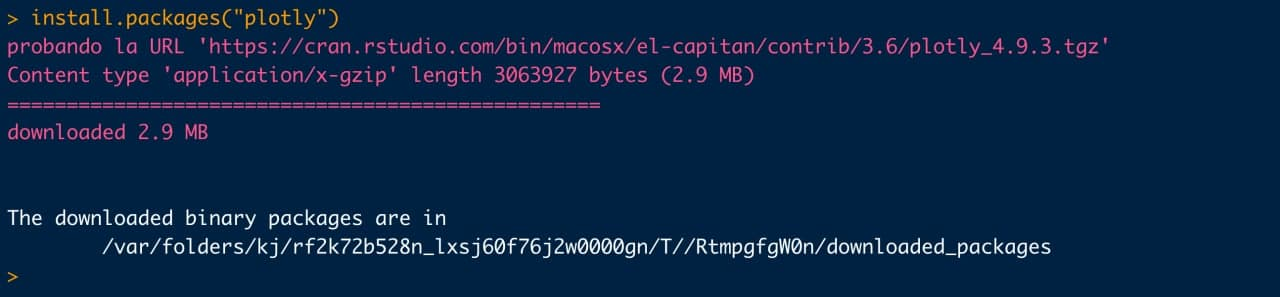
\includegraphics[width=0.7\linewidth]{./img/tip_consola_lista} 

}

\caption{Ejemplo de que la orden lanzada ha acabado.}\label{fig:tip-consola-lista}
\end{figure}

~

¿Cómo prevenir la fatiga visual programando?

Estar delante de una pantalla de ordenador, con la vista muy fija mientras se programa, puede que acabes teniendo cierta fatiga visual en el trabajo.


\includegraphics[width=0.04\textwidth,height=\textheight]{img/logo_info.png} \textbf{Truco}: te aconsejo que cambies en tu \texttt{RStudio} la tonalidad del fondo de tu programa, en tonos oscuros y no blancos (¿te has fijado que mis capturas tienen un azul cobalto oscuro de fondo mientras el tuyo es un blanco nuclear? Echa un vistazo las imagenes \ref{fig:menu-1} y \ref{fig:menu-2})

\begin{figure}

{\centering 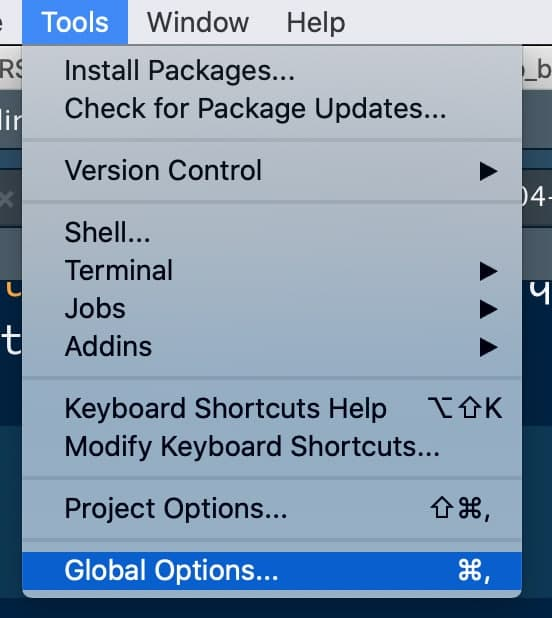
\includegraphics[width=0.4\linewidth,height=0.4\textheight]{./img/menu_1} 

}

\caption{Menú de opciones de nuestro editor}\label{fig:menu-1}
\end{figure}

\begin{figure}

{\centering 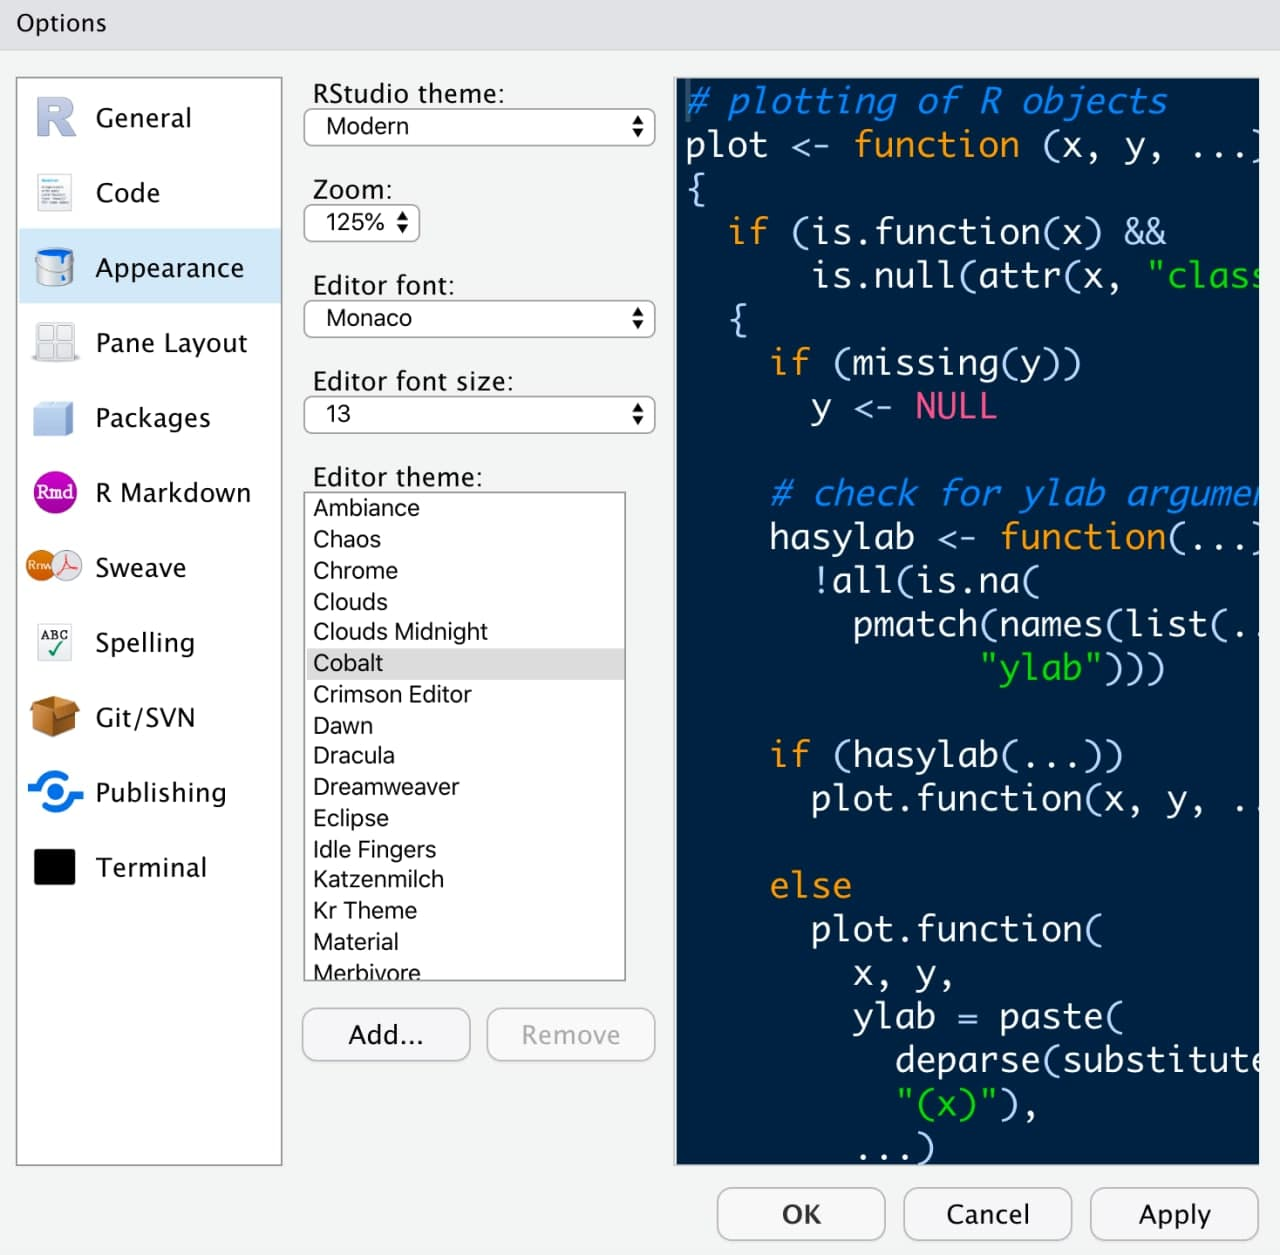
\includegraphics[width=0.4\linewidth,height=0.4\textheight]{./img/menu_2} 

}

\caption{Personalizar el color de fondo de nuestro editor, la letra y el tamaño de fuente}\label{fig:menu-2}
\end{figure}

~

Entender los paquetes

Haciendo una metáfora con la colección de libros que tengas en casa: con la \textbf{instalación hemos comprado el libro} y lo tenemos en nuestra estantería (para siempre), con la llamada al paquete, por ejemplo \texttt{library(ggplot2)}, lo que hacemos es decidir, de entre todos los libros de la estantería, cuales queremos llevarnos de viaje (en cada maleta que hagamos).

Los \textbf{paquetes usados} los verás denotados como \texttt{\{nombre\_paquete\}} a lo largo del manual.

\hypertarget{primeros-pasos}{%
\chapter{Primeros pasos}\label{primeros-pasos}}

\textbf{¿Empezamos?}

Veamos antes \textbf{un poco de historia} sobre nuestro deidad.

Allá por 1975, los \textbf{laboratorios Bell} (los que inventaron la radio moderna tal y como la conocemos), necesitaban una alternativa a los lenguajes más «rudos» y antiguos como \texttt{C++} o \texttt{Fortran}, lenguajes rápidos en la ejecución pero complejos en su uso, con una gran curva de aprendizaje y con \textbf{muy poca capacidad en la visualización de datos} que se empezaba a necesitar.

Así que en \textbf{1976 sacaron la primera versión del lenguaje conocido \texttt{S}} (hasta entonces estaba de moda lo de llamar a los lenguajes con una sola inicial). En \textbf{1980} se empezó a distribuir la primera versión pública de \texttt{S}, más allá de los laboratorios Bell, y en \textbf{1988} se añadieron bastantes funcionalidades nuevas como poder aplicar funciones a otras funciones (los famosos \texttt{apply()} que ya veremos). Años más tarde, en \textbf{1991}, dicho lenguaje se simplificó, reescribiendo muchas subrutinas de otros lenguajes más primitivos, para tener una versión muy parecida al actual \texttt{R}, permitiendo el usod de operadores, \texttt{data.frames} (que veremos) y otro tipo de objetos, sencillos en la programación pero muy versatiles.

Sin embargo, salvo uso docente, \texttt{S} tenía licencia así que \textbf{en 1992 Ross Ihaka y Robert Gentleman se lanzaron a crear una versión de \texttt{S} libre y gratuita}, un trabajo de casi 8 años hasta que en el año 2000, ambos investigadores de la Universidad de Auckland en Nueva Zelanda lanzaron la primera versión estable del lenguaje.

Tras dicho lanzamiento, se creó un \textbf{equipo de expertos en estadística computacional (el conocido como \emph{R Development Core Team})} que es el que se encarga de mantener toda la aerquitectura de \texttt{R} y los que se encargar de actualizar y mejorar el paquete \texttt{\{base\}}, una \textbf{librería motor} sobre la que se construye el resto de funciones.

\hypertarget{excel-no-es-tu-amigo}{%
\section{Excel no es tu amigo}\label{excel-no-es-tu-amigo}}

\textbf{\texttt{R} es un lenguaje de programación}, de alto nivel para el usuario y modular. Los lenguajes de alto nivel como \texttt{R}, \texttt{Python} (curso interactivo de Python en \url{https://checkio.org/}) o \texttt{Matlab}, facilitan la programación al usuario, teniendo que preocuparte solo de la tarea de programar. Son lenguajes con una \textbf{menor curva de aprendizaje} aunque suelen ser más lentos en su ejecución en comparación con lenguajes de bajo nivel (\texttt{C}, \texttt{C++} o \texttt{Fortran}), lenguajes muy rápidos en su ejecución pero cuya programación requiere un mayor tiempo y formación, teniendo que además estar pendiente del tipo de variables, espacio en memoria, etc.

Por su arquitectura, \texttt{R} es un lenguaje que puede ser usado para un propósito general pero que está especialmente diseñado para el \textbf{análisis estadístico de datos}. Su \textbf{modularidad} nos da la ventaja de que podemos instalar las funcionalidades que vayamos necesitando de forma progresiva.

\textbf{¿Por qué no es recomendable usar Excel?}

\begin{itemize}
\item
  \textbf{Software de pago}: Excel, al igual que el resto de programas de Microsoft o SPSS (por desgracia programa estrella de nuestro sistema sanitario), es un programa de pago. A nivel individual, todos hemos tenido una versión que no hemos pagado, pero dicha evasión no se la puede permitir una empresa o administración, que debe de pagar altas cantidades de dinero anuales por las licencias, dinero que no sería necesario si los investigadores y trabajadores tuvieran formación (remunerada) en otras herramientas de software libre.
\item
  \textbf{Software cerrado}: no solo es de pago sino que es cerrado, así que solo podemos hacer lo que Excel ha creído que interesante que podamos hacer. Incluso con la programación de MACROS, las funcionalidades de Excel siguen siendo mucho más limitadas ya que viene «programadas» de antemano
\item
  \textbf{Alto consumo de memoria}: dicha programación predeterminada hace que Excel ocupe muchísimo espacio en el disco duro y tenga un alto consumo de memoria (la memoria es lo que te permite hacer varias tareas a la vez en tu ordenador).
\item
  \textbf{No es universal}: no solo es de pago sino que además, dependiendo de la versión que tengas de Excel, tendrá un formato distinto para datos como fechas, teniendo incluso extensiones distintas, de forma que un archivo \texttt{.xls} abierto por un Excel moderno puede provocar errores en la carga.
\item
  \textbf{¡ES SOLO UNA HOJA DE CÁLCULO!}: el propio Microsoft desaconseja el uso de Excel para el análisis de grandes volúmenes de datos. El Excel es una herramienta maravillosa para ser usada como una sencilla hoja de cálculo: llevar las cuentas de tu familia, de tu pequeño negocio, una declaración de la Renta sencilla, planificar viajes, etc. Pero el programa \textbf{NO ESTÁ DISEÑADO} para ser una base de datos ni para análisis detallado, y muchos menos pensado para generar un entorno flexible para el análisis estadístico y la visualización de datos.
\end{itemize}

\textbf{¿Puedes ser el mejor partiendo un filete con una cuchara?} Seguramente puedas (en Excel puedes hasta programar con macros), y si siempre lo hiciste así, acabarás normalizándolo, pero seguirás siendo una persona comiendo filete con cuchara.

~


\includegraphics{img/pregunta.png} \textbf{¿Qué sucede si usamos la herramienta equivocada?}

Tres ejemplos:

\begin{itemize}
\tightlist
\item
  \textbf{Problemas para codificar fechas}: en 2016 se publicó una \href{https://genomebiology.biomedcentral.com/articles/10.1186/s13059-016-1044-7}{revisión de artículos en genética}, descubriendo que 1 de cada 5 artículos contenían errores debido a una mala codificación de las fechas, conviertiendo por ejemplo los genes Septin-2 (conocido como SEPT2) en fechas, y al revés \citep{Ziemannetal16}.
\end{itemize}

\begin{figure}

{\centering 
\includegraphics[width=0.5\linewidth]{./img/excel_genes} 

}

\caption{Excel en una noche loca.}\label{fig:excel-genes}
\end{figure}

\begin{itemize}
\tightlist
\item
  \textbf{Problemas de memoria}: un Excel permite por defecto una cantidad máxima de filas. Aunque dicha cantidad se puede ampliar, sigue siendo finita, por lo que cuando superas el umbral de filas, al añadir filas Excel te borra registros \textbf{sin avisarte de que lo está haciendo}. Esto es lo que sucedió con los \href{https://www.redaccionmedica.com/secciones/sanidad-hoy/covid-reino-unido-pierden-16000-positivos-9989}{registros de casos covid en Reino Unido}.
\end{itemize}

\begin{figure}

{\centering 
\includegraphics[width=0.5\linewidth]{./img/excel_uk} 

}

\caption{Cuando Excel dice basta.}\label{fig:excel-uk}
\end{figure}

\begin{itemize}
\tightlist
\item
  \textbf{Problemas para codificar edades}: una variable de tipo fecha, aunque nosotros la veamos con letras, en realidad es una variable numérica que representa los días que han pasado desde una fecha origen. En función de las distintas versiones de Excel, dicha fecha origen cambia. Además, si se codifica mal la fecha en formato \texttt{dd-mm-YY}, dicho formato cuando se exporta a otro excel en texto, no permite distinguir a un nacido en 1918 y a un nacido en 2018, así que podemos estar confundiendo personas de 103 años con niños de 3 años (y es lo que \href{https://www.niusdiario.es/sociedad/sanidad/sanidad-reconoce-datos-muertes-ninos-covid-erroneos-contabilizaban-centenarios-como-menores_18_3107220241.html}{sucedió en España}, observando unas tasas de mortalidad en niños muy pequeños equivalentes a personas mayores).
\end{itemize}

\begin{figure}

{\centering 
\includegraphics[width=0.5\linewidth]{./img/excel_edades} 

}

\caption{Los centenarios con biberón.}\label{fig:excel-edades}
\end{figure}

\hypertarget{primeros-pasos-calculadora}{%
\section{Primeros pasos: calculadora}\label{primeros-pasos-calculadora}}

¿Te acuerdas de lo que era la \textbf{consola}? Vamos a trabajar de momento en esa ventana que tienes en la ventana inferior.

\begin{figure}

{\centering 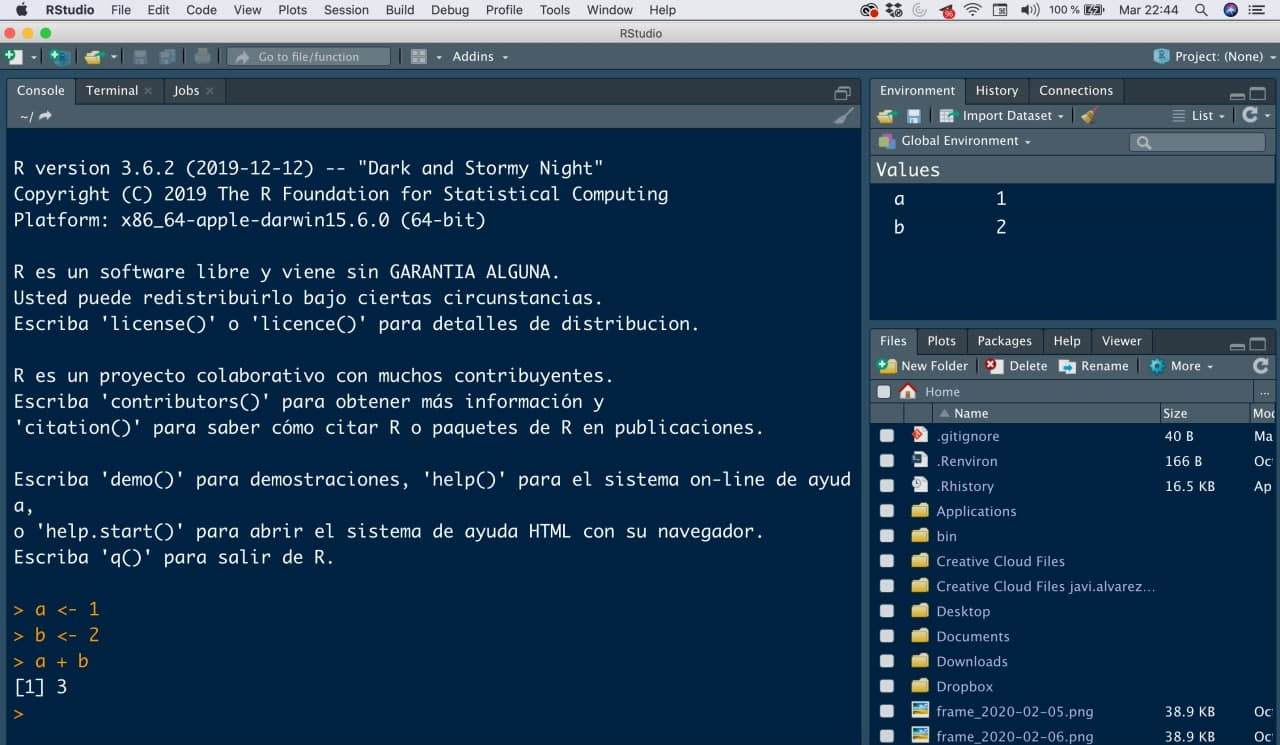
\includegraphics[width=0.75\linewidth]{./img/inicio_rstudio_2} 

}

\caption{Lanzando a consola nuestras primeras órdenes en RStudio.}\label{fig:inicio-rstudio-2a}
\end{figure}

Lo que ya hemos descubierto en los pasos de la instalación (ver imagen \ref{fig:inicio-rstudio-2a}) es que la consola de \texttt{R} tiene una función muy básica y evidente: nos sirve de calculadora. Un ejemplo muy simple: si escribimos 3 en la consola y pulsamos \emph{ENTER}, la consola nos mostrará el resultado de la suma

\begin{Shaded}
\begin{Highlighting}[]
\DecValTok{1} \OperatorTok{+}\StringTok{ }\DecValTok{2}
\end{Highlighting}
\end{Shaded}

\begin{verbatim}
## [1] 3
\end{verbatim}

~

\textbf{¿Pero cuál es la diferencia entre una calculadora y un lenguaje de programación?}

Imagina que dicha suma 3 la quisiéramos utilizar para un segundo cálculo: ¿y si en lugar de lanzarlo a la consola sin más lo \textbf{almacenamos en alguna variable}?

Como hemos visto en la instalación de \texttt{RStudio}, para \textbf{asignar variables} lo haremos con la orden \texttt{x\ \textless{}-\ 1\ +\ 2}: una variable de nombre \texttt{x} va a tener asignada \texttt{\textless{}-} lo que valga la suma \texttt{1\ +\ 2}

\begin{Shaded}
\begin{Highlighting}[]
\NormalTok{x <-}\StringTok{ }\DecValTok{1} \OperatorTok{+}\StringTok{ }\DecValTok{2}
\end{Highlighting}
\end{Shaded}

Como puedes comprobar, en tu parte superior derecha (nuestro entorno de variables), podrás ver como una nueva variable \texttt{x} es ahora visualizada, con su valor asignado (\textbf{no se mostrará en consola} salvo que escribas 3 en ella: \texttt{R} asume que no querías visualizarla en consola sino solo guardarla).

\begin{figure}

{\centering 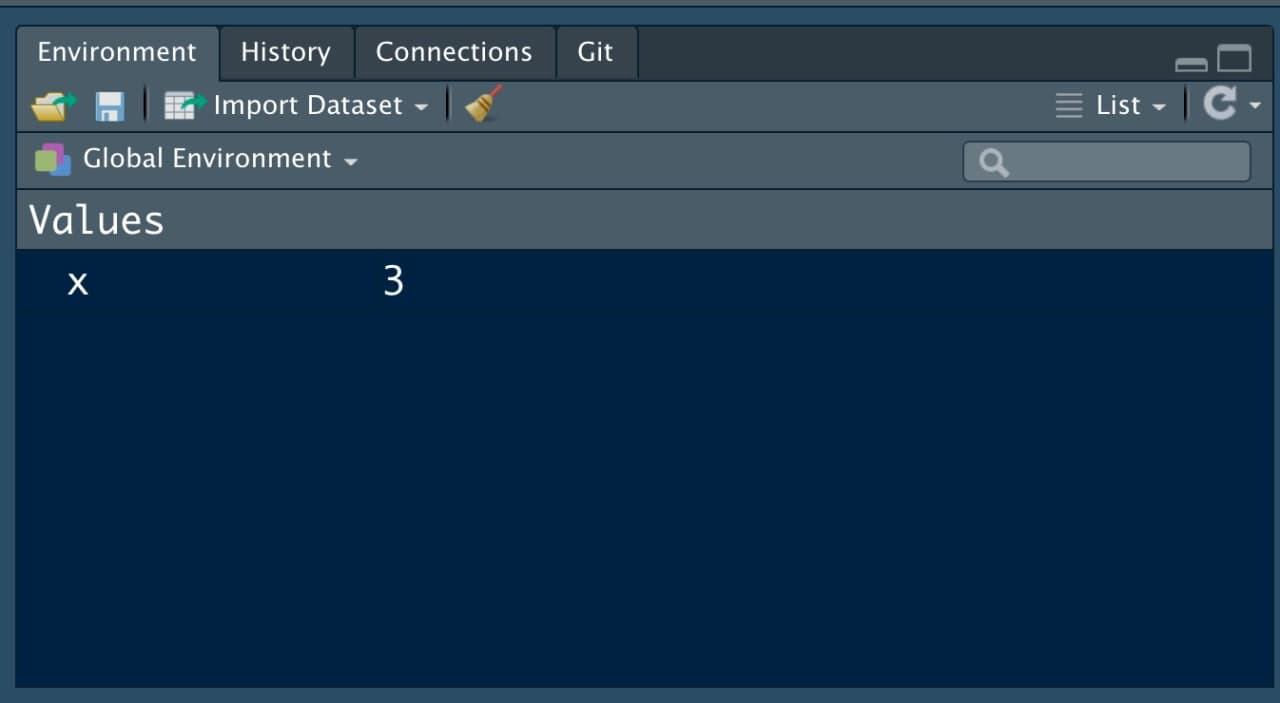
\includegraphics[width=0.75\linewidth]{./img/environment_1} 

}

\caption{Environment.}\label{fig:unnamed-chunk-4}
\end{figure}

Dicha variable \texttt{x} además podemos reciclarla para definir una variable \texttt{y}, restándole una constante.

~

De la misma manera que hemos hecho restas, sumas y multiplicaciones, \texttt{R} tiene todas las operaciones clásicas que podrías tener en una calculadora. Prueba a ejecutar en la consola las órdenes \texttt{x\^{}2}, \texttt{sqrt(x)} o \texttt{abs(y)}: \texttt{R} calculará las operaciones \emph{elevar al cuadrado}, \emph{raíz cuadrada} y \emph{valor absoluto} de la variable que tengan entre paréntesis

\begin{Shaded}
\begin{Highlighting}[]
\NormalTok{x}\OperatorTok{^}\DecValTok{2}
\end{Highlighting}
\end{Shaded}

\begin{verbatim}
## [1] 9
\end{verbatim}

\begin{Shaded}
\begin{Highlighting}[]
\KeywordTok{sqrt}\NormalTok{(x)}
\end{Highlighting}
\end{Shaded}

\begin{verbatim}
## [1] 1.732051
\end{verbatim}

\begin{Shaded}
\begin{Highlighting}[]
\NormalTok{y <-}\StringTok{ }\NormalTok{x }\OperatorTok{-}\StringTok{ }\DecValTok{5}
\KeywordTok{abs}\NormalTok{(y)}
\end{Highlighting}
\end{Shaded}

\begin{verbatim}
## [1] 2
\end{verbatim}

~

\hypertarget{tipos_errores}{%
\section{Tipos de errores}\label{tipos_errores}}

Durante tu aprendizaje en \texttt{R} va a ser \textbf{muy habitual} que las cosas no salgan a la primera, \textbf{apareciendo en consola mensajes en un color rojo}. Un \textbf{miedo} muy habitual cuando se empieza a programar es pensar que si haces algo mal o aparece algún mensaje de error, el ordenador puede explotar en cualquier momento. \textbf{A programar se aprende programando}, así que haz las pruebas que quieres, lo peor que puede pasar es que necesites cerrar sesión en \texttt{R\ Studio} y abrirlo de nuevo.

Dado que el 99.99999\% de veces tu código tendrá errores que deberás ir solventando, no está de más conocer los tipos de mensajes que \texttt{R} puede sacarte por consola:

\begin{itemize}
\tightlist
\item
  \textbf{\textcolor{red}{Errores}}: los mensajes de error irán precedidos de la frase \textbf{«Error in\ldots{}»}, dándote a veces incluso el tipo de error y la línea de código en la que se ha producido. Veamos un ejemplo intentando sumar un número a una cadena de texto.
\end{itemize}

\begin{Shaded}
\begin{Highlighting}[]
\StringTok{"a"} \OperatorTok{+}\StringTok{ }\DecValTok{1}
\end{Highlighting}
\end{Shaded}

\begin{verbatim}
## Error in "a" + 1: argumento no-numérico para operador binario
\end{verbatim}

Los \textbf{errores son aquellos fallos que seguramente impidan la ejecución} del código. Un \textbf{error muy habitual} es intentar acceder a alguna función de algún paquete que, o bien no tenemos instalado, o bien no hemos llamado haciendo uso del \texttt{library()}: estás intentando leerte un libro de tu biblioteca pero ni siquiera has ido a la tienda a «comprarlo».

\begin{itemize}
\tightlist
\item
  \textbf{\textcolor{yellow}{Warnings}}: los mensajes de \emph{warning} irán precedidos de la frase \textbf{«Warning:\ldots{}»}, y son los fallos más delicados ya que son \textbf{posibles errores o incoherencias} que \texttt{R} detecta en tu código pero que \textbf{no van a hacer que tu código deje de ejecutarse}, aunque probablemente no lo haga como a ti te gustaría. Un ejemplo es cuando tratamos de hacer la raiz cuadrada de un número negativo.
\end{itemize}

\begin{Shaded}
\begin{Highlighting}[]
\KeywordTok{sqrt}\NormalTok{(}\OperatorTok{-}\DecValTok{1}\NormalTok{)}
\end{Highlighting}
\end{Shaded}

\begin{verbatim}
## Warning in sqrt(-1): Se han producido NaNs
\end{verbatim}

\begin{verbatim}
## [1] NaN
\end{verbatim}

¿Ha ejecutado la orden? Sí, pero te **advierte de que el resultado de la operación es un \texttt{NaN}, un valor que no existe (al menos dentro de los números reales), un \emph{Not A Number} (ver Sección \ref{ausentes}).

\begin{itemize}
\tightlist
\item
  \textbf{\textcolor{green}{Mensajes de control}}: los mensajes de control serán aquellos que aparecerán por consola sin empezar por «Error in\ldots{}» ni «Warning:\ldots{}». Dichos mensajes, que puedes incluir tú mismo en tu código con funciones como \texttt{cat()} para monitorizar la ejecución de códigos largos, no son errores ni problemas, son simplemente información que \texttt{R} considera útil aportarte.
\end{itemize}

\hypertarget{consejos-y-tips-1}{%
\section[ Consejos y tips]{\texorpdfstring{\protect
\includegraphics[width=0.04\textwidth,height=\textheight]{img/logo_info.png} Consejos y tips}{ Consejos y tips}}\label{consejos-y-tips-1}}

Argumentos de una función

Las órdenes \texttt{sqrt(x)} y \texttt{abs(y)} se llaman \textbf{funciones}, y la variable que tienen entre paréntesis se llama \textbf{argumento de la función}: una variable que toma de entrada la función y con la que opera internamente.

~\\

Panel de ayuda

Si escribes en la consola \texttt{?\ nombre\_funcion} (por ejemplo, escribe en la consola \texttt{?\ sqrt}), en el panel inferior derecho te aparecerá una \textbf{documentación de ayuda} de la función para saber que argumentos necesita, como puedes usar la función, qué es lo que te devuelve, ejemplos de uso, etc.

\begin{Shaded}
\begin{Highlighting}[]
\NormalTok{? sqrt}
\end{Highlighting}
\end{Shaded}

\begin{figure}

{\centering 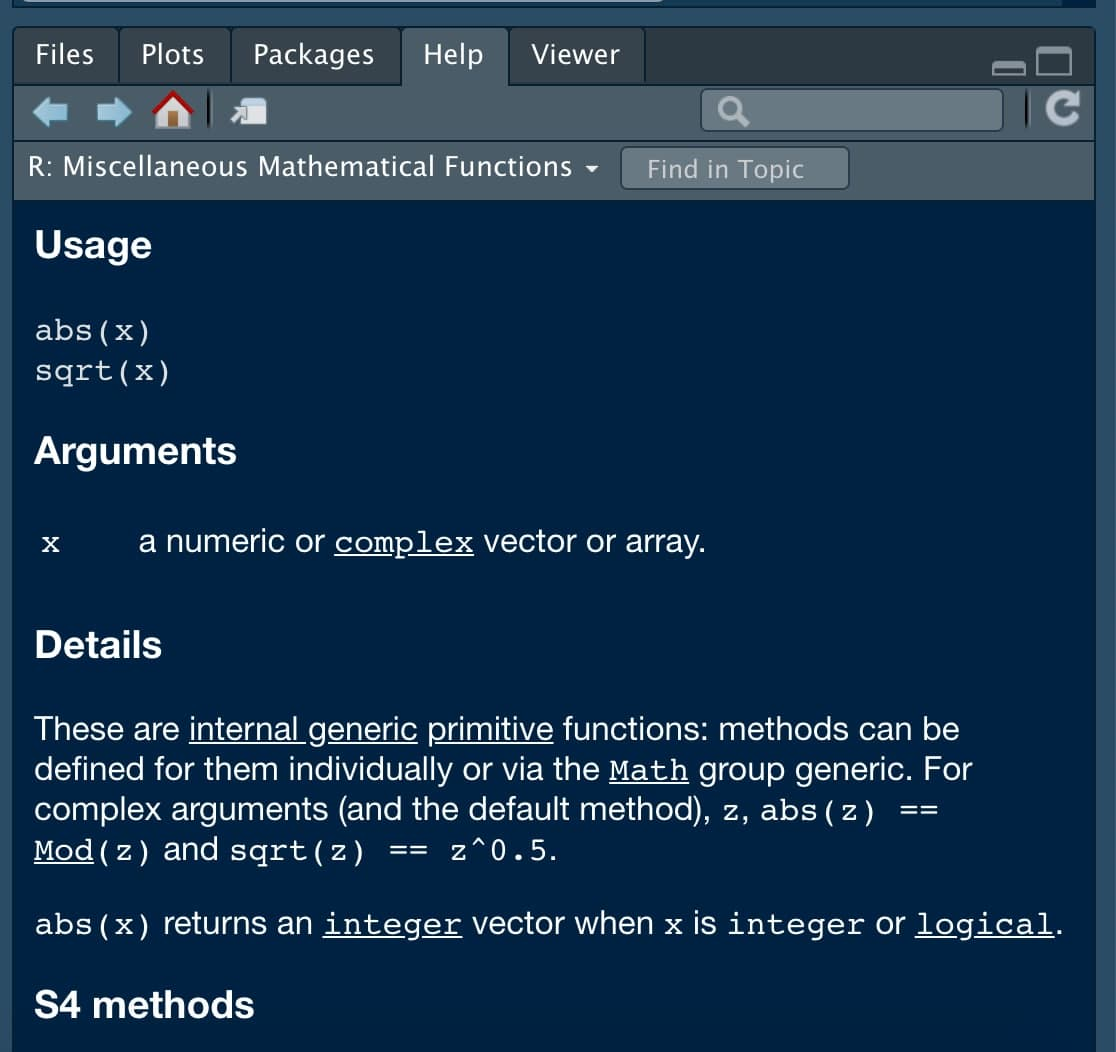
\includegraphics[width=0.5\linewidth]{./img/panel_ayuda} 

}

\caption{Panel de ayuda.}\label{fig:unnamed-chunk-9}
\end{figure}

\hypertarget{ejercicios}{%
\section{📝 Ejercicios}\label{ejercicios}}

📝Ejercicio 1: calcula en consola la suma de 3 más 4, y todo ello multiplicado por 10, y asígnalo a una variable \texttt{x}.

\begin{itemize}
\tightlist
\item
  Solución:
\end{itemize}

\begin{Shaded}
\begin{Highlighting}[]
\NormalTok{x <-}\StringTok{ }\NormalTok{(}\DecValTok{3} \OperatorTok{+}\StringTok{ }\DecValTok{4}\NormalTok{) }\OperatorTok{*}\StringTok{ }\DecValTok{10}
\end{Highlighting}
\end{Shaded}

~

📝Ejercicio 2: usando la variable \texttt{x} ya definida, calcula \texttt{x\ -\ 5} y guárdalo en una nueva variable \texttt{y}.

\begin{itemize}
\tightlist
\item
  Solución:
\end{itemize}

\begin{Shaded}
\begin{Highlighting}[]
\NormalTok{y <-}\StringTok{ }\NormalTok{x }\OperatorTok{-}\StringTok{ }\DecValTok{5}
\NormalTok{y}
\end{Highlighting}
\end{Shaded}

\begin{verbatim}
## [1] 65
\end{verbatim}

~

📝Ejercicio 3: usando las variables \texttt{x} e \texttt{y} ya definidas, calcula la raíz cuadrada del máximo entre ambas, y guárdalo en una nueva variable \texttt{z}.

\begin{itemize}
\tightlist
\item
  Solución:
\end{itemize}

\begin{Shaded}
\begin{Highlighting}[]
\NormalTok{z <-}\StringTok{ }\KeywordTok{sqrt}\NormalTok{(}\KeywordTok{max}\NormalTok{(x, y)) }\CommentTok{# No hace falta gastar una línea por cada orden (cada asignación que hagas es una variable guardada que consume memoria en tu ordenador)}
\NormalTok{z}
\end{Highlighting}
\end{Shaded}

\begin{verbatim}
## [1] 8.3666
\end{verbatim}

\hypertarget{part-conceptos-buxe1sicos}{%
\part{Conceptos básicos}\label{part-conceptos-buxe1sicos}}

\hypertarget{tipos-de-datos-i-vectores}{%
\chapter{Tipos de datos I: vectores}\label{tipos-de-datos-i-vectores}}

Bien, ya controlamos la calculadora. Vamos a ir más allá: ¿y si en lugar de tener un solo número tenemos un \textbf{CONJUNTO de elementos}? En este capítulo vamos a ver un clásico de cualquier lenguaje de programación: los \textbf{vectores o arrays}.

\hypertarget{vectores-numuxe9ricos}{%
\section{Vectores numéricos}\label{vectores-numuxe9ricos}}

Un conjunto de elementos del mismo tipo se llama \textbf{vector} (en este caso de números), y de hecho un número individual (por ejemplo, \texttt{1}) es en realidad un vector de longitud uno (un solo elemento).

La forma más sencilla de \textbf{crear un vector} en \texttt{R} es con el comando \texttt{c()} (de \textbf{concatenar elementos}), y basta con introducir sus elementos entre paréntesis, y separados por comas. Vamos a crear el vector con los tres primeros números naturales pares (el 0 no es natural, no seas bárbaro/a).

\begin{Shaded}
\begin{Highlighting}[]
\NormalTok{z <-}\StringTok{ }\KeywordTok{c}\NormalTok{(}\DecValTok{2}\NormalTok{, }\DecValTok{4}\NormalTok{, }\DecValTok{6}\NormalTok{)}
\NormalTok{z}
\end{Highlighting}
\end{Shaded}

\begin{verbatim}
## [1] 2 4 6
\end{verbatim}

Como ves ahora en el \textbf{environment tenemos una colección de elementos}, tres en concreto, guardados en una misma variable. La longitud de un vector se puede calcular con el comando \texttt{length()}.

\begin{Shaded}
\begin{Highlighting}[]
\KeywordTok{length}\NormalTok{(z)}
\end{Highlighting}
\end{Shaded}

\begin{verbatim}
## [1] 3
\end{verbatim}

Además podemos \textbf{concatenar a su vez vectores}: vamos a concatenar el vector \texttt{z} consigo mismo, y añadiéndole al final un 8.

\begin{Shaded}
\begin{Highlighting}[]
\KeywordTok{c}\NormalTok{(z, z, }\DecValTok{8}\NormalTok{)}
\end{Highlighting}
\end{Shaded}

\begin{verbatim}
## [1] 2 4 6 2 4 6 8
\end{verbatim}

La última concatenación lo que nos ha dado son los tres primeros pares, después de nuevo los tres primeros pares, y por último un 8.

\hypertarget{secuencias-con-un-patruxf3n}{%
\subsection{Secuencias con un patrón}\label{secuencias-con-un-patruxf3n}}

Muchas veces nos gustaría \textbf{crear vectores de una forma mucho más rápida}, por ejemplo, para tener un vector de índices que queramos recorrer. Supongamos que queremos el vector de los primeros 21 números naturales. Si construyéramos el vector como antes, tendríamos ejecutar el comando \texttt{c(1,\ 2,\ 3,\ 4,\ 5,\ ...)} hasta el número 21. ¿Un poco largo, no?

El comando \texttt{seq()} nos permite crear una \textbf{secuencia desde un elemento inicial hasta un elemento final, avanzando de uno en uno}.

\begin{Shaded}
\begin{Highlighting}[]
\KeywordTok{seq}\NormalTok{(}\DecValTok{1}\NormalTok{, }\DecValTok{21}\NormalTok{) }\CommentTok{# secuencia desde 1 hasta 21 de uno en uno}
\end{Highlighting}
\end{Shaded}

\begin{verbatim}
##  [1]  1  2  3  4  5  6  7  8  9 10 11 12 13 14 15 16 17 18 19 20 21
\end{verbatim}

Es importante que no perdamos el foco de que \textbf{programar es similar a escribir en un idioma}, por lo que si hay algo que se puede decir de una forma más limpia y que se entienda mejor, ¿por qué no usarlo? Siempre que queramos definir secuencias entre dos números naturales (por ejemplo, entre \texttt{1} y un valor \texttt{n}), cuya distancia entre elementos consecutivos sea uno, el comando \texttt{1:n} nos devuelve lo mismo que la orden \texttt{seq(1,\ n)}. Además, si el elemento inicial es mayor que el final, \texttt{R} entenderá solo que la secuencia la queremo decreciente.

\begin{Shaded}
\begin{Highlighting}[]
\NormalTok{n <-}\StringTok{ }\DecValTok{21}
\DecValTok{1}\OperatorTok{:}\NormalTok{n }\CommentTok{# secuencia desde 1 hasta n (21) de uno en uno}
\end{Highlighting}
\end{Shaded}

\begin{verbatim}
##  [1]  1  2  3  4  5  6  7  8  9 10 11 12 13 14 15 16 17 18 19 20 21
\end{verbatim}

\begin{Shaded}
\begin{Highlighting}[]
\DecValTok{17}\OperatorTok{:}\DecValTok{1} \CommentTok{# secuencia decreciente de 17 a 1}
\end{Highlighting}
\end{Shaded}

\begin{verbatim}
##  [1] 17 16 15 14 13 12 11 10  9  8  7  6  5  4  3  2  1
\end{verbatim}

~

También podemos definir \textbf{otro tipo de distancia entre dos elementos consecutivos} (conocido como \textbf{paso de discretización}), por ejemplo de 0.5 en 0.5, o bien definir una secuencia entre un valor inicial y un valor final con un número de elementos fijo (y que sea \texttt{R} el que decida la distancia entre elementos consecutivos).

\begin{Shaded}
\begin{Highlighting}[]
\KeywordTok{seq}\NormalTok{(}\DecValTok{1}\NormalTok{, }\DecValTok{10}\NormalTok{, }\DataTypeTok{by =} \FloatTok{0.5}\NormalTok{) }\CommentTok{# secuencia desde 1 a 10 de 0.5 en 0.5}
\end{Highlighting}
\end{Shaded}

\begin{verbatim}
##  [1]  1.0  1.5  2.0  2.5  3.0  3.5  4.0  4.5  5.0  5.5  6.0  6.5  7.0  7.5  8.0
## [16]  8.5  9.0  9.5 10.0
\end{verbatim}

\begin{Shaded}
\begin{Highlighting}[]
\KeywordTok{seq}\NormalTok{(}\DecValTok{1}\NormalTok{, }\DecValTok{50}\NormalTok{, }\DataTypeTok{l =} \DecValTok{11}\NormalTok{) }\CommentTok{# secuencia desde 1 a 100 de longitud 11}
\end{Highlighting}
\end{Shaded}

\begin{verbatim}
##  [1]  1.0  5.9 10.8 15.7 20.6 25.5 30.4 35.3 40.2 45.1 50.0
\end{verbatim}

~

Otro atajo que podemos usar para definir secuencias de números con un patrón es definir \textbf{vectores repetidos}, por ejemplo un vector lleno de 0, para luego ser rellenado (pero ya tenerlo definido). La función \texttt{rep()} nos permite repetir un elemento un número fijado de veces.

\begin{Shaded}
\begin{Highlighting}[]
\KeywordTok{rep}\NormalTok{(}\DecValTok{0}\NormalTok{, }\DecValTok{7}\NormalTok{) }\CommentTok{# vector de 7 ceros}
\end{Highlighting}
\end{Shaded}

\begin{verbatim}
## [1] 0 0 0 0 0 0 0
\end{verbatim}

No solo podemos repetir un número sino que podemos repetir vectores enteros.

\begin{Shaded}
\begin{Highlighting}[]
\KeywordTok{rep}\NormalTok{(}\KeywordTok{c}\NormalTok{(}\DecValTok{0}\NormalTok{, }\DecValTok{1}\NormalTok{, }\DecValTok{2}\NormalTok{), }\DecValTok{4}\NormalTok{) }\CommentTok{# repetimos el vector c(0, 1, 2) 4 veces}
\end{Highlighting}
\end{Shaded}

\begin{verbatim}
##  [1] 0 1 2 0 1 2 0 1 2 0 1 2
\end{verbatim}

Esa repetición además podemos definirla también de forma \textbf{intercalada}: en lugar de repetir \texttt{c(0,\ 1,\ 2)} cuatro veces seguidas, queremos cuatro 0, después cuatro 1, y después cuatro 2.

\begin{Shaded}
\begin{Highlighting}[]
\KeywordTok{rep}\NormalTok{(}\KeywordTok{c}\NormalTok{(}\DecValTok{0}\NormalTok{, }\DecValTok{1}\NormalTok{, }\DecValTok{2}\NormalTok{), }\DataTypeTok{each =} \DecValTok{4}\NormalTok{) }\CommentTok{# cuatro 0, luego cuatro 1, luego cuatro 2}
\end{Highlighting}
\end{Shaded}

\begin{verbatim}
##  [1] 0 0 0 0 1 1 1 1 2 2 2 2
\end{verbatim}

\hypertarget{operaciones-aritmuxe9ticas-con-vectores-numuxe9ricos}{%
\section{Operaciones aritméticas con vectores numéricos}\label{operaciones-aritmuxe9ticas-con-vectores-numuxe9ricos}}

Hemos dicho que un número es un vector de longitud 1, así que \textbf{toda operación aritmética} que podamos hacer con un número la vamos a poder a hacer con un vector de números, de forma que si hacemos por ejemplo la operación \texttt{2\ *\ z}, lo que sucederá es \textbf{CADA ELEMENTO del vector} será multiplicado 2. De la misma manera se pueden definir sumas \texttt{z\ +\ x}, raíces cuadradas \texttt{sqrt(z)} o elevar cada elemento al cuadrado \texttt{z\^{}2}.

\begin{Shaded}
\begin{Highlighting}[]
\NormalTok{z <-}\StringTok{ }\KeywordTok{c}\NormalTok{(}\DecValTok{2}\NormalTok{, }\DecValTok{4}\NormalTok{, }\DecValTok{6}\NormalTok{)}
\DecValTok{2} \OperatorTok{*}\StringTok{ }\NormalTok{z}
\end{Highlighting}
\end{Shaded}

\begin{verbatim}
## [1]  4  8 12
\end{verbatim}

\begin{Shaded}
\begin{Highlighting}[]
\NormalTok{x <-}\StringTok{ }\DecValTok{1} \OperatorTok{+}\StringTok{ }\DecValTok{2}
\NormalTok{z }\OperatorTok{+}\StringTok{ }\NormalTok{x}
\end{Highlighting}
\end{Shaded}

\begin{verbatim}
## [1] 5 7 9
\end{verbatim}

\begin{Shaded}
\begin{Highlighting}[]
\KeywordTok{sqrt}\NormalTok{(z)}
\end{Highlighting}
\end{Shaded}

\begin{verbatim}
## [1] 1.414214 2.000000 2.449490
\end{verbatim}

\begin{Shaded}
\begin{Highlighting}[]
\NormalTok{z}\OperatorTok{^}\DecValTok{2}
\end{Highlighting}
\end{Shaded}

\begin{verbatim}
## [1]  4 16 36
\end{verbatim}

Dado que la operación (por ejemplo, una suma) se realiza elemento a elemento, \textbf{¿qué sucederá si sumamos dos vectores de distinta longitud?} Prueba a definir un vector con los 4 primeros imparos y súmale a z.

\begin{Shaded}
\begin{Highlighting}[]
\NormalTok{y <-}\StringTok{ }\KeywordTok{c}\NormalTok{(}\DecValTok{1}\NormalTok{, }\DecValTok{3}\NormalTok{, }\DecValTok{5}\NormalTok{, }\DecValTok{7}\NormalTok{)}
\NormalTok{variable_suma <-}\StringTok{ }\NormalTok{z }\OperatorTok{+}\StringTok{ }\NormalTok{y}
\end{Highlighting}
\end{Shaded}

\begin{verbatim}
## Warning in z + y: longitud de objeto mayor no es múltiplo de la longitud de uno
## menor
\end{verbatim}

\begin{Shaded}
\begin{Highlighting}[]
\NormalTok{variable_suma}
\end{Highlighting}
\end{Shaded}

\begin{verbatim}
## [1]  3  7 11  9
\end{verbatim}

Como ves, \texttt{R} intenta molestarte lo menos posible, así que lo hace es reciclar: si tiene un vector de 4 elementos y le intentas sumar uno de 3 elementos, lo que hará será \textbf{reciclar} elementos del vector con menor longitud: hará \texttt{1+2}, \texttt{3+4}, \texttt{5+6} pero\ldots{} \texttt{7+2} (vuelve al primer par).

\hypertarget{operaciones-estaduxedsticas-con-vectores-numuxe9ricos}{%
\section{Operaciones estadísticas con vectores numéricos}\label{operaciones-estaduxedsticas-con-vectores-numuxe9ricos}}

Al igual que podemos ejecutar operaciones aritméticas, podemos realizar también \textbf{operaciones estadísticas} con los vectores, como calcular su suma (\texttt{sum()}), su media (\texttt{mean()}), su mediana (\texttt{median()}), su suma acumulada (\texttt{cumsum()} cada elemento lo acumula al anterior) o percentiles (\texttt{quantiles()}).

\begin{Shaded}
\begin{Highlighting}[]
\KeywordTok{sum}\NormalTok{(y) }\CommentTok{# suma}
\end{Highlighting}
\end{Shaded}

\begin{verbatim}
## [1] 16
\end{verbatim}

\begin{Shaded}
\begin{Highlighting}[]
\KeywordTok{mean}\NormalTok{(y) }\CommentTok{# media}
\end{Highlighting}
\end{Shaded}

\begin{verbatim}
## [1] 4
\end{verbatim}

\begin{Shaded}
\begin{Highlighting}[]
\KeywordTok{median}\NormalTok{(y) }\CommentTok{# mediana}
\end{Highlighting}
\end{Shaded}

\begin{verbatim}
## [1] 4
\end{verbatim}

\begin{Shaded}
\begin{Highlighting}[]
\KeywordTok{cumsum}\NormalTok{(y) }\CommentTok{# suma acumulada}
\end{Highlighting}
\end{Shaded}

\begin{verbatim}
## [1]  1  4  9 16
\end{verbatim}

\begin{Shaded}
\begin{Highlighting}[]
\NormalTok{y <-}\StringTok{ }\KeywordTok{c}\NormalTok{(}\DecValTok{1}\NormalTok{, }\DecValTok{2}\NormalTok{, }\DecValTok{5}\NormalTok{, }\DecValTok{5}\NormalTok{, }\DecValTok{8}\NormalTok{, }\DecValTok{9}\NormalTok{, }\DecValTok{10}\NormalTok{, }\DecValTok{10}\NormalTok{, }\DecValTok{10}\NormalTok{, }\DecValTok{11}\NormalTok{, }\DecValTok{13}\NormalTok{, }\DecValTok{15}\NormalTok{, }\DecValTok{20}\NormalTok{, }\DecValTok{23}\NormalTok{, }\DecValTok{24}\NormalTok{, }\DecValTok{29}\NormalTok{)}
\KeywordTok{quantile}\NormalTok{(y, }\DataTypeTok{probs =} \KeywordTok{c}\NormalTok{(}\FloatTok{0.15}\NormalTok{, }\FloatTok{0.3}\NormalTok{, }\FloatTok{0.7}\NormalTok{, }\FloatTok{0.9}\NormalTok{)) }\CommentTok{# Percentiles p15, p30, p70 y p90}
\end{Highlighting}
\end{Shaded}

\begin{verbatim}
##  15%  30%  70%  90% 
##  5.0  8.5 14.0 23.5
\end{verbatim}

Ver conceptos básicos en \ref{glosario3}.

\hypertarget{vectores-de-caracteres-texto}{%
\section{Vectores de caracteres (texto)}\label{vectores-de-caracteres-texto}}

Un error común es asociar vectores solo a números: un \textbf{vector es una colección de elementos del mismo tipo} pero no tienen porque ser necesariamente números. Vamos a crear una frase de ejemplo, un vector de 4 elementos de tipo texto (en \texttt{R} se llaman \texttt{char}): \texttt{"Mi"}, \texttt{"nombre"}, \texttt{"es"} \texttt{"Javier"}.

Como ves las variables de tipo \texttt{char} van entre comillas dobles, ya que es un \textbf{cadena de texto}.

\begin{Shaded}
\begin{Highlighting}[]
\NormalTok{mi_nombre <-}\StringTok{ }\KeywordTok{c}\NormalTok{(}\StringTok{"Mi"}\NormalTok{, }\StringTok{"nombre"}\NormalTok{, }\StringTok{"es"}\NormalTok{, }\StringTok{"Javier"}\NormalTok{)}
\NormalTok{mi_nombre}
\end{Highlighting}
\end{Shaded}

\begin{verbatim}
## [1] "Mi"     "nombre" "es"     "Javier"
\end{verbatim}

Ya tenemos nuestro primer vector de texto de longitud 4. Las \textbf{cadenas de texto} son un tipo especial de dato, con los que obviamente no podremos hacer operaciones aritméticas como la suma o la media, pero si podemos hacer operaciones propias de cadenas de texto como puede ser la función \texttt{paste()}. Dicha función nos permite convertir un vector de 4 palabras en una frase, decidiendo que caracter queremos que vaya entre palabra con el argumento \texttt{collapse\ =}.

\begin{Shaded}
\begin{Highlighting}[]
\KeywordTok{paste}\NormalTok{(mi_nombre, }\DataTypeTok{collapse =} \StringTok{""}\NormalTok{) }\CommentTok{# todo junto}
\end{Highlighting}
\end{Shaded}

\begin{verbatim}
## [1] "MinombreesJavier"
\end{verbatim}

\begin{Shaded}
\begin{Highlighting}[]
\KeywordTok{paste}\NormalTok{(mi_nombre, }\DataTypeTok{collapse =} \StringTok{" "}\NormalTok{) }\CommentTok{# separados por un espacio}
\end{Highlighting}
\end{Shaded}

\begin{verbatim}
## [1] "Mi nombre es Javier"
\end{verbatim}

\begin{Shaded}
\begin{Highlighting}[]
\KeywordTok{paste}\NormalTok{(mi_nombre, }\DataTypeTok{collapse =} \StringTok{"."}\NormalTok{) }\CommentTok{# separados por un punto .}
\end{Highlighting}
\end{Shaded}

\begin{verbatim}
## [1] "Mi.nombre.es.Javier"
\end{verbatim}

Si queremos pegar los elementos de la cadena de texto sin ningún tipo de caracter, existe una forma más abreviada y limpia de ejecutar la orden \texttt{paste(mi\_nombre,\ collapse\ =\ "")}, usando la función \texttt{paste0()}

\begin{Shaded}
\begin{Highlighting}[]
\KeywordTok{paste0}\NormalTok{(mi_nombre) }\CommentTok{# todo junto sin nada separando}
\end{Highlighting}
\end{Shaded}

\begin{verbatim}
## [1] "Mi"     "nombre" "es"     "Javier"
\end{verbatim}

Esta función es muy útil si queremos definir variables de texto que compartan por ejemplo un prefijo (\texttt{variable\_1}, \texttt{variable\_2}, \ldots{})

\begin{Shaded}
\begin{Highlighting}[]
\KeywordTok{paste0}\NormalTok{(}\StringTok{"variable"}\NormalTok{, }\DecValTok{1}\OperatorTok{:}\DecValTok{7}\NormalTok{) }\CommentTok{# a la palabra «variable» le pegamos los números del 1 al 7}
\end{Highlighting}
\end{Shaded}

\begin{verbatim}
## [1] "variable1" "variable2" "variable3" "variable4" "variable5" "variable6"
## [7] "variable7"
\end{verbatim}

\begin{Shaded}
\begin{Highlighting}[]
\KeywordTok{paste}\NormalTok{(}\StringTok{"variable"}\NormalTok{, }\DecValTok{1}\OperatorTok{:}\DecValTok{7}\NormalTok{, }\DataTypeTok{sep =} \StringTok{"_"}\NormalTok{) }\CommentTok{# separado por una barra baja}
\end{Highlighting}
\end{Shaded}

\begin{verbatim}
## [1] "variable_1" "variable_2" "variable_3" "variable_4" "variable_5"
## [6] "variable_6" "variable_7"
\end{verbatim}

~

Otra \textbf{forma más intuitiva de trabajar con textos y variables numéricas} es usar el paquete \texttt{\{glue\}}, que nos permite pegar cadenas de texto a variables numéricas de \textbf{forma simbólica}.

\begin{Shaded}
\begin{Highlighting}[]
\KeywordTok{install.packages}\NormalTok{(}\StringTok{"glue"}\NormalTok{)}
\KeywordTok{library}\NormalTok{(glue)}
\NormalTok{edad <-}\StringTok{ }\DecValTok{10}\OperatorTok{:}\DecValTok{15} \CommentTok{# edades}
\KeywordTok{glue}\NormalTok{(}\StringTok{"La edad es de \{edad\} años"}\NormalTok{)}
\end{Highlighting}
\end{Shaded}

\begin{verbatim}
## La edad es de 10 años
## La edad es de 11 años
## La edad es de 12 años
## La edad es de 13 años
## La edad es de 14 años
## La edad es de 15 años
\end{verbatim}

\begin{Shaded}
\begin{Highlighting}[]
\CommentTok{# Otra forma sin definir variables a priori}
\KeywordTok{glue}\NormalTok{(}\StringTok{"La edad es de \{10:15\} años"}\NormalTok{)}
\end{Highlighting}
\end{Shaded}

\begin{verbatim}
## La edad es de 10 años
## La edad es de 11 años
## La edad es de 12 años
## La edad es de 13 años
## La edad es de 14 años
## La edad es de 15 años
\end{verbatim}

~

Ya sabemos trabajar con textos :)

¿Y si queremos \textbf{pasar todo a mayúscula}? ¿O \textbf{todo a minúscula}? ¿Y si queremos \textbf{sustituir un caracter (por ejemplo \texttt{.}) por otro en todos los elementos}? \texttt{R} también nos proporciona algunas funciones muy sencillas de usar para dichas tareas. Aquí un ejemplo de algunas de ellas.

\begin{Shaded}
\begin{Highlighting}[]
\NormalTok{texto <-}\StringTok{ }\KeywordTok{c}\NormalTok{(}\StringTok{"Hola."}\NormalTok{, }\StringTok{"qué"}\NormalTok{, }\StringTok{"ase?"}\NormalTok{, }\StringTok{"todo"}\NormalTok{, }\StringTok{"bien."}\NormalTok{, }\StringTok{"y yo"}\NormalTok{,}
           \StringTok{"que"}\NormalTok{, }\StringTok{"ME"}\NormalTok{, }\StringTok{"ALEGRO"}\NormalTok{)}
\KeywordTok{toupper}\NormalTok{(texto) }\CommentTok{# todo a mayúscula}
\end{Highlighting}
\end{Shaded}

\begin{verbatim}
## [1] "HOLA."  "QUÉ"    "ASE?"   "TODO"   "BIEN."  "Y YO"   "QUE"    "ME"    
## [9] "ALEGRO"
\end{verbatim}

\begin{Shaded}
\begin{Highlighting}[]
\KeywordTok{tolower}\NormalTok{(texto) }\CommentTok{# todo a minúscula}
\end{Highlighting}
\end{Shaded}

\begin{verbatim}
## [1] "hola."  "qué"    "ase?"   "todo"   "bien."  "y yo"   "que"    "me"    
## [9] "alegro"
\end{verbatim}

\begin{Shaded}
\begin{Highlighting}[]
\KeywordTok{gsub}\NormalTok{(}\StringTok{"o"}\NormalTok{, }\StringTok{"*"}\NormalTok{, texto) }\CommentTok{# toda "o" en el texto será sustituida por *}
\end{Highlighting}
\end{Shaded}

\begin{verbatim}
## [1] "H*la."  "qué"    "ase?"   "t*d*"   "bien."  "y y*"   "que"    "ME"    
## [9] "ALEGRO"
\end{verbatim}

~

\begin{figure}
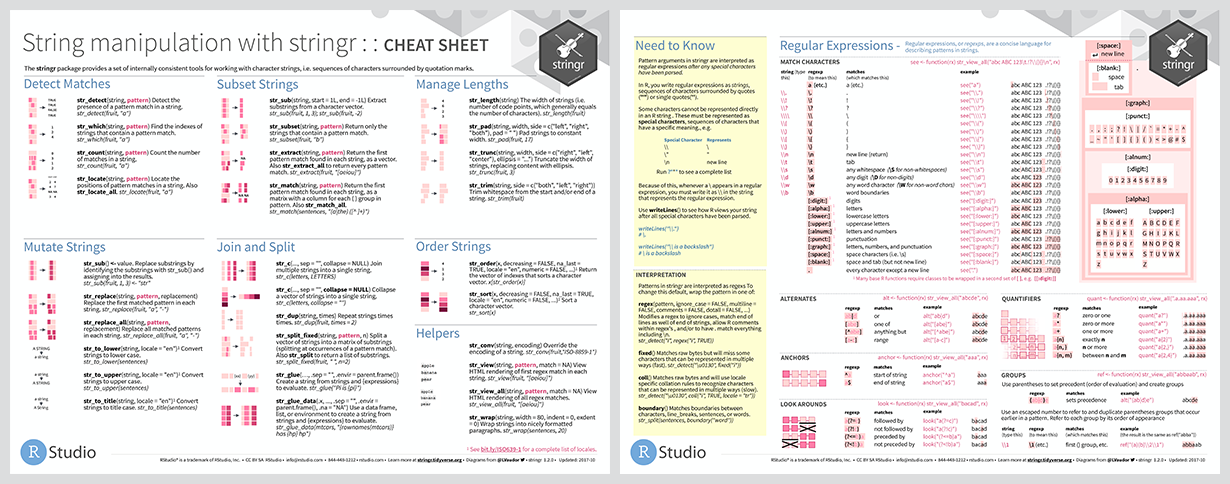
\includegraphics[width=17.08in]{./img/stringr} \caption{Paquete stringr para manejar cadenas de texto más complejas}\label{fig:stringr2}
\end{figure}

\hypertarget{vectores-luxf3gicos-truefalse}{%
\section{Vectores lógicos (TRUE/FALSE)}\label{vectores-luxf3gicos-truefalse}}

\begin{itemize}
\tightlist
\item
  {[}X{]} Variables numéricas (individuales)
\item
  {[}X{]} Vectores de números
\item
  {[}X{]} Vectores de caracteres
\item
  {[} {]} Vectores lógicos
\end{itemize}

Veamos un último tipo de vectores importante en todo lenguaje de programación: los \textbf{vectores lógicos}. Un \textbf{valor lógico} puede tomar tres valores: \texttt{TRUE} (guardado internamente como un \texttt{1}), \texttt{FALSE} (guardado internamente como un \texttt{0}) o \texttt{NA} (dato ausente, son las siglas de \emph{not available}). Estos valores son resultado de evaluar \textbf{condiciones lógicas}.

Por ejemplo, imaginemos que definimos un vector de números \texttt{x\ \textless{}-\ c(1.5,\ -1,\ 2,\ 4,\ 3,\ -4)}. ¿Qué numeros del vector son menores que 2? Basta con que ejecutemos la orden \texttt{x\ \textless{}\ 2}, que nos devolverá \texttt{TRUE/FALSE} en cada hueco, en función de si cumple (\texttt{TRUE}) o no (\texttt{FALSE}) la condición pedida.

\begin{Shaded}
\begin{Highlighting}[]
\NormalTok{x <-}\StringTok{ }\KeywordTok{c}\NormalTok{(}\FloatTok{1.5}\NormalTok{, }\DecValTok{-1}\NormalTok{, }\DecValTok{2}\NormalTok{, }\DecValTok{4}\NormalTok{, }\DecValTok{3}\NormalTok{, }\DecValTok{-4}\NormalTok{)}
\NormalTok{x }\OperatorTok{<}\StringTok{ }\DecValTok{2}
\end{Highlighting}
\end{Shaded}

\begin{verbatim}
## [1]  TRUE  TRUE FALSE FALSE FALSE  TRUE
\end{verbatim}

El primer, segundo y sexto elemento del vector son los únicos elementos (estrictamente) menores que \texttt{2}, de ahí que en el primer, segundo y sexto elemento aparezca un \texttt{TRUE} y en el resto un \texttt{FALSE}. Es \textbf{importante} recordar que al \textbf{evaluar una condición lógica sobre un vector} de longitud \texttt{n}, la \textbf{salida sigue siendo un vector} de longitud \texttt{n} pero con valores lógicos.

Dicha condición lógica puede hacerse con otros operadores como \texttt{\textless{}=}, \texttt{\textgreater{}} o \texttt{\textgreater{}=}.

\begin{Shaded}
\begin{Highlighting}[]
\NormalTok{x }\OperatorTok{<=}\StringTok{ }\DecValTok{2}
\end{Highlighting}
\end{Shaded}

\begin{verbatim}
## [1]  TRUE  TRUE  TRUE FALSE FALSE  TRUE
\end{verbatim}

\begin{Shaded}
\begin{Highlighting}[]
\NormalTok{x }\OperatorTok{>}\StringTok{ }\DecValTok{2}
\end{Highlighting}
\end{Shaded}

\begin{verbatim}
## [1] FALSE FALSE FALSE  TRUE  TRUE FALSE
\end{verbatim}

\begin{Shaded}
\begin{Highlighting}[]
\NormalTok{x }\OperatorTok{>=}\StringTok{ }\DecValTok{2}
\end{Highlighting}
\end{Shaded}

\begin{verbatim}
## [1] FALSE FALSE  TRUE  TRUE  TRUE FALSE
\end{verbatim}

~

También podemos \textbf{comparar si es igual a otro elemento}, para lo que usaremos el operador \texttt{==}, pudiendo usar también su opuesto \texttt{!=} (distinto de).

\begin{Shaded}
\begin{Highlighting}[]
\NormalTok{x }\OperatorTok{==}\StringTok{ }\DecValTok{2}
\end{Highlighting}
\end{Shaded}

\begin{verbatim}
## [1] FALSE FALSE  TRUE FALSE FALSE FALSE
\end{verbatim}

\begin{Shaded}
\begin{Highlighting}[]
\NormalTok{x }\OperatorTok{!=}\StringTok{ }\DecValTok{2}
\end{Highlighting}
\end{Shaded}

\begin{verbatim}
## [1]  TRUE  TRUE FALSE  TRUE  TRUE  TRUE
\end{verbatim}

Las \textbf{condiciones pueden ser combinadas}, principalmente de dos maneras:

\begin{itemize}
\item
  \textbf{Intersección}: todas las condiciones concatenadas se deben cumplir (conjunción \texttt{y}, operador \texttt{\&}) para devolver un \texttt{TRUE}.
\item
  \textbf{Unión}: basta con que una de las condiciones concatenadas se cumpla (conjunción \texttt{o}, operador \texttt{\textbar{}}) para devolver un \texttt{TRUE}.
\end{itemize}

Por ejemplo, vamos a calcular qué elementos del vector \texttt{c(1.5,\ -1,\ 2,\ 4,\ 3,\ -4)} sean menores que 3 pero (y) mayores que 0, y los elementos menores que 2 o mayores que 3.

\begin{Shaded}
\begin{Highlighting}[]
\NormalTok{x <-}\StringTok{ }\KeywordTok{c}\NormalTok{(}\FloatTok{1.5}\NormalTok{, }\DecValTok{-1}\NormalTok{, }\DecValTok{2}\NormalTok{, }\DecValTok{4}\NormalTok{, }\DecValTok{3}\NormalTok{, }\DecValTok{-4}\NormalTok{)}
\NormalTok{x }\OperatorTok{<}\StringTok{ }\DecValTok{3} \OperatorTok{&}\StringTok{ }\NormalTok{x }\OperatorTok{>}\StringTok{ }\DecValTok{0} \CommentTok{# Solo los que cumplen ambas condiciones}
\end{Highlighting}
\end{Shaded}

\begin{verbatim}
## [1]  TRUE FALSE  TRUE FALSE FALSE FALSE
\end{verbatim}

\begin{Shaded}
\begin{Highlighting}[]
\NormalTok{x }\OperatorTok{<}\StringTok{ }\DecValTok{2} \OperatorTok{|}\StringTok{ }\NormalTok{x }\OperatorTok{>}\StringTok{ }\DecValTok{3} \CommentTok{# Los cumplen al menos una de ellas}
\end{Highlighting}
\end{Shaded}

\begin{verbatim}
## [1]  TRUE  TRUE FALSE  TRUE FALSE  TRUE
\end{verbatim}

Como hemos comentado anteriormente, los valores lógicos \texttt{TRUE/FALSE} son guardados internamente como \texttt{0/1} por lo que podemos usar \textbf{operaciones aritméticas con ellos}. Por ejemplo, si queremos averiguar el número de elementos de un vector que cumplen una condición lógica \texttt{\textless{}\ 2}, los que lo hagan tendrán asignado un \texttt{1} y los que no un \texttt{0}, por lo que basta con sumar el vector lógico para obtener el número de elementos bajo dicha condición.

\begin{Shaded}
\begin{Highlighting}[]
\KeywordTok{sum}\NormalTok{(x }\OperatorTok{<}\StringTok{ }\DecValTok{2}\NormalTok{) }\CommentTok{# sumamos el vector de TRUE/FALSE --> número de TRUE}
\end{Highlighting}
\end{Shaded}

\begin{verbatim}
## [1] 3
\end{verbatim}

\hypertarget{ausentes}{%
\section{Datos ausentes: NA y NaN}\label{ausentes}}

La vida no siempre es perfecta así en muchas ocasiones nos encontraremos con lo que llamamos en estadística un \textbf{dato ausente o \emph{missing value}}, un \textbf{valor que no tenemos en nuestra variable}, y un ejemplo práctico lo tenemos con los datos de vacunación de covid del Ministerio de Sanidad. Cada día se publicaba un PDF (ya\ldots{}mal) con los datos de vacunación PERO\ldots{}no se publican datos los fines de semana: en dichas fechas hay datos que no tenemos, y en \texttt{R} se representan por \texttt{NA} (significa \emph{not available}). Vamos a crear un vector de números con datos ausentes con la orden \texttt{x\ \textless{}-\ c(1,\ NA,\ 3,\ NA,\ NA,\ 5,\ 6)}: el vector tendrá longitud 7 pero en el segundo, cuarto y quinto elemento tendremos un dato faltante, un lugar que no tenemos relleno (pero que no eliminamos).

\begin{Shaded}
\begin{Highlighting}[]
\NormalTok{x <-}\StringTok{ }\KeywordTok{c}\NormalTok{(}\DecValTok{1}\NormalTok{, }\OtherTok{NA}\NormalTok{, }\DecValTok{3}\NormalTok{, }\OtherTok{NA}\NormalTok{, }\OtherTok{NA}\NormalTok{, }\DecValTok{5}\NormalTok{, }\DecValTok{6}\NormalTok{) }\CommentTok{# Vector numérico con datos faltante}
\KeywordTok{length}\NormalTok{(x) }\CommentTok{# longitud del vector}
\end{Highlighting}
\end{Shaded}

\begin{verbatim}
## [1] 7
\end{verbatim}

\begin{Shaded}
\begin{Highlighting}[]
\NormalTok{x}
\end{Highlighting}
\end{Shaded}

\begin{verbatim}
## [1]  1 NA  3 NA NA  5  6
\end{verbatim}

\textbf{¿Puedes aventurar que sucede cuando multiplicamos ese vector por 2 por ejemplo?}

\begin{Shaded}
\begin{Highlighting}[]
\DecValTok{2} \OperatorTok{*}\StringTok{ }\NormalTok{x }\CommentTok{# operación aritmética con un vector con NA}
\end{Highlighting}
\end{Shaded}

\begin{verbatim}
## [1]  2 NA  6 NA NA 10 12
\end{verbatim}

Efectivamente: un dato que no tenemos, multiplicado por 2, sigue siendo un dato ausente. Es muy importante para evitar resultados erróneos que entendamos que un \textbf{dato ausente no computa en una operación aritmética, es un hueco vacío}. Si hacemos la suma del vector, estamos sumando números más datos ausentes, por lo que el resultado final será también un dato ausente. Si tenemos algún dato ausente en nuestro vector, la suma final está a su vez ausente, ¡no podemos saber cuánto vale!

\begin{Shaded}
\begin{Highlighting}[]
\KeywordTok{sum}\NormalTok{(x) }\CommentTok{# suma de un vector que contiene NA}
\end{Highlighting}
\end{Shaded}

\begin{verbatim}
## [1] NA
\end{verbatim}

Para evitar que un dato ausente en nuestros datos nos impida hacer ciertas operaciones, en muchas funciones de \texttt{R} podemos añadir el argumento \texttt{na.rm\ =\ TRUE}: \textbf{primero elimina los datos ausentes}, y luego ejecuta la función.

\begin{Shaded}
\begin{Highlighting}[]
\KeywordTok{sum}\NormalTok{(x, }\DataTypeTok{na.rm =} \OtherTok{TRUE}\NormalTok{) }\CommentTok{# eliminando datos ausentes}
\end{Highlighting}
\end{Shaded}

\begin{verbatim}
## [1] 15
\end{verbatim}

Una manera de \textbf{localizar que elementos están ausentes} en nuestras variables es con la función \texttt{is.na()}, una función que nos devuelve un vector de valores lógico: \texttt{TRUE} si el elemento está ausente y \texttt{FALSE} si no lo está.

\begin{Shaded}
\begin{Highlighting}[]
\KeywordTok{is.na}\NormalTok{(x) }\CommentTok{# TRUE si está ausente (NA), FALSE si no lo está.}
\end{Highlighting}
\end{Shaded}

\begin{verbatim}
## [1] FALSE  TRUE FALSE  TRUE  TRUE FALSE FALSE
\end{verbatim}

Dichos \textbf{datos ausentes se pueden eliminar} (sin necesidad de sumarlos) con la función \texttt{na.omit()} (aunque a veces lo que nos interesa es que no sea ausente, introduciendo el punto medio entre su valor anterior y su valor posterior, por ejemplo).

\begin{Shaded}
\begin{Highlighting}[]
\KeywordTok{na.omit}\NormalTok{(x)}
\end{Highlighting}
\end{Shaded}

\begin{verbatim}
## [1] 1 3 5 6
## attr(,"na.action")
## [1] 2 4 5
## attr(,"class")
## [1] "omit"
\end{verbatim}

~

Hay un \textbf{tipo de dato muy particular, como resultado de operaciones no permitidas o cuyo resultado es indeterminado}, que en \texttt{R} lo veremos como \texttt{NaN}: \emph{not a number}, un resultado fruto de una indeterminación, como por ejemplo la operación \texttt{0/0} (cuyo límite no está definido). Importante saber que también existe una forma de denotar al infinito como \texttt{Inf}, siendo el resultado de algunas operaciones como \texttt{1/0} (cuyo límite si existe).

\begin{Shaded}
\begin{Highlighting}[]
\DecValTok{1}\OperatorTok{/}\DecValTok{0}
\end{Highlighting}
\end{Shaded}

\begin{verbatim}
## [1] Inf
\end{verbatim}

\begin{Shaded}
\begin{Highlighting}[]
\DecValTok{0}\OperatorTok{/}\DecValTok{0}
\end{Highlighting}
\end{Shaded}

\begin{verbatim}
## [1] NaN
\end{verbatim}

\begin{Shaded}
\begin{Highlighting}[]
\KeywordTok{sqrt}\NormalTok{(}\OperatorTok{-}\DecValTok{1}\NormalTok{)}
\end{Highlighting}
\end{Shaded}

\begin{verbatim}
## Warning in sqrt(-1): Se han producido NaNs
\end{verbatim}

\begin{verbatim}
## [1] NaN
\end{verbatim}

De la misma manera que podemos localizar valores \texttt{NA}, tenemos a nuestra disposición las funciones \texttt{is.infinte()} y \texttt{is.nan()} para detectar que elementos de nuestro vector son \texttt{Inf} o \texttt{NaN}, respectivamente.

\begin{Shaded}
\begin{Highlighting}[]
\NormalTok{x <-}\StringTok{ }\KeywordTok{c}\NormalTok{(}\DecValTok{1}\NormalTok{, }\OtherTok{NA}\NormalTok{, }\DecValTok{3}\NormalTok{, }\DecValTok{4}\NormalTok{, }\OtherTok{Inf}\NormalTok{, }\DecValTok{6}\NormalTok{, }\DecValTok{7}\NormalTok{, }\OtherTok{Inf}\NormalTok{, }\OtherTok{NaN}\NormalTok{, }\OtherTok{NA}\NormalTok{)}
\KeywordTok{is.na}\NormalTok{(x)}
\end{Highlighting}
\end{Shaded}

\begin{verbatim}
##  [1] FALSE  TRUE FALSE FALSE FALSE FALSE FALSE FALSE  TRUE  TRUE
\end{verbatim}

\begin{Shaded}
\begin{Highlighting}[]
\KeywordTok{is.nan}\NormalTok{(x)}
\end{Highlighting}
\end{Shaded}

\begin{verbatim}
##  [1] FALSE FALSE FALSE FALSE FALSE FALSE FALSE FALSE  TRUE FALSE
\end{verbatim}

\begin{Shaded}
\begin{Highlighting}[]
\KeywordTok{is.infinite}\NormalTok{(x)}
\end{Highlighting}
\end{Shaded}

\begin{verbatim}
##  [1] FALSE FALSE FALSE FALSE  TRUE FALSE FALSE  TRUE FALSE FALSE
\end{verbatim}

\hypertarget{seleccionar-elementos-de-un-vector}{%
\section{Seleccionar elementos de un vector}\label{seleccionar-elementos-de-un-vector}}

Ya sabemos definir variables que sean vectores (recuerda: colección de valores del mismo tipo).

\textbf{¿Y si del vector original queremos EXTRAER UN SUBCONJUNTO del mismo, por ejemplo, los primeros 10 elementos?}

\texttt{R} tiene varias formas de hacer esto pero la más sencilla es entendiendo que si yo quiero \textbf{acceder al elemento i} de un vector, deberé usar el \textbf{operador de selección \texttt{{[}i{]}}}. Veamos un ejemplo

\begin{Shaded}
\begin{Highlighting}[]
\NormalTok{x <-}\StringTok{ }\DecValTok{1}\OperatorTok{:}\DecValTok{100} \CommentTok{# Vector de longitud 100 (del 1 al 100)}
\NormalTok{y <-}\StringTok{ }\NormalTok{x[}\DecValTok{37}\NormalTok{] }\CommentTok{# Solo me interesa el elemento que ocupa el lugar 37}
\NormalTok{y}
\end{Highlighting}
\end{Shaded}

\begin{verbatim}
## [1] 37
\end{verbatim}

Dado que hemos visto que un número no es más que un vector de longitud uno, esta operación también la podemos aplicar usando un vector de índices a seleccionar, de forma que le podemos indicar simultaneamente que valores que queremos

\begin{Shaded}
\begin{Highlighting}[]
\NormalTok{x[}\KeywordTok{c}\NormalTok{(}\DecValTok{1}\NormalTok{, }\DecValTok{4}\NormalTok{, }\DecValTok{51}\NormalTok{, }\DecValTok{77}\NormalTok{)] }\CommentTok{# Solo queremos acceder a los elementos en la posición 1, 4, 51, y 77}
\end{Highlighting}
\end{Shaded}

\begin{verbatim}
## [1]  1  4 51 77
\end{verbatim}

\begin{Shaded}
\begin{Highlighting}[]
\NormalTok{y <-}\StringTok{ }\KeywordTok{c}\NormalTok{(}\StringTok{"hola"}\NormalTok{, }\StringTok{"qué"}\NormalTok{, }\StringTok{"tal"}\NormalTok{, }\StringTok{"todo"}\NormalTok{, }\StringTok{"ok"}\NormalTok{, }\StringTok{"?"}\NormalTok{)}
\NormalTok{y[}\DecValTok{1}\OperatorTok{:}\DecValTok{2}\NormalTok{] }\CommentTok{# Solo queremos acceder a los elementos en la posición 1 y 2}
\end{Highlighting}
\end{Shaded}

\begin{verbatim}
## [1] "hola" "qué"
\end{verbatim}

\begin{Shaded}
\begin{Highlighting}[]
\KeywordTok{c}\NormalTok{(}\DecValTok{1}\OperatorTok{:}\DecValTok{2}\NormalTok{, }\KeywordTok{length}\NormalTok{(y))}
\end{Highlighting}
\end{Shaded}

\begin{verbatim}
## [1] 1 2 6
\end{verbatim}

\begin{Shaded}
\begin{Highlighting}[]
\NormalTok{y[}\KeywordTok{c}\NormalTok{(}\DecValTok{1}\OperatorTok{:}\DecValTok{2}\NormalTok{, }\KeywordTok{length}\NormalTok{(y))] }\CommentTok{# Solo accedemos a los elementos en la posición 1, 2 y además el que ocupa la última posición (recuerda: length(y) nos da la longitud total del vector)}
\end{Highlighting}
\end{Shaded}

\begin{verbatim}
## [1] "hola" "qué"  "?"
\end{verbatim}

Otras veces no querremos seleccionar un elemento en concreto sino \textbf{filtrar algunos elementos en concreto y no extraerlos}, para lo cual deberemos repetir la misma operación pero con el signo \texttt{-} delante: el operador \texttt{{[}-i{]}} no selecciona el elemento i-ésimo del vector sino que lo elimina en nuestro filtro.

\begin{Shaded}
\begin{Highlighting}[]
\NormalTok{y}
\end{Highlighting}
\end{Shaded}

\begin{verbatim}
## [1] "hola" "qué"  "tal"  "todo" "ok"   "?"
\end{verbatim}

\begin{Shaded}
\begin{Highlighting}[]
\NormalTok{z <-}\StringTok{ }\NormalTok{y[}\OperatorTok{-}\DecValTok{2}\NormalTok{] }\CommentTok{# Nos muestra todo y salvo el elemento que ocupa la segunda posición}
\NormalTok{z}
\end{Highlighting}
\end{Shaded}

\begin{verbatim}
## [1] "hola" "tal"  "todo" "ok"   "?"
\end{verbatim}

~

Sin embargo, \textbf{lo habitual es que dicho filtro que hagamos de una variable lo hagamos en base a una condición lógica}. Supongamos que \texttt{x\ \textless{}-\ c(7,\ 20,\ 18,\ 3,\ 19,\ 9,\ 13,\ 3,\ 45)} y \texttt{y\ \textless{}-\ c(17,\ 21,\ 58,\ 33,\ 15,\ 59,\ 13,\ 1,\ 45)} son las edades de dos grupos de personas y que queremos quedarnos solo con los mayores edad. ¿Tenemos que andar averiguando en que posición se encuentran para luego seleccionarlos? No, vamos a \textbf{seleccionar los elementos que cumplen una condición dada}.

\begin{Shaded}
\begin{Highlighting}[]
\NormalTok{x <-}\StringTok{ }\KeywordTok{c}\NormalTok{(}\DecValTok{7}\NormalTok{, }\DecValTok{20}\NormalTok{, }\DecValTok{18}\NormalTok{, }\DecValTok{3}\NormalTok{, }\DecValTok{19}\NormalTok{, }\DecValTok{9}\NormalTok{, }\DecValTok{13}\NormalTok{, }\DecValTok{3}\NormalTok{, }\DecValTok{45}\NormalTok{)}
\NormalTok{y <-}\StringTok{ }\KeywordTok{c}\NormalTok{(}\DecValTok{17}\NormalTok{, }\DecValTok{21}\NormalTok{, }\DecValTok{58}\NormalTok{, }\DecValTok{33}\NormalTok{, }\DecValTok{15}\NormalTok{, }\DecValTok{59}\NormalTok{, }\DecValTok{13}\NormalTok{, }\DecValTok{1}\NormalTok{, }\DecValTok{45}\NormalTok{)}
\NormalTok{x[x }\OperatorTok{>=}\StringTok{ }\DecValTok{18}\NormalTok{] }\CommentTok{# mayores de 18 años del conjunto x}
\end{Highlighting}
\end{Shaded}

\begin{verbatim}
## [1] 20 18 19 45
\end{verbatim}

\begin{Shaded}
\begin{Highlighting}[]
\NormalTok{y[x }\OperatorTok{>=}\StringTok{ }\DecValTok{18}\NormalTok{] }\CommentTok{# mayores de 18 años del conjunto y}
\end{Highlighting}
\end{Shaded}

\begin{verbatim}
## [1] 21 58 15 45
\end{verbatim}

Lo que hemos hecho ha sido pasarlo como índices un vector lógico \texttt{TRUE/FALSE}, de forma que solo filtrará los que tengan un \texttt{TRUE} asignado, aquellos que cumplen la condición lógica introducida. Esto también nos puede servir para limpiar de datos ausentes, combinando la función \texttt{is.na()}, que nos localiza el lugar que ocupan los ausentes, con el operador \texttt{!}, que lo que hace es negar lo que venga detrás. También podemos probar a \textbf{combinar condiciones lógicas para nuestra selección}.

\begin{Shaded}
\begin{Highlighting}[]
\NormalTok{x <-}\StringTok{ }\KeywordTok{c}\NormalTok{(}\DecValTok{7}\NormalTok{, }\OtherTok{NA}\NormalTok{, }\DecValTok{20}\NormalTok{, }\DecValTok{3}\NormalTok{, }\DecValTok{19}\NormalTok{, }\DecValTok{21}\NormalTok{, }\DecValTok{25}\NormalTok{, }\DecValTok{80}\NormalTok{, }\OtherTok{NA}\NormalTok{)}
\NormalTok{x[x }\OperatorTok{>=}\StringTok{ }\DecValTok{18}\NormalTok{] }\CommentTok{# mayores de 18 años del conjunto x}
\end{Highlighting}
\end{Shaded}

\begin{verbatim}
## [1] NA 20 19 21 25 80 NA
\end{verbatim}

\begin{Shaded}
\begin{Highlighting}[]
\NormalTok{x[}\KeywordTok{is.na}\NormalTok{(x)] }\CommentTok{# solo valores ausentes}
\end{Highlighting}
\end{Shaded}

\begin{verbatim}
## [1] NA NA
\end{verbatim}

\begin{Shaded}
\begin{Highlighting}[]
\NormalTok{x[}\OperatorTok{!}\KeywordTok{is.na}\NormalTok{(x)] }\CommentTok{# sin valores ausentes: ! es el símbolo de la negación}
\end{Highlighting}
\end{Shaded}

\begin{verbatim}
## [1]  7 20  3 19 21 25 80
\end{verbatim}

\begin{Shaded}
\begin{Highlighting}[]
\OperatorTok{!}\NormalTok{(x }\OperatorTok{>=}\StringTok{ }\DecValTok{18}\NormalTok{) }\CommentTok{# niega los mayores de 18 años, todo lo que no cumpla esa condición}
\end{Highlighting}
\end{Shaded}

\begin{verbatim}
## [1]  TRUE    NA FALSE  TRUE FALSE FALSE FALSE FALSE    NA
\end{verbatim}

\begin{Shaded}
\begin{Highlighting}[]
\NormalTok{x[x }\OperatorTok{>=}\StringTok{ }\DecValTok{18} \OperatorTok{&}\StringTok{ }\NormalTok{x }\OperatorTok{<=}\StringTok{ }\DecValTok{25}\NormalTok{] }\CommentTok{# los valores que cumplen ambas (&): entre 18 y 25 años}
\end{Highlighting}
\end{Shaded}

\begin{verbatim}
## [1] NA 20 19 21 25 NA
\end{verbatim}

Como ves si un valor es \texttt{NA}, la evaluación de una condición lógica sobre él (mayor o menor de 18 años) nos seguirá devolviendo \texttt{NA}. Por último, \texttt{R} nos permite \textbf{dar significado léxico} a nuestros valores (significan algo, no solo números), pudiendo poner nombres a los elementos de un vector, permitiendo su selección por dichos nombres

\begin{Shaded}
\begin{Highlighting}[]
\NormalTok{x <-}\StringTok{ }\KeywordTok{c}\NormalTok{(}\StringTok{"edad"}\NormalTok{ =}\StringTok{ }\DecValTok{31}\NormalTok{, }\StringTok{"tlf"}\NormalTok{ =}\StringTok{ }\DecValTok{613910687}\NormalTok{, }\StringTok{"cp"}\NormalTok{ =}\StringTok{ }\DecValTok{33007}\NormalTok{) }\CommentTok{# cada número tiene un significado distinto}
\NormalTok{x}
\end{Highlighting}
\end{Shaded}

\begin{verbatim}
##      edad       tlf        cp 
##        31 613910687     33007
\end{verbatim}

\begin{Shaded}
\begin{Highlighting}[]
\NormalTok{x[}\KeywordTok{c}\NormalTok{(}\StringTok{"edad"}\NormalTok{, }\StringTok{"cp"}\NormalTok{)] }\CommentTok{# seleccionamos los elementos que tienen ese nombre asignado}
\end{Highlighting}
\end{Shaded}

\begin{verbatim}
##  edad    cp 
##    31 33007
\end{verbatim}

Con la función \texttt{names()} además podemos, no solo consultar los nombres de una variable, sino cambiarlos a nuestro gusto.

\begin{Shaded}
\begin{Highlighting}[]
\KeywordTok{names}\NormalTok{(x) }\CommentTok{# Consultamos nombres}
\end{Highlighting}
\end{Shaded}

\begin{verbatim}
## [1] "edad" "tlf"  "cp"
\end{verbatim}

\begin{Shaded}
\begin{Highlighting}[]
\KeywordTok{names}\NormalTok{(x) <-}\StringTok{ }\KeywordTok{c}\NormalTok{(}\StringTok{"años"}\NormalTok{, }\StringTok{"móvil", "}\NormalTok{dirección") }\CommentTok{# Cambiamos nombres}
\KeywordTok{names}\NormalTok{(x) }\CommentTok{# Consultamos nuevos nombres}
\end{Highlighting}
\end{Shaded}

\begin{verbatim}
## [1] "años"      "móvil"     "dirección"
\end{verbatim}

\begin{Shaded}
\begin{Highlighting}[]
\NormalTok{x}
\end{Highlighting}
\end{Shaded}

\begin{verbatim}
##      años     móvil dirección 
##        31 613910687     33007
\end{verbatim}

\hypertarget{which}{%
\subsection{which}\label{which}}

Hemos visto como seleccionar elementos de un vector que cumplen una condición, para a veces no queremos el elemento en sí, sino el lugar que ocupa: \textbf{¿qué valores de un vector cumplen una condición lógica, qué lugar ocupan?} Para obtener dicho índice tenemos a nuestro disposición la función \texttt{which()}, que no nos devuelve el elemento en sí sino su lugar.

\begin{Shaded}
\begin{Highlighting}[]
\NormalTok{x <-}\StringTok{ }\KeywordTok{c}\NormalTok{(}\DecValTok{7}\NormalTok{, }\OtherTok{NA}\NormalTok{, }\DecValTok{20}\NormalTok{, }\DecValTok{3}\NormalTok{, }\DecValTok{19}\NormalTok{, }\DecValTok{21}\NormalTok{, }\DecValTok{25}\NormalTok{, }\DecValTok{80}\NormalTok{, }\OtherTok{NA}\NormalTok{)}
\NormalTok{x[x }\OperatorTok{>=}\StringTok{ }\DecValTok{18}\NormalTok{] }\CommentTok{# Accedemos a los elementos que cumplen la condición}
\end{Highlighting}
\end{Shaded}

\begin{verbatim}
## [1] NA 20 19 21 25 80 NA
\end{verbatim}

\begin{Shaded}
\begin{Highlighting}[]
\KeywordTok{which}\NormalTok{(x }\OperatorTok{>=}\StringTok{ }\DecValTok{18}\NormalTok{) }\CommentTok{# Obtenemos los lugares que ocupan los elementos que cumplen la condición}
\end{Highlighting}
\end{Shaded}

\begin{verbatim}
## [1] 3 5 6 7 8
\end{verbatim}

Esta función es muy útil especialmente cuando queremos \textbf{averiguar el valor que ocupa el máximo/mínimo} de una colección de valores, con las funciones \texttt{which.max()} y \texttt{which.min()}.

\begin{Shaded}
\begin{Highlighting}[]
\KeywordTok{max}\NormalTok{(x, }\DataTypeTok{na.rm =} \OtherTok{TRUE}\NormalTok{) }\CommentTok{# máximo de x (si no eliminamos NA, nos devolverá NA)}
\end{Highlighting}
\end{Shaded}

\begin{verbatim}
## [1] 80
\end{verbatim}

\begin{Shaded}
\begin{Highlighting}[]
\KeywordTok{min}\NormalTok{(x, }\DataTypeTok{na.rm =} \OtherTok{TRUE}\NormalTok{) }\CommentTok{# mínimo de x (si no eliminamos NA, nos devolverá NA)}
\end{Highlighting}
\end{Shaded}

\begin{verbatim}
## [1] 3
\end{verbatim}

\begin{Shaded}
\begin{Highlighting}[]
\KeywordTok{which.max}\NormalTok{(x) }\CommentTok{# Lugar que ocupa el máximo}
\end{Highlighting}
\end{Shaded}

\begin{verbatim}
## [1] 8
\end{verbatim}

\begin{Shaded}
\begin{Highlighting}[]
\NormalTok{x[}\KeywordTok{which.max}\NormalTok{(x)]}
\end{Highlighting}
\end{Shaded}

\begin{verbatim}
## [1] 80
\end{verbatim}

\begin{Shaded}
\begin{Highlighting}[]
\KeywordTok{which.min}\NormalTok{(x) }\CommentTok{# Lugar que ocupa el mínimo}
\end{Highlighting}
\end{Shaded}

\begin{verbatim}
## [1] 4
\end{verbatim}

\begin{Shaded}
\begin{Highlighting}[]
\NormalTok{x[}\KeywordTok{which.min}\NormalTok{(x)]}
\end{Highlighting}
\end{Shaded}

\begin{verbatim}
## [1] 3
\end{verbatim}

\hypertarget{null}{%
\subsection{NULL}\label{null}}

A veces veremos que además de \texttt{NA} y \texttt{NaN}, \texttt{R} nos muestra un dato llamado \texttt{NULL}. Cuando tenemos \texttt{NA} en alguna variable, el registro existe, pero no está relleno. Sin embargo, cuando tenemos un \texttt{NULL} significa que ese registro ni siquiera existe: no es un dato guardado pero cuyo valor desconocemos, es un dato que ni siquiera existe (por ejemplo, si guardamos datos de 7 personas, el dato de la octava persona no es \texttt{NA}, es que no hay octava persona directamente).

\begin{Shaded}
\begin{Highlighting}[]
\NormalTok{x <-}\StringTok{ }\KeywordTok{c}\NormalTok{(}\DecValTok{1}\NormalTok{, }\OtherTok{NA}\NormalTok{, }\DecValTok{3}\NormalTok{, }\OtherTok{NA}\NormalTok{, }\OtherTok{NA}\NormalTok{, }\DecValTok{5}\NormalTok{, }\DecValTok{6}\NormalTok{)}
\NormalTok{x[}\DecValTok{2}\NormalTok{] }\CommentTok{# NA: el registro existe pero sin dato}
\end{Highlighting}
\end{Shaded}

\begin{verbatim}
## [1] NA
\end{verbatim}

\begin{Shaded}
\begin{Highlighting}[]
\KeywordTok{names}\NormalTok{(x) }\CommentTok{# No hemos definido el nombre de las variables, así que devuelve NULL}
\end{Highlighting}
\end{Shaded}

\begin{verbatim}
## NULL
\end{verbatim}

\hypertarget{ordenar-vectores}{%
\section{Ordenar vectores}\label{ordenar-vectores}}

Una acción habitual al trabajar con datos es \textbf{saber ordenarlos}: de menor a mayor edad, datos más recientes vs antiguos, etc. Para ello tenemos la función \texttt{sort()}, que podemos usar directamente para \textbf{ordenar de menor a mayor}, o con el argumento \texttt{decreasing\ =\ TRUE}, para \textbf{ordenar de mayor a menor}.

\begin{Shaded}
\begin{Highlighting}[]
\NormalTok{x <-}\StringTok{ }\KeywordTok{c}\NormalTok{(}\DecValTok{1}\NormalTok{, }\DecValTok{-3}\NormalTok{, }\DecValTok{0}\NormalTok{, }\DecValTok{10}\NormalTok{, }\DecValTok{5}\NormalTok{, }\DecValTok{2}\NormalTok{, }\DecValTok{7}\NormalTok{, }\DecValTok{-13}\NormalTok{)}
\KeywordTok{sort}\NormalTok{(x) }\CommentTok{# orden de menor a mayor}
\end{Highlighting}
\end{Shaded}

\begin{verbatim}
## [1] -13  -3   0   1   2   5   7  10
\end{verbatim}

\begin{Shaded}
\begin{Highlighting}[]
\KeywordTok{sort}\NormalTok{(x, }\DataTypeTok{decreasing =} \OtherTok{FALSE}\NormalTok{) }\CommentTok{# orden de mayor a menor}
\end{Highlighting}
\end{Shaded}

\begin{verbatim}
## [1] -13  -3   0   1   2   5   7  10
\end{verbatim}

Otra forma de ordenar un vector es que \texttt{R} nos \textbf{devuelva los índices de los elementos ordenados}, y luego usar dichos índices para reorganizar los elementos, con la función \texttt{order()}.

\begin{Shaded}
\begin{Highlighting}[]
\KeywordTok{order}\NormalTok{(x) }\CommentTok{# el elemento más pequeño es el octavo, luego el segundo, luego el tercero, luego el primero, luego el sexto, etc.}
\end{Highlighting}
\end{Shaded}

\begin{verbatim}
## [1] 8 2 3 1 6 5 7 4
\end{verbatim}

\begin{Shaded}
\begin{Highlighting}[]
\NormalTok{x[}\KeywordTok{order}\NormalTok{(x)] }\CommentTok{# accedemos a los índices ordenados, equivalente al sort(x)}
\end{Highlighting}
\end{Shaded}

\begin{verbatim}
## [1] -13  -3   0   1   2   5   7  10
\end{verbatim}

\hypertarget{fechas}{%
\section{Fechas}\label{fechas}}

Hay un tipo muy especial de datos que son los \textbf{datos tipo fecha}. Una fecha podría ser a priori una simple cadena de texto \texttt{"2021-04-21"} pero podemos usar la función \texttt{as.Date()} para que \texttt{R} entienda que esa cadena de texto representa un instante temporal. Fíjate la diferencia entre una fecha en texto y una fecha con \texttt{as.Date()}.

\begin{Shaded}
\begin{Highlighting}[]
\NormalTok{fecha_char <-}\StringTok{ "2021-04-21"}
\NormalTok{fecha_date <-}\StringTok{ }\KeywordTok{as.Date}\NormalTok{(fecha_char, }\DataTypeTok{format =} \StringTok{"%Y-%m-%d"}\NormalTok{)}
\NormalTok{fecha_char }\OperatorTok{+}\StringTok{ }\DecValTok{1}
\end{Highlighting}
\end{Shaded}

\begin{verbatim}
## Error in fecha_char + 1: argumento no-numérico para operador binario
\end{verbatim}

\begin{Shaded}
\begin{Highlighting}[]
\NormalTok{fecha_date }\OperatorTok{+}\StringTok{ }\DecValTok{1}
\end{Highlighting}
\end{Shaded}

\begin{verbatim}
## [1] "2021-04-22"
\end{verbatim}

En el momento en que el convertimos la cadena de texto a fecha, aunque se visualice como tal, internamente es un número, por lo que podemos restar fechas (días entre ambas), \textbf{podemos sumar números a fechas (fecha días después)}, etc.

~

Dentro del entorno \texttt{\{tidyverse\}}, el paquete \texttt{\{lubridate\}} tiene implementadas \textbf{múltiples funciones para poder operar con fechas de forma sencilla e intuitiva}.

\hypertarget{glosario3}{%
\section{📚 Glosario}\label{glosario3}}

\begin{itemize}
\tightlist
\item
  \textbf{Media}: medida de centralización que consiste en sumar todos los elementos y dividirlos entre la cantidad de elementos sumados. A pesar de ser la más conocida, la media es \textbf{muy poco robusta}: dado un conjunto, si se introducen \textbf{valores atípicos o outliers} (valores muy grandes o muy pequeños), la media se perturbar con mucha facilidad. Dado un vector de valores \(x = (x_1, \ldots, x_n)\), se denota como \(\overline{x}\).
\end{itemize}

\[\overline{x} = \frac{\displaystyle \sum_{i=1}^{n}x_i}{n}\]

\begin{itemize}
\tightlist
\item
  \textbf{Mediana}: medida de centralización que consiste en, tras ordenar los datos de menor a mayor, quedarnos con el valor que ocupa el medio (deja tantos números por debajo como por encima). Más robusta que la media aunque menos la moda. Dado un vector de valores \(x = (x_1, \ldots, x_n)\), se denota como \(Me_x\).
\end{itemize}

\[Me_x = \displaystyle \arg \min_{x_i} \left\lbrace F_i > 0.5 \right\rbrace, \quad F_i = \frac{\#\left\lbrace x_j \leq x_i \right\rbrace}{n}\]

\begin{itemize}
\tightlist
\item
  \textbf{Moda}: medida de centralización que consiste en encontrar el valor más repetido (el valor \emph{trending}). Es la medida de centralización más robusta. Dado un vector de valores \(x = (x_1, \ldots, x_n)\), se denota como \(Mo_x\).
\end{itemize}

\[Mo_x = \displaystyle \arg \max_{x_i} f_i  , \quad f_i = \frac{\#\left\lbrace x_j = x_i \right\rbrace}{n}\]

\hypertarget{consejos-y-tips-2}{%
\section[ Consejos y tips]{\texorpdfstring{\protect
\includegraphics[width=0.04\textwidth,height=\textheight]{img/logo_info.png} Consejos y tips}{ Consejos y tips}}\label{consejos-y-tips-2}}

Operaciones elemento a elemento (vectorial)

Es importante recordar que cada operación con un vector es una \textbf{operación realizada en CADA elemento del vector, devolviéndonos a su vez un vector} de salida de igual longitud que la variable con la que hemos operado.

~

Diferencia de conjuntos

Una función muy útil para ver las \textbf{diferencias entre dos conjuntos} es \texttt{setdiff()}, una función que nos devuelve los elementos distintos entre dos conjuntos.

\begin{Shaded}
\begin{Highlighting}[]
\NormalTok{y <-}\StringTok{ }\DecValTok{1}\OperatorTok{:}\DecValTok{10}
\NormalTok{z <-}\StringTok{ }\KeywordTok{c}\NormalTok{(}\DecValTok{1}\NormalTok{, }\DecValTok{3}\NormalTok{, }\DecValTok{7}\NormalTok{, }\DecValTok{10}\NormalTok{)}
\KeywordTok{setdiff}\NormalTok{(y, z) }\CommentTok{# Elementos en y que no están en z }
\end{Highlighting}
\end{Shaded}

\begin{verbatim}
## [1] 2 4 5 6 8 9
\end{verbatim}

~

Argumentos por defecto

La función \texttt{sort()} es un buen ejemplo de que las \textbf{funciones traen definidos argumentos por defecto} (aunque no los veamos a priori). La orden \texttt{sort(x)} en realidad está ejecutando \texttt{sort(x,\ decreasing\ =\ TRUE)}, pero como es su valor por defecto, nos podemos ahorrar incluirlo. Escribe \texttt{?\ help\ sort()} en la consola y verás como en la cabecera de la función ya hay preasignado un \texttt{decreasing\ =\ TRUE}.

~

Recuperar un comando y autocompletar

Si haces click con el ratón en la consola y pulsas la flecha «arriba» del teclado, te irá apareciendo todo el \textbf{historial de órdenes ejecutadas}. Es una manera de ahorrar tiempo para ejecutar órdenes similares.

~

Si empiezas a escribir el nombre de una variable pero no te acuerdas exactamente de su nombre, si pulsas \textbf{tabulador}, \texttt{R} te \textbf{autocompletará} solo (prueba a escribir solo \texttt{variab} y pulsa tabulador)

~

all, any

Existen dos funciones muy útiles en \texttt{R} para saber si \textbf{TODOS} o \textbf{ALGUNO} de los elementos de un vector cumple una condición. Las funciones \texttt{all()} y \texttt{any()} nos devolverá un único valor lógico. Estas funciones son muy útiles al final de los códigos para comprobar que las condiciones que tienen que verificar los datos se cumplen, y asegurarnos que el proceso se ha ejecutado correctamente (por ejemplo, que todos los datos sean positivos o no haya datos ausentes).

\begin{Shaded}
\begin{Highlighting}[]
\NormalTok{x <-}\StringTok{ }\KeywordTok{c}\NormalTok{(}\DecValTok{1}\NormalTok{, }\DecValTok{2}\NormalTok{, }\DecValTok{3}\NormalTok{, }\DecValTok{4}\NormalTok{, }\DecValTok{5}\NormalTok{, }\OtherTok{NA}\NormalTok{, }\DecValTok{7}\NormalTok{)}
\KeywordTok{all}\NormalTok{(x }\OperatorTok{<}\StringTok{ }\DecValTok{3}\NormalTok{)}
\end{Highlighting}
\end{Shaded}

\begin{verbatim}
## [1] FALSE
\end{verbatim}

\begin{Shaded}
\begin{Highlighting}[]
\KeywordTok{any}\NormalTok{(x }\OperatorTok{<}\StringTok{ }\DecValTok{3}\NormalTok{)}
\end{Highlighting}
\end{Shaded}

\begin{verbatim}
## [1] TRUE
\end{verbatim}

\begin{Shaded}
\begin{Highlighting}[]
\KeywordTok{all}\NormalTok{(x }\OperatorTok{>}\StringTok{ }\DecValTok{0}\NormalTok{)}
\end{Highlighting}
\end{Shaded}

\begin{verbatim}
## [1] NA
\end{verbatim}

\begin{Shaded}
\begin{Highlighting}[]
\KeywordTok{all}\NormalTok{(}\KeywordTok{na.omit}\NormalTok{(x) }\OperatorTok{>}\StringTok{ }\DecValTok{0}\NormalTok{)}
\end{Highlighting}
\end{Shaded}

\begin{verbatim}
## [1] TRUE
\end{verbatim}

\begin{Shaded}
\begin{Highlighting}[]
\KeywordTok{all}\NormalTok{(}\KeywordTok{is.na}\NormalTok{(x))}
\end{Highlighting}
\end{Shaded}

\begin{verbatim}
## [1] FALSE
\end{verbatim}

\begin{Shaded}
\begin{Highlighting}[]
\KeywordTok{any}\NormalTok{(}\KeywordTok{is.na}\NormalTok{(x))}
\end{Highlighting}
\end{Shaded}

\begin{verbatim}
## [1] TRUE
\end{verbatim}

~

Constantes: número pi

\texttt{R} tiene una variable reservada al número \(\pi\), lista para ser usada, por lo que se \textbf{recomienda no nombrar a ninguna variable con dicho nombre}.

\begin{Shaded}
\begin{Highlighting}[]
\NormalTok{pi}
\end{Highlighting}
\end{Shaded}

\begin{verbatim}
## [1] 3.141593
\end{verbatim}

~

Convertir tipos de datos

A veces la lectura de variables numéricas de nuestros archivos puede hacer que un número, por ejemplo \texttt{1}, sea leído como la cadena de texto \texttt{"1"}, con la que no podemos operar como un número. Las funciones \texttt{as.numeric()}, \texttt{as.character()} y \texttt{as.logical()} nos permiten convertir una variable en tipo numérico, caracter o lógico, respectivamente.

\begin{Shaded}
\begin{Highlighting}[]
\StringTok{"1"} \OperatorTok{+}\StringTok{ }\DecValTok{1}
\end{Highlighting}
\end{Shaded}

\begin{verbatim}
## Error in "1" + 1: argumento no-numérico para operador binario
\end{verbatim}

\begin{Shaded}
\begin{Highlighting}[]
\KeywordTok{as.numeric}\NormalTok{(}\StringTok{"1"}\NormalTok{) }\OperatorTok{+}\StringTok{ }\DecValTok{1}
\end{Highlighting}
\end{Shaded}

\begin{verbatim}
## [1] 2
\end{verbatim}

\begin{Shaded}
\begin{Highlighting}[]
\KeywordTok{as.character}\NormalTok{(}\DecValTok{1}\NormalTok{)}
\end{Highlighting}
\end{Shaded}

\begin{verbatim}
## [1] "1"
\end{verbatim}

\begin{Shaded}
\begin{Highlighting}[]
\KeywordTok{as.logical}\NormalTok{(}\KeywordTok{c}\NormalTok{(}\DecValTok{0}\NormalTok{, }\DecValTok{1}\NormalTok{))}
\end{Highlighting}
\end{Shaded}

\begin{verbatim}
## [1] FALSE  TRUE
\end{verbatim}

~

Optimizar nuestro código: eficiencia en tiempo de ejecución

Aunque parezca un tema menor, si tu código tarda 1 milisegundo más de lo que podría tardar de otra forma, si esa orden se repite muchas veces, ese milisegundo extra puede ser 5, 10 o 20 minutos más que tu código tardará en ejecutarse. Hay un paquete muy útil en \texttt{R} para medir tiempos de distintas órdenes que hacen lo mismo (el paquete \texttt{\{microbenchmark\}}), vamos a instalarlo.

\begin{Shaded}
\begin{Highlighting}[]
\KeywordTok{install.packages}\NormalTok{(}\StringTok{"microbenchmark"}\NormalTok{)}
\KeywordTok{library}\NormalTok{(microbenchmark)}
\end{Highlighting}
\end{Shaded}

Este paquete contiene una orden para comparar el tiempo de dos órdenes: necesita como primeros argumentos las dos órdenes cuyos tiempos vamos a comparar, y un argumento \texttt{times} en el que le indicamos el número de veces que ejecutará cada orden para realizar los tiempos medios. Vamos a comparar los comandos de ordenación \texttt{order()} y \texttt{sort()}.

\begin{Shaded}
\begin{Highlighting}[]
\NormalTok{x <-}\StringTok{ }\KeywordTok{rnorm}\NormalTok{(}\FloatTok{1e3}\NormalTok{) }\CommentTok{# 1000 elementos aleatorias de una normal N(0, 1)}
\KeywordTok{microbenchmark}\NormalTok{(}\KeywordTok{sort}\NormalTok{(x), }\CommentTok{# primera forma}
\NormalTok{               x[}\KeywordTok{order}\NormalTok{(x)], }\CommentTok{# segunda forma}
               \DataTypeTok{times =} \FloatTok{1e3}\NormalTok{) }\CommentTok{# se repetirá 1000 veces}
\end{Highlighting}
\end{Shaded}

\begin{verbatim}
## Unit: microseconds
##         expr    min      lq     mean  median      uq     max neval cld
##      sort(x) 46.688 50.0635 62.63361 52.5465 62.1825 470.711  1000   b
##  x[order(x)] 32.102 36.5545 45.19789 37.8575 42.6340 229.824  1000  a
\end{verbatim}

Sí, estás viendo bien: aunque a priori parezca contraintuitivo, es más corto obtener los índices ordenados de un vector, y luego reordenarlo en base a esos índices, que la ordenación directa a través del comando \texttt{sort()} (ya que usan algoritmos de ordenación distintos).

\hypertarget{ejercicios-1}{%
\section{📝 Ejercicios}\label{ejercicios-1}}

📝Ejercicio 1: define un vector que contenga los números 1, 10, -1 y 2, y guárdalo en una variable llamada \texttt{vector\_num}. Tras definirlo, calcula su suma y la versión ordenada del vector definido como sumar 1 a cada elemento de \texttt{vector\_num}.

\begin{itemize}
\tightlist
\item
  Solución:
\end{itemize}

\begin{Shaded}
\begin{Highlighting}[]
\CommentTok{# Vector de números}
\NormalTok{vector_num <-}\StringTok{ }\KeywordTok{c}\NormalTok{(}\DecValTok{1}\NormalTok{, }\DecValTok{10}\NormalTok{, }\DecValTok{-1}\NormalTok{, }\DecValTok{2}\NormalTok{)}

\CommentTok{# Suma}
\KeywordTok{sum}\NormalTok{(vector_num)}
\end{Highlighting}
\end{Shaded}

\begin{verbatim}
## [1] 12
\end{verbatim}

\begin{Shaded}
\begin{Highlighting}[]
\CommentTok{# Ordenamos el vector + 1 (con sort)}
\KeywordTok{sort}\NormalTok{(vector_num }\OperatorTok{+}\StringTok{ }\DecValTok{1}\NormalTok{)}
\end{Highlighting}
\end{Shaded}

\begin{verbatim}
## [1]  0  2  3 11
\end{verbatim}

\begin{Shaded}
\begin{Highlighting}[]
\CommentTok{# Ordenamos el vector + 1 (con order)}
\NormalTok{vector_num2 <-}\StringTok{ }\NormalTok{vector_num }\OperatorTok{+}\StringTok{ }\DecValTok{1}
\NormalTok{vector_num2[}\KeywordTok{order}\NormalTok{(vector_num2)]}
\end{Highlighting}
\end{Shaded}

\begin{verbatim}
## [1]  0  2  3 11
\end{verbatim}

📝Ejercicio 2: encuentra del vector \texttt{vector\_num} original el lugar (el índice) que ocupa su mínimo y su máximo. Devuelve un vector lógico con los elementos que son mayores 1 y menores que 7. Piensa una manera de encontrar si todos son positivos.

\begin{itemize}
\tightlist
\item
  Solución:
\end{itemize}

\begin{Shaded}
\begin{Highlighting}[]
\NormalTok{vector_num <-}\StringTok{ }\KeywordTok{c}\NormalTok{(}\DecValTok{1}\NormalTok{, }\DecValTok{10}\NormalTok{, }\DecValTok{-1}\NormalTok{, }\DecValTok{2}\NormalTok{)}

\CommentTok{# Encontrando el lugar que ocupa el máximo y mínimo}
\KeywordTok{which.max}\NormalTok{(vector_num)}
\end{Highlighting}
\end{Shaded}

\begin{verbatim}
## [1] 2
\end{verbatim}

\begin{Shaded}
\begin{Highlighting}[]
\KeywordTok{which.min}\NormalTok{(vector_num)}
\end{Highlighting}
\end{Shaded}

\begin{verbatim}
## [1] 3
\end{verbatim}

\begin{Shaded}
\begin{Highlighting}[]
\CommentTok{# Vector lógico: mayores que 1 y menores que 7}
\NormalTok{vector_num }\OperatorTok{>}\StringTok{ }\DecValTok{1} \OperatorTok{&}\StringTok{ }\NormalTok{vector_num }\OperatorTok{<}\StringTok{ }\DecValTok{7}
\end{Highlighting}
\end{Shaded}

\begin{verbatim}
## [1] FALSE FALSE FALSE  TRUE
\end{verbatim}

\begin{Shaded}
\begin{Highlighting}[]
\CommentTok{# ¿Son todos positivos?}
\KeywordTok{all}\NormalTok{(vector_num }\OperatorTok{>}\StringTok{ }\DecValTok{0}\NormalTok{)}
\end{Highlighting}
\end{Shaded}

\begin{verbatim}
## [1] FALSE
\end{verbatim}

📝Ejercicio 3: crea un vector con las palabras ``Hola'', ``me'', ``llamo'' (y tu nombre y apellidos), y pega luego sus elementos de forma que la frase esté correctamente escrita en castellano. Tras hacerlo, añade ``y tengo 30 años''.

\begin{itemize}
\tightlist
\item
  Solución:
\end{itemize}

\begin{Shaded}
\begin{Highlighting}[]
\CommentTok{# Definiendo el vector}
\NormalTok{vector_char <-}\StringTok{ }\KeywordTok{c}\NormalTok{(}\StringTok{"Hola"}\NormalTok{, }\StringTok{"me"}\NormalTok{, }\StringTok{"llamo"}\NormalTok{, }\StringTok{"Javier"}\NormalTok{,}
                 \StringTok{"Álvarez"}\NormalTok{, }\StringTok{"Liébana"}\NormalTok{)}

\CommentTok{# Pegamos}
\KeywordTok{paste}\NormalTok{(vector_char, }\DataTypeTok{collapse =} \StringTok{" "}\NormalTok{)}
\end{Highlighting}
\end{Shaded}

\begin{verbatim}
## [1] "Hola me llamo Javier Álvarez Liébana"
\end{verbatim}

\begin{Shaded}
\begin{Highlighting}[]
\CommentTok{# Añadimos frase}
\KeywordTok{paste0}\NormalTok{(}\KeywordTok{paste}\NormalTok{(vector_char, }\DataTypeTok{collapse =} \StringTok{" "}\NormalTok{), }\StringTok{" y tengo 30 años."}\NormalTok{)}
\end{Highlighting}
\end{Shaded}

\begin{verbatim}
## [1] "Hola me llamo Javier Álvarez Liébana y tengo 30 años."
\end{verbatim}

📝Ejercicio 4: obten la fecha de hoy, define la fecha de tu cumpleaños, y calcula la diferencia de días.

\begin{itemize}
\tightlist
\item
  Solución:
\end{itemize}

\begin{Shaded}
\begin{Highlighting}[]
\CommentTok{# Hoy}
\NormalTok{hoy <-}\StringTok{ }\KeywordTok{Sys.Date}\NormalTok{()}

\CommentTok{# Cumple (diferentes formatos)}
\NormalTok{cumple <-}\StringTok{ }\KeywordTok{as.Date}\NormalTok{(}\StringTok{"1989-09-10"}\NormalTok{)}
\NormalTok{cumple <-}\StringTok{ }\KeywordTok{as.Date}\NormalTok{(}\StringTok{"10-09-1989"}\NormalTok{, }\StringTok{"%d-%m-%Y"}\NormalTok{)}

\CommentTok{# Diferencia}
\NormalTok{hoy }\OperatorTok{-}\StringTok{ }\NormalTok{cumple}
\end{Highlighting}
\end{Shaded}

\begin{verbatim}
## Time difference of 11683 days
\end{verbatim}

\hypertarget{primer-projecto-con-r}{%
\chapter{Primer projecto con R}\label{primer-projecto-con-r}}

Estamos listos/as para crear nuestro \textbf{primer proyecto de \texttt{R}} :)

Cuando se empieza a programar para un trabajo concreto de \texttt{R} es recomendable crearnos lo que se conoce como un \textbf{proyecto de \texttt{R}}: en lugar de ir abriendo ventanas sueltas para programar (los scripts, los archivos con extensión \texttt{.R}), podemos \textbf{agruparlos} en distintos proyectos, de forma que podamos acceder a ellos de forma ordenada (algo así como crear carpetas en nuestro disco duro).

\hypertarget{crear-proyecto}{%
\section{Crear proyecto}\label{crear-proyecto}}

Para crear nuestro proyecto deberemos de ir al menú superior \texttt{File\ \textless{}\textless{}\ New\ Project} (ver \ref{fig:crear-proyecto1})

\begin{figure}

{\centering 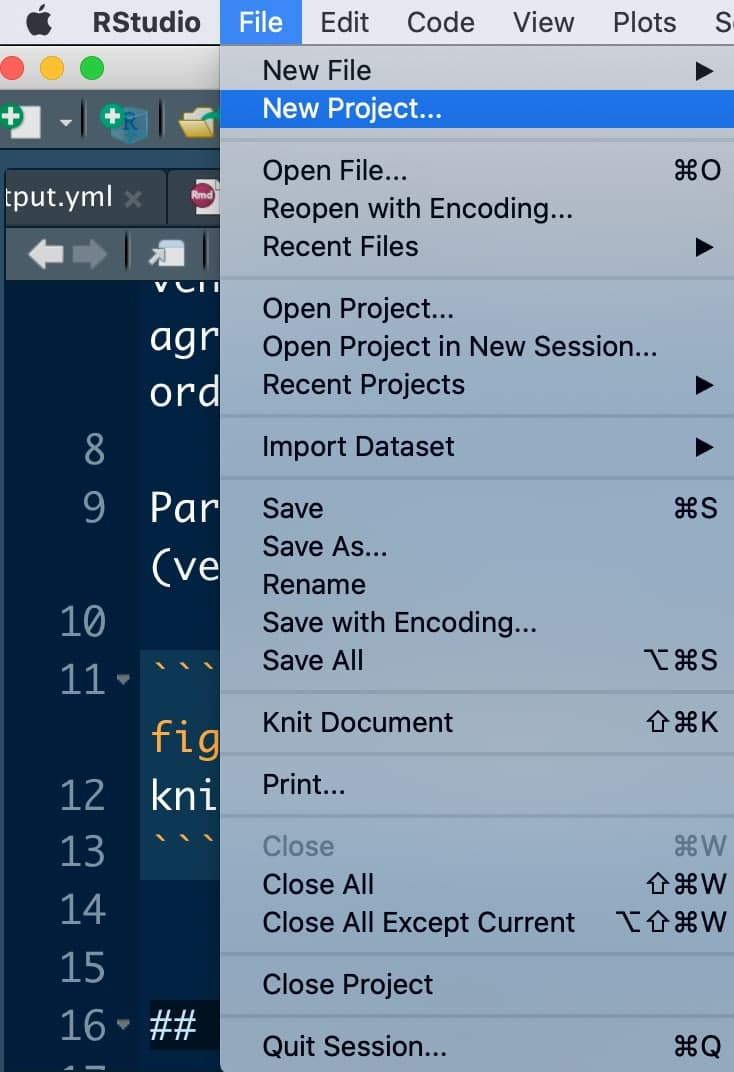
\includegraphics[width=0.5\linewidth]{./img/crear_proyecto1} 

}

\caption{Crear un nuevo proyecto en R.}\label{fig:crear-proyecto1}
\end{figure}

Se nos abrirá una ventana con 3 opciones:

\begin{itemize}
\item
  \textbf{New directory}: crear un proyecto desde el inicio (\textbf{opción recomendable}).
\item
  \textbf{Existing directory}: crear un proyecto con los códigos que tienes ya guardados en una carpeta.
\item
  \textbf{Version control}: para importar el proyecto de algún repositorio y vincularlo a él.
\end{itemize}

\begin{figure}

{\centering 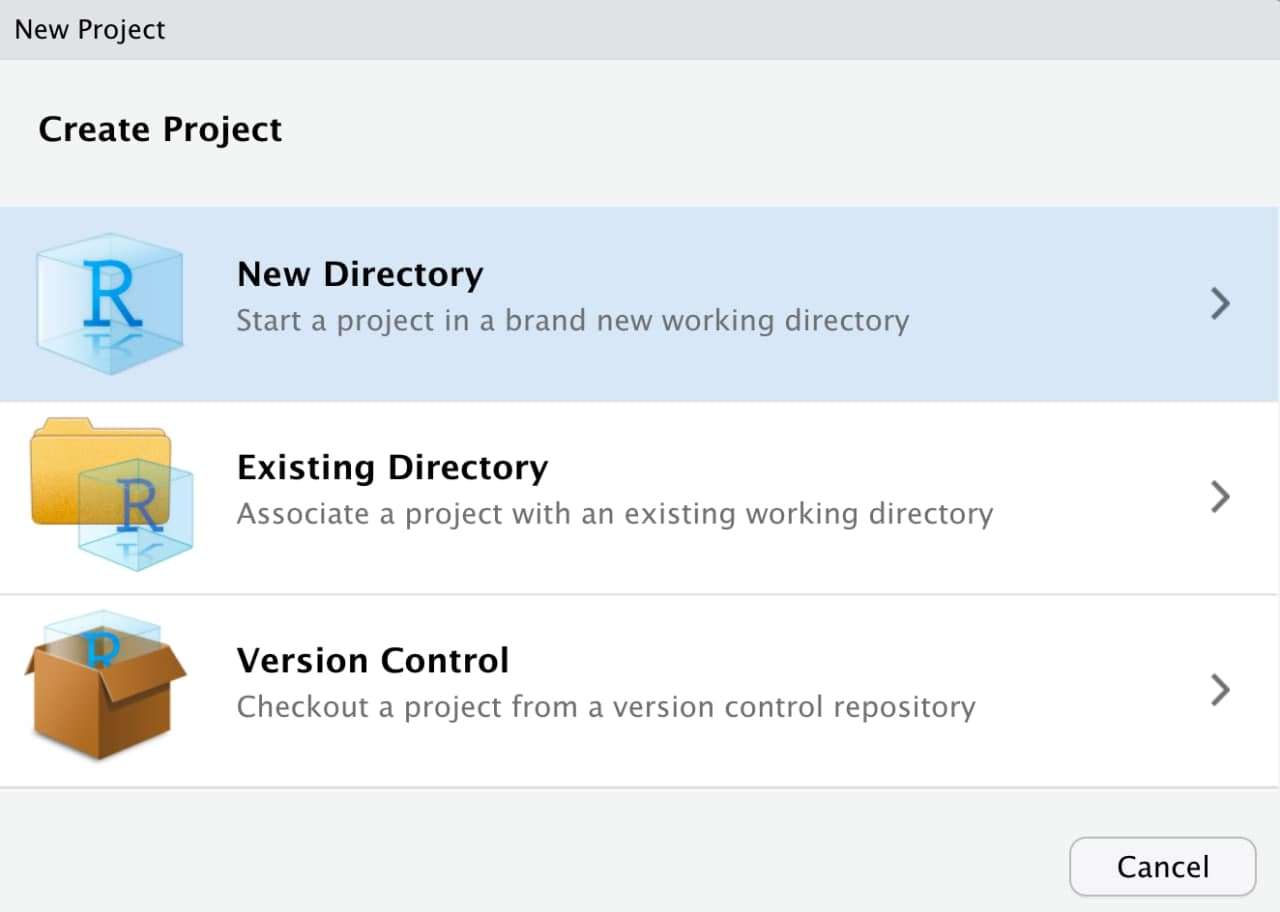
\includegraphics[width=0.5\linewidth]{./img/crear_proyecto2} 

}

\caption{Opciones de creación.}\label{fig:crear-proyecto2}
\end{figure}

\begin{figure}

{\centering 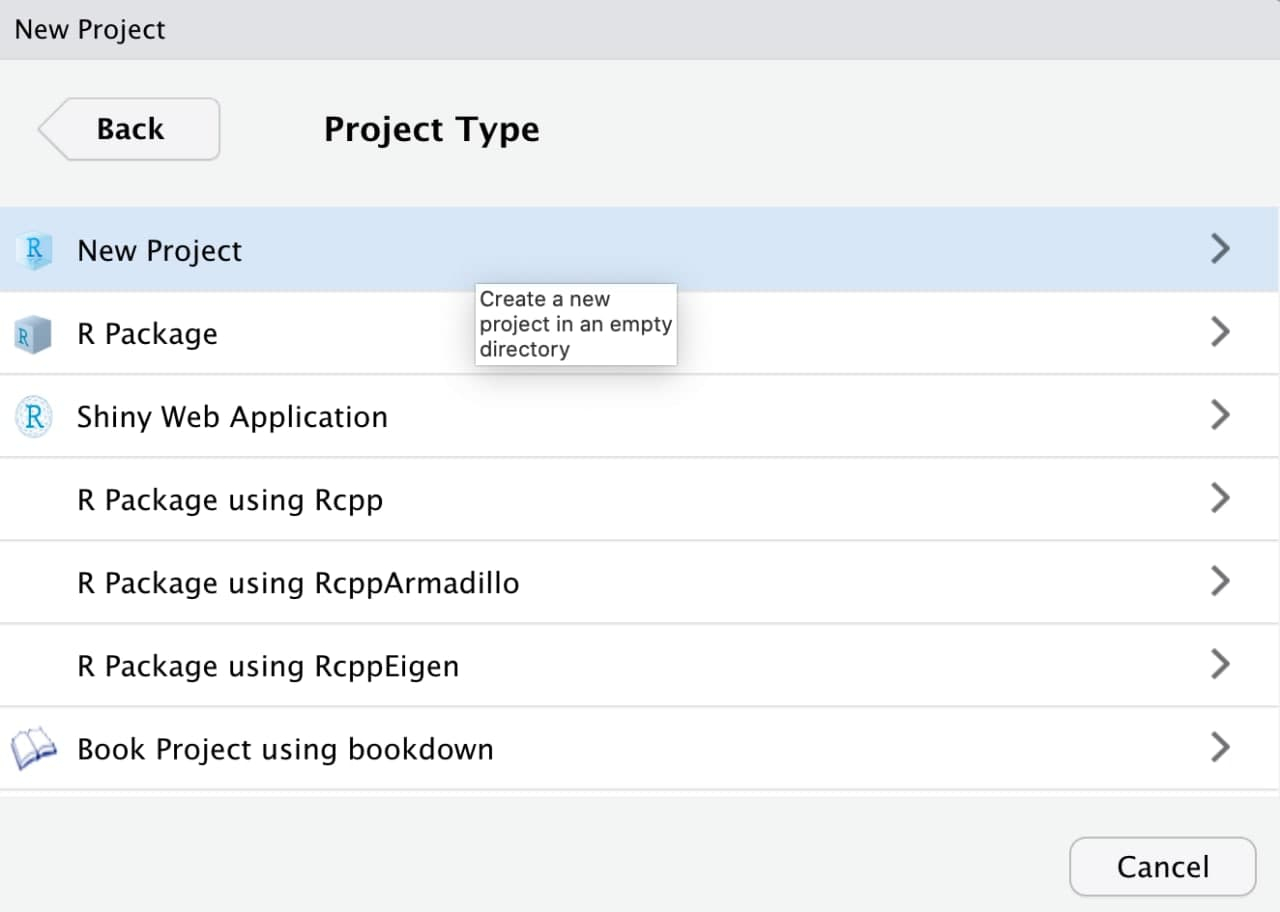
\includegraphics[width=0.5\linewidth]{./img/crear_proyecto3} 

}

\caption{Clickar en «New project».}\label{fig:crear-proyecto3}
\end{figure}

Deberemos elegir el \textbf{directorio de nuestro ordenador} donde queremos que se guarde (una carpeta que contendrá todos los códigos y datos de ese proyecto), así como el \textbf{nombre del proyecto} (que será a su vez el nombre de la subcarpeta que se os creará en el ordenador).

\begin{figure}

{\centering 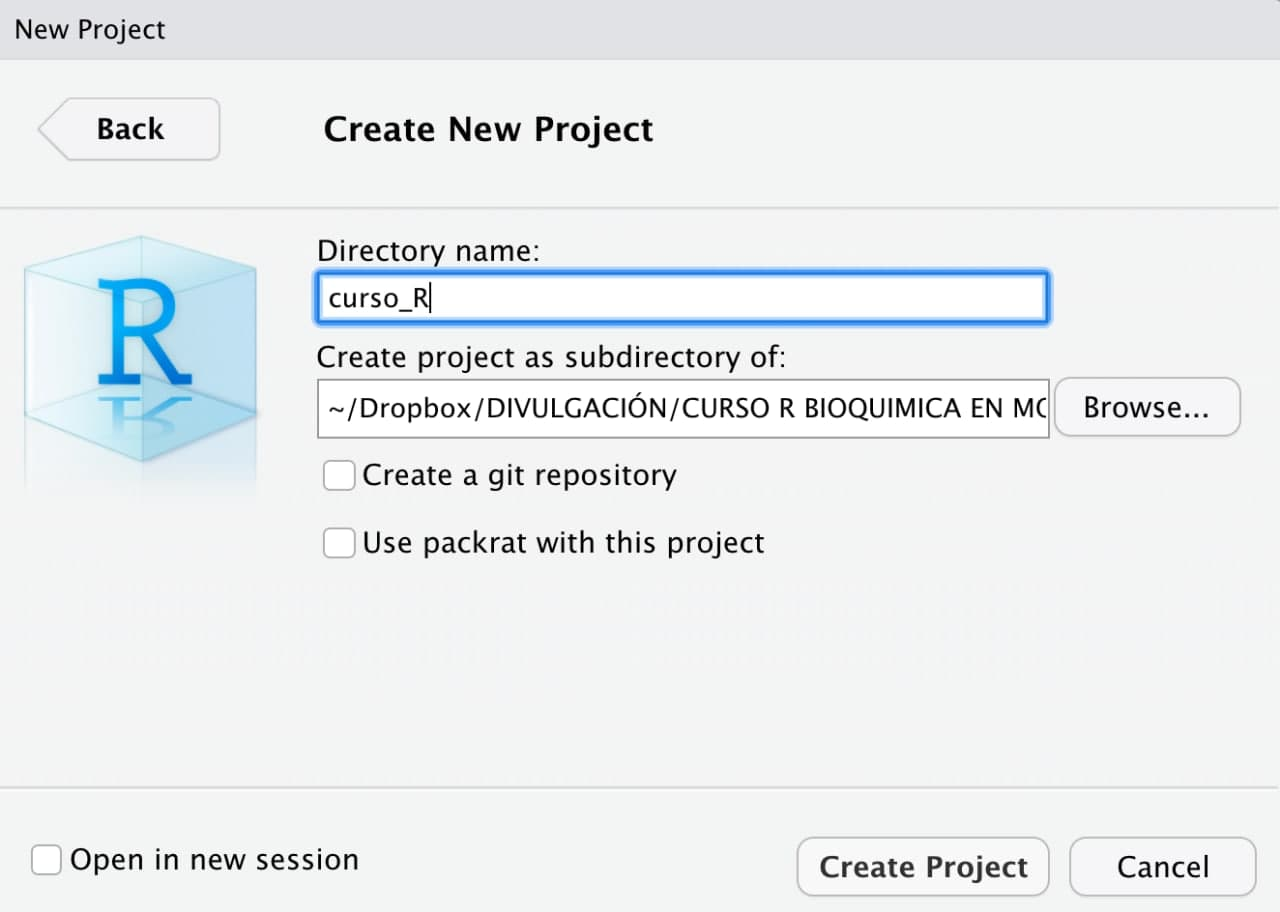
\includegraphics[width=0.5\linewidth]{./img/crear_proyecto4} 

}

\caption{Nombre del proyecto.}\label{fig:crear-proyecto4}
\end{figure}

Una vez que el proyecto está creado, abriremos nuestro primer \textbf{script de \texttt{R}} (donde escribiremos el código), escribiremos una descripción del proyecto en la primera línea y guardaremos el archivo (archivo de extensión \texttt{.R}).

\begin{figure}

{\centering 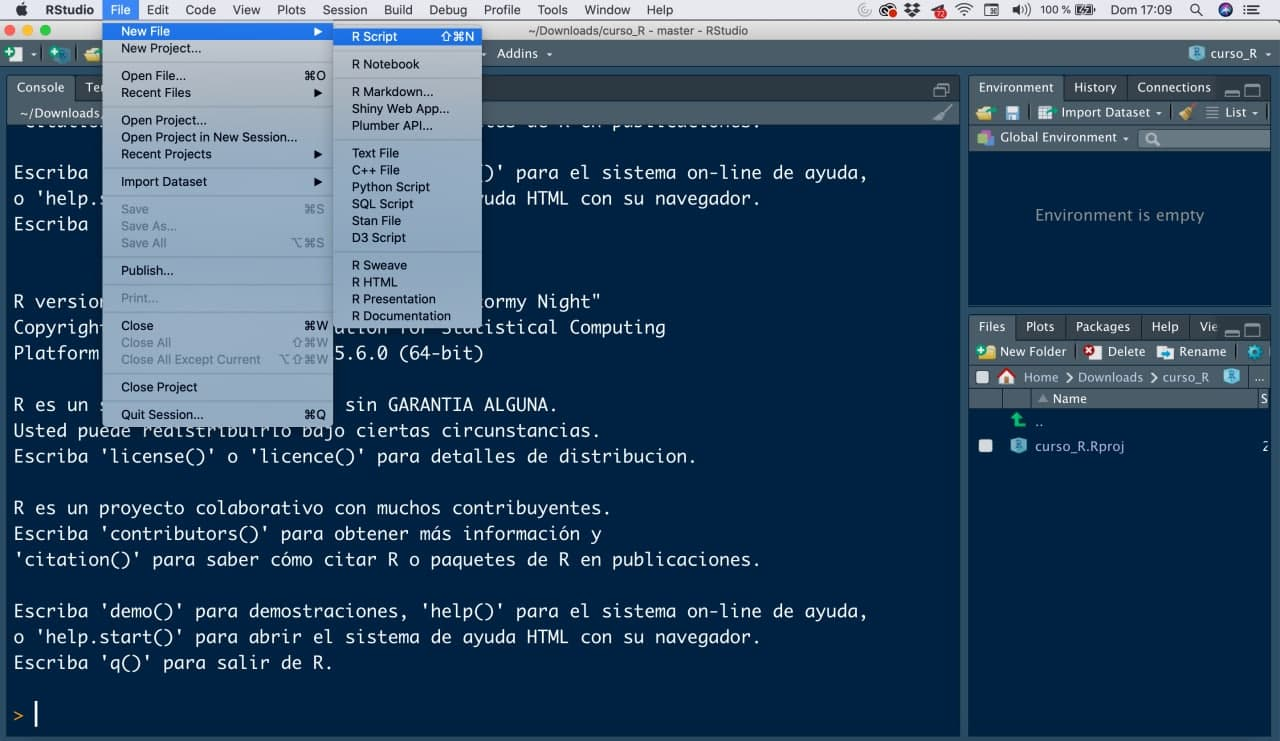
\includegraphics[width=0.5\linewidth]{./img/crear_proyecto5} 

}

\caption{Abrir nuestro primer script de R.}\label{fig:crear-proyecto5}
\end{figure}

\begin{figure}

{\centering 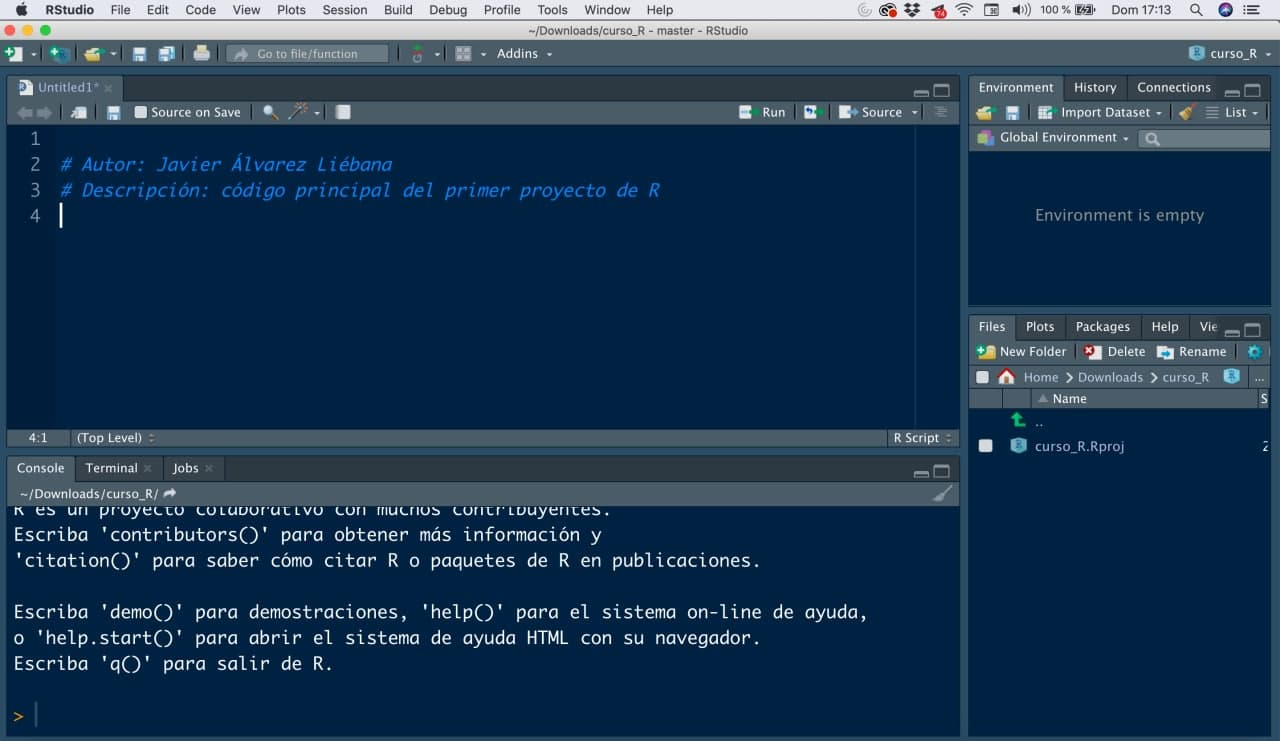
\includegraphics[width=0.5\linewidth]{./img/crear_proyecto6} 

}

\caption{Descripción al inicio del código.}\label{fig:crear-proyecto6}
\end{figure}

\begin{figure}

{\centering 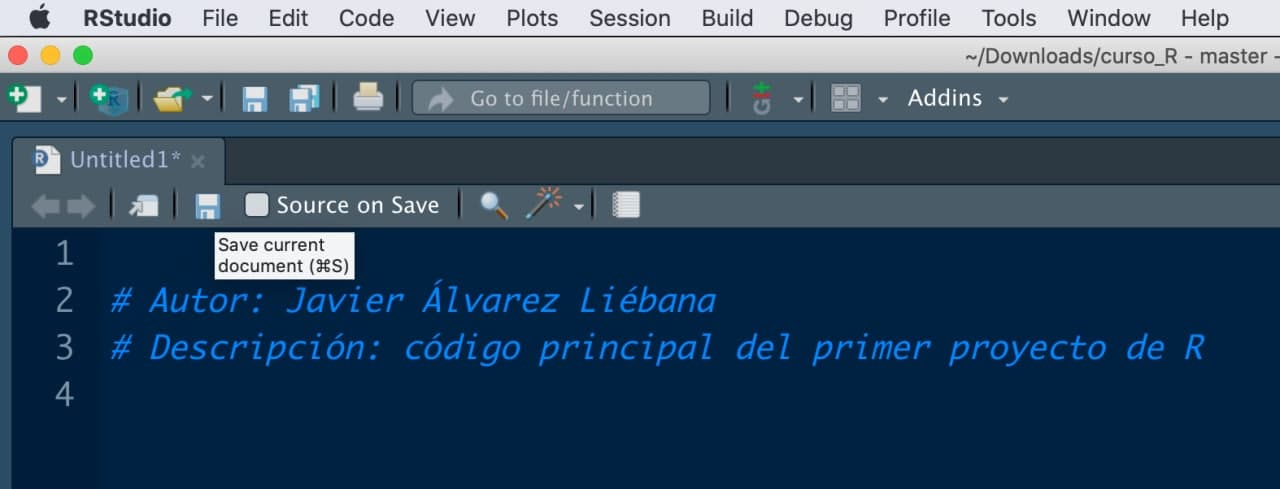
\includegraphics[width=0.5\linewidth]{./img/crear_proyecto7} 

}

\caption{Guardamos el código.}\label{fig:crear-proyecto7}
\end{figure}

\begin{figure}

{\centering 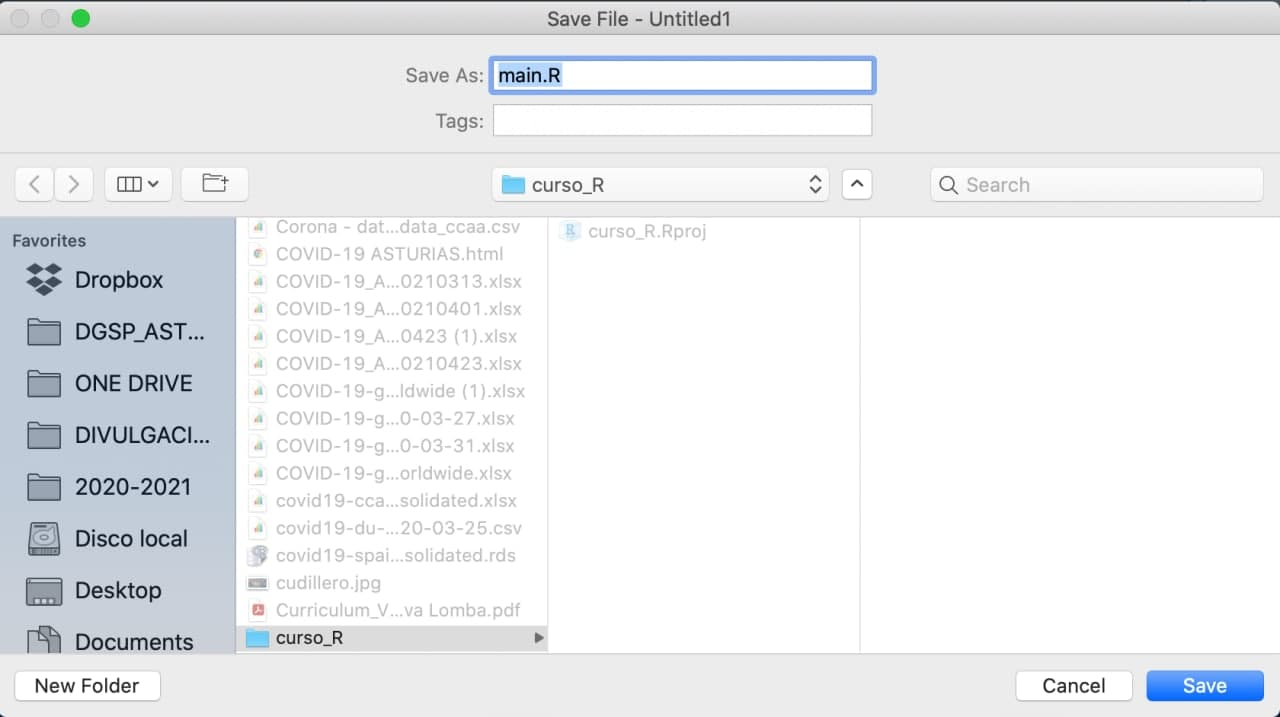
\includegraphics[width=0.5\linewidth]{./img/crear_proyecto8} 

}

\caption{Guardamos el código.}\label{fig:crear-proyecto8}
\end{figure}

Este será nuestro \textbf{código principal} (puedes ponerle el nombre que quieras, normalmente se le llama \texttt{main.R} para diferenciarlo del resto), desde el que iremos construyendo nuestro código e iremos llamando a otros archivos si es necesario. Recuerda que \textbf{programar es como escribir}: cuanto más limpio y estructurado, mejor se entenderá.

~

La \textbf{ventaja de tener los códigos agrupados por proyectos} es que si estamos trabajando en varios a la vez podemos saltar de uno a otro, visualizando solo los códigos de un proyecto, y no los 100 archivos \texttt{sin\_titulo131.R} que vayamos creando.

\begin{figure}

{\centering 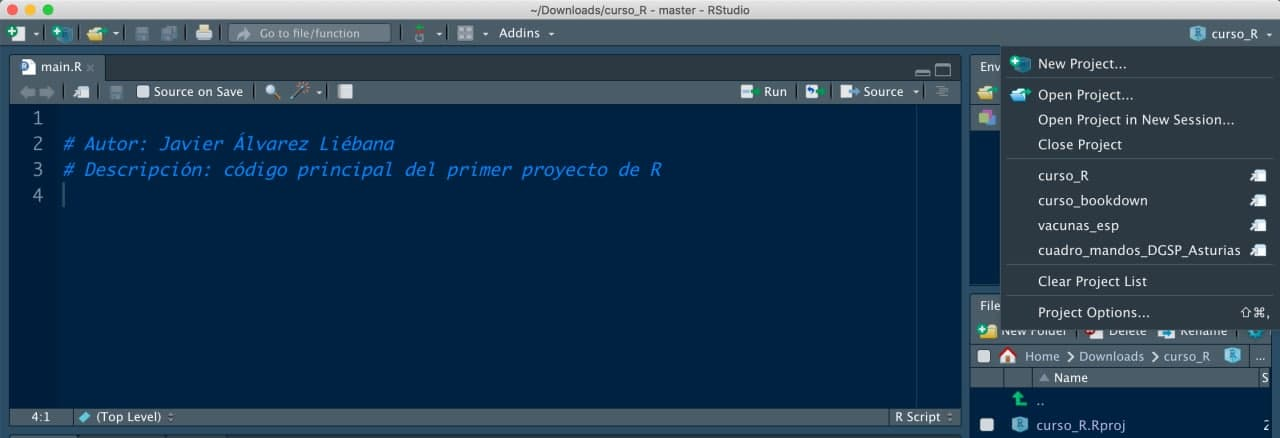
\includegraphics[width=0.5\linewidth]{./img/crear_proyecto9} 

}

\caption{Saltar de proyecto en proyecto.}\label{fig:crear-proyecto9}
\end{figure}

\hypertarget{directorios-de-trabajo-y-cabecera}{%
\section{Directorios de trabajo y cabecera}\label{directorios-de-trabajo-y-cabecera}}

Como luego veremos en la \ref{datos}, es altamente recomendable que \textbf{todos los archivos (códigos, datos, imágenes, recursos, etc)} los tengamos dentro de la misma carpeta del proyecto (aunque podamos crear subdirectorios), para que trabajar en el proyecto sea más sencillo e intuitivo. Vamos a crearnos dentro de la carpeta del proyecto, una subcarpeta que se llame \texttt{CODIGOS}, y creamos un script llamado \texttt{variables.R} dentro de esa carpeta.

\begin{figure}

{\centering 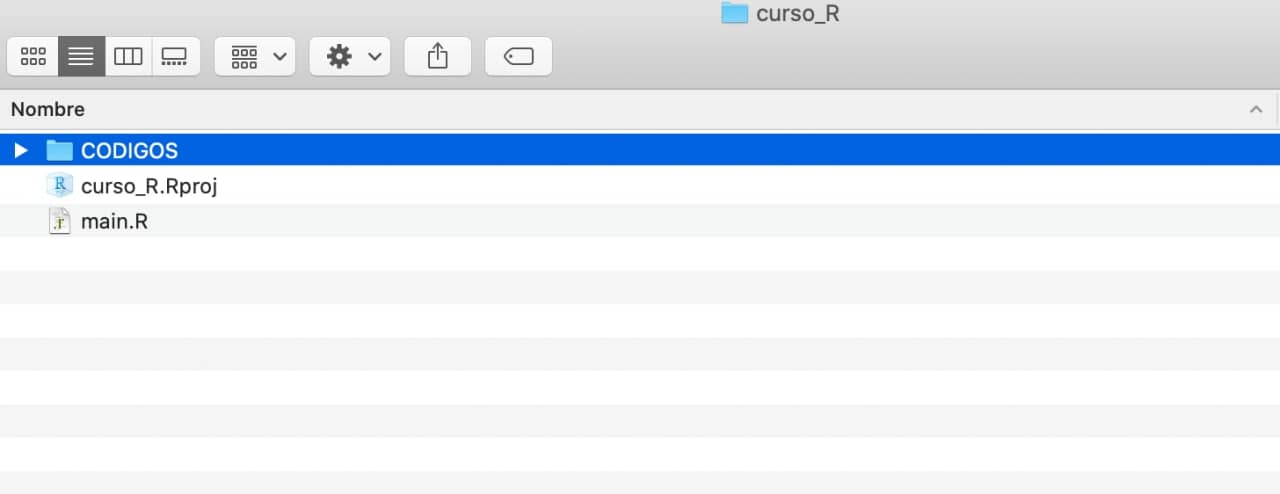
\includegraphics[width=0.5\linewidth]{./img/carpeta_codigos} 

}

\caption{Subcarpeta «CODIGOS».}\label{fig:carpeta-codigos}
\end{figure}

\begin{figure}

{\centering 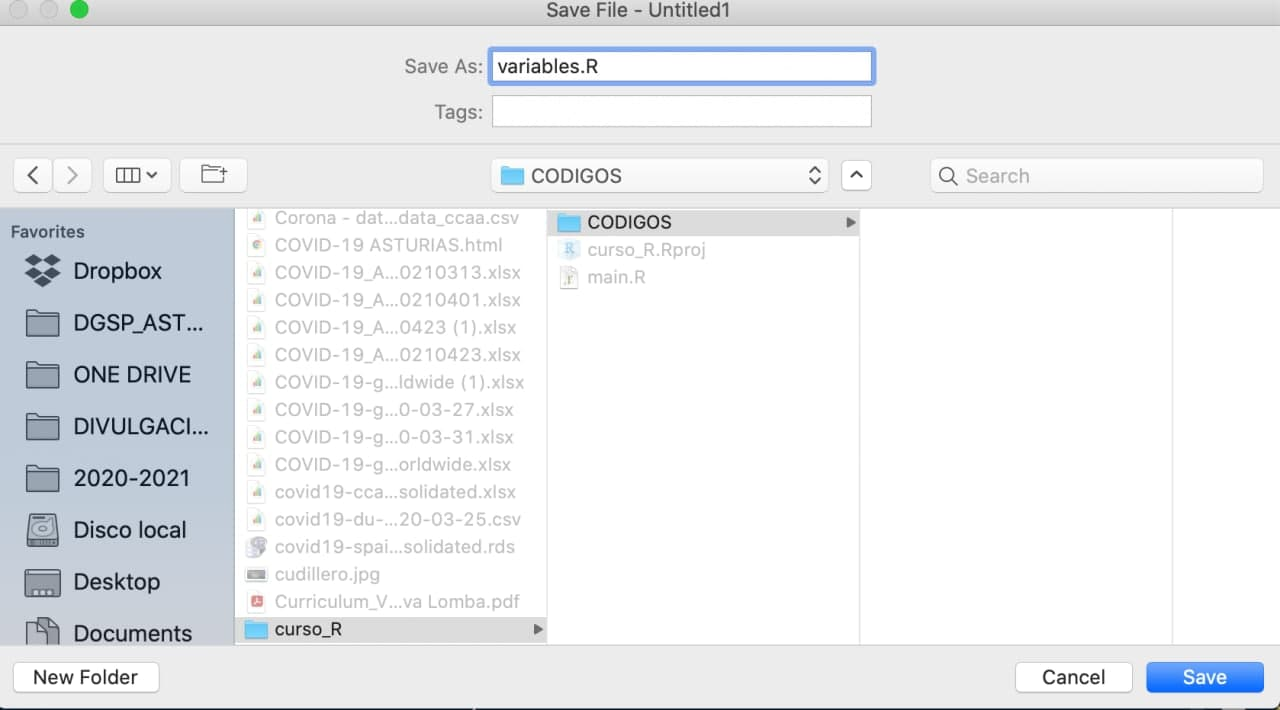
\includegraphics[width=0.5\linewidth]{./img/carpeta_codigos1} 

}

\caption{Creamos un fichero «variables.R».}\label{fig:carpeta-codigos1}
\end{figure}

En ese código de prueba vamos a \textbf{definir algunas variables fijas} que luego usaremos en el código principal (suele suceder con variables que van a ser fijas como nombres, fechas o codificaciones de variables).

\begin{Shaded}
\begin{Highlighting}[]
\CommentTok{# Descripción: script de prueba con variables}

\CommentTok{# Variables}
\NormalTok{x <-}\StringTok{ }\KeywordTok{c}\NormalTok{(}\DecValTok{1}\NormalTok{, }\DecValTok{2}\NormalTok{, }\DecValTok{0}\NormalTok{, }\DecValTok{-1}\NormalTok{, }\DecValTok{71}\NormalTok{) }\CommentTok{# Vector de números}
\NormalTok{y <-}\StringTok{ }\KeywordTok{c}\NormalTok{(}\StringTok{"hola"}\NormalTok{, }\StringTok{"me"}\NormalTok{, }\StringTok{"llamo"}\NormalTok{, }\StringTok{"Javier"}\NormalTok{) }\CommentTok{# Vector de caracteres}
\NormalTok{apellido <-}\StringTok{ "Álvarez"}

\CommentTok{# Fechas}
\NormalTok{hoy <-}\StringTok{ }\KeywordTok{as.Date}\NormalTok{(}\KeywordTok{Sys.time}\NormalTok{()) }\CommentTok{# Convertir a tipo fecha la fecha de hoy}
\NormalTok{fecha_origen <-}\StringTok{ }\KeywordTok{as.Date}\NormalTok{(}\StringTok{"2021-01-01"}\NormalTok{) }\CommentTok{# Inicio de año}
\end{Highlighting}
\end{Shaded}

\begin{figure}

{\centering 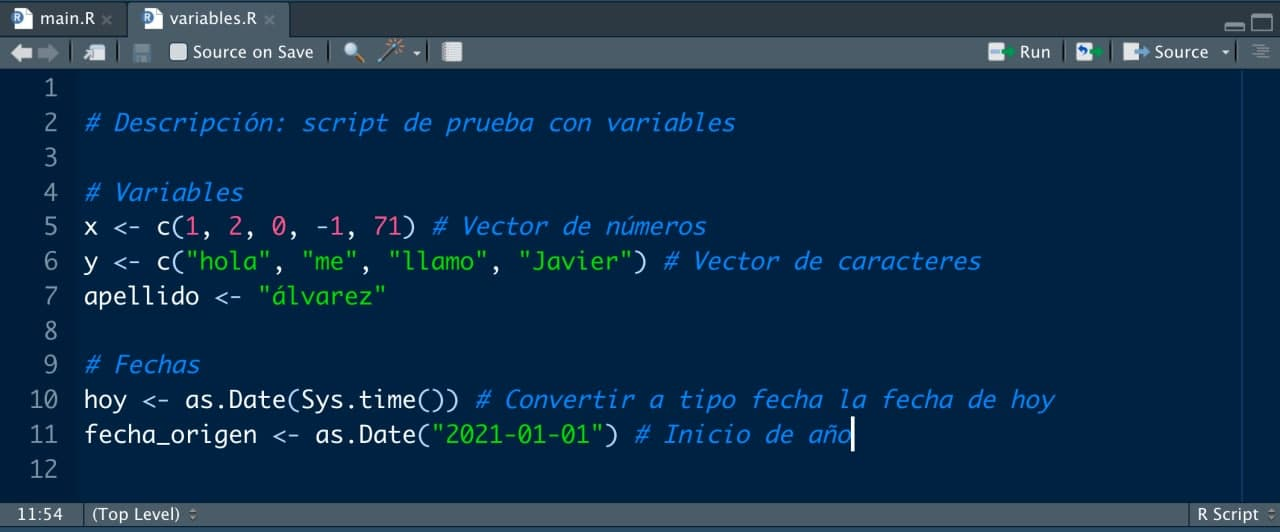
\includegraphics[width=0.5\linewidth]{./img/carpeta_codigos2} 

}

\caption{Escribimos una serie de variables fijas para luego ser usadas.}\label{fig:carpeta-codigos2}
\end{figure}

No es obligatorio pero es \textbf{altamente recomendable} tener muy estructurado nuestros códigos, de forma que el archivo \texttt{.R} haga una \textbf{tarea concreta y definida} (uno carga archivos, otro preprocesa, otro hace un modelo, otro hace las gráficas), y sea el \textbf{código principal el que haga una llamada limpia a todos ellos}, para que en caso de error, la detección del mismo sea más sencilla.

Así que eso haremos: desde nuestro archivo principal \texttt{main.R} llamaremos a ese archivo \texttt{variables.R}, para luego usar las variables definidas en él.

\textbf{¿Cómo indicarle a \texttt{R} donde está nuestro fichero?}

En \texttt{R}, como en todo lenguaje de programación, podemos consultar lo que el ordenador llama \emph{directorio de trabajo}: la carpeta «base» desde donde está ejecutando tu código. Dicha ruta de directorio se puede consultar con la función \texttt{getwd()}, pudiendo ver los archivos y carpetas que hay dentro del mismo con el comando \texttt{dir()}

\begin{Shaded}
\begin{Highlighting}[]
\KeywordTok{getwd}\NormalTok{()}
\KeywordTok{dir}\NormalTok{()}
\end{Highlighting}
\end{Shaded}

\begin{figure}

{\centering 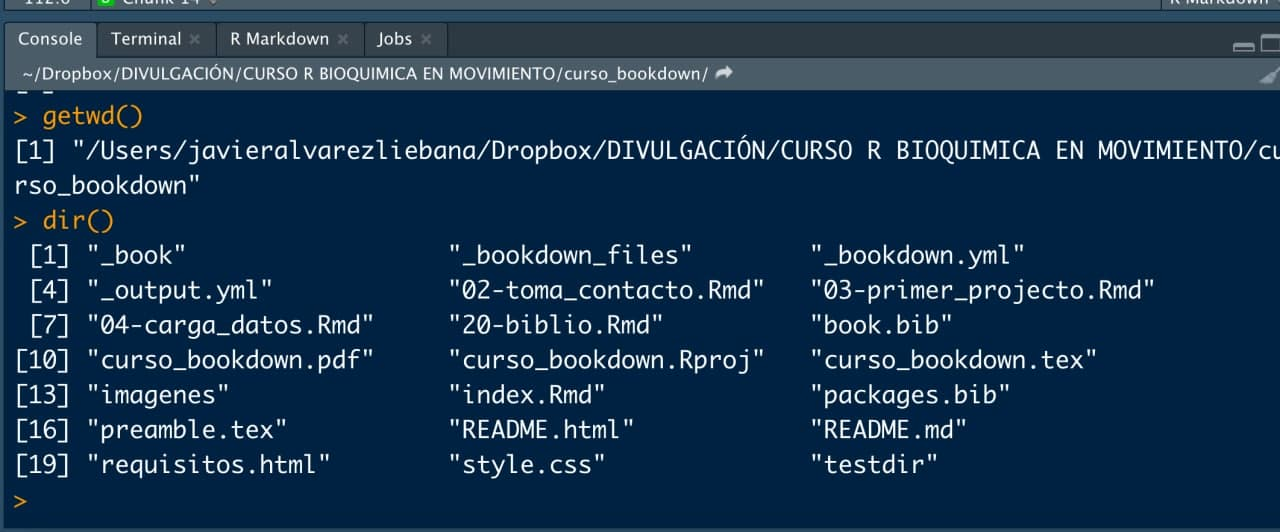
\includegraphics[width=0.5\linewidth]{./img/getwd} 

}

\caption{Consultar directorio de trabajo predeterminado y archivos contenidos en él.}\label{fig:getwd}
\end{figure}

Lo ideal es empezar el código \textbf{fijando como directorio de trabajo el directorio donde tengamos nuestro archivo principal} \texttt{main.R} y para ello usaremos la función \texttt{setwd()}, cuyo argumento será la ruta donde queremos fijarlo. Para hacerlo de forma automática (y que el código pueda ser abierto por ti pero también por otros que no tengan tu misma estructura de carpetas), obtendremos de forma automática la ruta del archivo \texttt{main.R} o del proyecto con la orden \texttt{rstudioapi::getSourceEditorContext()\$path}, y después usaremos \texttt{dirname()} para quedarnos solo con la ruta de carpetas (eliminando el nombre del fichero al final). Esa será la ruta que le pasaremos a \texttt{setwd()}, quedando nuestro directorio de trabajo automáticamente fijado, sin preocuparnos de la ruta

\begin{Shaded}
\begin{Highlighting}[]
\CommentTok{# Fijamos directorio de trabajo automáticamente}
\KeywordTok{setwd}\NormalTok{(}\KeywordTok{dirname}\NormalTok{(rstudioapi}\OperatorTok{::}\KeywordTok{getSourceEditorContext}\NormalTok{()}\OperatorTok{$}\NormalTok{path))}
\end{Highlighting}
\end{Shaded}

\begin{figure}

{\centering 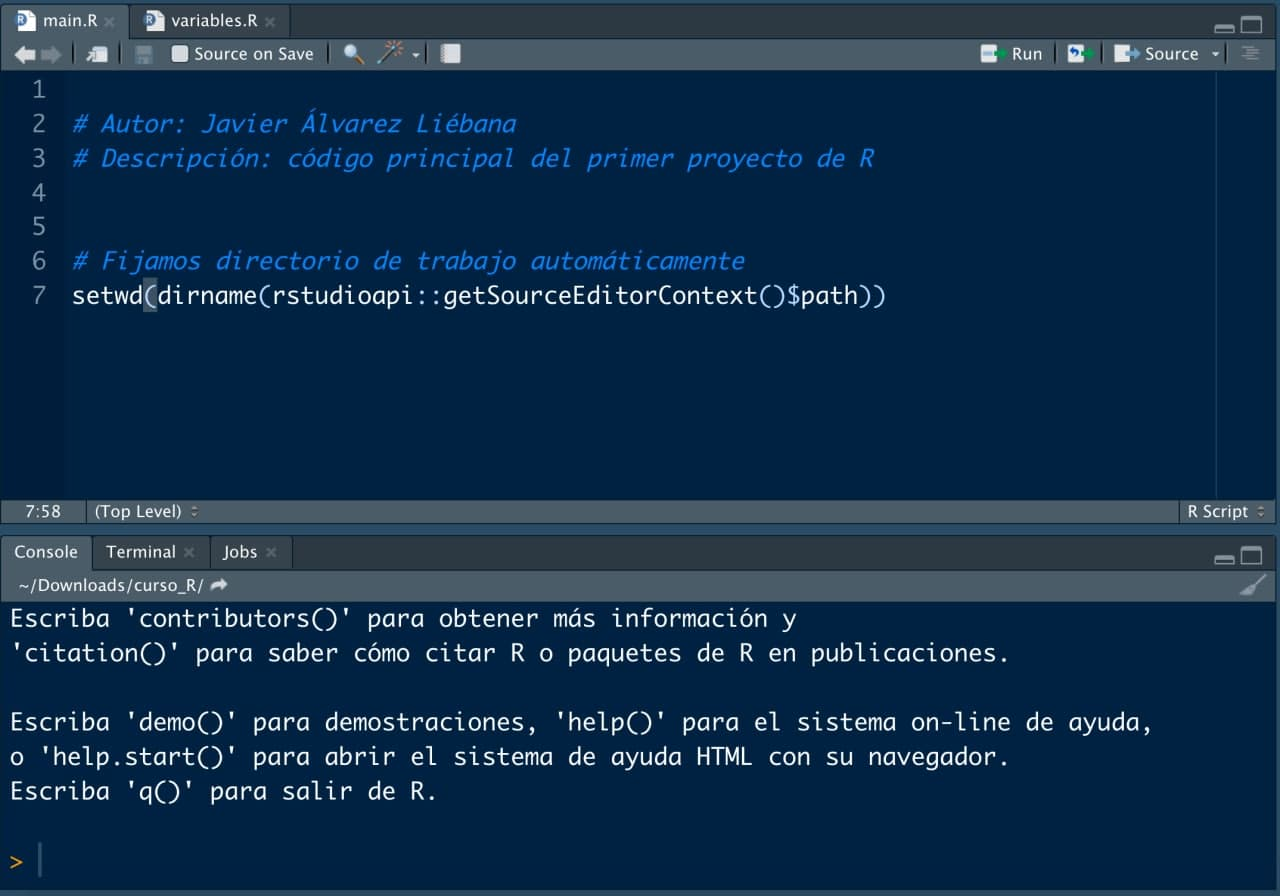
\includegraphics[width=0.5\linewidth]{./img/setwd} 

}

\caption{Fijamos de forma automático el directorio de trabajo.}\label{fig:setwd}
\end{figure}

Una vez que hemos fijado nuestro directorio, para cargar código \texttt{.R}, basta que usemos la función \texttt{source()}, cuyo argumento será la ruta del archivo. Como tenemos de directorio base el directorio en el que tenemos nuestro archivo principal (\texttt{./}), bastará que empecemos a escribir \texttt{source("./")}, presionar el tabulador, y se nos abrirá el menú de archivos de nuestro directorio de trabajo, pudiendo ir seleccionando de forma sencilla la ruta de nuestro archivo.

\begin{Shaded}
\begin{Highlighting}[]
\CommentTok{# Cargamos fichero variable.R}
\KeywordTok{source}\NormalTok{(}\StringTok{"./CODIGOS/variables.R"}\NormalTok{)}
\end{Highlighting}
\end{Shaded}

\begin{figure}

{\centering 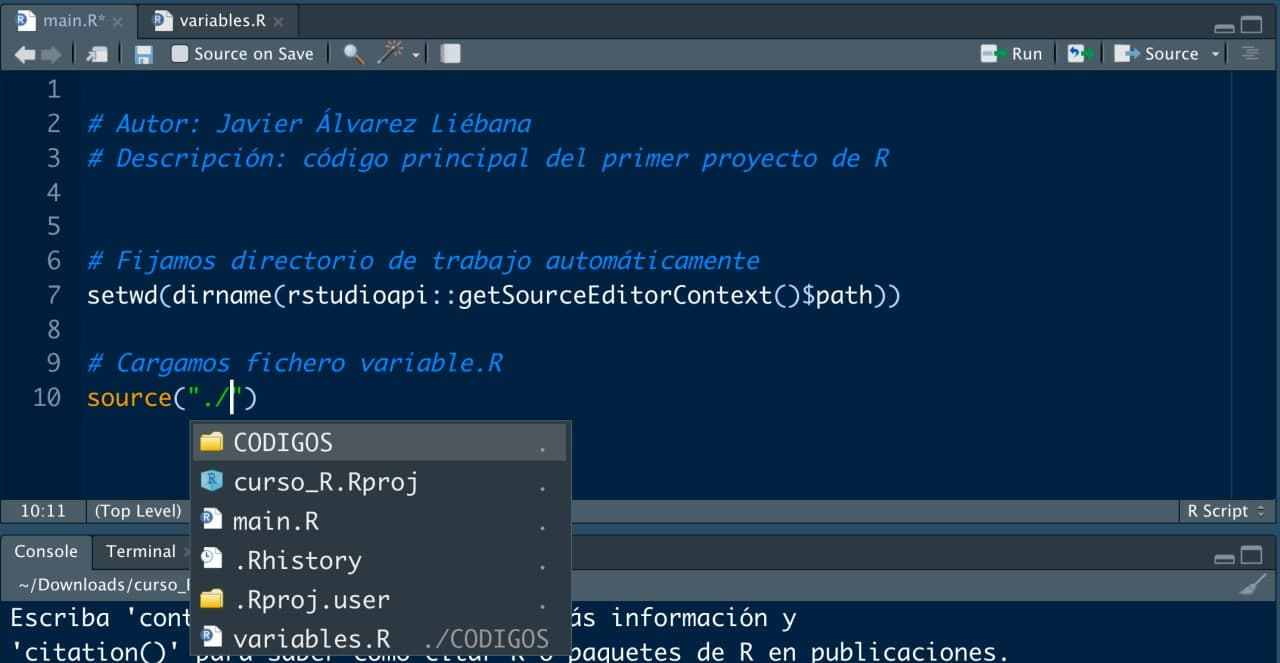
\includegraphics[width=0.5\linewidth]{./img/menu_carpetas} 

}

\caption{Cargar archivos de nuestro directorio de trabajo.}\label{fig:menu-carpetas}
\end{figure}

\begin{figure}

{\centering 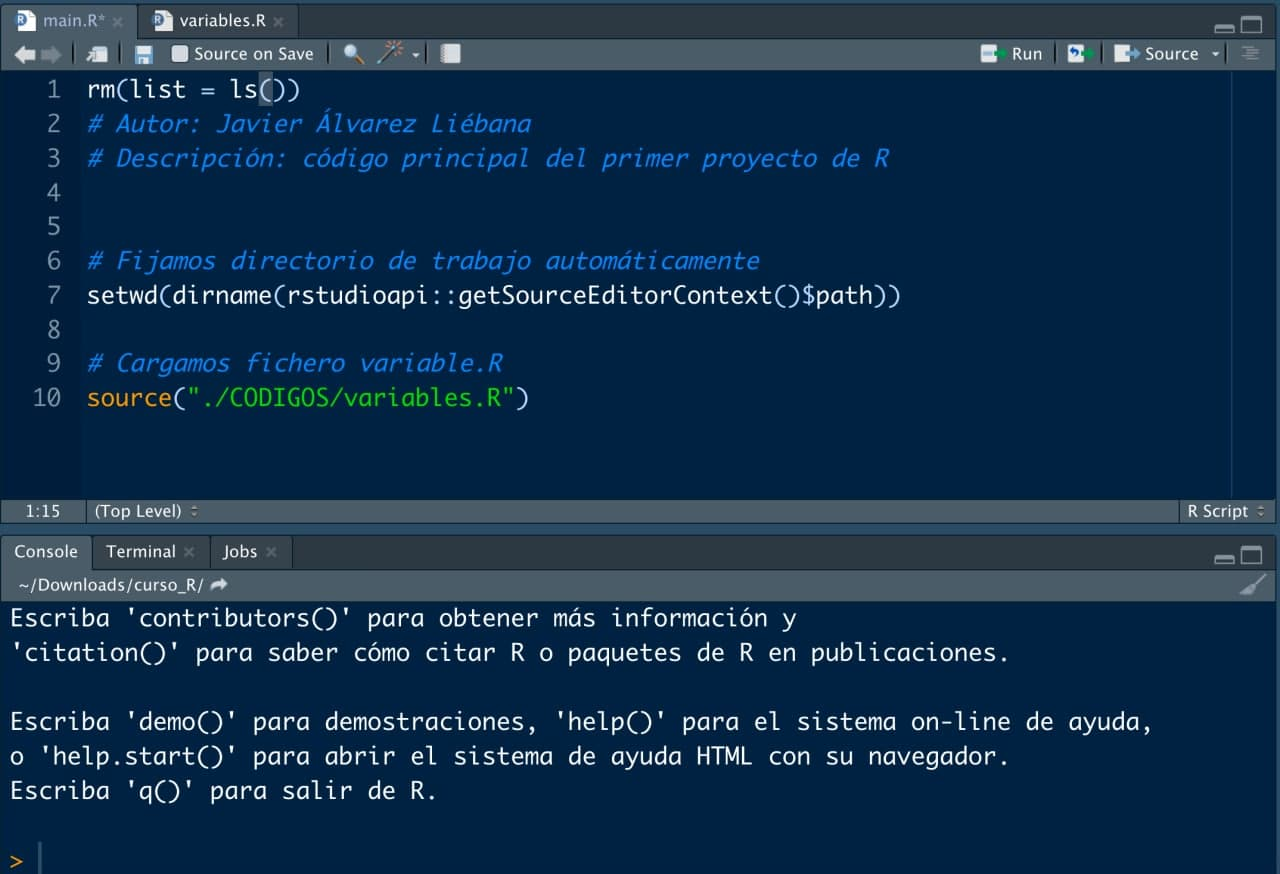
\includegraphics[width=0.5\linewidth]{./img/menu_carpetas1} 

}

\caption{Cargar archivos de nuestro directorio de trabajo.}\label{fig:menu-carpetas1}
\end{figure}

\hypertarget{ejecuciuxf3n}{%
\section{Ejecución}\label{ejecuciuxf3n}}

Ese archivo que hemos incluido en el código principal nos \textbf{cargará las variables que hemos definido en él}, pudiendo usarlas en el código. Vamos a ejecutar lo que tenemos de momento, y para ello tenemos 2 opciones: o copiar el código del script en la consola y pulsar \emph{ENTER}, o bien, activando la casilla \emph{source on save} y guardando el script (no solo se guardará sino que se ejecutará).

\begin{figure}

{\centering \includegraphics[width=0.5\linewidth]{./img/source_on_save} 

}

\caption{Guardamos con la casilla «source on save» activada para que además de guardar se ejecute el código.}\label{fig:source-on-save}
\end{figure}

Como vemos en la imagen \ref{fig:source-on-save}, una vez ejecutado, tenemos en nuestro panel de entorno (parte superior derecha) las variables ya cargadas que teníamos definidas en nuestro fichero \texttt{variables.R}.

Prueba a escribir algunas funciones que hemos aprendido con dichas variables y vuelve a hacer click en «guardar» con \emph{source on save} activado.

\begin{Shaded}
\begin{Highlighting}[]
\CommentTok{# Sumamos 3 a cada elemento de x}
\NormalTok{z <-}\StringTok{ }\NormalTok{x }\OperatorTok{+}\StringTok{ }\DecValTok{3}
\NormalTok{z}
\end{Highlighting}
\end{Shaded}

\begin{verbatim}
## [1]  4  5  3  2 74
\end{verbatim}

\begin{Shaded}
\begin{Highlighting}[]
\CommentTok{# Imprimimos por pantalla la frase unida, y a dicha frase}
\CommentTok{# le pegamos nuestro apellido}
\KeywordTok{cat}\NormalTok{(}\KeywordTok{paste}\NormalTok{(}\KeywordTok{paste}\NormalTok{(y, }\DataTypeTok{collapse =} \StringTok{" "}\NormalTok{), apellido))}
\end{Highlighting}
\end{Shaded}

\begin{verbatim}
## hola me llamo Javier Álvarez
\end{verbatim}

\begin{Shaded}
\begin{Highlighting}[]
\CommentTok{# Días que han pasado desde el inicio de año}
\NormalTok{dias <-}\StringTok{ }\NormalTok{hoy }\OperatorTok{-}\StringTok{ }\NormalTok{fecha_origen}
\NormalTok{dias}
\end{Highlighting}
\end{Shaded}

\begin{verbatim}
## Time difference of 247 days
\end{verbatim}

La función \texttt{cat()} nos muestra por consola el texto que le pasemos de argumento (\textbf{función especial para mensajes de alerta} por consola)

\begin{figure}

{\centering \includegraphics[width=0.5\linewidth]{./img/codigo_1} 

}

\caption{Cálculos con la variables definidas: suma, concatenación de texto y diferencia de fechas.}\label{fig:codigo-1}
\end{figure}

Ya hemos ejecutado nuestro primer proyecto en \texttt{.R} :)

\hypertarget{consejos-y-tips-3}{%
\section[ Consejos y tips]{\texorpdfstring{\protect\includegraphics[width=0.04\textwidth,height=\textheight]{img/logo_info.png} Consejos y tips}{ Consejos y tips}}\label{consejos-y-tips-3}}

Comentarios en los códigos

Es crucial que intentes \textbf{documentar al máximo tu código} y que te acostumbres a ello desde el principio, dejando explícito que haces en cada paso, tanto para ti como para otra persona que pueda leer tu código y lo entienda. Para ello usaremos \texttt{\#\ comentario} cuando queramos dejar comentarios en el código. Dichas partes, amén de estar en otro color, no son leídas por \texttt{R} ni ejecutadas: son comentarios que el programa «no ve», solo son para nosotros.

~

Limpiar el entorno

A veces empezamos a programar sin apagar el ordenador y tenemos variables guardadas de otros días que pueden generar conflictos y consumo de memoria. Para asegurarnos que cada vez que empezamos, lo hacemos de cero, es altamente recomendable empezar el código con \texttt{rm(list\ =\ ls())}. La función \texttt{ls()} nos devuelve todas las variables que tenemos definidas en nuestro entorno, y la función \texttt{rm()} nos las elimina.

~

Anular warnings

Algunas funciones pueden arrojarse ciertas advertencias que nunca está de más leer. Pero si dichos mensajes de alerta los tenemos controlados y no queremos que nos ensucie la ejecución en la consola, podemos poner al inicio del código \texttt{assign("last.warning",\ NULL,\ envir\ =\ baseenv())} para limpiar los warnings antiguos y \texttt{options(warn\ =\ -1)} para desactivarlos.

~

Limpiar consola

Podemos limpiar la consola clickando en al escoba que tenemos en la parte superior derecha de la misma. Esta acción \textbf{no nos elimina ninguna variable}, simplemente nos limpia la consola de mensajes.

~

Guardar los scripts

Los scripts que tengas sin guardar tendrán un asterisco \texttt{*} al final del nombre en la pestaña superior de la ventana.

~

Fecha y hora de hoy

La función \texttt{Sys.time()} accede al sistema de nuestro ordenador para decirnos la \textbf{fecha y hora del momento de la ejecución} de dicha función.

\begin{Shaded}
\begin{Highlighting}[]
\KeywordTok{Sys.time}\NormalTok{()}
\end{Highlighting}
\end{Shaded}

\begin{verbatim}
## [1] "2021-09-05 14:32:21 CEST"
\end{verbatim}

~

Cambiar la notación exponencial

Por defecto, \texttt{R} muestra los números en formato de notación exponencial. Por ejemplo, el número \texttt{1000000} nos lo mostrará por defecto como \texttt{1e+06}. A veces podemos querer que se muestre con todas sus cifras (por ejemplo, en el título o leyenda de una gráfica): para anular la notación exponencial, escribe al inicio del código \texttt{options("scipen"\ =\ 10)}.

\hypertarget{datos}{%
\chapter{Tipos de datos II: tablas}\label{datos}}

Sabemos un poco de la gramática y ortografía de nuestro lenguaje, y sabemos las funcionalidades básicas de nuestro Word. Vamos a encontrar la mejor trama para la novela: \textbf{hablemos de estructuras de datos}.

\hypertarget{matrices}{%
\section{Matrices}\label{matrices}}

Hasta ahora \textbf{hemos visto solo datos en una dimensión}: una variable, que tiene n valores numéricos, n valores lógicos o n valores de tipo texto. \textbf{Una sola variable} (de n elementos).

Pero cuando analizamos datos solemos tener varias variables distintas. Cuando tenemos \textbf{distintas variables numéricas de igual longitud}, un formato de dato muy habitual de trabajar es lo que conocemos como \textbf{matrices}: una «tabla» de números, con filas y columnas.

Vamos a definir las \textbf{edades, teléfonos y códigos postales de una serie de individuos}.

\begin{Shaded}
\begin{Highlighting}[]
\NormalTok{edades <-}\StringTok{ }\KeywordTok{c}\NormalTok{(}\DecValTok{14}\NormalTok{, }\DecValTok{24}\NormalTok{, }\DecValTok{56}\NormalTok{, }\DecValTok{31}\NormalTok{, }\DecValTok{20}\NormalTok{, }\DecValTok{87}\NormalTok{, }\DecValTok{73}\NormalTok{) }\CommentTok{# vector numérico de longitud 7}
\NormalTok{tlf <-}\StringTok{ }\KeywordTok{c}\NormalTok{(}\OtherTok{NA}\NormalTok{, }\DecValTok{683839390}\NormalTok{, }\DecValTok{621539732}\NormalTok{, }\DecValTok{618211286}\NormalTok{, }\OtherTok{NA}\NormalTok{, }\DecValTok{914727164}\NormalTok{, }\OtherTok{NA}\NormalTok{)}
\NormalTok{cp <-}\StringTok{ }\KeywordTok{c}\NormalTok{(}\DecValTok{33007}\NormalTok{, }\DecValTok{28019}\NormalTok{, }\DecValTok{37005}\NormalTok{, }\DecValTok{18003}\NormalTok{, }\DecValTok{33091}\NormalTok{, }\DecValTok{25073}\NormalTok{, }\DecValTok{17140}\NormalTok{)}
\end{Highlighting}
\end{Shaded}

Hasta ahora, cada variable la hemos definido por separado, pero ahora vamos a juntarlas: vamos a crear nuestro \textbf{primer conjunto de datos} juntado todas ellas en una matriz, un conjunto de números organizado en \textbf{3 columnas (una por variable)} y \textbf{7 filas o registros (una por persona)}. Para ello usaremos la función \texttt{cbind()}, que nos concatena vectores de igual longitud en formato columna.

\begin{Shaded}
\begin{Highlighting}[]
\NormalTok{x <-}\StringTok{ }\KeywordTok{cbind}\NormalTok{(edades, tlf, cp) }\CommentTok{# Construimos la matriz por columnas}
\NormalTok{x}
\end{Highlighting}
\end{Shaded}

\begin{verbatim}
##      edades       tlf    cp
## [1,]     14        NA 33007
## [2,]     24 683839390 28019
## [3,]     56 621539732 37005
## [4,]     31 618211286 18003
## [5,]     20        NA 33091
## [6,]     87 914727164 25073
## [7,]     73        NA 17140
\end{verbatim}

Lo que tenemos es una columna por variable y una fila por registro. También podemos construir la matriz por filas con el comando \texttt{rbind()} (aunque lo habitual es tener cada variable en una columna).

\begin{Shaded}
\begin{Highlighting}[]
\NormalTok{y <-}\StringTok{ }\KeywordTok{rbind}\NormalTok{(edades, tlf, cp) }\CommentTok{# Construimos la matriz por filas}
\NormalTok{y}
\end{Highlighting}
\end{Shaded}

\begin{verbatim}
##         [,1]      [,2]      [,3]      [,4]  [,5]      [,6]  [,7]
## edades    14        24        56        31    20        87    73
## tlf       NA 683839390 621539732 618211286    NA 914727164    NA
## cp     33007     28019     37005     18003 33091     25073 17140
\end{verbatim}

Como ves, ahora nuestros datos están \textbf{tabulados}, tienen dos dimensiones. ¿Cómo saber las \textbf{dimensiones} que tiene una matriz? Prueba a ejecutar la función \texttt{dim()}.

\begin{Shaded}
\begin{Highlighting}[]
\KeywordTok{dim}\NormalTok{(x)}
\end{Highlighting}
\end{Shaded}

\begin{verbatim}
## [1] 7 3
\end{verbatim}

\begin{Shaded}
\begin{Highlighting}[]
\KeywordTok{dim}\NormalTok{(y)}
\end{Highlighting}
\end{Shaded}

\begin{verbatim}
## [1] 3 7
\end{verbatim}

Fíjate que \texttt{dim()} devuelve un vector de 2 elementos, por lo que para acceder las filas deberemos ejecutar \texttt{dim(x){[}1{]}} (y \texttt{dim(x){[}2{]}} para las columnas). También tenemos a nuestra disposición las funciones \texttt{nrow()} y \texttt{ncol()}, que nos devuelven directamente el número de filas y columnas.

\begin{Shaded}
\begin{Highlighting}[]
\KeywordTok{dim}\NormalTok{(x)[}\DecValTok{1}\NormalTok{]}
\end{Highlighting}
\end{Shaded}

\begin{verbatim}
## [1] 7
\end{verbatim}

\begin{Shaded}
\begin{Highlighting}[]
\KeywordTok{dim}\NormalTok{(x)[}\DecValTok{2}\NormalTok{]}
\end{Highlighting}
\end{Shaded}

\begin{verbatim}
## [1] 3
\end{verbatim}

\begin{Shaded}
\begin{Highlighting}[]
\KeywordTok{nrow}\NormalTok{(x)}
\end{Highlighting}
\end{Shaded}

\begin{verbatim}
## [1] 7
\end{verbatim}

\begin{Shaded}
\begin{Highlighting}[]
\KeywordTok{ncol}\NormalTok{(x)}
\end{Highlighting}
\end{Shaded}

\begin{verbatim}
## [1] 3
\end{verbatim}

Bien, ya sabemos definir una matriz a partir de variables. Igual que a veces es útil generar un vector de elementos repetidos, también podemos definir una \textbf{matriz de números repetidos} (por ejemplo, de ceros), con la función \texttt{matrix()}, indicándole el número de filas y columnas.

\begin{Shaded}
\begin{Highlighting}[]
\KeywordTok{matrix}\NormalTok{(}\DecValTok{0}\NormalTok{, }\DataTypeTok{nrow =} \DecValTok{5}\NormalTok{, }\DataTypeTok{ncol =} \DecValTok{3}\NormalTok{) }\CommentTok{# 5 filas, 3 columnas, todo 0's}
\end{Highlighting}
\end{Shaded}

\begin{verbatim}
##      [,1] [,2] [,3]
## [1,]    0    0    0
## [2,]    0    0    0
## [3,]    0    0    0
## [4,]    0    0    0
## [5,]    0    0    0
\end{verbatim}

También podemos definir una \textbf{matriz a partir de un vector numérico}, reorganizando los valores en forma de matriz (con una dimensión tal que \texttt{filas\ *\ columnas\ =\ longitud\ del\ vector}), sabiendo que los elementos se van colocando por columnas (primeros valores en la primera columna, de arriba a abajo).

\begin{Shaded}
\begin{Highlighting}[]
\NormalTok{z <-}\StringTok{ }\KeywordTok{matrix}\NormalTok{(}\DecValTok{1}\OperatorTok{:}\DecValTok{15}\NormalTok{, }\DataTypeTok{ncol =} \DecValTok{5}\NormalTok{) }\CommentTok{# Matriz con el vector 1:5 con 5 columnas (ergo 3 filas)}
\NormalTok{z}
\end{Highlighting}
\end{Shaded}

\begin{verbatim}
##      [,1] [,2] [,3] [,4] [,5]
## [1,]    1    4    7   10   13
## [2,]    2    5    8   11   14
## [3,]    3    6    9   12   15
\end{verbatim}

\begin{Shaded}
\begin{Highlighting}[]
\KeywordTok{class}\NormalTok{(z) }\CommentTok{# Clase de la variable}
\end{Highlighting}
\end{Shaded}

\begin{verbatim}
## [1] "matrix"
\end{verbatim}

~

Dada una matriz \texttt{x} podemos darle vuelta (lo que se conoce como \textbf{matriz transpuesta}, donde filas pasan a ser columnas y viceversa) con la función \texttt{t()}.

\begin{Shaded}
\begin{Highlighting}[]
\NormalTok{x}
\end{Highlighting}
\end{Shaded}

\begin{verbatim}
##      edades       tlf    cp
## [1,]     14        NA 33007
## [2,]     24 683839390 28019
## [3,]     56 621539732 37005
## [4,]     31 618211286 18003
## [5,]     20        NA 33091
## [6,]     87 914727164 25073
## [7,]     73        NA 17140
\end{verbatim}

\begin{Shaded}
\begin{Highlighting}[]
\KeywordTok{t}\NormalTok{(x) }\CommentTok{# Matriz transpuesta}
\end{Highlighting}
\end{Shaded}

\begin{verbatim}
##         [,1]      [,2]      [,3]      [,4]  [,5]      [,6]  [,7]
## edades    14        24        56        31    20        87    73
## tlf       NA 683839390 621539732 618211286    NA 914727164    NA
## cp     33007     28019     37005     18003 33091     25073 17140
\end{verbatim}

\hypertarget{apply-vs-bucles}{%
\section{Apply vs bucles}\label{apply-vs-bucles}}

Si has programado en algún otro lenguaje, estarás echando en falta elementos como un \texttt{if\ (blabla)\ \{...\}\ else\ \{...\}} (que los usaremos a veces) o bucles \texttt{for} y \texttt{while}.

\textbf{¿No existen los bucles en \texttt{R}?} Sí, sí existen. He aquí un ejemplo.

\begin{Shaded}
\begin{Highlighting}[]
\NormalTok{v <-}\StringTok{ }\KeywordTok{rep}\NormalTok{(}\DecValTok{0}\NormalTok{, }\DecValTok{20}\NormalTok{) }\CommentTok{# Vector de 20 ceros}
\ControlFlowTok{for}\NormalTok{ (i }\ControlFlowTok{in} \DecValTok{1}\OperatorTok{:}\DecValTok{20}\NormalTok{) \{ }\CommentTok{# Bucle en base a un índice i que va de 1 a 20}

\NormalTok{  v[i] <-}\StringTok{ }\NormalTok{i}\OperatorTok{^}\DecValTok{2} \CommentTok{# En cada iteración guardamos el valor de i al cuadrado en el elemento i del vector v}
    
\NormalTok{\}}
\NormalTok{v}
\end{Highlighting}
\end{Shaded}

\begin{verbatim}
##  [1]   1   4   9  16  25  36  49  64  81 100 121 144 169 196 225 256 289 324 361
## [20] 400
\end{verbatim}

La razón por la que no hemos usado aún \textbf{bucles}, e intentaremos evitarlos lo máximo posible, es porque son \textbf{muy ineficientes} en tiempo de ejecución. Vamos a poner un ejemplo. Supongamos que de la matriz \texttt{x} queremos calcular la suma de cada fila (es decir, 7 valores) o la suma de cada columna (3 valores). Con bucles sería así.

\begin{Shaded}
\begin{Highlighting}[]
\NormalTok{suma_por_filas <-}\StringTok{ }\KeywordTok{rep}\NormalTok{(}\DecValTok{0}\NormalTok{, }\KeywordTok{dim}\NormalTok{(x)[}\DecValTok{1}\NormalTok{]) }\CommentTok{# dim(x)[1] número de filas}
\NormalTok{suma_por_cols <-}\StringTok{ }\KeywordTok{rep}\NormalTok{(}\DecValTok{0}\NormalTok{, }\KeywordTok{dim}\NormalTok{(x)[}\DecValTok{2}\NormalTok{]) }\CommentTok{# dim(x)[2] número de columnas}
\ControlFlowTok{for}\NormalTok{ (i }\ControlFlowTok{in} \DecValTok{1}\OperatorTok{:}\KeywordTok{dim}\NormalTok{(x)[}\DecValTok{1}\NormalTok{]) \{ }\CommentTok{# Bucle recorriendo filas}

\NormalTok{  suma_por_filas[i] <-}\StringTok{ }\KeywordTok{sum}\NormalTok{(x[i, ], }\DataTypeTok{na.rm =} \OtherTok{TRUE}\NormalTok{) }\CommentTok{# Suma de la fila i, eliminando NA}
    
\NormalTok{\}}
\NormalTok{suma_por_filas}
\end{Highlighting}
\end{Shaded}

\begin{verbatim}
## [1]     33021 683867433 621576793 618229320     33111 914752324     17213
\end{verbatim}

\begin{Shaded}
\begin{Highlighting}[]
\ControlFlowTok{for}\NormalTok{ (j }\ControlFlowTok{in} \DecValTok{1}\OperatorTok{:}\KeywordTok{dim}\NormalTok{(x)[}\DecValTok{2}\NormalTok{]) \{ }\CommentTok{# Bucle recorriendo filas}

\NormalTok{  suma_por_cols[j] <-}\StringTok{ }\KeywordTok{sum}\NormalTok{(x[, j], }\DataTypeTok{na.rm =} \OtherTok{TRUE}\NormalTok{) }\CommentTok{# Suma de la columna j, eliminando NA}
    
\NormalTok{\}}
\NormalTok{suma_por_cols}
\end{Highlighting}
\end{Shaded}

\begin{verbatim}
## [1]        305 2838317572     191338
\end{verbatim}

En el código anterior puedes ver como para \textbf{acceder a la fila i-ésima de la matriz} se usa el operador \texttt{{[}i,\ {]}} (dejando libre el índice de la columna), mientras que para \textbf{acceder a la columna j-ésima de la matriz} se usa el operador \texttt{{[},\ j{]}}. Para \textbf{acceder al elemento \texttt{(i,\ j)}} se usa el operador \texttt{{[}i,\ j{]}}. También habrás observado que, si escribes los bucles en tu script, tienen una flecha a la izquierda para ser minimizados.

La pregunta es: \textbf{¿no hay una forma más eficiente de hacerlo?}

La respuesta: sí. La \textbf{función \texttt{apply()} nos permite ejecutar una función por filas o por columnas}.

\begin{Shaded}
\begin{Highlighting}[]
\CommentTok{# Suma por filas (MARGIN = 1) quitando NA}
\NormalTok{suma_por_filas <-}\StringTok{ }\KeywordTok{apply}\NormalTok{(x, }\DataTypeTok{MARGIN =} \DecValTok{1}\NormalTok{, }\DataTypeTok{FUN =} \StringTok{"sum"}\NormalTok{, }\DataTypeTok{na.rm =} \OtherTok{TRUE}\NormalTok{)}
\NormalTok{suma_por_filas }
\end{Highlighting}
\end{Shaded}

\begin{verbatim}
## [1]     33021 683867433 621576793 618229320     33111 914752324     17213
\end{verbatim}

\begin{Shaded}
\begin{Highlighting}[]
\CommentTok{# Una función cualquiera por filas}
\NormalTok{operacion_por_filas <-}\StringTok{ }\KeywordTok{apply}\NormalTok{(x, }\DataTypeTok{MARGIN =} \DecValTok{1}\NormalTok{, }\DataTypeTok{FUN =} \ControlFlowTok{function}\NormalTok{(x) \{ }\KeywordTok{sum}\NormalTok{(}\KeywordTok{sqrt}\NormalTok{(}\DecValTok{2}\NormalTok{) }\OperatorTok{-}\StringTok{ }\DecValTok{2}\NormalTok{) \})}
\NormalTok{operacion_por_filas}
\end{Highlighting}
\end{Shaded}

\begin{verbatim}
## [1] -0.5857864 -0.5857864 -0.5857864 -0.5857864 -0.5857864 -0.5857864 -0.5857864
\end{verbatim}

\begin{Shaded}
\begin{Highlighting}[]
\CommentTok{# Suma por columnas (MARGIN = 2) quitando NA}
\NormalTok{suma_por_cols <-}\StringTok{ }\KeywordTok{apply}\NormalTok{(x, }\DataTypeTok{MARGIN =} \DecValTok{2}\NormalTok{, }\DataTypeTok{FUN =} \StringTok{"sum"}\NormalTok{, }\DataTypeTok{na.rm =} \OtherTok{TRUE}\NormalTok{)}
\NormalTok{suma_por_cols}
\end{Highlighting}
\end{Shaded}

\begin{verbatim}
##     edades        tlf         cp 
##        305 2838317572     191338
\end{verbatim}

Como puedes observar, necesitas tres argmentos y otros opcionales: la matriz, el índice por el que operar (\texttt{MARGIN\ =\ 1} por filas, \texttt{MARGIN\ =\ 2} por columnas) y la función a aplicar, amén de otros argumentos extras que pudiera necesitar la función.

Veamos qué es más eficiente con el ya conocido paquete \texttt{\{microbenchmark\}}.

\begin{Shaded}
\begin{Highlighting}[]
\NormalTok{microbenchmark}\OperatorTok{::}\KeywordTok{microbenchmark}\NormalTok{(}\ControlFlowTok{for}\NormalTok{ (i }\ControlFlowTok{in} \DecValTok{1}\OperatorTok{:}\KeywordTok{dim}\NormalTok{(x)[}\DecValTok{1}\NormalTok{]) \{}
\NormalTok{  suma_por_filas[i] <-}\StringTok{ }\KeywordTok{sum}\NormalTok{(x[i, ], }\DataTypeTok{na.rm =} \OtherTok{TRUE}\NormalTok{)\}, }\KeywordTok{apply}\NormalTok{(x, }\DataTypeTok{MARGIN =} \DecValTok{1}\NormalTok{, }\DataTypeTok{FUN =} \StringTok{"sum"}\NormalTok{, }\DataTypeTok{na.rm =} \OtherTok{TRUE}\NormalTok{), }\DataTypeTok{times =} \FloatTok{1e2}\NormalTok{) }\CommentTok{# Comparamos tiempos de ejecución de ambas formas, y lo repetimos 100 veces para sacar tiempos medios}
\end{Highlighting}
\end{Shaded}

\begin{verbatim}
## Unit: microseconds
##                                                                           expr
##  for (i in 1:dim(x)[1]) {     suma_por_filas[i] <- sum(x[i, ], na.rm = TRUE) }
##                                apply(x, MARGIN = 1, FUN = "sum", na.rm = TRUE)
##       min        lq       mean   median        uq      max neval cld
##  1687.765 1806.8370 2239.46695 2110.603 2525.3790 6446.246   100   b
##    20.609   26.8265   38.09942   37.220   45.4655  104.495   100  a
\end{verbatim}

\textbf{¡El bucle nos tarda 50 veces más que el \texttt{apply}!} Di no a los bucles: casi siempre hay una forma mejor de hacerlo.

\hypertarget{tablas-data.frames}{%
\section{Tablas: data.frames}\label{tablas-data.frames}}

Además del nombre de las columnas que ha heredado la matriz \texttt{x} de la concatenación de las columnas que hemos realizado, podemos poner \textbf{nombre a los registros}, por ejemplo, el nombre de las personas a las que pertenece cada dato, definiendo una nueva variable con los nombres y concatenándola.

\begin{Shaded}
\begin{Highlighting}[]
\NormalTok{nombres <-}\StringTok{ }\KeywordTok{c}\NormalTok{(}\StringTok{"Sonia"}\NormalTok{, }\StringTok{"Carla"}\NormalTok{, }\StringTok{"Pepito"}\NormalTok{, }\StringTok{"Carlos"}\NormalTok{, }\StringTok{"Lara"}\NormalTok{, }\StringTok{"Sandra"}\NormalTok{, }\StringTok{"Javi"}\NormalTok{)}
\KeywordTok{cbind}\NormalTok{(nombres, x)}
\end{Highlighting}
\end{Shaded}

\begin{verbatim}
##      nombres  edades tlf         cp     
## [1,] "Sonia"  "14"   NA          "33007"
## [2,] "Carla"  "24"   "683839390" "28019"
## [3,] "Pepito" "56"   "621539732" "37005"
## [4,] "Carlos" "31"   "618211286" "18003"
## [5,] "Lara"   "20"   NA          "33091"
## [6,] "Sandra" "87"   "914727164" "25073"
## [7,] "Javi"   "73"   NA          "17140"
\end{verbatim}

\textbf{¿Has visto lo que ha sucedido?}

Como \textbf{una matriz SOLO puede tener un tipo de dato}, al añadir una variable de tipo textos, ha convertido los números también a texto poniéndole comillas: \textbf{hemos roto la integridad de nuestro dato}. Una forma de añadir \textbf{nombre a los registros, sin incluirlo como variable}, es usando la función \texttt{row.names()}.

\begin{Shaded}
\begin{Highlighting}[]
\KeywordTok{row.names}\NormalTok{(x) <-}\StringTok{ }\KeywordTok{c}\NormalTok{(}\StringTok{"Sonia"}\NormalTok{, }\StringTok{"Carla"}\NormalTok{, }\StringTok{"Pepito"}\NormalTok{, }\StringTok{"Carlos"}\NormalTok{, }\StringTok{"Lara"}\NormalTok{, }\StringTok{"Sandra"}\NormalTok{, }\StringTok{"Javi"}\NormalTok{)}
\NormalTok{x}
\end{Highlighting}
\end{Shaded}

\begin{verbatim}
##        edades       tlf    cp
## Sonia      14        NA 33007
## Carla      24 683839390 28019
## Pepito     56 621539732 37005
## Carlos     31 618211286 18003
## Lara       20        NA 33091
## Sandra     87 914727164 25073
## Javi       73        NA 17140
\end{verbatim}

~

\emph{¿Qué sucede si realmente queremos añadir variables cuyos tipos sean distintos (¡ojo, pero con la misma longitud!)?}

Vamos a crear nuevas variables de texto \texttt{nombres} y \texttt{apellidos}, un valor lógico \texttt{casado} y una fecha \texttt{fecha\_creacion} (fecha de entrada en el sistema) para cada persona.

\begin{Shaded}
\begin{Highlighting}[]
\CommentTok{# Nombres}
\NormalTok{nombres <-}\StringTok{ }\KeywordTok{c}\NormalTok{(}\StringTok{"Sonia"}\NormalTok{, }\StringTok{"Carla"}\NormalTok{, }\StringTok{"Pepito"}\NormalTok{, }\StringTok{"Carlos"}\NormalTok{, }\StringTok{"Lara"}\NormalTok{, }\StringTok{"Sandra"}\NormalTok{, }\StringTok{"Javi"}\NormalTok{)}

\CommentTok{# Apellidos}
\NormalTok{apellidos <-}\StringTok{ }\KeywordTok{c}\NormalTok{(}\StringTok{"Pérez"}\NormalTok{, }\StringTok{"González"}\NormalTok{, }\StringTok{"Fernández"}\NormalTok{, }\StringTok{"Martínez"}\NormalTok{, }\StringTok{"Liébana"}\NormalTok{, }\StringTok{"García"}\NormalTok{, }\StringTok{"Ortiz"}\NormalTok{)}

\CommentTok{# Estado civil (no lo sabemos de una persona)}
\NormalTok{casado <-}\StringTok{ }\KeywordTok{c}\NormalTok{(}\OtherTok{TRUE}\NormalTok{, }\OtherTok{FALSE}\NormalTok{, }\OtherTok{FALSE}\NormalTok{, }\OtherTok{NA}\NormalTok{, }\OtherTok{TRUE}\NormalTok{, }\OtherTok{FALSE}\NormalTok{, }\OtherTok{FALSE}\NormalTok{)}

\CommentTok{# Fecha de creación (fecha en el que esa persona entra en el sistema)}
\CommentTok{# lo convertimos a tipo fecha}
\NormalTok{fecha_creacion <-}\StringTok{ }\KeywordTok{as.Date}\NormalTok{(}\KeywordTok{c}\NormalTok{(}\StringTok{"2021-03-04"}\NormalTok{, }\StringTok{"2020-10-12"}\NormalTok{, }\StringTok{"1990-04-05"}\NormalTok{,}
                            \StringTok{"2019-09-10"}\NormalTok{, }\StringTok{"2017-03-21"}\NormalTok{, }\StringTok{"2020-07-07"}\NormalTok{,}
                            \StringTok{"2000-01-28"}\NormalTok{))}
\end{Highlighting}
\end{Shaded}

Seguimos teniendo 7 registros, uno por persona pero ahora tenemos un popurrí de variables, de la \textbf{misma longitud pero de tipos distintos}:

\begin{itemize}
\tightlist
\item
  \texttt{(edades,\ tlf,\ cp)} son variables numéricas.
\item
  \texttt{(nombres,\ apellidos)} son variables de texto.
\item
  \texttt{casado} es una variable lógica.
\item
  \texttt{fecha\_creacion} de tipo fecha.
\end{itemize}

\textbf{¿Qué sucedería si yo intento mezclar todo en una matriz?}

\begin{Shaded}
\begin{Highlighting}[]
\CommentTok{# Juntamos todo en una matriz (juntamos por columnas)}
\NormalTok{x <-}\StringTok{ }\KeywordTok{cbind}\NormalTok{(nombres, apellidos, edades, tlf, cp, casado, fecha_creacion)}
\NormalTok{x}
\end{Highlighting}
\end{Shaded}

\begin{verbatim}
##      nombres  apellidos   edades tlf         cp      casado  fecha_creacion
## [1,] "Sonia"  "Pérez"     "14"   NA          "33007" "TRUE"  "18690"       
## [2,] "Carla"  "González"  "24"   "683839390" "28019" "FALSE" "18547"       
## [3,] "Pepito" "Fernández" "56"   "621539732" "37005" "FALSE" "7399"        
## [4,] "Carlos" "Martínez"  "31"   "618211286" "18003" NA      "18149"       
## [5,] "Lara"   "Liébana"   "20"   NA          "33091" "TRUE"  "17246"       
## [6,] "Sandra" "García"    "87"   "914727164" "25073" "FALSE" "18450"       
## [7,] "Javi"   "Ortiz"     "73"   NA          "17140" "FALSE" "10984"
\end{verbatim}

Efectivamente: como \textbf{en una matriz solo puede haber datos de un tipo}, los números los convierte a texto, las variables lógicas las convierte a texto (\texttt{TRUE} es un valor lógico, \texttt{"TRUE"} es un texto, como \texttt{"Pepito"}, sin significado lógico - booleano - de verdadero/falso) y las fechas las ha convertido a texto (aunque las veas igual, ya no son de tipo de fecha, son texto y no podemos operar con ellas).

\begin{Shaded}
\begin{Highlighting}[]
\CommentTok{# Días entre la primera y el segundo elemento de fecha de creación}
\NormalTok{fecha_creacion[}\DecValTok{1}\NormalTok{] }\OperatorTok{-}\StringTok{ }\NormalTok{fecha_creacion[}\DecValTok{2}\NormalTok{]}
\end{Highlighting}
\end{Shaded}

\begin{verbatim}
## Time difference of 143 days
\end{verbatim}

\begin{Shaded}
\begin{Highlighting}[]
\CommentTok{# Días entre primera y segunda fecha de creación pero tomándolo de nuestra matriz (columna 7, fila 1 y 2)}
\NormalTok{x[}\DecValTok{1}\NormalTok{, }\DecValTok{7}\NormalTok{] }\OperatorTok{-}\StringTok{ }\NormalTok{x[}\DecValTok{2}\NormalTok{, }\DecValTok{7}\NormalTok{]}
\end{Highlighting}
\end{Shaded}

\begin{verbatim}
## Error in x[1, 7] - x[2, 7]: argumento no-numérico para operador binario
\end{verbatim}

~

He aquí LA pregunta: \textbf{¿cómo juntar variables de distinto tipo, sin cambiar su naturaleza, como cuando juntamos datos en una tabla de excel?}

El formato de tabla de datos en \texttt{R} que vamos a empezar a usar se llama \textbf{data.frame}: una \textbf{colección de variables de igual longitud pero cada una de un tipo distinto}. Para crear un objeto de este tipo basta con usar la función \texttt{data.frame()}, pasándole como argumentos (separados por comas) las variables que queremos reunir, indicando en texto \texttt{"..."} el nombre de las columnas.

\begin{Shaded}
\begin{Highlighting}[]
\CommentTok{# Creamos nuestro primer data.frame}
\NormalTok{tabla <-}\StringTok{ }\KeywordTok{data.frame}\NormalTok{(}\StringTok{"Nombre"}\NormalTok{ =}\StringTok{ }\NormalTok{nombres, }\StringTok{"Apellido"}\NormalTok{ =}\StringTok{ }\NormalTok{apellidos,}
                    \StringTok{"Edad"}\NormalTok{ =}\StringTok{ }\NormalTok{edades, }\StringTok{"Teléfono"}\NormalTok{ =}\StringTok{ }\NormalTok{tlf,}
                    \StringTok{"Código Postal"}\NormalTok{ =}\StringTok{ }\NormalTok{cp, }\StringTok{"Casado"}\NormalTok{ =}\StringTok{ }\NormalTok{casado,}
                    \StringTok{"Fecha_de_creación" = fecha_creacion)}
\StringTok{tabla}
\end{Highlighting}
\end{Shaded}

\begin{verbatim}
##   Nombre  Apellido Edad  Teléfono Código.Postal Casado Fecha_de_creación
## 1  Sonia     Pérez   14        NA         33007   TRUE        2021-03-04
## 2  Carla  González   24 683839390         28019  FALSE        2020-10-12
## 3 Pepito Fernández   56 621539732         37005  FALSE        1990-04-05
## 4 Carlos  Martínez   31 618211286         18003     NA        2019-09-10
## 5   Lara   Liébana   20        NA         33091   TRUE        2017-03-21
## 6 Sandra    García   87 914727164         25073  FALSE        2020-07-07
## 7   Javi     Ortiz   73        NA         17140  FALSE        2000-01-28
\end{verbatim}

\textbf{¡TENEMOS NUESTRO PRIMER CONJUNTO DE DATOS!}

\hypertarget{data.frames-selecciuxf3n-manual-de-columnas-y-filas}{%
\subsection{Data.frames: selección manual de columnas y filas}\label{data.frames-selecciuxf3n-manual-de-columnas-y-filas}}

Si tenemos un \texttt{data.frame} ya creado y queremos \textbf{añadir una columna} es tan simple como usar la función \texttt{data.frame()} que ya hemos visto para concatenar la columna. Si queremos acceder a una columna, fila o elemento en concreto, \textbf{los \texttt{data.frame} tienes las mismas ventajas que una matriz}, así basta con usar los mismos operadores.

\begin{Shaded}
\begin{Highlighting}[]
\CommentTok{# Añadimos una nueva columna con nº de hermanos/as}
\NormalTok{hermanos <-}\StringTok{ }\KeywordTok{c}\NormalTok{(}\DecValTok{0}\NormalTok{, }\DecValTok{0}\NormalTok{, }\DecValTok{1}\NormalTok{, }\DecValTok{5}\NormalTok{, }\DecValTok{2}\NormalTok{, }\DecValTok{3}\NormalTok{, }\DecValTok{0}\NormalTok{)}
\NormalTok{tabla <-}\StringTok{ }\KeywordTok{data.frame}\NormalTok{(tabla, hermanos)}
\NormalTok{tabla}
\end{Highlighting}
\end{Shaded}

\begin{verbatim}
##   Nombre  Apellido Edad  Teléfono Código.Postal Casado Fecha_de_creación
## 1  Sonia     Pérez   14        NA         33007   TRUE        2021-03-04
## 2  Carla  González   24 683839390         28019  FALSE        2020-10-12
## 3 Pepito Fernández   56 621539732         37005  FALSE        1990-04-05
## 4 Carlos  Martínez   31 618211286         18003     NA        2019-09-10
## 5   Lara   Liébana   20        NA         33091   TRUE        2017-03-21
## 6 Sandra    García   87 914727164         25073  FALSE        2020-07-07
## 7   Javi     Ortiz   73        NA         17140  FALSE        2000-01-28
##   hermanos
## 1        0
## 2        0
## 3        1
## 4        5
## 5        2
## 6        3
## 7        0
\end{verbatim}

\begin{Shaded}
\begin{Highlighting}[]
\CommentTok{# Accedemos a la tercera columna}
\NormalTok{tabla[, }\DecValTok{3}\NormalTok{]}
\end{Highlighting}
\end{Shaded}

\begin{verbatim}
## [1] 14 24 56 31 20 87 73
\end{verbatim}

\begin{Shaded}
\begin{Highlighting}[]
\CommentTok{# Accedemos a la quinta fila}
\NormalTok{tabla[}\DecValTok{5}\NormalTok{, ]}
\end{Highlighting}
\end{Shaded}

\begin{verbatim}
##   Nombre Apellido Edad Teléfono Código.Postal Casado Fecha_de_creación hermanos
## 5   Lara  Liébana   20       NA         33091   TRUE        2017-03-21        2
\end{verbatim}

\begin{Shaded}
\begin{Highlighting}[]
\CommentTok{# Accedemos a la tercera variable del quinto registro}
\NormalTok{tabla[}\DecValTok{5}\NormalTok{, }\DecValTok{3}\NormalTok{]}
\end{Highlighting}
\end{Shaded}

\begin{verbatim}
## [1] 20
\end{verbatim}

Un \texttt{data.frame} \textbf{no solo tiene las ventajas de una matriz sino que también tiene las ventajas de una tabla de datos}. Por ejemplo, podemos \textbf{aceder a las variables} por el índice de columna que ocupan pero \textbf{también por su nombre}, poniendo el nombre de la tabla, el símbolo \texttt{\$} y con el tabulador nos aparecerá un menú de columnas a elegir.

\begin{figure}

{\centering \includegraphics[width=0.5\linewidth]{./img/tabla_dolar} 

}

\caption{Menú desplegable de variables (columnas) de un data.frame.}\label{fig:tabla-dolar}
\end{figure}

\textbf{Volvamos a nuestro script}.

Vamos a crear un script nuevo en la caprta \texttt{CODIGOS} de nuestro proyecto que se llame \texttt{primer\_data\_frame.R}. En él vamos a definir las variables que habíamos lanzado en consola, y vamos a construir el mismo \texttt{data.frame} llamado \texttt{tabla} que teníamos pero en nuestro script.

\begin{figure}

{\centering \includegraphics[width=0.5\linewidth]{./img/codigo_primer_data_frame} 

}

\caption{Creando nuestro primer data.frame en el script.}\label{fig:codigo-primer-data-frame}
\end{figure}

\begin{Shaded}
\begin{Highlighting}[]
\CommentTok{# Descripción: creación de nuestros primeros data.frame}

\CommentTok{# Variables}
\NormalTok{edades <-}\StringTok{ }\KeywordTok{c}\NormalTok{(}\DecValTok{14}\NormalTok{, }\DecValTok{24}\NormalTok{, }\DecValTok{56}\NormalTok{, }\DecValTok{31}\NormalTok{, }\DecValTok{20}\NormalTok{, }\DecValTok{87}\NormalTok{, }\DecValTok{73}\NormalTok{) }\CommentTok{# vector numérico de longitud 7}
\NormalTok{tlf <-}\StringTok{ }\KeywordTok{c}\NormalTok{(}\OtherTok{NA}\NormalTok{, }\DecValTok{683839390}\NormalTok{, }\DecValTok{621539732}\NormalTok{, }\DecValTok{618211286}\NormalTok{, }\OtherTok{NA}\NormalTok{, }\DecValTok{914727164}\NormalTok{, }\OtherTok{NA}\NormalTok{)}
\NormalTok{cp <-}\StringTok{ }\KeywordTok{c}\NormalTok{(}\DecValTok{33007}\NormalTok{, }\DecValTok{28019}\NormalTok{, }\DecValTok{37005}\NormalTok{, }\DecValTok{18003}\NormalTok{, }\DecValTok{33091}\NormalTok{, }\DecValTok{25073}\NormalTok{, }\DecValTok{17140}\NormalTok{)}
\NormalTok{nombres <-}\StringTok{ }\KeywordTok{c}\NormalTok{(}\StringTok{"Sonia"}\NormalTok{, }\StringTok{"Carla"}\NormalTok{, }\StringTok{"Pepito"}\NormalTok{, }\StringTok{"Carlos"}\NormalTok{, }\StringTok{"Lara"}\NormalTok{, }\StringTok{"Sandra"}\NormalTok{, }\StringTok{"Javi"}\NormalTok{)}
\NormalTok{apellidos <-}\StringTok{ }\KeywordTok{c}\NormalTok{(}\StringTok{"Pérez"}\NormalTok{, }\StringTok{"González"}\NormalTok{, }\StringTok{"Fernández"}\NormalTok{, }\StringTok{"Martínez"}\NormalTok{, }\StringTok{"Liébana"}\NormalTok{, }\StringTok{"García"}\NormalTok{, }\StringTok{"Ortiz"}\NormalTok{)}
\NormalTok{casado <-}\StringTok{ }\KeywordTok{c}\NormalTok{(}\OtherTok{TRUE}\NormalTok{, }\OtherTok{FALSE}\NormalTok{, }\OtherTok{FALSE}\NormalTok{, }\OtherTok{NA}\NormalTok{, }\OtherTok{TRUE}\NormalTok{, }\OtherTok{FALSE}\NormalTok{, }\OtherTok{FALSE}\NormalTok{)}
\NormalTok{fecha_creacion <-}
\StringTok{  }\KeywordTok{as.Date}\NormalTok{(}\KeywordTok{c}\NormalTok{(}\StringTok{"2021-03-04"}\NormalTok{, }\StringTok{"2020-10-12"}\NormalTok{, }\StringTok{"1990-04-05"}\NormalTok{, }\StringTok{"2019-09-10"}\NormalTok{,}
            \StringTok{"2017-03-21"}\NormalTok{, }\StringTok{"2020-07-07"}\NormalTok{, }\StringTok{"2000-01-28"}\NormalTok{))}
\NormalTok{hermanos <-}\StringTok{ }\KeywordTok{c}\NormalTok{(}\DecValTok{0}\NormalTok{, }\DecValTok{0}\NormalTok{, }\DecValTok{1}\NormalTok{, }\DecValTok{5}\NormalTok{, }\DecValTok{2}\NormalTok{, }\DecValTok{3}\NormalTok{, }\DecValTok{0}\NormalTok{)}

\CommentTok{# Creamos el data.frame}
\NormalTok{tabla <-}\StringTok{ }\KeywordTok{data.frame}\NormalTok{(}\StringTok{"Nombre"}\NormalTok{ =}\StringTok{ }\NormalTok{nombres, }\StringTok{"Apellido"}\NormalTok{ =}\StringTok{ }\NormalTok{apellidos,}
                    \StringTok{"Edad"}\NormalTok{ =}\StringTok{ }\NormalTok{edades, }\StringTok{"Teléfono"}\NormalTok{ =}\StringTok{ }\NormalTok{tlf, }\StringTok{"Código Postal"}\NormalTok{ =}\StringTok{ }\NormalTok{cp,}
                    \StringTok{"Casado"}\NormalTok{ =}\StringTok{ }\NormalTok{casado, }\StringTok{"Fecha_de_creación" = fecha_creacion)}
\StringTok{tabla <- data.frame(tabla, hermanos)}
\StringTok{tabla}
\end{Highlighting}
\end{Shaded}

\begin{verbatim}
##   Nombre  Apellido Edad  Teléfono Código.Postal Casado Fecha_de_creación
## 1  Sonia     Pérez   14        NA         33007   TRUE        2021-03-04
## 2  Carla  González   24 683839390         28019  FALSE        2020-10-12
## 3 Pepito Fernández   56 621539732         37005  FALSE        1990-04-05
## 4 Carlos  Martínez   31 618211286         18003     NA        2019-09-10
## 5   Lara   Liébana   20        NA         33091   TRUE        2017-03-21
## 6 Sandra    García   87 914727164         25073  FALSE        2020-07-07
## 7   Javi     Ortiz   73        NA         17140  FALSE        2000-01-28
##   hermanos
## 1        0
## 2        0
## 3        1
## 4        5
## 5        2
## 6        3
## 7        0
\end{verbatim}

\begin{figure}

{\centering \includegraphics[width=0.5\linewidth]{./img/codigo_2} 

}

\caption{Llamando a nuestro script desde nuestro código principal.}\label{fig:codigo-2}
\end{figure}

Además de dicho conjunto de datos, vamos a instalar (sino lo hemos hecho nunca en este ordenador) un paquete muy útil en \texttt{R} llamado \texttt{\{datasets\}}. Los paquetes que vayamos necesitando los instalaremos y llamaremos al inicio del código principal.

\begin{figure}

{\centering \includegraphics[width=0.5\linewidth]{./img/carga_paquetes_inicial} 

}

\caption{Instalamos y cargamos los paquetes necesarios al principio de nuestro main.R.}\label{fig:carga-paquetes-inicial}
\end{figure}

\begin{Shaded}
\begin{Highlighting}[]
\CommentTok{# Paquetes necesarios}
\CommentTok{# install.packages("datasets") # Descomentar si nunca se ha instalado}
\KeywordTok{library}\NormalTok{(datasets)}
\end{Highlighting}
\end{Shaded}

Tras ello llamaremos a nuestro script \texttt{primer\_data\_frame.R} desde nuestro código principal \texttt{main.R} y guardaremos el script con el \emph{source on save} activado para que se ejecute. Además de que ahora tenemos nuestro conjunto de datos \texttt{tabla} en nuestro panel de entorno, si escribimos \texttt{datasets::} y pulsamos tabulador, se nos abre un desplegable con distintos conjuntos de datos para ser usados: el paquete \texttt{datasets} nos proporciona \texttt{data.frames} de prueba para que podamos usarlos en nuestros códigos según vamos aprendiendo.

\begin{figure}

{\centering \includegraphics[width=0.5\linewidth]{./img/datasets} 

}

\caption{Menú desplegable con los data.frame de prueba en datasets}\label{fig:datasets}
\end{figure}

Una de las \textbf{ventajas de los \texttt{data.frame}} es que podemos visualizarlos como si fuera una tabla de Excel dentro de nuestro \texttt{R} con la función \texttt{View()}. Vamos a visualizar no solo el conjunto de datos \texttt{tabla} sino también el conjunto \texttt{iris} del paquete \texttt{datasets}: \textbf{los \texttt{data.frame} nos permiten trabajar con ellos como bases de datos o como matrices, con las ventajas de ambos}.

\begin{Shaded}
\begin{Highlighting}[]
\KeywordTok{View}\NormalTok{(iris)}
\KeywordTok{View}\NormalTok{(tabla)}
\end{Highlighting}
\end{Shaded}

\begin{figure}

{\centering \includegraphics[width=0.5\linewidth]{./img/view_datasets} 

}

\caption{Menú desplegable con los data.frame de prueba en datasets}\label{fig:view-datasets}
\end{figure}

~

En el caso de los \texttt{data.frame} tenemos además a nuestro disposición una \textbf{herramienta muy potente: la función \texttt{subset()}} Dicha función nos va a permitir seleccionar filas y columnas automáticamente, tomando de entrada los siguientes argumentos

\begin{itemize}
\tightlist
\item
  \texttt{x}: una tabla de entrada, un \texttt{data.frame} de entrada.
\item
  \texttt{subset}: la condición lógica que queramos usar para seleccionar registros (filas).
\item
  \texttt{select}: un vector que contenga el nombre de las columnas que queremos seleccionar (a lo mejor solo queremos filtrar por filas pero quizás también por columnas).
\end{itemize}

Por ejemplo, vamos a seleccionar solo los nombres y apellidos de aquellas personas mayores de edad de nuestro conjunto de datos \texttt{tabla}, y del conjunto \texttt{iris} vamos a extraer todos los registros en los que el largo del sépalo es mayor que 7.1, seleccionando solo las columnas de longitud de sépalo y la especie de la planta.

\begin{Shaded}
\begin{Highlighting}[]
\KeywordTok{subset}\NormalTok{(tabla, }\DataTypeTok{subset =}\NormalTok{ Edad }\OperatorTok{>}\StringTok{ }\DecValTok{18}\NormalTok{, }\DataTypeTok{select =} \KeywordTok{c}\NormalTok{(}\StringTok{"Nombre"}\NormalTok{, }\StringTok{"Apellido"}\NormalTok{))}
\end{Highlighting}
\end{Shaded}

\begin{verbatim}
##   Nombre  Apellido
## 2  Carla  González
## 3 Pepito Fernández
## 4 Carlos  Martínez
## 5   Lara   Liébana
## 6 Sandra    García
## 7   Javi     Ortiz
\end{verbatim}

\begin{Shaded}
\begin{Highlighting}[]
\KeywordTok{subset}\NormalTok{(iris, }\DataTypeTok{subset =}\NormalTok{ Sepal.Length }\OperatorTok{>}\StringTok{ }\FloatTok{7.1}\NormalTok{, }\DataTypeTok{select =} \KeywordTok{c}\NormalTok{(}\StringTok{"Sepal.Length"}\NormalTok{, }\StringTok{"Species"}\NormalTok{))}
\end{Highlighting}
\end{Shaded}

\begin{verbatim}
##     Sepal.Length   Species
## 106          7.6 virginica
## 108          7.3 virginica
## 110          7.2 virginica
## 118          7.7 virginica
## 119          7.7 virginica
## 123          7.7 virginica
## 126          7.2 virginica
## 130          7.2 virginica
## 131          7.4 virginica
## 132          7.9 virginica
## 136          7.7 virginica
\end{verbatim}

\hypertarget{consejos-y-tips-4}{%
\section[ Consejos y tips]{\texorpdfstring{\protect\includegraphics[width=0.04\textwidth,height=\textheight]{img/logo_info.png} Consejos y tips}{ Consejos y tips}}\label{consejos-y-tips-4}}

Acceso a librería

A veces puede que no queramos cargar todo un paquete sino solo una función del mismo, para lo que es suficiente \texttt{nombre\_paquete::nombre\_funcion}.

~

Nombre de variables

La función \texttt{names()} no solo sirve para consultar los nombres de las variables de un \texttt{data.frame} sino también para cambiarlos a nuestro gusto.

\begin{Shaded}
\begin{Highlighting}[]
\CommentTok{# Consultamos nombres}
\KeywordTok{names}\NormalTok{(tabla)}
\end{Highlighting}
\end{Shaded}

\begin{verbatim}
## [1] "Nombre"            "Apellido"          "Edad"             
## [4] "Teléfono"          "Código.Postal"     "Casado"           
## [7] "Fecha_de_creación" "hermanos"
\end{verbatim}

\begin{Shaded}
\begin{Highlighting}[]
\CommentTok{# Cambiamos nombres}
\KeywordTok{names}\NormalTok{(tabla) <-}\StringTok{ }\KeywordTok{c}\NormalTok{(}\StringTok{"nombre_persona"}\NormalTok{, }\StringTok{"apellido_persona"}\NormalTok{, }\StringTok{"edad"}\NormalTok{, }\StringTok{"tlf"}\NormalTok{,}
                  \StringTok{"cp"}\NormalTok{, }\StringTok{"casado"}\NormalTok{, }\StringTok{"f_creacion"}\NormalTok{)}
\NormalTok{tabla}
\end{Highlighting}
\end{Shaded}

\begin{verbatim}
##   nombre_persona apellido_persona edad       tlf    cp casado f_creacion NA
## 1          Sonia            Pérez   14        NA 33007   TRUE 2021-03-04  0
## 2          Carla         González   24 683839390 28019  FALSE 2020-10-12  0
## 3         Pepito        Fernández   56 621539732 37005  FALSE 1990-04-05  1
## 4         Carlos         Martínez   31 618211286 18003     NA 2019-09-10  5
## 5           Lara          Liébana   20        NA 33091   TRUE 2017-03-21  2
## 6         Sandra           García   87 914727164 25073  FALSE 2020-07-07  3
## 7           Javi            Ortiz   73        NA 17140  FALSE 2000-01-28  0
\end{verbatim}

~

Paquete \texttt{\{tibble\}}

En dicho paquete tienes más \textbf{funciones para una gestión más ágil, eficiente y coherente de los \texttt{data.frame}}. Ver \url{https://tibble.tidyverse.org/}.

\hypertarget{ejercicios-2}{%
\section{📝 Ejercicios}\label{ejercicios-2}}

Ejercicio 1: define una matriz de ceros de 3 filas y 7 columnas. Tras hacerlo calcula su transpuesta y obtén sus dimensiones

\begin{itemize}
\tightlist
\item
  Solución:
\end{itemize}

\begin{Shaded}
\begin{Highlighting}[]
\CommentTok{# Matriz}
\NormalTok{matriz <-}\StringTok{ }\KeywordTok{matrix}\NormalTok{(}\DecValTok{0}\NormalTok{, }\DataTypeTok{nrow =} \DecValTok{3}\NormalTok{, }\DataTypeTok{ncol =} \DecValTok{7}\NormalTok{)}

\CommentTok{# Transpuesta}
\KeywordTok{t}\NormalTok{(matriz)}
\end{Highlighting}
\end{Shaded}

\begin{verbatim}
##      [,1] [,2] [,3]
## [1,]    0    0    0
## [2,]    0    0    0
## [3,]    0    0    0
## [4,]    0    0    0
## [5,]    0    0    0
## [6,]    0    0    0
## [7,]    0    0    0
\end{verbatim}

\begin{Shaded}
\begin{Highlighting}[]
\CommentTok{# Dimensiones transpuesta}
\KeywordTok{dim}\NormalTok{(}\KeywordTok{t}\NormalTok{(matriz))}
\end{Highlighting}
\end{Shaded}

\begin{verbatim}
## [1] 7 3
\end{verbatim}

\begin{Shaded}
\begin{Highlighting}[]
\KeywordTok{ncol}\NormalTok{(}\KeywordTok{t}\NormalTok{(matriz))}
\end{Highlighting}
\end{Shaded}

\begin{verbatim}
## [1] 3
\end{verbatim}

\begin{Shaded}
\begin{Highlighting}[]
\KeywordTok{nrow}\NormalTok{(}\KeywordTok{t}\NormalTok{(matriz))}
\end{Highlighting}
\end{Shaded}

\begin{verbatim}
## [1] 7
\end{verbatim}

~

Ejercicio 2: calcula la suma de cada fila de la matriz \texttt{matriz\ \textless{}-\ matrix(1:12,\ nrow\ =\ 4)} usando un bucle. Haz lo mismo evitando usar bucles.

\begin{itemize}
\tightlist
\item
  Solución:
\end{itemize}

\begin{Shaded}
\begin{Highlighting}[]
\CommentTok{# Matriz}
\NormalTok{matriz <-}\StringTok{ }\KeywordTok{matrix}\NormalTok{(}\DecValTok{1}\OperatorTok{:}\DecValTok{12}\NormalTok{, }\DataTypeTok{nrow =} \DecValTok{4}\NormalTok{)}

\CommentTok{# Con bucle (recorremos sus filas)}
\NormalTok{suma <-}\StringTok{ }\KeywordTok{rep}\NormalTok{(}\DecValTok{0}\NormalTok{, }\KeywordTok{nrow}\NormalTok{(matriz)) }\CommentTok{# Definimos un vector de 0's con tantos elementos como filas, donde iremos metiendo los valores de la suma}
\ControlFlowTok{for}\NormalTok{ (i }\ControlFlowTok{in} \DecValTok{1}\OperatorTok{:}\KeywordTok{nrow}\NormalTok{(matriz)) \{}
  
\NormalTok{  suma[i] <-}\StringTok{ }\KeywordTok{sum}\NormalTok{(matriz[i, ]) }\CommentTok{# Sumamos la fila i}
\NormalTok{\}}
\NormalTok{suma}
\end{Highlighting}
\end{Shaded}

\begin{verbatim}
## [1] 15 18 21 24
\end{verbatim}

\begin{Shaded}
\begin{Highlighting}[]
\CommentTok{# Sin bucle (MARGIN = 1 ya que es una operación por filas)}
\NormalTok{suma <-}\StringTok{ }\KeywordTok{apply}\NormalTok{(matriz, }\DataTypeTok{MARGIN =} \DecValTok{1}\NormalTok{, }\DataTypeTok{FUN =} \StringTok{"sum"}\NormalTok{)}
\NormalTok{suma}
\end{Highlighting}
\end{Shaded}

\begin{verbatim}
## [1] 15 18 21 24
\end{verbatim}

~

Ejercicio 3: del conjunto \texttt{iris} del paquete \texttt{datasets} obtén el nombre de las variables, y selecciona aquellas filas cuya variable \texttt{Petal.Width} sea distinta de 0.2, y quédate solo con las variables \texttt{Sepal.Length}, \texttt{Sepal.Width} y \texttt{Species}. Calcula el número de filas borradas. Tras hacer todo ello, traduce a castellano el nombre de las columnas del \texttt{data.frame} filtrado.

\begin{itemize}
\tightlist
\item
  Solución:
\end{itemize}

\begin{Shaded}
\begin{Highlighting}[]
\CommentTok{# Nombres de variables}
\KeywordTok{names}\NormalTok{(iris)}
\end{Highlighting}
\end{Shaded}

\begin{verbatim}
## [1] "Sepal.Length" "Sepal.Width"  "Petal.Length" "Petal.Width"  "Species"
\end{verbatim}

\begin{Shaded}
\begin{Highlighting}[]
\CommentTok{# Filtramos filas}
\NormalTok{filtro_fila <-}\StringTok{ }\KeywordTok{subset}\NormalTok{(iris, }\DataTypeTok{subset =}\NormalTok{ Petal.Width }\OperatorTok{!=}\StringTok{ }\FloatTok{0.2}\NormalTok{)}

\CommentTok{# Filtramos columnas}
\NormalTok{filtro_col <-}\StringTok{ }\KeywordTok{subset}\NormalTok{(filtro_fila,  }\DataTypeTok{select =} \KeywordTok{c}\NormalTok{(}\StringTok{"Sepal.Length"}\NormalTok{, }\StringTok{"Sepal.Width"}\NormalTok{, }\StringTok{"Species"}\NormalTok{))}

\CommentTok{# Todo de una vez}
\NormalTok{filtro <-}\StringTok{ }\KeywordTok{subset}\NormalTok{(iris, }\DataTypeTok{subset =}\NormalTok{ Petal.Width }\OperatorTok{!=}\StringTok{ }\FloatTok{0.2}\NormalTok{, }\DataTypeTok{select =} \KeywordTok{c}\NormalTok{(}\StringTok{"Sepal.Length"}\NormalTok{, }\StringTok{"Sepal.Width"}\NormalTok{, }\StringTok{"Species"}\NormalTok{))}
\NormalTok{filtro}
\end{Highlighting}
\end{Shaded}

\begin{verbatim}
##     Sepal.Length Sepal.Width    Species
## 6            5.4         3.9     setosa
## 7            4.6         3.4     setosa
## 10           4.9         3.1     setosa
## 13           4.8         3.0     setosa
## 14           4.3         3.0     setosa
## 16           5.7         4.4     setosa
## 17           5.4         3.9     setosa
## 18           5.1         3.5     setosa
## 19           5.7         3.8     setosa
## 20           5.1         3.8     setosa
## 22           5.1         3.7     setosa
## 24           5.1         3.3     setosa
## 27           5.0         3.4     setosa
## 32           5.4         3.4     setosa
## 33           5.2         4.1     setosa
## 38           4.9         3.6     setosa
## 41           5.0         3.5     setosa
## 42           4.5         2.3     setosa
## 44           5.0         3.5     setosa
## 45           5.1         3.8     setosa
## 46           4.8         3.0     setosa
## 51           7.0         3.2 versicolor
## 52           6.4         3.2 versicolor
## 53           6.9         3.1 versicolor
## 54           5.5         2.3 versicolor
## 55           6.5         2.8 versicolor
## 56           5.7         2.8 versicolor
## 57           6.3         3.3 versicolor
## 58           4.9         2.4 versicolor
## 59           6.6         2.9 versicolor
## 60           5.2         2.7 versicolor
## 61           5.0         2.0 versicolor
## 62           5.9         3.0 versicolor
## 63           6.0         2.2 versicolor
## 64           6.1         2.9 versicolor
## 65           5.6         2.9 versicolor
## 66           6.7         3.1 versicolor
## 67           5.6         3.0 versicolor
## 68           5.8         2.7 versicolor
## 69           6.2         2.2 versicolor
## 70           5.6         2.5 versicolor
## 71           5.9         3.2 versicolor
## 72           6.1         2.8 versicolor
## 73           6.3         2.5 versicolor
## 74           6.1         2.8 versicolor
## 75           6.4         2.9 versicolor
## 76           6.6         3.0 versicolor
## 77           6.8         2.8 versicolor
## 78           6.7         3.0 versicolor
## 79           6.0         2.9 versicolor
## 80           5.7         2.6 versicolor
## 81           5.5         2.4 versicolor
## 82           5.5         2.4 versicolor
## 83           5.8         2.7 versicolor
## 84           6.0         2.7 versicolor
## 85           5.4         3.0 versicolor
## 86           6.0         3.4 versicolor
## 87           6.7         3.1 versicolor
## 88           6.3         2.3 versicolor
## 89           5.6         3.0 versicolor
## 90           5.5         2.5 versicolor
## 91           5.5         2.6 versicolor
## 92           6.1         3.0 versicolor
## 93           5.8         2.6 versicolor
## 94           5.0         2.3 versicolor
## 95           5.6         2.7 versicolor
## 96           5.7         3.0 versicolor
## 97           5.7         2.9 versicolor
## 98           6.2         2.9 versicolor
## 99           5.1         2.5 versicolor
## 100          5.7         2.8 versicolor
## 101          6.3         3.3  virginica
## 102          5.8         2.7  virginica
## 103          7.1         3.0  virginica
## 104          6.3         2.9  virginica
## 105          6.5         3.0  virginica
## 106          7.6         3.0  virginica
## 107          4.9         2.5  virginica
## 108          7.3         2.9  virginica
## 109          6.7         2.5  virginica
## 110          7.2         3.6  virginica
## 111          6.5         3.2  virginica
## 112          6.4         2.7  virginica
## 113          6.8         3.0  virginica
## 114          5.7         2.5  virginica
## 115          5.8         2.8  virginica
## 116          6.4         3.2  virginica
## 117          6.5         3.0  virginica
## 118          7.7         3.8  virginica
## 119          7.7         2.6  virginica
## 120          6.0         2.2  virginica
## 121          6.9         3.2  virginica
## 122          5.6         2.8  virginica
## 123          7.7         2.8  virginica
## 124          6.3         2.7  virginica
## 125          6.7         3.3  virginica
## 126          7.2         3.2  virginica
## 127          6.2         2.8  virginica
## 128          6.1         3.0  virginica
## 129          6.4         2.8  virginica
## 130          7.2         3.0  virginica
## 131          7.4         2.8  virginica
## 132          7.9         3.8  virginica
## 133          6.4         2.8  virginica
## 134          6.3         2.8  virginica
## 135          6.1         2.6  virginica
## 136          7.7         3.0  virginica
## 137          6.3         3.4  virginica
## 138          6.4         3.1  virginica
## 139          6.0         3.0  virginica
## 140          6.9         3.1  virginica
## 141          6.7         3.1  virginica
## 142          6.9         3.1  virginica
## 143          5.8         2.7  virginica
## 144          6.8         3.2  virginica
## 145          6.7         3.3  virginica
## 146          6.7         3.0  virginica
## 147          6.3         2.5  virginica
## 148          6.5         3.0  virginica
## 149          6.2         3.4  virginica
## 150          5.9         3.0  virginica
\end{verbatim}

\begin{Shaded}
\begin{Highlighting}[]
\CommentTok{# Filas borradas}
\KeywordTok{nrow}\NormalTok{(iris) }\OperatorTok{-}\StringTok{ }\KeywordTok{nrow}\NormalTok{(filtro)}
\end{Highlighting}
\end{Shaded}

\begin{verbatim}
## [1] 29
\end{verbatim}

\begin{Shaded}
\begin{Highlighting}[]
\CommentTok{# Cambiamos nombres a castellano del conjunto filtrado}
\KeywordTok{names}\NormalTok{(filtro) <-}\StringTok{ }\KeywordTok{c}\NormalTok{(}\StringTok{"longitud_sepalo"}\NormalTok{, }\StringTok{"anchura_sepalo"}\NormalTok{, }\StringTok{"especies"}\NormalTok{)}
\end{Highlighting}
\end{Shaded}

\hypertarget{importar_exportar}{%
\chapter{Importando/exportando}\label{importar_exportar}}

Hemos aprendido a \textbf{crear nuestros propios datos} pero la mayoría de veces los cargaremos de distintos archivos, fuentes, etc. Vamos a ver las \textbf{4 formas más comunes de importar (cargar) datos}

\hypertarget{importaciuxf3n-de-datos}{%
\section{Importación de datos}\label{importaciuxf3n-de-datos}}

Las \textbf{4 formas más comunes de importar (cargar) datos} son:

\begin{itemize}
\tightlist
\item
  desde un archivo propio de \texttt{R} (extensión \texttt{.RData}).
\item
  desde un archivo separado por comas (un archivo \texttt{.csv}).
\item
  desde un excel (archivo \texttt{.xlsx}).
\item
  desde un enlace de internet.
\end{itemize}

\hypertarget{archivo-.rdata}{%
\subsection{Archivo .RData}\label{archivo-.rdata}}

La forma más sencilla de guardar datos y variables en \texttt{R}, y que además ocupa menos espacio en nuestro disco duro, es guardarlo en archivos propios que tiene \texttt{R} como son los archivos con extensiones \texttt{.rda} y \texttt{.RData}.

Es \textbf{recomendable} tener los datos en la misma carpeta del proyecto pero una carpeta separada, ya que podemos tener muchos archivos y así no mezclamos dichos ficheros con los códigos que escirbamos. En la carpeta \texttt{DATOS} del proyecto tenemos 4 archivos \texttt{.RData}: \texttt{coches.RData}, \texttt{panel\_vacunas\_ccaa.RData}, \texttt{panel\_vacunas\_fecha.RData} y \texttt{panel\_variables.RData}. \textbf{¿Cómo cargar archivos \texttt{.RData}?}

Muy sencillo: como son ficheros nativos de \texttt{R}, basta con usar la función de carga \texttt{load()}, y dentro la ruta de los archivos.

\begin{Shaded}
\begin{Highlighting}[]
\CommentTok{# Al fijar directorio de trabajo, no necesitamos toda la ruta, solo "./" y la ruta dentro de la carpeta del proyecto}
\KeywordTok{load}\NormalTok{(}\StringTok{"./DATOS/coches.RData"}\NormalTok{) }
\KeywordTok{load}\NormalTok{(}\StringTok{"./DATOS/panel_vacunas_ccaa.RData"}\NormalTok{)}
\KeywordTok{load}\NormalTok{(}\StringTok{"./DATOS/panel_vacunas_fecha.RData"}\NormalTok{)}
\KeywordTok{load}\NormalTok{(}\StringTok{"./DATOS/panel_variables.RData"}\NormalTok{)}
\end{Highlighting}
\end{Shaded}

\begin{figure}

{\centering \includegraphics[width=0.5\linewidth]{./img/carga_RDATA} 

}

\caption{Importación de ficheros de extensión .RData.}\label{fig:carga-RDATA}
\end{figure}

Como ves en la imagen \ref{fig:carga-RDATA}, en el panel de entorno de la parte superior derecha ahora tendremos 4 \texttt{data.frames} que antes no teníamos. Un función muy útil es \texttt{head()}, con argumento el nombre de un \texttt{data.frame}, que nos permite visualizar las primeras columnas.

\begin{Shaded}
\begin{Highlighting}[]
\CommentTok{# Ver las primeras filas de la tabla que guarda distintos modelos de coche y características}
\KeywordTok{head}\NormalTok{(coches)}
\end{Highlighting}
\end{Shaded}

\begin{verbatim}
##                    consumo cilindrada     peso  potencia   tiempo
## Mazda RX4         11.20069   2621.936 1188.411 111.52570 40.91298
## Mazda RX4 Wag     11.20069   2621.936 1304.077 111.52570 42.30491
## Datsun 710        10.31643   1769.807 1052.333  94.28991 46.25702
## Hornet 4 Drive    10.99134   4227.872 1458.298 111.52570 48.32006
## Hornet Sportabout 12.57832   5899.356 1560.356 177.42725 42.30491
## Valiant           12.99528   3687.097 1569.428 106.45635 50.25883
##                                motor transmision ncyl ncarb ngear
## Mazda RX4             cilindros en V      Manual    6     4     4
## Mazda RX4 Wag         cilindros en V      Manual    6     4     4
## Datsun 710        cilindros en serie      Manual    4     1     4
## Hornet 4 Drive    cilindros en serie  Automática    6     1     3
## Hornet Sportabout     cilindros en V  Automática    8     2     3
## Valiant           cilindros en serie  Automática    6     1     3
\end{verbatim}

\hypertarget{archivo-.csv}{%
\subsection{Archivo .csv}\label{archivo-.csv}}

Otra opción de importación habitual son los \textbf{archivos \texttt{.csv} (comma separated values)}: son archivos separados por comas (u otro caracter como puntos, puntos y comas, o tabuladores). En apariencia cuando los abrimos en el ordenador son como un Excel (ya que los abre el Excel), pero ocupan mucho menos que un Excel y su \textbf{lectura es universal} (independiente de tener instalado o no el Excel) ya que son archivos de texto \textbf{sin formato}.

Para leer un archivo \texttt{.csv} basta con usar la función \texttt{read.csv()}, y la mayoría de las veces basta indicarle la ruta del archivo para su lectura (argumento \texttt{file}).

\begin{Shaded}
\begin{Highlighting}[]
\NormalTok{vacunas_esp <-}\StringTok{ }\KeywordTok{read.csv}\NormalTok{(}\DataTypeTok{file =} \StringTok{"./DATOS/datos_ES.csv"}\NormalTok{)}
\end{Highlighting}
\end{Shaded}

\begin{Shaded}
\begin{Highlighting}[]
\KeywordTok{names}\NormalTok{(vacunas_esp) }\CommentTok{# Todas las variables del data.frame}
\end{Highlighting}
\end{Shaded}

\begin{verbatim}
##  [1] "fechas"                              
##  [2] "ISO"                                 
##  [3] "poblacion"                           
##  [4] "porc_pobl_total"                     
##  [5] "poblacion_mayor_16a"                 
##  [6] "porc_pobl_total_mayor_16a"           
##  [7] "dosis_entrega_pfizer"                
##  [8] "dosis_entrega_astra"                 
##  [9] "dosis_entrega_moderna"               
## [10] "dosis_entrega_janssen"               
## [11] "dosis_entrega"                       
## [12] "dosis_entrega_100hab"                
## [13] "porc_entregadas_sobre_total"         
## [14] "dosis_diarias_entrega_pfizer"        
## [15] "dosis_diarias_entrega_astra"         
## [16] "dosis_diarias_entrega_moderna"       
## [17] "dosis_diarias_entrega"               
## [18] "dosis_7D_entrega_pfizer"             
## [19] "dosis_7D_entrega_astra"              
## [20] "dosis_7D_entrega_moderna"            
## [21] "dosis_7D_entrega"                    
## [22] "dosis_7D_entrega_100hab"             
## [23] "dosis_admin"                         
## [24] "dosis_primera"                       
## [25] "dosis_pauta_completa"                
## [26] "dosis_admin_100hab"                  
## [27] "porc_admin_sobre_ccaa"               
## [28] "porc_admin_vs_total"                 
## [29] "dosis_diarias_admin"                 
## [30] "dosis_diarias_admin_100hab"          
## [31] "crec_diario_dosis_admin"             
## [32] "dosis_diarias_primera"               
## [33] "dosis_diarias_segunda"               
## [34] "dosis_7D_admin"                      
## [35] "dosis_7D_admin_100hab"               
## [36] "crec_7D_dosis_admin"                 
## [37] "porc_admin_vs_total_7D"              
## [38] "personas_vacunadas"                  
## [39] "personas_pauta_completa"             
## [40] "personas_1dosis"                     
## [41] "porc_personas_vacunadas"             
## [42] "porc_personas_pauta_completa"        
## [43] "porc_personas_vacunadas_16a"         
## [44] "porc_personas_pauta_completa_16a"    
## [45] "personas_vacunadas_diarias"          
## [46] "personas_pauta_completa_diarias"     
## [47] "porc_personas_vacunadas_diarias"     
## [48] "porc_personas_pauta_completa_diarias"
## [49] "personas_vacunadas_7D"               
## [50] "personas_pauta_completa_7D"          
## [51] "porc_personas_vacunadas_7D"          
## [52] "porc_personas_pauta_completa_7D"     
## [53] "porc_personas_vacunadas_16a_7D"      
## [54] "porc_personas_pauta_completa_16a_7D" 
## [55] "crec_diario_personas_vacunadas"      
## [56] "crec_7D_personas_vacunadas"          
## [57] "crec_diario_personas_pauta_completa" 
## [58] "crec_7D_personas_pauta_completa"     
## [59] "desv_porc_admin_vs_total"            
## [60] "desv_dosis_entrega"                  
## [61] "desv_porc_personas_vacunadas"        
## [62] "desv_porc_personas_pauta_completa"   
## [63] "fecha_30vacunados_ritmo7D"           
## [64] "fecha_50vacunados_ritmo7D"           
## [65] "fecha_70vacunados_ritmo7D"           
## [66] "fecha_30inmunizados_ritmo7D"         
## [67] "fecha_50inmunizados_ritmo7D"         
## [68] "fecha_70inmunizados_ritmo7D"         
## [69] "fecha_30inmunizados_16a_ritmo7D"     
## [70] "fecha_50inmunizados_16a_ritmo7D"     
## [71] "fecha_70inmunizados_16a_ritmo7D"
\end{verbatim}

\begin{Shaded}
\begin{Highlighting}[]
\NormalTok{vacunas_esp[}\DecValTok{1}\OperatorTok{:}\DecValTok{5}\NormalTok{, }\DecValTok{1}\OperatorTok{:}\DecValTok{7}\NormalTok{] }\CommentTok{# Primeras filas y columnas}
\end{Highlighting}
\end{Shaded}

\begin{verbatim}
##       fechas ISO poblacion porc_pobl_total poblacion_mayor_16a
## 1 2021-01-05  ES  47450795             100            40129822
## 2 2021-01-06  ES  47450795             100            40129822
## 3 2021-01-07  ES  47450795             100            40129822
## 4 2021-01-08  ES  47450795             100            40129822
## 5 2021-01-09  ES  47450795             100            40129822
##   porc_pobl_total_mayor_16a dosis_entrega_pfizer
## 1                       100               743925
## 2                       100               743925
## 3                       100               743925
## 4                       100               743925
## 5                       100               743925
\end{verbatim}

Podemos personalizar la lectura en función del archivo, dando valores a los argumentos \texttt{sep} (para indicar el caracter que se está usando para separar columnas, en caso de no ser \texttt{","} por defecto), \texttt{dec} (el caracter que esdtamos usando para marcar decimales, por defecto es \texttt{"."}) o \texttt{header} (por defecto en \texttt{TRUE}, lo que le indicamos que el nombre de las columnas está en la primera fila). Al tener nuestro archivo preparado para que sirva con los parámetros por defecto no debemos añadirlo, pero podemos hacer la prueba para ver que la lectura es la misma.

\begin{Shaded}
\begin{Highlighting}[]
\NormalTok{vacunas_esp <-}\StringTok{ }\KeywordTok{read.csv}\NormalTok{(}\DataTypeTok{file =} \StringTok{"./DATOS/datos_ES.csv"}\NormalTok{, }\DataTypeTok{sep =} \StringTok{","}\NormalTok{, }\DataTypeTok{dec =} \StringTok{"."}\NormalTok{, }\DataTypeTok{header =} \OtherTok{TRUE}\NormalTok{)}
\end{Highlighting}
\end{Shaded}

\begin{Shaded}
\begin{Highlighting}[]
\NormalTok{vacunas_esp[}\DecValTok{1}\OperatorTok{:}\DecValTok{5}\NormalTok{, }\DecValTok{1}\OperatorTok{:}\DecValTok{7}\NormalTok{] }\CommentTok{# Primeras filas y columnas}
\end{Highlighting}
\end{Shaded}

\begin{verbatim}
##       fechas ISO poblacion porc_pobl_total poblacion_mayor_16a
## 1 2021-01-05  ES  47450795             100            40129822
## 2 2021-01-06  ES  47450795             100            40129822
## 3 2021-01-07  ES  47450795             100            40129822
## 4 2021-01-08  ES  47450795             100            40129822
## 5 2021-01-09  ES  47450795             100            40129822
##   porc_pobl_total_mayor_16a dosis_entrega_pfizer
## 1                       100               743925
## 2                       100               743925
## 3                       100               743925
## 4                       100               743925
## 5                       100               743925
\end{verbatim}

\hypertarget{archivo-.xlsx}{%
\subsection{Archivo .xlsx}\label{archivo-.xlsx}}

Muchas veces no tendremos un \texttt{.csv} (por desgracia) y nos tocará leer desde un excel. Para ello deberemos instalar (la primera vez) y cargar el paquete \texttt{\{readxl\}} que nos permitirá usar funciones para cargar archivos \texttt{.xls} (la función \texttt{read\_xls()}) y archivos \texttt{.xlsx} (la función \texttt{read\_xlsx()}). Además del argumento \texttt{path} con la ruta del archivo, podemos en el argumento \texttt{sheet} indicarle la hoja de Excel a leer (en caso de tener varias).

\begin{Shaded}
\begin{Highlighting}[]
\KeywordTok{install.packages}\NormalTok{(}\StringTok{"readxl"}\NormalTok{)}
\KeywordTok{library}\NormalTok{(readxl)}
\NormalTok{boston <-}\StringTok{ }\KeywordTok{read_xlsx}\NormalTok{(}\DataTypeTok{path =} \StringTok{"./DATOS/Boston.xlsx"}\NormalTok{)}
\end{Highlighting}
\end{Shaded}

\begin{Shaded}
\begin{Highlighting}[]
\KeywordTok{head}\NormalTok{(boston)}
\end{Highlighting}
\end{Shaded}

\begin{verbatim}
## # A tibble: 6 x 14
##      crim    zn indus  chas   nox    rm   age   dis   rad   tax ptratio black
##     <dbl> <dbl> <dbl> <dbl> <dbl> <dbl> <dbl> <dbl> <dbl> <dbl>   <dbl> <dbl>
## 1 0.00632    18  2.31     0 0.538  6.58  65.2  4.09     1   296    15.3  397.
## 2 0.0273      0  7.07     0 0.469  6.42  78.9  4.97     2   242    17.8  397.
## 3 0.0273      0  7.07     0 0.469  7.18  61.1  4.97     2   242    17.8  393.
## 4 0.0324      0  2.18     0 0.458  7.00  45.8  6.06     3   222    18.7  395.
## 5 0.0690      0  2.18     0 0.458  7.15  54.2  6.06     3   222    18.7  397.
## 6 0.0298      0  2.18     0 0.458  6.43  58.7  6.06     3   222    18.7  394.
## # ... with 2 more variables: lstat <dbl>, medv <dbl>
\end{verbatim}

\hypertarget{desde-web}{%
\subsection{Desde web}\label{desde-web}}

Por último, muchas veces querremos cargar archivos colgados en la web que, aunque al descargarlos son \texttt{.csv} o \texttt{.xlsx}, son archivos dinámicos que sabemos que van a ir cambiando, como por ejemplo los datos de casos covid, hospitalizados, ingresos UCI y fallecidos, de la página del ISCIII \url{https://cnecovid.isciii.es/covid19/\#documentaci\%C3\%B3n-y-datos}.

\begin{figure}

{\centering \includegraphics[width=0.75\linewidth]{./img/ISCIII} 

}

\caption{Archivos de la pandemia en el ISCIII.}\label{fig:ISCIII}
\end{figure}

Esos archivos cambian cada día, por lo que para visualizarlos, analizarlos o guardarlos cada día, tendríamos que, cada día, entrar de forma manual a la página y bajarnos el archivo. O no\ldots{}

\texttt{R} nos permite \textbf{leer archivos subidos en una web, dándole a la función de lectura el enlace del archivo en lugar de la ruta local de nuestro ordenador} (para averiguar el enlace, basta con clickar botón derecho en la web y seleccionar «copiar dirección de enlace»)

\begin{Shaded}
\begin{Highlighting}[]
\NormalTok{datos_ISCIII <-}\StringTok{ }\KeywordTok{read.csv}\NormalTok{(}\DataTypeTok{file =} \StringTok{"https://cnecovid.isciii.es/covid19/resources/casos_hosp_uci_def_sexo_edad_provres.csv"}\NormalTok{)}
\KeywordTok{head}\NormalTok{(datos_ISCIII)}
\end{Highlighting}
\end{Shaded}

\begin{verbatim}
##   provincia_iso sexo grupo_edad      fecha num_casos num_hosp num_uci num_def
## 1             A    H        0-9 2020-01-01         0        0       0       0
## 2             A    H      10-19 2020-01-01         0        0       0       0
## 3             A    H      20-29 2020-01-01         0        0       0       0
## 4             A    H      30-39 2020-01-01         0        0       0       0
## 5             A    H      40-49 2020-01-01         0        0       0       0
## 6             A    H      50-59 2020-01-01         0        0       0       0
\end{verbatim}

Mientras el enlace web no cambie, cada vez que ejecutemos esa orden en nuestro código tendremos en \texttt{datos\_ISCIII} el último archivo actualizado que haya, sea el que sea, sin tener que descargarlo de forma manual, ¡y sin necesidad de guardarlo en nuestro local, solo en la memoria virtual de nuestra sesión de \texttt{R}!

\hypertarget{exportaciuxf3n-de-datos}{%
\section{Exportación de datos}\label{exportaciuxf3n-de-datos}}

Aunque se puede exportar en cualquier formato que puedas importar, vamos a ver las \textbf{dos formas más útiles y eficientes de exportar datos en \texttt{R}}:

\begin{itemize}
\tightlist
\item
  fichero \texttt{.RData}.
\item
  fichero \texttt{.csv} (obviaremos la exportación a Excel porque un \texttt{.csv} ya es posible abrirlo con dicho engendro del demonio).
\end{itemize}

\hypertarget{guardar-en-.rdata}{%
\subsection{Guardar en .RData}\label{guardar-en-.rdata}}

La exportación en fichero \texttt{.RData} es la opción \textbf{más recomendable si tú o tu equipo solo trabajáis con \texttt{R}}, es la opción nativa de fichero, para que su importación sea tan sencilla como una función \texttt{load()}. Para exportar en \texttt{R.Data} basta con uses la función \texttt{save()}, indícandole lo que quieres guardar y la ruta donde quieres guardarlo.

Es \textbf{importante} entender que la principal ventaja de exportar un fichero \texttt{.RData} es que no se está portando una tabla, o un fichero tabulado con un formato de filas y columnas: estás exportando \textbf{cualquier cosa}, cualquier variable de \texttt{R}, con la naturaleza de esa variable intacta, sin necesidad de pasarlo otro formato.

\begin{Shaded}
\begin{Highlighting}[]
\CommentTok{# Exportamos en .RData la variable nombres }
\KeywordTok{save}\NormalTok{(nombres, }\DataTypeTok{file =} \StringTok{"./EXPORTAR/nombres.RData"}\NormalTok{)}
\end{Highlighting}
\end{Shaded}

Para tenerlo organizado, la orden anterior está hecha habiendo creado en nuestra carpeta del proyecto una carpeta \texttt{EXPORTAR} para guardar lo que vayamos exportando. Ese fichero solo podrá ser abierto por \texttt{R}, pero cuando lo cargemos, tendremos la variable \texttt{nombres} tal cual la hemos guardado.

\hypertarget{guardar-en-.csv}{%
\subsection{Guardar en .csv}\label{guardar-en-.csv}}

No siempre trabajamos en \texttt{R} y a veces necesitamos una exportación de un \texttt{data.frame} o una tabla que podamos abrir en nuestra ordenador, ya sea para explicársela a alguien o para enviársela a otra persona. Para ello exportaremos en \texttt{.csv}, un fichero sin formato, y que es capaz de ser abierto por todo tipo de hojas de cálculo: basta que usemos la función \texttt{write.csv()}.

\begin{Shaded}
\begin{Highlighting}[]
\CommentTok{# Exportamos en .csv el data.frame tabla}
\KeywordTok{write.csv}\NormalTok{(tabla, }\DataTypeTok{file =} \StringTok{"./EXPORTAR/tabla.csv"}\NormalTok{)}
\end{Highlighting}
\end{Shaded}

Podemos consultar con \texttt{?\ write.csv} las distintas opciones de exportaciones (por ejemplo, con \texttt{row.names} podemos indicarle si queremos nombres de filas o no, y con \texttt{col.names} si queremos exportar la cabecera con el nombre de las columnas).

\hypertarget{consejos-y-tips-5}{%
\section[ Consejos y tips]{\texorpdfstring{\protect\includegraphics[width=0.04\textwidth,height=\textheight]{img/logo_info.png} Consejos y tips}{ Consejos y tips}}\label{consejos-y-tips-5}}

Paquetes \texttt{\{readr\}} y \texttt{\{tidyr\}}

En dichos paquetes tienes más funciones para una \textbf{fácil exportación y tabulación de distintos tipos de datos}, sea el formato que sea. Ver \url{https://tidyr.tidyverse.org/} y \url{https://readr.tidyverse.org/}

\begin{figure}

{\centering \includegraphics[width=0.95\linewidth]{./img/readr} 

}

\caption{Paquete readr.}\label{fig:paquete-readr}
\end{figure}

\begin{figure}

{\centering \includegraphics[width=0.95\linewidth]{./img/tidyr} 

}

\caption{Paquete tidyr.}\label{fig:tidyr}
\end{figure}

~

Paquete \texttt{\{rvest\}}

En dicho paquete tienes más \textbf{funciones para una lectura directamente de una página web (no desde un documento, desde la propia página web, como si estuvieras navegando en ella)}. Ver \url{https://github.com/tidyverse/rvest}.

~

Secciones en el código

Los comentarios no solo sirven para documentar el código sino que además pueden servirnos para \textbf{construir secciones de código}. Prueba a escribir un comentario con varias \texttt{\#\#\#\#\#\#\#\#\#\#\#\#\#\#\#}: ¿ves la flecha que te aparece en la parte izquierda? Sirve para minimizar o maximizar trozos de código, de forma que tu código aún más limpio.

\begin{figure}

{\centering \includegraphics[width=0.5\linewidth]{./img/indice} 

}

\caption{Secciones en el código.}\label{fig:indice}
\end{figure}

~

Líneas de código en los errores

Dado que los errores del código nos vendrán referenciados en la consola por el número de línea donde fueron detectados, puede sernos muy útil mostrar dichos números en la barra lateral izquierda, yendo a \texttt{Tools\ \textless{}\textless{}\ Global\ Options\ \textless{}\textless{}\ Code\ \textless{}\textless{}\ Display\ \textless{}\textless{}\ Show\ line\ numbers}

\begin{figure}

{\centering \includegraphics[width=0.5\linewidth]{./img/show_line_numbers} 

}

\caption{Líneas de código.}\label{fig:show-line-numbers}
\end{figure}

~

Margen derecho en la ventana de scripts

Aunque no afecte a nuestro código escribir todo en una línea sin saltos de línea, no somos bárbaros/as. ¿Por qué cuadno escribes en un Word lo haces en formato vertical pero cuando programas pones todas las órdenes seguidas? Recuerda que la legibilidad de tu código no solo te ahorrará tiempo sino que te hará programar mejor. ¿Cómo podemos fijar un margen imaginario para nosotros ser quienes demos al \emph{ENTER}? Yendo a \texttt{Tools\ \textless{}\textless{}\ Global\ Options\ \textless{}\textless{}\ Code\ \textless{}\textless{}\ Display\ \textless{}\textless{}\ Show\ margin} (es un margen imaginario para ser nosotros quienes lo hagamos efectivo, a \texttt{R} le da igual)

\begin{figure}

{\centering \includegraphics[width=0.5\linewidth]{./img/show_margin} 

}

\caption{Margen derecho.}\label{fig:show-margin}
\end{figure}

\hypertarget{control}{%
\chapter{Estructuras de control}\label{control}}

Aunque la mayoría de veces son sustituibles por otras expresiones más legibles y eficientes, es importante que conozcamos como se usan las \textbf{expresiones de control más típicas}.

\hypertarget{ifelse}{%
\section{if\ldots{}else}\label{ifelse}}

Como en cualquier lenguaje de programación, las \textbf{estructuras \texttt{if...else...} nos permiten ejecutar partes de nuestro código solo cuando se cumple la condición o condiciones lógicas} que queremos. Cuando ejecutamos un \texttt{if} estamos diciendo

\begin{quote}
SI las condiciones impuestas se cumplen (TRUE), ejecuta las ordenes que tengamos dentro de las llaves. En caso contrario, no sucede nada SALVO que tengamos además un else anidado.
\end{quote}

Si el\texttt{if} devuelve \texttt{FALSE}, no sucederá nada \textbf{SALVO} que tengamos además un \textbf{\texttt{else}: lo que sucede cuando no se cumple}, como en el ejemplo que tenemos debajo.

\begin{Shaded}
\begin{Highlighting}[]
\NormalTok{edades <-}\StringTok{ }\KeywordTok{c}\NormalTok{(}\DecValTok{14}\NormalTok{, }\DecValTok{24}\NormalTok{, }\DecValTok{56}\NormalTok{, }\DecValTok{31}\NormalTok{, }\DecValTok{20}\NormalTok{, }\DecValTok{87}\NormalTok{, }\DecValTok{73}\NormalTok{)}
\NormalTok{mayores_de_edad <-}\StringTok{ }\OtherTok{FALSE} 

\ControlFlowTok{if}\NormalTok{ (}\KeywordTok{all}\NormalTok{(edades }\OperatorTok{>=}\StringTok{ }\DecValTok{18}\NormalTok{)) \{ }\CommentTok{# Si todas las personas son mayores de edad}
  
\NormalTok{  mayores_de_edad <-}\StringTok{ }\OtherTok{TRUE}
  \KeywordTok{print}\NormalTok{(}\StringTok{"todos mayores de edad"}\NormalTok{)}
  
\NormalTok{\} }\ControlFlowTok{else}\NormalTok{ \{ }\CommentTok{# si la condición no se cumple: filtramos solo los mayores}

\NormalTok{  edades <-}\StringTok{ }\NormalTok{edades[edades }\OperatorTok{>=}\StringTok{ }\DecValTok{18}\NormalTok{]  }
  \KeywordTok{print}\NormalTok{(}\StringTok{"algún menor de edad se ha eliminado"}\NormalTok{)}
  
\NormalTok{\}}
\end{Highlighting}
\end{Shaded}

\begin{verbatim}
## [1] "algún menor de edad se ha eliminado"
\end{verbatim}

Las órdenes dentro del primer \texttt{if} se ejecutará si todas las personas son mayores de edad. En caso de no cumplirse (como es el caso), se ejecutará lo que hay entre llaves tras el \texttt{else} (filtra solo los mayores de edad e imprime un mensaje de control).

Dicha estructura puede \textbf{anidarse}, de forma que vayamos concatenando estructuras \texttt{ifelse}, como en el ejemplo que tenemos debajo.

\begin{Shaded}
\begin{Highlighting}[]
\NormalTok{edades <-}\StringTok{ }\KeywordTok{c}\NormalTok{(}\DecValTok{14}\NormalTok{, }\DecValTok{14}\NormalTok{, }\DecValTok{16}\NormalTok{, }\DecValTok{11}\NormalTok{, }\DecValTok{2}\NormalTok{, }\DecValTok{17}\NormalTok{, }\DecValTok{13}\NormalTok{)}

\ControlFlowTok{if}\NormalTok{ (}\KeywordTok{all}\NormalTok{(edades }\OperatorTok{>=}\StringTok{ }\DecValTok{18}\NormalTok{)) \{ }\CommentTok{# Si todas las personas son mayores de edad}
  
\NormalTok{  mayores_de_edad <-}\StringTok{ }\OtherTok{TRUE}
  \KeywordTok{print}\NormalTok{(}\StringTok{"todos mayores de edad"}\NormalTok{)}
  
\NormalTok{\} }\ControlFlowTok{else} \ControlFlowTok{if}\NormalTok{ (}\KeywordTok{any}\NormalTok{(edades }\OperatorTok{>=}\StringTok{ }\DecValTok{18}\NormalTok{)) \{ }\CommentTok{# si alguna es mayor de edad}

\NormalTok{  edades_}\DecValTok{18}\NormalTok{ <-}\StringTok{ }\NormalTok{edades[edades }\OperatorTok{>=}\StringTok{ }\DecValTok{18}\NormalTok{]  }
  \KeywordTok{print}\NormalTok{(}\StringTok{"algún menor de edad se ha eliminado"}\NormalTok{)}
  
\NormalTok{\} }\ControlFlowTok{else}\NormalTok{ \{ }\CommentTok{# ninguna persona mayor de edad}
  
  \KeywordTok{print}\NormalTok{(}\StringTok{"todas las personas son menores de edad"}\NormalTok{)}
  
\NormalTok{\}}
\end{Highlighting}
\end{Shaded}

\begin{verbatim}
## [1] "todas las personas son menores de edad"
\end{verbatim}

Esta \textbf{estructura condicional puede ser vectorizada}, de forma que podamos reunir en una \textbf{sola fila un número elevado de estructuras de comparación}. Por ejemplo, vamos a definir un vector de números y vamos a comprobar si son números pares o impares (para ello, usamos el operador \texttt{\%\%}, que nos calcula el resto de cada número al dividirlo por una cifra).

\begin{Shaded}
\begin{Highlighting}[]
\DecValTok{1} \OperatorTok\StringTok{ }\DecValTok{2}
\end{Highlighting}
\end{Shaded}

\begin{verbatim}
## [1] 1
\end{verbatim}

\begin{Shaded}
\begin{Highlighting}[]
\DecValTok{2} \OperatorTok\StringTok{ }\DecValTok{2}
\end{Highlighting}
\end{Shaded}

\begin{verbatim}
## [1] 0
\end{verbatim}

\begin{Shaded}
\begin{Highlighting}[]
\DecValTok{3} \OperatorTok\StringTok{ }\DecValTok{2}
\end{Highlighting}
\end{Shaded}

\begin{verbatim}
## [1] 1
\end{verbatim}

\begin{Shaded}
\begin{Highlighting}[]
\DecValTok{5} \OperatorTok\StringTok{ }\DecValTok{3}
\end{Highlighting}
\end{Shaded}

\begin{verbatim}
## [1] 2
\end{verbatim}

Para nuestro objetivo aplicaremos la función \texttt{ifelse()}, cuyos argumentos de entrada serán la condición a evaluar, lo que sucede cuando se cumple y lo que no, que aplicará a cada elemento del vector de entrada.

\begin{Shaded}
\begin{Highlighting}[]
\NormalTok{numeros <-}\StringTok{ }\DecValTok{1}\OperatorTok{:}\DecValTok{10}
\KeywordTok{ifelse}\NormalTok{((numeros }\OperatorTok\StringTok{ }\DecValTok{2}\NormalTok{) }\OperatorTok{==}\StringTok{ }\DecValTok{0}\NormalTok{, }\StringTok{"par"}\NormalTok{, }\StringTok{"impar"}\NormalTok{) }\CommentTok{# Los pares al dividir entre 2 tienen resto 0}
\end{Highlighting}
\end{Shaded}

\begin{verbatim}
##  [1] "impar" "par"   "impar" "par"   "impar" "par"   "impar" "par"   "impar"
## [10] "par"
\end{verbatim}

Esta función \texttt{ifelse()} es muy util para codificar variables o averiguar cuales cumplen una condición, sin necesidad de hacer un bucle que recorra todos los valores. \textbf{Recuerda: di (por lo general) no a los bucles}.

\hypertarget{forwhile}{%
\section{for/while}\label{forwhile}}

Aunque el 99\% (porcentaje inventado, pero más o menos) de las veces los bucles pueden ser sustituidos por códigos de forma vectorial mucho más eficientes (ya hemos visto algunos ejemplos), a veces no nos quedará más remedio que usarlos por lo que nunca viene mal conocer su estructura.

Un \textbf{bucle \texttt{for\{\}} es una estructura que nos permite ejecutar un conjunto de órdenes un número repetido (finito y conocido)} de veces: dado un conjunto de índices, el \textbf{bucle irá recorriendo cada elemento} de dicho conjunto, y para cada uno de ellos ejecutará lo que tenga dentro de las llaves.

\begin{Shaded}
\begin{Highlighting}[]
\NormalTok{indices <-}\StringTok{ }\DecValTok{1}\OperatorTok{:}\DecValTok{10}
\NormalTok{variable <-}\StringTok{ }\OtherTok{NULL} \CommentTok{# vector donde guardaremos los pasos del bucle}
\ControlFlowTok{for}\NormalTok{ (i }\ControlFlowTok{in} \DecValTok{1}\OperatorTok{:}\DecValTok{10}\NormalTok{) \{ }
  
\NormalTok{  variable[i] <-}\StringTok{ }\NormalTok{i }\CommentTok{# R es silenciosos: salvo que hagamos un print dentro del bucle no nos imprimirá nada por pantalla}
\NormalTok{\}}
\NormalTok{variable}
\end{Highlighting}
\end{Shaded}

\begin{verbatim}
##  [1]  1  2  3  4  5  6  7  8  9 10
\end{verbatim}

\begin{Shaded}
\begin{Highlighting}[]
\ControlFlowTok{for}\NormalTok{ (i }\ControlFlowTok{in} \DecValTok{1}\OperatorTok{:}\KeywordTok{length}\NormalTok{(indices)) \{ }
  
\NormalTok{  variable[i] <-}\StringTok{ }\NormalTok{i}
\NormalTok{\}}
\NormalTok{variable}
\end{Highlighting}
\end{Shaded}

\begin{verbatim}
##  [1]  1  2  3  4  5  6  7  8  9 10
\end{verbatim}

\begin{Shaded}
\begin{Highlighting}[]
\ControlFlowTok{for}\NormalTok{ (i }\ControlFlowTok{in} \DecValTok{1}\OperatorTok{:}\KeywordTok{length}\NormalTok{(indices)) \{ }
  
  \KeywordTok{print}\NormalTok{(i}\OperatorTok{^}\DecValTok{3}\NormalTok{) }\CommentTok{# imprimimos el índice al cubo}
\NormalTok{\}}
\end{Highlighting}
\end{Shaded}

\begin{verbatim}
## [1] 1
## [1] 8
## [1] 27
## [1] 64
## [1] 125
## [1] 216
## [1] 343
## [1] 512
## [1] 729
## [1] 1000
\end{verbatim}

Escribiendo \texttt{length(indices)}, si cambiamos la variable \texttt{indice} no necesitamos cambiar el bucle (llegará hasta el final de dicho conjunto de valores, valga lo que valga).

Aunque normalmente el conjunto que recorre el bucle suelen ser índices numéricos, \textbf{podemos recorrer cualquier tipo de objeto}.

\begin{Shaded}
\begin{Highlighting}[]
\NormalTok{dias_semana <-}\StringTok{ }\KeywordTok{c}\NormalTok{(}\StringTok{"lunes"}\NormalTok{, }\StringTok{"martes"}\NormalTok{, }\StringTok{"miércoles"}\NormalTok{, }\StringTok{"jueves"}\NormalTok{,}
                 \StringTok{"viernes"}\NormalTok{, }\StringTok{"sábado"}\NormalTok{, }\StringTok{"domingo"}\NormalTok{)}
\NormalTok{nombre_mayuscula <-}\StringTok{ }\OtherTok{NULL}
\ControlFlowTok{for}\NormalTok{ (dias }\ControlFlowTok{in}\NormalTok{ dias_semana) \{ }\CommentTok{# dias recorre los días de la semana tomando sus valores}
  
  \KeywordTok{print}\NormalTok{(}\KeywordTok{toupper}\NormalTok{(dias))}
\NormalTok{\}}
\end{Highlighting}
\end{Shaded}

\begin{verbatim}
## [1] "LUNES"
## [1] "MARTES"
## [1] "MIÉRCOLES"
## [1] "JUEVES"
## [1] "VIERNES"
## [1] "SÁBADO"
## [1] "DOMINGO"
\end{verbatim}

~

Otra manera de diseñar un bucle es con la \textbf{estructura \texttt{while\{\}}}, que ejecutará el \textbf{bucle un número de veces a priori desconocido} hasta que la condición impuesta deje de ser \texttt{TRUE}.

\begin{Shaded}
\begin{Highlighting}[]
\NormalTok{max_ciclos <-}\StringTok{ }\DecValTok{10}
\NormalTok{ciclos <-}\StringTok{ }\DecValTok{1}

\CommentTok{# Mientras el número de ciclos sea inferior 10, imprime}
\ControlFlowTok{while}\NormalTok{(ciclos }\OperatorTok{<=}\StringTok{ }\NormalTok{max_ciclos) \{}
  
  \KeywordTok{print}\NormalTok{(}\KeywordTok{paste}\NormalTok{(}\StringTok{"Todavía no, vamos por el ciclo "}\NormalTok{, ciclos)) }\CommentTok{# Pegamos la frase al número de ciclo por el que vayamos con paste}
\NormalTok{  ciclos <-}\StringTok{ }\NormalTok{ciclos }\OperatorTok{+}\StringTok{ }\DecValTok{1}
  
\NormalTok{\}}
\end{Highlighting}
\end{Shaded}

\begin{verbatim}
## [1] "Todavía no, vamos por el ciclo  1"
## [1] "Todavía no, vamos por el ciclo  2"
## [1] "Todavía no, vamos por el ciclo  3"
## [1] "Todavía no, vamos por el ciclo  4"
## [1] "Todavía no, vamos por el ciclo  5"
## [1] "Todavía no, vamos por el ciclo  6"
## [1] "Todavía no, vamos por el ciclo  7"
## [1] "Todavía no, vamos por el ciclo  8"
## [1] "Todavía no, vamos por el ciclo  9"
## [1] "Todavía no, vamos por el ciclo  10"
\end{verbatim}

\textbf{¿Y qué sucede cuando la condición nunca llega a ser \texttt{FALSE}?} Compruébalo tú mismo/a.

\begin{Shaded}
\begin{Highlighting}[]
\ControlFlowTok{while}\NormalTok{ (}\DecValTok{1} \OperatorTok{>}\StringTok{ }\DecValTok{0}\NormalTok{) \{ }\CommentTok{# Nunca va a dejar de ser cierto}
  
  \KeywordTok{print}\NormalTok{(}\StringTok{"Presiona ESC para salir del bucle"}\NormalTok{)}
  
\NormalTok{\}}
\end{Highlighting}
\end{Shaded}

\hypertarget{breaknext}{%
\subsection{BREAK/NEXT}\label{breaknext}}

En \texttt{R} tenemos dos comandos reservados para poder \textbf{abortar un bucle} o \textbf{avanzar forzosamente un bucle}: dichas palabras son \texttt{break} y \texttt{next}. La primera nos habilita para \textbf{parar un bucle} aunque no haya llegado al final de su conjunto de índices a recorrer (o se siga cumpliendo la condición del \texttt{while\{\}}).

\begin{Shaded}
\begin{Highlighting}[]
\ControlFlowTok{for}\NormalTok{(i }\ControlFlowTok{in} \DecValTok{1}\OperatorTok{:}\DecValTok{10}\NormalTok{) \{}
  \ControlFlowTok{if}\NormalTok{ (i }\OperatorTok{==}\StringTok{ }\DecValTok{7}\NormalTok{) \{}
    
    \ControlFlowTok{break} \CommentTok{# si i es 7, el bucle frena aquí (nunca llegará a imprimir el 7 ni los sucesivos)}
    
\NormalTok{  \}}
  \KeywordTok{print}\NormalTok{(i)}
\NormalTok{\}}
\end{Highlighting}
\end{Shaded}

\begin{verbatim}
## [1] 1
## [1] 2
## [1] 3
## [1] 4
## [1] 5
## [1] 6
\end{verbatim}

Mientras que la segunda \textbf{obliga al bucle a avanzar a la siguiente interacción}, abortando la iteración actual en la que se encuentra.

\begin{Shaded}
\begin{Highlighting}[]
\ControlFlowTok{for}\NormalTok{(i }\ControlFlowTok{in} \DecValTok{1}\OperatorTok{:}\DecValTok{10}\NormalTok{) \{}
  \ControlFlowTok{if}\NormalTok{ (i }\OperatorTok{==}\StringTok{ }\DecValTok{7}\NormalTok{) \{}
    
    \ControlFlowTok{next} \CommentTok{# si i es 7, la iteración frenará aquí y pasará a la siguiente por lo que imprimirá todos menos el 7}
    
\NormalTok{  \}}
  \KeywordTok{print}\NormalTok{(i)}
\NormalTok{\}}
\end{Highlighting}
\end{Shaded}

\begin{verbatim}
## [1] 1
## [1] 2
## [1] 3
## [1] 4
## [1] 5
## [1] 6
## [1] 8
## [1] 9
## [1] 10
\end{verbatim}

\hypertarget{repeat}{%
\subsection{REPEAT}\label{repeat}}

Aunque es una opción muy poco usada, existe una estructura de control llamada \texttt{repeat\{\}} que nos \textbf{ejecuta un bucle de forma infinita} hasta que le ordenemos parar con un \texttt{break}.

\begin{Shaded}
\begin{Highlighting}[]
\NormalTok{conteo <-}\StringTok{ }\DecValTok{0}
\ControlFlowTok{repeat}\NormalTok{ \{ }
  
\NormalTok{  conteo <-}\StringTok{ }\NormalTok{conteo }\OperatorTok{+}\StringTok{ }\DecValTok{1}
  \ControlFlowTok{if}\NormalTok{ (conteo }\OperatorTok{>=}\StringTok{ }\DecValTok{100}\NormalTok{) \{ }\ControlFlowTok{break}\NormalTok{ \}}
  
\NormalTok{\}}
\NormalTok{conteo}
\end{Highlighting}
\end{Shaded}

\begin{verbatim}
## [1] 100
\end{verbatim}

\hypertarget{consejos-y-tips-6}{%
\section[ Consejos y tips]{\texorpdfstring{\protect\includegraphics[width=0.04\textwidth,height=\textheight]{img/logo_info.png} Consejos y tips}{ Consejos y tips}}\label{consejos-y-tips-6}}

Cuidado con los bucles infinitos

Las estucturas \texttt{while\{\}} y \texttt{repeat\{\}} son de las menos usadas por su peligrosidad, ya que si no incluimos un \texttt{break} o la condición nunca llega a ser \texttt{TRUE}, el bucle seguirá ejecutándose de forma infinita y solo podrá ser detenido abortando la ejecución con la tecla \texttt{ESC}.

~

Código limpio: minimizando estructuras de control en el código

Puedes minimizar las estructuras de control pulsando en la flecha que aparece a la izquierda de ellas.

\hypertarget{part-listas-y-funciones}{%
\part{Listas y funciones}\label{part-listas-y-funciones}}

\hypertarget{otros_datos}{%
\chapter{Tipos de datos III: listas/factores}\label{otros_datos}}

Veamos algún tipo de dato muy particular más allá de vectores, matrices y \texttt{data.frames}.

\hypertarget{listas}{%
\section{Listas}\label{listas}}

Probablemente las \textbf{listas} sea uno de los tipos de datos más importantes en \texttt{R} ya que permiten almacenar \textbf{colecciones de variables de diferente tipo (ya lo hacían los \texttt{data.frames}) pero también de diferente longitud}, y con estructuras totalmente heterógeneas, de ahí que sea el formato de salida de muchísimas funciones de \texttt{R} que te devuelven a la vez un cadena de texto, un vector de números o una tabla, todo guardado en la misma variable (incluso una lista puede tener dentro a su vez otra lista).

Vamos a crear nuestra primera lista.

\begin{Shaded}
\begin{Highlighting}[]
\CommentTok{# Fecha de nacimiento}
\NormalTok{fecha_nacimiento <-}\StringTok{ }\KeywordTok{as.Date}\NormalTok{(}\StringTok{"1989-09-10"}\NormalTok{)}

\CommentTok{# Notas de asignaturas en primer y segundo parcial}
\NormalTok{notas <-}\StringTok{ }\KeywordTok{data.frame}\NormalTok{(}\StringTok{"biología"}\NormalTok{ =}\StringTok{ }\KeywordTok{c}\NormalTok{(}\DecValTok{5}\NormalTok{, }\DecValTok{7}\NormalTok{), }\StringTok{"física"}\NormalTok{ =}\StringTok{ }\KeywordTok{c}\NormalTok{(}\DecValTok{4}\NormalTok{, }\DecValTok{5}\NormalTok{),}
                    \StringTok{"matemáticas"}\NormalTok{ =}\StringTok{ }\KeywordTok{c}\NormalTok{(}\DecValTok{8}\NormalTok{, }\FloatTok{9.5}\NormalTok{))}
\CommentTok{# Nombre a las filas}
\KeywordTok{row.names}\NormalTok{(notas) <-}\StringTok{ }\KeywordTok{c}\NormalTok{(}\StringTok{"primer_parcial"}\NormalTok{, }\StringTok{"segundo_parcial"}\NormalTok{)}

\CommentTok{# Números de teléfono}
\NormalTok{tlf <-}\StringTok{ }\KeywordTok{c}\NormalTok{(}\StringTok{"914719567"}\NormalTok{, }\StringTok{"617920765"}\NormalTok{, }\StringTok{"716505013"}\NormalTok{)}

\CommentTok{# Nombres}
\NormalTok{padres <-}\StringTok{ }\KeywordTok{c}\NormalTok{(}\StringTok{"Juan"}\NormalTok{, }\StringTok{"Julia"}\NormalTok{)}

\CommentTok{# Guardamos }\AlertTok{TODO}\CommentTok{ en una lista (con nombres de cada elemento)}
\NormalTok{datos <-}\StringTok{ }\KeywordTok{list}\NormalTok{(}\StringTok{"nacimiento"}\NormalTok{ =}\StringTok{ }\NormalTok{fecha_nacimiento,}
              \StringTok{"notas_insti"}\NormalTok{ =}\StringTok{ }\NormalTok{notas, }\StringTok{"teléfonos"}\NormalTok{ =}\StringTok{ }\NormalTok{tlf,}
              \StringTok{"nombre_padres"}\NormalTok{ =}\StringTok{ }\NormalTok{padres)}
\NormalTok{datos}
\end{Highlighting}
\end{Shaded}

\begin{verbatim}
## $nacimiento
## [1] "1989-09-10"
## 
## $notas_insti
##                 biología física matemáticas
## primer_parcial         5      4         8.0
## segundo_parcial        7      5         9.5
## 
## $teléfonos
## [1] "914719567" "617920765" "716505013"
## 
## $nombre_padres
## [1] "Juan"  "Julia"
\end{verbatim}

\begin{Shaded}
\begin{Highlighting}[]
\KeywordTok{names}\NormalTok{(datos)}
\end{Highlighting}
\end{Shaded}

\begin{verbatim}
## [1] "nacimiento"    "notas_insti"   "teléfonos"     "nombre_padres"
\end{verbatim}

Hemos creado una lista de 4 elementos: el elemento \texttt{nacimiento} (una fecha), el elemento \texttt{notas\_insti} (un \texttt{data.frame}), el elemento \texttt{teléfonos} (un vector de números) y \texttt{nombre\_padres} (un vector de texto).

Una \textbf{lista es una varible que en un primer nivel solo tiene una dimensión} por lo que si quieres saber cuantos elementos tiene debes ejecutar la función \texttt{length()}.

\begin{Shaded}
\begin{Highlighting}[]
\KeywordTok{dim}\NormalTok{(datos) }\CommentTok{# devolverá NULL al no tener dos dimensiones}
\end{Highlighting}
\end{Shaded}

\begin{verbatim}
## NULL
\end{verbatim}

\begin{Shaded}
\begin{Highlighting}[]
\KeywordTok{length}\NormalTok{(datos)}
\end{Highlighting}
\end{Shaded}

\begin{verbatim}
## [1] 4
\end{verbatim}

\begin{Shaded}
\begin{Highlighting}[]
\KeywordTok{class}\NormalTok{(datos) }\CommentTok{# de tipo lista}
\end{Highlighting}
\end{Shaded}

\begin{verbatim}
## [1] "list"
\end{verbatim}

Para acceder a un elemento de la lista tenemos dos opciones:

\begin{itemize}
\item
  Acceder por índice: con el operador \texttt{{[}{[}i{]}{]}} accedemos al elemento i-ésimo de la lista.
\item
  Acceder por nombre: con el operador \texttt{\$nombre\_elemento} accedemos al elemento cuyo nombre sea \texttt{nombre\_elemento}.
\end{itemize}

\begin{Shaded}
\begin{Highlighting}[]
\NormalTok{datos[[}\DecValTok{1}\NormalTok{]]}
\end{Highlighting}
\end{Shaded}

\begin{verbatim}
## [1] "1989-09-10"
\end{verbatim}

\begin{Shaded}
\begin{Highlighting}[]
\NormalTok{datos}\OperatorTok{$}\NormalTok{nacimiento}
\end{Highlighting}
\end{Shaded}

\begin{verbatim}
## [1] "1989-09-10"
\end{verbatim}

\begin{Shaded}
\begin{Highlighting}[]
\NormalTok{datos[[}\DecValTok{2}\NormalTok{]]}
\end{Highlighting}
\end{Shaded}

\begin{verbatim}
##                 biología física matemáticas
## primer_parcial         5      4         8.0
## segundo_parcial        7      5         9.5
\end{verbatim}

\begin{Shaded}
\begin{Highlighting}[]
\NormalTok{datos}\OperatorTok{$}\NormalTok{notas_insti}
\end{Highlighting}
\end{Shaded}

\begin{verbatim}
##                 biología física matemáticas
## primer_parcial         5      4         8.0
## segundo_parcial        7      5         9.5
\end{verbatim}

Si queremos acceder a varios elementos a la vez de la lista deberemos usar el operador \texttt{{[}{]}}.

\begin{Shaded}
\begin{Highlighting}[]
\NormalTok{datos[}\DecValTok{1}\OperatorTok{:}\DecValTok{2}\NormalTok{]}
\end{Highlighting}
\end{Shaded}

\begin{verbatim}
## $nacimiento
## [1] "1989-09-10"
## 
## $notas_insti
##                 biología física matemáticas
## primer_parcial         5      4         8.0
## segundo_parcial        7      5         9.5
\end{verbatim}

Como hemos comentado, también podemos \textbf{aplicar la recursividad} y hacer \textbf{listas con otras listas dentro}, de forma que para acceder a cada nivel deberemos usar el operador \texttt{{[}{[}{]}{]}}.

\begin{Shaded}
\begin{Highlighting}[]
\NormalTok{lista_de_listas <-}\StringTok{ }\KeywordTok{list}\NormalTok{(}\StringTok{"lista_1"}\NormalTok{ =}\StringTok{ }\NormalTok{datos[}\DecValTok{3}\OperatorTok{:}\DecValTok{4}\NormalTok{], }\StringTok{"lista_2"}\NormalTok{ =}\StringTok{ }\NormalTok{datos[}\DecValTok{1}\OperatorTok{:}\DecValTok{2}\NormalTok{])}
\KeywordTok{names}\NormalTok{(lista_de_listas) }\CommentTok{# Nombres de los elementos del primer nivel}
\end{Highlighting}
\end{Shaded}

\begin{verbatim}
## [1] "lista_1" "lista_2"
\end{verbatim}

\begin{Shaded}
\begin{Highlighting}[]
\KeywordTok{names}\NormalTok{(lista_de_listas[[}\DecValTok{1}\NormalTok{]]) }\CommentTok{# Nombres de los elementos guardados en el primer elemento, que es a su vez una lista}
\end{Highlighting}
\end{Shaded}

\begin{verbatim}
## [1] "teléfonos"     "nombre_padres"
\end{verbatim}

\begin{Shaded}
\begin{Highlighting}[]
\NormalTok{lista_de_listas[[}\DecValTok{1}\NormalTok{]][[}\DecValTok{1}\NormalTok{]] }\CommentTok{# Elemento 1 de la lista guardada como elemento 1 de la lista superior}
\end{Highlighting}
\end{Shaded}

\begin{verbatim}
## [1] "914719567" "617920765" "716505013"
\end{verbatim}

Un ejemplo de la utilidad de las listas la tenemos en los archivos \texttt{R.Data} de vacunas que hemos cargado en nuestro script. Con \texttt{names(panel\_vacunas)} podemos ver que elementos contiene en el primer nivel.

\begin{Shaded}
\begin{Highlighting}[]
\KeywordTok{names}\NormalTok{(panel_vacunas)}
\end{Highlighting}
\end{Shaded}

\begin{verbatim}
##  [1] "AN"   "AR"   "AS"   "IB"   "CN"   "CB"   "CL"   "CM"   "CT"   "VC"  
## [11] "EX"   "GA"   "RI"   "MD"   "MC"   "NC"   "PV"   "CE"   "ML"   "FFAA"
## [21] "ES"
\end{verbatim}

Cada elemento de la lista es un \texttt{data.frame} de una comunidad autonónoma, que a su vez contiene una serie de variables (columnas) para cada una de las fechas (filas): \textbf{¡nos permite guardar «datos tridimensionales»!}.

\begin{Shaded}
\begin{Highlighting}[]
\KeywordTok{class}\NormalTok{(panel_vacunas}\OperatorTok{$}\NormalTok{ES)}
\end{Highlighting}
\end{Shaded}

\begin{verbatim}
## [1] "data.frame"
\end{verbatim}

\begin{Shaded}
\begin{Highlighting}[]
\KeywordTok{names}\NormalTok{(panel_vacunas}\OperatorTok{$}\NormalTok{ES)}
\end{Highlighting}
\end{Shaded}

\begin{verbatim}
##  [1] "fechas"                              
##  [2] "ISO"                                 
##  [3] "poblacion"                           
##  [4] "porc_pobl_total"                     
##  [5] "poblacion_mayor_16a"                 
##  [6] "porc_pobl_total_mayor_16a"           
##  [7] "dosis_entrega_pfizer"                
##  [8] "dosis_entrega_astra"                 
##  [9] "dosis_entrega_moderna"               
## [10] "dosis_entrega_janssen"               
## [11] "dosis_entrega"                       
## [12] "dosis_entrega_100hab"                
## [13] "porc_entregadas_sobre_total"         
## [14] "dosis_diarias_entrega_pfizer"        
## [15] "dosis_diarias_entrega_astra"         
## [16] "dosis_diarias_entrega_moderna"       
## [17] "dosis_diarias_entrega"               
## [18] "dosis_7D_entrega_pfizer"             
## [19] "dosis_7D_entrega_astra"              
## [20] "dosis_7D_entrega_moderna"            
## [21] "dosis_7D_entrega"                    
## [22] "dosis_7D_entrega_100hab"             
## [23] "dosis_admin"                         
## [24] "dosis_primera"                       
## [25] "dosis_pauta_completa"                
## [26] "dosis_admin_100hab"                  
## [27] "porc_admin_sobre_ccaa"               
## [28] "porc_admin_vs_total"                 
## [29] "dosis_diarias_admin"                 
## [30] "dosis_diarias_admin_100hab"          
## [31] "crec_diario_dosis_admin"             
## [32] "dosis_diarias_primera"               
## [33] "dosis_diarias_segunda"               
## [34] "dosis_7D_admin"                      
## [35] "dosis_7D_admin_100hab"               
## [36] "crec_7D_dosis_admin"                 
## [37] "porc_admin_vs_total_7D"              
## [38] "personas_vacunadas"                  
## [39] "personas_pauta_completa"             
## [40] "personas_1dosis"                     
## [41] "porc_personas_vacunadas"             
## [42] "porc_personas_pauta_completa"        
## [43] "porc_personas_vacunadas_16a"         
## [44] "porc_personas_pauta_completa_16a"    
## [45] "personas_vacunadas_diarias"          
## [46] "personas_pauta_completa_diarias"     
## [47] "porc_personas_vacunadas_diarias"     
## [48] "porc_personas_pauta_completa_diarias"
## [49] "personas_vacunadas_7D"               
## [50] "personas_pauta_completa_7D"          
## [51] "porc_personas_vacunadas_7D"          
## [52] "porc_personas_pauta_completa_7D"     
## [53] "porc_personas_vacunadas_16a_7D"      
## [54] "porc_personas_pauta_completa_16a_7D" 
## [55] "crec_diario_personas_vacunadas"      
## [56] "crec_7D_personas_vacunadas"          
## [57] "crec_diario_personas_pauta_completa" 
## [58] "crec_7D_personas_pauta_completa"     
## [59] "desv_porc_admin_vs_total"            
## [60] "desv_dosis_entrega"                  
## [61] "desv_porc_personas_vacunadas"        
## [62] "desv_porc_personas_pauta_completa"   
## [63] "fecha_30vacunados_ritmo7D"           
## [64] "fecha_50vacunados_ritmo7D"           
## [65] "fecha_70vacunados_ritmo7D"           
## [66] "fecha_30inmunizados_ritmo7D"         
## [67] "fecha_50inmunizados_ritmo7D"         
## [68] "fecha_70inmunizados_ritmo7D"         
## [69] "fecha_30inmunizados_16a_ritmo7D"     
## [70] "fecha_50inmunizados_16a_ritmo7D"     
## [71] "fecha_70inmunizados_16a_ritmo7D"
\end{verbatim}

\begin{Shaded}
\begin{Highlighting}[]
\KeywordTok{head}\NormalTok{(panel_vacunas}\OperatorTok{$}\NormalTok{ES[, }\DecValTok{1}\OperatorTok{:}\DecValTok{5}\NormalTok{])}
\end{Highlighting}
\end{Shaded}

\begin{verbatim}
##        fechas ISO poblacion porc_pobl_total poblacion_mayor_16a
## 1  2021-01-05  ES  47450795             100            40129822
## 2  2021-01-06  ES  47450795             100            40129822
## 21 2021-01-07  ES  47450795             100            40129822
## 3  2021-01-08  ES  47450795             100            40129822
## 11 2021-01-09  ES  47450795             100            40129822
## 12 2021-01-10  ES  47450795             100            40129822
\end{verbatim}

El acceso lo podemos realizar por orden que ocupa en la lista pero también de forma intuitiva con \texttt{\$} y el código ISO de la comunidad autónoma. Lo mismo podemos hacer con el panel de fechas, donde ahora cada elemento de la lista es una fecha, y en cada elemento de ella, está guardada la información de cada variable (columna) y cada comunidad (fila).

\begin{Shaded}
\begin{Highlighting}[]
\KeywordTok{names}\NormalTok{(panel_vacunas_fecha)}
\end{Highlighting}
\end{Shaded}

\begin{verbatim}
##   [1] "2021-01-05" "2021-01-06" "2021-01-07" "2021-01-08" "2021-01-09"
##   [6] "2021-01-10" "2021-01-11" "2021-01-12" "2021-01-13" "2021-01-14"
##  [11] "2021-01-15" "2021-01-16" "2021-01-17" "2021-01-18" "2021-01-19"
##  [16] "2021-01-20" "2021-01-21" "2021-01-22" "2021-01-23" "2021-01-24"
##  [21] "2021-01-25" "2021-01-26" "2021-01-27" "2021-01-28" "2021-01-29"
##  [26] "2021-01-30" "2021-01-31" "2021-02-01" "2021-02-02" "2021-02-03"
##  [31] "2021-02-04" "2021-02-05" "2021-02-06" "2021-02-07" "2021-02-08"
##  [36] "2021-02-09" "2021-02-10" "2021-02-11" "2021-02-12" "2021-02-13"
##  [41] "2021-02-14" "2021-02-15" "2021-02-16" "2021-02-17" "2021-02-18"
##  [46] "2021-02-19" "2021-02-20" "2021-02-21" "2021-02-22" "2021-02-23"
##  [51] "2021-02-24" "2021-02-25" "2021-02-26" "2021-02-27" "2021-02-28"
##  [56] "2021-03-01" "2021-03-02" "2021-03-03" "2021-03-04" "2021-03-05"
##  [61] "2021-03-06" "2021-03-07" "2021-03-08" "2021-03-09" "2021-03-10"
##  [66] "2021-03-11" "2021-03-12" "2021-03-13" "2021-03-14" "2021-03-15"
##  [71] "2021-03-16" "2021-03-17" "2021-03-18" "2021-03-19" "2021-03-20"
##  [76] "2021-03-21" "2021-03-22" "2021-03-23" "2021-03-24" "2021-03-25"
##  [81] "2021-03-26" "2021-03-27" "2021-03-28" "2021-03-29" "2021-03-30"
##  [86] "2021-03-31" "2021-04-01" "2021-04-02" "2021-04-03" "2021-04-04"
##  [91] "2021-04-05" "2021-04-06" "2021-04-07" "2021-04-08" "2021-04-09"
##  [96] "2021-04-10" "2021-04-11" "2021-04-12" "2021-04-13" "2021-04-14"
## [101] "2021-04-15" "2021-04-16" "2021-04-17" "2021-04-18" "2021-04-19"
## [106] "2021-04-20" "2021-04-21" "2021-04-22" "2021-04-23"
\end{verbatim}

\begin{Shaded}
\begin{Highlighting}[]
\KeywordTok{names}\NormalTok{(panel_vacunas_fecha}\OperatorTok{$}\StringTok{`}\DataTypeTok{2021-04-23}\StringTok{`}\NormalTok{)}
\end{Highlighting}
\end{Shaded}

\begin{verbatim}
##  [1] "ccaa"                                
##  [2] "fechas"                              
##  [3] "ISO"                                 
##  [4] "poblacion"                           
##  [5] "porc_pobl_total"                     
##  [6] "poblacion_mayor_16a"                 
##  [7] "porc_pobl_total_mayor_16a"           
##  [8] "dosis_entrega_pfizer"                
##  [9] "dosis_entrega_astra"                 
## [10] "dosis_entrega_moderna"               
## [11] "dosis_entrega_janssen"               
## [12] "dosis_entrega"                       
## [13] "dosis_entrega_100hab"                
## [14] "porc_entregadas_sobre_total"         
## [15] "dosis_diarias_entrega_pfizer"        
## [16] "dosis_diarias_entrega_astra"         
## [17] "dosis_diarias_entrega_moderna"       
## [18] "dosis_diarias_entrega"               
## [19] "dosis_7D_entrega_pfizer"             
## [20] "dosis_7D_entrega_astra"              
## [21] "dosis_7D_entrega_moderna"            
## [22] "dosis_7D_entrega"                    
## [23] "dosis_7D_entrega_100hab"             
## [24] "dosis_admin"                         
## [25] "dosis_primera"                       
## [26] "dosis_pauta_completa"                
## [27] "dosis_admin_100hab"                  
## [28] "porc_admin_sobre_ccaa"               
## [29] "porc_admin_vs_total"                 
## [30] "dosis_diarias_admin"                 
## [31] "dosis_diarias_admin_100hab"          
## [32] "crec_diario_dosis_admin"             
## [33] "dosis_diarias_primera"               
## [34] "dosis_diarias_segunda"               
## [35] "dosis_7D_admin"                      
## [36] "dosis_7D_admin_100hab"               
## [37] "crec_7D_dosis_admin"                 
## [38] "porc_admin_vs_total_7D"              
## [39] "personas_vacunadas"                  
## [40] "personas_pauta_completa"             
## [41] "personas_1dosis"                     
## [42] "porc_personas_vacunadas"             
## [43] "porc_personas_pauta_completa"        
## [44] "porc_personas_vacunadas_16a"         
## [45] "porc_personas_pauta_completa_16a"    
## [46] "personas_vacunadas_diarias"          
## [47] "personas_pauta_completa_diarias"     
## [48] "porc_personas_vacunadas_diarias"     
## [49] "porc_personas_pauta_completa_diarias"
## [50] "personas_vacunadas_7D"               
## [51] "personas_pauta_completa_7D"          
## [52] "porc_personas_vacunadas_7D"          
## [53] "porc_personas_pauta_completa_7D"     
## [54] "porc_personas_vacunadas_16a_7D"      
## [55] "porc_personas_pauta_completa_16a_7D" 
## [56] "crec_diario_personas_vacunadas"      
## [57] "crec_7D_personas_vacunadas"          
## [58] "crec_diario_personas_pauta_completa" 
## [59] "crec_7D_personas_pauta_completa"     
## [60] "desv_porc_admin_vs_total"            
## [61] "desv_dosis_entrega"                  
## [62] "desv_porc_personas_vacunadas"        
## [63] "desv_porc_personas_pauta_completa"   
## [64] "fecha_30vacunados_ritmo7D"           
## [65] "fecha_50vacunados_ritmo7D"           
## [66] "fecha_70vacunados_ritmo7D"           
## [67] "fecha_30inmunizados_ritmo7D"         
## [68] "fecha_50inmunizados_ritmo7D"         
## [69] "fecha_70inmunizados_ritmo7D"         
## [70] "fecha_30inmunizados_16a_ritmo7D"     
## [71] "fecha_50inmunizados_16a_ritmo7D"     
## [72] "fecha_70inmunizados_16a_ritmo7D"
\end{verbatim}

\begin{Shaded}
\begin{Highlighting}[]
\KeywordTok{head}\NormalTok{(panel_vacunas_fecha}\OperatorTok{$}\StringTok{`}\DataTypeTok{2021-04-23}\StringTok{`}\NormalTok{[, }\DecValTok{1}\OperatorTok{:}\DecValTok{7}\NormalTok{])}
\end{Highlighting}
\end{Shaded}

\begin{verbatim}
##     ccaa     fechas ISO poblacion porc_pobl_total poblacion_mayor_16a
## 77    AN 2021-04-23  AN   8464411          17.838             7062213
## 771   AR 2021-04-23  AR   1329391           2.802             1132764
## 772   AS 2021-04-23  AS   1018784           2.147              901209
## 773   IB 2021-04-23  IB   1171543           2.469              986279
## 774   CN 2021-04-23  CN   2175952           4.586             1871033
## 775   CB 2021-04-23  CB    582905           1.228              501384
##     porc_pobl_total_mayor_16a
## 77                     17.598
## 771                     2.823
## 772                     2.246
## 773                     2.458
## 774                     4.662
## 775                     1.249
\end{verbatim}

\hypertarget{factores}{%
\section{Factores}\label{factores}}

Los \textbf{factores son el tipo de dato que tiene \texttt{R} para definir variables categóricas}, variables que aunque puedan ser números, en realidad representa \textbf{categorías (categoría 1, 2, 3\ldots{})}. Internamente los factores se guardan como variable numéricas enteras (enumerando las categorías) pero se nos mostarán con el nombre asignada a dicha categoría. Para convertir una variable a factor basta con ejecutar la función \texttt{factor()}, que nos convierte cada valor diferente en una categoría (para ver valores diferentes de un vector, usar la función \texttt{unique()}).

\begin{Shaded}
\begin{Highlighting}[]
\NormalTok{datos <-}\StringTok{ }\KeywordTok{c}\NormalTok{(}\DecValTok{1}\NormalTok{, }\DecValTok{2}\NormalTok{, }\DecValTok{2}\NormalTok{, }\DecValTok{3}\NormalTok{, }\DecValTok{1}\NormalTok{, }\DecValTok{2}\NormalTok{, }\DecValTok{3}\NormalTok{, }\DecValTok{3}\NormalTok{, }\DecValTok{1}\NormalTok{, }\DecValTok{2}\NormalTok{, }\DecValTok{3}\NormalTok{, }\DecValTok{3}\NormalTok{, }\DecValTok{1}\NormalTok{)}
\KeywordTok{unique}\NormalTok{(datos)}
\end{Highlighting}
\end{Shaded}

\begin{verbatim}
## [1] 1 2 3
\end{verbatim}

\begin{Shaded}
\begin{Highlighting}[]
\NormalTok{datos}
\end{Highlighting}
\end{Shaded}

\begin{verbatim}
##  [1] 1 2 2 3 1 2 3 3 1 2 3 3 1
\end{verbatim}

\begin{Shaded}
\begin{Highlighting}[]
\NormalTok{datos_factor <-}\StringTok{ }\KeywordTok{factor}\NormalTok{(datos) }\CommentTok{# Convertimos a factor}
\NormalTok{datos_factor }
\end{Highlighting}
\end{Shaded}

\begin{verbatim}
##  [1] 1 2 2 3 1 2 3 3 1 2 3 3 1
## Levels: 1 2 3
\end{verbatim}

Es importante entender que un \textbf{factor es una categoría}, como rojo/blanco/negro, por lo que desde el momento en el que lo convertimos en factor, ya no podemos hacer operaciones aritméticas.

\begin{Shaded}
\begin{Highlighting}[]
\NormalTok{datos }\OperatorTok{+}\StringTok{ }\DecValTok{1}
\end{Highlighting}
\end{Shaded}

\begin{verbatim}
##  [1] 2 3 3 4 2 3 4 4 2 3 4 4 2
\end{verbatim}

\begin{Shaded}
\begin{Highlighting}[]
\NormalTok{datos_factor }\OperatorTok{+}\StringTok{ }\DecValTok{1}
\end{Highlighting}
\end{Shaded}

\begin{verbatim}
## Warning in Ops.factor(datos_factor, 1): '+' not meaningful for factors
\end{verbatim}

\begin{verbatim}
##  [1] NA NA NA NA NA NA NA NA NA NA NA NA NA
\end{verbatim}

Como puedes observar, al tenerlo en factor, además de la variable en sí se nos \textbf{muestra debajo los \texttt{levels}, los nombres de las categorías}. Si no le indicamos que nombres queremos, nos convierte los valores a texto y lo toma como nombre de categoría. Con el \textbf{argumento \texttt{labels} podemos configurarlo} a nuestro gusto. Con la función \texttt{levels} podemos reasignarle nombres tras su generación.

\begin{Shaded}
\begin{Highlighting}[]
\NormalTok{datos_factor <-}\StringTok{ }\KeywordTok{factor}\NormalTok{(datos, }\DataTypeTok{labels =} \KeywordTok{paste}\NormalTok{(}\StringTok{"Categoría"}\NormalTok{, }\KeywordTok{sort}\NormalTok{(}\KeywordTok{unique}\NormalTok{(datos)))) }\CommentTok{# damos nombre de categoría 1, 2, 3...}
\NormalTok{datos_factor }
\end{Highlighting}
\end{Shaded}

\begin{verbatim}
##  [1] Categoría 1 Categoría 2 Categoría 2 Categoría 3 Categoría 1 Categoría 2
##  [7] Categoría 3 Categoría 3 Categoría 1 Categoría 2 Categoría 3 Categoría 3
## [13] Categoría 1
## Levels: Categoría 1 Categoría 2 Categoría 3
\end{verbatim}

\begin{Shaded}
\begin{Highlighting}[]
\KeywordTok{levels}\NormalTok{(datos_factor) <-}\StringTok{ }\KeywordTok{c}\NormalTok{(}\StringTok{"C1"}\NormalTok{, }\StringTok{"C2"}\NormalTok{, }\StringTok{"C3"}\NormalTok{)}
\NormalTok{datos_factor}
\end{Highlighting}
\end{Shaded}

\begin{verbatim}
##  [1] C1 C2 C2 C3 C1 C2 C3 C3 C1 C2 C3 C3 C1
## Levels: C1 C2 C3
\end{verbatim}

Aunque sirve también para variables numéricas, la función \textbf{\texttt{table()} nos calcula las frecuencias de cada una de las categorías}, las veces que se repiten en nuestro conjunto (es una forma eficiente de guardar categorías ya que solo se guardan los valores únicos y el número de veces que se repiten, así como su lugar).

\begin{Shaded}
\begin{Highlighting}[]
\KeywordTok{table}\NormalTok{(datos_factor)}
\end{Highlighting}
\end{Shaded}

\begin{verbatim}
## datos_factor
## C1 C2 C3 
##  4  4  5
\end{verbatim}

Una ventaja de los factores es que le podemos \textbf{indicar que considere que las categorías son ordinales}: tiene una jerarquía de orden, con el argumento \texttt{ordered\ =\ TRUE}.

\begin{Shaded}
\begin{Highlighting}[]
\NormalTok{notas <-}\StringTok{ }\KeywordTok{c}\NormalTok{(}\DecValTok{7}\NormalTok{, }\DecValTok{2}\NormalTok{, }\DecValTok{10}\NormalTok{, }\DecValTok{5}\NormalTok{, }\DecValTok{7}\NormalTok{, }\DecValTok{8}\NormalTok{, }\DecValTok{10}\NormalTok{, }\DecValTok{8}\NormalTok{, }\DecValTok{2}\NormalTok{, }\DecValTok{2}\NormalTok{, }\DecValTok{5}\NormalTok{, }\DecValTok{5}\NormalTok{, }\DecValTok{5}\NormalTok{, }\DecValTok{10}\NormalTok{) }\CommentTok{# notas de clase: tienen un orden}
\NormalTok{notas_factor <-}\StringTok{ }\KeywordTok{factor}\NormalTok{(notas)}
\NormalTok{notas_factor[}\DecValTok{1}\NormalTok{] }\OperatorTok{<}\StringTok{ }\NormalTok{notas_factor[}\DecValTok{2}\NormalTok{]}
\end{Highlighting}
\end{Shaded}

\begin{verbatim}
## Warning in Ops.factor(notas_factor[1], notas_factor[2]): '<' not meaningful for
## factors
\end{verbatim}

\begin{verbatim}
## [1] NA
\end{verbatim}

\begin{Shaded}
\begin{Highlighting}[]
\NormalTok{notas_factor_ordenados <-}\StringTok{ }\KeywordTok{factor}\NormalTok{(notas, }\DataTypeTok{ordered =} \OtherTok{TRUE}\NormalTok{)}
\NormalTok{notas_factor_ordenados[}\DecValTok{1}\NormalTok{] }\OperatorTok{<}\StringTok{ }\NormalTok{notas_factor_ordenados[}\DecValTok{2}\NormalTok{] }\CommentTok{# nos dice que la categoría 7 no es menor que la categoría 2}
\end{Highlighting}
\end{Shaded}

\begin{verbatim}
## [1] FALSE
\end{verbatim}

\begin{Shaded}
\begin{Highlighting}[]
\NormalTok{notas_factor_ordenados}
\end{Highlighting}
\end{Shaded}

\begin{verbatim}
##  [1] 7  2  10 5  7  8  10 8  2  2  5  5  5  10
## Levels: 2 < 5 < 7 < 8 < 10
\end{verbatim}

Para pasar de factor a variable numérica (y poder operar con ellos), basta usar la función \texttt{as.numeric()}.

\begin{Shaded}
\begin{Highlighting}[]
\NormalTok{notas_factor_ordenados }\OperatorTok{+}\StringTok{ }\DecValTok{1}
\end{Highlighting}
\end{Shaded}

\begin{verbatim}
## Warning in Ops.ordered(notas_factor_ordenados, 1): '+' is not meaningful for
## ordered factors
\end{verbatim}

\begin{verbatim}
##  [1] NA NA NA NA NA NA NA NA NA NA NA NA NA NA
\end{verbatim}

\begin{Shaded}
\begin{Highlighting}[]
\KeywordTok{as.numeric}\NormalTok{(notas_factor_ordenados) }\OperatorTok{+}\StringTok{ }\DecValTok{1}
\end{Highlighting}
\end{Shaded}

\begin{verbatim}
##  [1] 4 2 6 3 4 5 6 5 2 2 3 3 3 6
\end{verbatim}

\begin{Shaded}
\begin{Highlighting}[]
\KeywordTok{mean}\NormalTok{(}\KeywordTok{as.numeric}\NormalTok{(notas_factor_ordenados))}
\end{Highlighting}
\end{Shaded}

\begin{verbatim}
## [1] 2.857143
\end{verbatim}

También podemos \textbf{convertir variables continuas (o discretas) a factores indicando los rangos de las categorías} que queremos asignar con la función \texttt{cut()}. Por ejemplo, supongamos que tenemos notas numéricas de clase y queremos asignar una nota categórica. En el argumento \texttt{breaks} debemos indicarle los cortes que queremos en los datos, teniendo \texttt{n+1} valores, siendo \texttt{n} el número de categorías. Con \texttt{right\ =\ FALSE} le vamos a indicar que los intervalos son abiertos por la derecha.

\begin{Shaded}
\begin{Highlighting}[]
\NormalTok{notas <-}\StringTok{ }\KeywordTok{c}\NormalTok{(}\FloatTok{7.4}\NormalTok{, }\FloatTok{1.1}\NormalTok{, }\FloatTok{2.9}\NormalTok{, }\DecValTok{10}\NormalTok{, }\FloatTok{5.2}\NormalTok{, }\FloatTok{7.7}\NormalTok{, }\FloatTok{8.9}\NormalTok{, }\DecValTok{10}\NormalTok{, }\FloatTok{8.1}\NormalTok{, }\FloatTok{2.6}\NormalTok{, }\FloatTok{2.4}\NormalTok{, }\FloatTok{5.5}\NormalTok{, }\DecValTok{5}\NormalTok{, }\DecValTok{5}\NormalTok{, }\DecValTok{10}\NormalTok{, }\FloatTok{6.3}\NormalTok{, }\FloatTok{9.4}\NormalTok{) }\CommentTok{# notas de clase}
\NormalTok{notas_categoricas <-}\StringTok{ }\KeywordTok{cut}\NormalTok{(notas, }\DataTypeTok{breaks =} \KeywordTok{c}\NormalTok{(}\DecValTok{0}\NormalTok{, }\DecValTok{5}\NormalTok{, }\DecValTok{7}\NormalTok{, }\DecValTok{9}\NormalTok{, }\DecValTok{10}\NormalTok{, }\FloatTok{10.1}\NormalTok{), }\DataTypeTok{labels =} \KeywordTok{c}\NormalTok{(}\StringTok{"suspenso"}\NormalTok{, }\StringTok{"aprobado"}\NormalTok{, }\StringTok{"notable"}\NormalTok{, }\StringTok{"sobresaliente"}\NormalTok{, }\StringTok{"mh"}\NormalTok{), }\DataTypeTok{right =} \OtherTok{FALSE}\NormalTok{)}
\NormalTok{notas_categoricas}
\end{Highlighting}
\end{Shaded}

\begin{verbatim}
##  [1] notable       suspenso      suspenso      mh            aprobado     
##  [6] notable       notable       mh            notable       suspenso     
## [11] suspenso      aprobado      aprobado      aprobado      mh           
## [16] aprobado      sobresaliente
## Levels: suspenso aprobado notable sobresaliente mh
\end{verbatim}

Además, la función \texttt{cut()} identifica los datos de tipo fecha, pudiendo hacer \textbf{cortes por unidades temporales}.

\begin{Shaded}
\begin{Highlighting}[]
\NormalTok{fechas <-}\StringTok{ }\KeywordTok{as.Date}\NormalTok{(}\KeywordTok{c}\NormalTok{(}\StringTok{"2021-04-10"}\NormalTok{, }\StringTok{"2021-03-10"}\NormalTok{, }\StringTok{"2021-01-01"}\NormalTok{, }\StringTok{"2020-01-15"}\NormalTok{, }\StringTok{"2020-09-10"}\NormalTok{, }\StringTok{"2020-09-15"}\NormalTok{, }\StringTok{"2020-07-08"}\NormalTok{))}
\NormalTok{fechas_cortes <-}\StringTok{ }\KeywordTok{cut}\NormalTok{(fechas, }\DataTypeTok{breaks =} \StringTok{"year"}\NormalTok{)}
\KeywordTok{levels}\NormalTok{(fechas_cortes) <-}\StringTok{ }\KeywordTok{c}\NormalTok{(}\StringTok{"2020"}\NormalTok{, }\StringTok{"2021"}\NormalTok{)}
\NormalTok{fechas_cortes}
\end{Highlighting}
\end{Shaded}

\begin{verbatim}
## [1] 2021 2021 2021 2020 2020 2020 2020
## Levels: 2020 2021
\end{verbatim}

\hypertarget{fechas-y-horas}{%
\section{Fechas y horas}\label{fechas-y-horas}}

Como ya hemos dicho, las fechas y momentos temporales no serán meras cadenas de caracter sino que tienen clases especiales asociadas y algunas funciones especiales que pueden sernos útiles: las fechas serán de tipo \texttt{dates} mientras que las horas será de tipo \texttt{POSIXct} o \texttt{POSIXlt}. En el primer caso, las fechas serán guardadas internamente como el \textbf{número de días transcurridos desde el 1 de enero de 1970}, y las horas como \textbf{número de segundos desde el 1 de enero de 1970} (para la clase \texttt{POSIXct}) o una lista de segundos, minutos y horas (para la clase \texttt{POSIXlt}).

\textbf{¿Cómo obtener automáticamente la fecha de hoy, por ejemplo?} La función \texttt{Sys.Date()} nos devuelve directamente la fecha y hora en el momento de la ejecución de la orden.

\begin{Shaded}
\begin{Highlighting}[]
\NormalTok{fecha <-}\StringTok{ }\KeywordTok{Sys.Date}\NormalTok{()}
\NormalTok{fecha}
\end{Highlighting}
\end{Shaded}

\begin{verbatim}
## [1] "2021-09-05"
\end{verbatim}

\begin{Shaded}
\begin{Highlighting}[]
\NormalTok{fecha }\OperatorTok{-}\StringTok{ }\DecValTok{7} \CommentTok{# una semana antes}
\end{Highlighting}
\end{Shaded}

\begin{verbatim}
## [1] "2021-08-29"
\end{verbatim}

\begin{Shaded}
\begin{Highlighting}[]
\KeywordTok{class}\NormalTok{(fecha) }\CommentTok{# de clase fecha}
\end{Highlighting}
\end{Shaded}

\begin{verbatim}
## [1] "Date"
\end{verbatim}

Para \textbf{convertir una cadena de texto a fecha}, basta usar la función \texttt{as.Date()} con la fecha en formato \texttt{"yyyy-mm-dd"} por defecto. Si le introducimos otro tipo de formato, debemos especificárselo en un segundo argumento.

\begin{Shaded}
\begin{Highlighting}[]
\KeywordTok{as.Date}\NormalTok{(}\StringTok{"2021-03-10"}\NormalTok{) }\CommentTok{# formato por defecto}
\end{Highlighting}
\end{Shaded}

\begin{verbatim}
## [1] "2021-03-10"
\end{verbatim}

\begin{Shaded}
\begin{Highlighting}[]
\KeywordTok{as.Date}\NormalTok{(}\StringTok{"10-03-2020"}\NormalTok{, }\StringTok{"%d-%m-%Y"}\NormalTok{) }\CommentTok{# con día-mes-año (4 cifras)}
\end{Highlighting}
\end{Shaded}

\begin{verbatim}
## [1] "2020-03-10"
\end{verbatim}

\begin{Shaded}
\begin{Highlighting}[]
\KeywordTok{as.Date}\NormalTok{(}\StringTok{"10-03-20"}\NormalTok{, }\StringTok{"%d-%m-%y"}\NormalTok{)  }\CommentTok{# con día-mes-año (2 cifras)}
\end{Highlighting}
\end{Shaded}

\begin{verbatim}
## [1] "2020-03-10"
\end{verbatim}

\begin{Shaded}
\begin{Highlighting}[]
\KeywordTok{as.Date}\NormalTok{(}\StringTok{"03-10-2020"}\NormalTok{, }\StringTok{"%m-%d-%Y"}\NormalTok{) }\CommentTok{# con mes-día-año (4 cifras)}
\end{Highlighting}
\end{Shaded}

\begin{verbatim}
## [1] "2020-03-10"
\end{verbatim}

\begin{Shaded}
\begin{Highlighting}[]
\KeywordTok{as.Date}\NormalTok{(}\StringTok{"Octubre 21, 1995 21:24"}\NormalTok{, }\StringTok{"%B %d, %Y %H:%M"}\NormalTok{) }\CommentTok{# fecha escrita}
\end{Highlighting}
\end{Shaded}

\begin{verbatim}
## [1] "1995-10-21"
\end{verbatim}

Fíjate la diferencia cuando lo convertimos en fecha

\begin{Shaded}
\begin{Highlighting}[]
\StringTok{"2021-03-10"} \OperatorTok{-}\StringTok{ }\DecValTok{1} \CommentTok{# error}
\end{Highlighting}
\end{Shaded}

\begin{verbatim}
## Error in "2021-03-10" - 1: argumento no-numérico para operador binario
\end{verbatim}

\begin{Shaded}
\begin{Highlighting}[]
\KeywordTok{as.Date}\NormalTok{(}\StringTok{"2021-03-10"}\NormalTok{) }\OperatorTok{-}\StringTok{ }\DecValTok{1} \CommentTok{# día previo}
\end{Highlighting}
\end{Shaded}

\begin{verbatim}
## [1] "2021-03-09"
\end{verbatim}

Aunque aparentemente parezca una cadena de texto, prueba a ejecutar \texttt{unclass(fecha)} para comprobar que tiene internamente guardado.

\begin{Shaded}
\begin{Highlighting}[]
\KeywordTok{unclass}\NormalTok{(fecha)}
\end{Highlighting}
\end{Shaded}

\begin{verbatim}
## [1] 18875
\end{verbatim}

\begin{Shaded}
\begin{Highlighting}[]
\KeywordTok{unclass}\NormalTok{(}\KeywordTok{as.Date}\NormalTok{(}\StringTok{"1969-01-01"}\NormalTok{)) }\CommentTok{# justo un año antes de la referencia}
\end{Highlighting}
\end{Shaded}

\begin{verbatim}
## [1] -365
\end{verbatim}

Para la \textbf{fecha con hora actual} podemos usar una función similar, la función \texttt{Sys.time()}. Al igual que la función \texttt{as.Date()} para convertir cadenas de texto en fechas, podemos hacer uso de la función \texttt{strptime()} para convertir cadenas de texto en fecha-hora.

\begin{Shaded}
\begin{Highlighting}[]
\NormalTok{fecha_hora <-}\StringTok{ }\KeywordTok{Sys.time}\NormalTok{() }\CommentTok{# fecha y hora actual en formato POSIXct}
\KeywordTok{class}\NormalTok{(fecha_hora)}
\end{Highlighting}
\end{Shaded}

\begin{verbatim}
## [1] "POSIXct" "POSIXt"
\end{verbatim}

\begin{Shaded}
\begin{Highlighting}[]
\KeywordTok{unclass}\NormalTok{(fecha_hora)}
\end{Highlighting}
\end{Shaded}

\begin{verbatim}
## [1] 1630845150
\end{verbatim}

\begin{Shaded}
\begin{Highlighting}[]
\KeywordTok{strptime}\NormalTok{(}\StringTok{"Octubre 21, 1995 21:24"}\NormalTok{, }\StringTok{"%B %d, %Y %H:%M"}\NormalTok{) }\CommentTok{# fecha escrita}
\end{Highlighting}
\end{Shaded}

\begin{verbatim}
## [1] "1995-10-21 21:24:00 CET"
\end{verbatim}

\begin{Shaded}
\begin{Highlighting}[]
\CommentTok{# fecha y hora actual en formato POSIXlt}
\NormalTok{fecha_hora2 <-}\StringTok{ }\KeywordTok{as.POSIXlt}\NormalTok{(}\KeywordTok{Sys.time}\NormalTok{())}
\KeywordTok{class}\NormalTok{(fecha_hora2)}
\end{Highlighting}
\end{Shaded}

\begin{verbatim}
## [1] "POSIXlt" "POSIXt"
\end{verbatim}

\begin{Shaded}
\begin{Highlighting}[]
\KeywordTok{unclass}\NormalTok{(fecha_hora2)}
\end{Highlighting}
\end{Shaded}

\begin{verbatim}
## $sec
## [1] 30.11883
## 
## $min
## [1] 32
## 
## $hour
## [1] 14
## 
## $mday
## [1] 5
## 
## $mon
## [1] 8
## 
## $year
## [1] 121
## 
## $wday
## [1] 0
## 
## $yday
## [1] 247
## 
## $isdst
## [1] 1
## 
## $zone
## [1] "CEST"
## 
## $gmtoff
## [1] 7200
## 
## attr(,"tzone")
## [1] ""     "CET"  "CEST"
\end{verbatim}

\begin{Shaded}
\begin{Highlighting}[]
\KeywordTok{str}\NormalTok{(}\KeywordTok{unclass}\NormalTok{(fecha_hora2))}
\end{Highlighting}
\end{Shaded}

\begin{verbatim}
## List of 11
##  $ sec   : num 30.1
##  $ min   : int 32
##  $ hour  : int 14
##  $ mday  : int 5
##  $ mon   : int 8
##  $ year  : int 121
##  $ wday  : int 0
##  $ yday  : int 247
##  $ isdst : int 1
##  $ zone  : chr "CEST"
##  $ gmtoff: int 7200
##  - attr(*, "tzone")= chr [1:3] "" "CET" "CEST"
\end{verbatim}

\begin{Shaded}
\begin{Highlighting}[]
\NormalTok{fecha_hora2}\OperatorTok{$}\NormalTok{min }\CommentTok{# Accedemos a los minutos}
\end{Highlighting}
\end{Shaded}

\begin{verbatim}
## [1] 32
\end{verbatim}

Además tenemos disponibles funciones para extraer facilmente algunas variables temporales como el día de la semana, el mes o el cuatrimestre, con las funciones \texttt{weekdays()}, \texttt{months()}, and \texttt{quarters()}.

\begin{Shaded}
\begin{Highlighting}[]
\KeywordTok{weekdays}\NormalTok{(fecha)}
\end{Highlighting}
\end{Shaded}

\begin{verbatim}
## [1] "domingo"
\end{verbatim}

\begin{Shaded}
\begin{Highlighting}[]
\KeywordTok{months}\NormalTok{(fecha)}
\end{Highlighting}
\end{Shaded}

\begin{verbatim}
## [1] "septiembre"
\end{verbatim}

\begin{Shaded}
\begin{Highlighting}[]
\KeywordTok{quarters}\NormalTok{(fecha)}
\end{Highlighting}
\end{Shaded}

\begin{verbatim}
## [1] "Q3"
\end{verbatim}

Al igual que podemos realizar operaciones aritméticas sencillas con las fechas, también podemos \textbf{realizar comparaciones}, por ejemplo, si el día actual es menor o mayor que otra fecha dada.

\begin{Shaded}
\begin{Highlighting}[]
\NormalTok{fecha_actual <-}\StringTok{ }\KeywordTok{Sys.Date}\NormalTok{()}
\NormalTok{fecha_actual }\OperatorTok{>}\StringTok{ }\KeywordTok{as.Date}\NormalTok{(}\StringTok{"2020-04-15"}\NormalTok{)}
\end{Highlighting}
\end{Shaded}

\begin{verbatim}
## [1] TRUE
\end{verbatim}

\begin{Shaded}
\begin{Highlighting}[]
\NormalTok{fecha_actual }\OperatorTok{<}\StringTok{ }\KeywordTok{as.Date}\NormalTok{(}\StringTok{"2020-04-15"}\NormalTok{)}
\end{Highlighting}
\end{Shaded}

\begin{verbatim}
## [1] FALSE
\end{verbatim}

La función \texttt{difftime()} nos permite además hallar distancias entre fechas pero no solo en días (lo que sucedería si restamos 2 fechas) sino en las unidades temporales que queramos.

\begin{Shaded}
\begin{Highlighting}[]
\KeywordTok{difftime}\NormalTok{(}\KeywordTok{Sys.time}\NormalTok{(), }\KeywordTok{as.POSIXct}\NormalTok{(}\StringTok{"2020-01-17 10:24:12 CEST"}\NormalTok{), }\DataTypeTok{units =} \StringTok{"days"}\NormalTok{)}
\end{Highlighting}
\end{Shaded}

\begin{verbatim}
## Time difference of 597.1308 days
\end{verbatim}

\begin{Shaded}
\begin{Highlighting}[]
\KeywordTok{difftime}\NormalTok{(}\KeywordTok{Sys.time}\NormalTok{(), }\KeywordTok{as.POSIXct}\NormalTok{(}\StringTok{"2020-01-17 10:24:12 CEST"}\NormalTok{), }\DataTypeTok{units =} \StringTok{"hours"}\NormalTok{)}
\end{Highlighting}
\end{Shaded}

\begin{verbatim}
## Time difference of 14331.14 hours
\end{verbatim}

\begin{Shaded}
\begin{Highlighting}[]
\KeywordTok{difftime}\NormalTok{(}\KeywordTok{Sys.time}\NormalTok{(), }\KeywordTok{as.POSIXct}\NormalTok{(}\StringTok{"2020-01-17 10:24:12 CEST"}\NormalTok{), }\DataTypeTok{units =} \StringTok{"weeks"}\NormalTok{)}
\end{Highlighting}
\end{Shaded}

\begin{verbatim}
## Time difference of 85.3044 weeks
\end{verbatim}

\hypertarget{consejos-y-tips-7}{%
\section[ Consejos y tips]{\texorpdfstring{\protect\includegraphics[width=0.04\textwidth,height=\textheight]{img/logo_info.png} Consejos y tips}{ Consejos y tips}}\label{consejos-y-tips-7}}

Paquete \texttt{\{lubridate\}}

En dicho paquete tienes muchas \textbf{funcionalidades para trabajar con fechas}. Ver \url{https://lubridate.tidyverse.org/}.

\begin{figure}

{\centering \includegraphics[width=0.95\linewidth]{./img/lubridate} 

}

\caption{Paquete lubridate.}\label{fig:lubridate}
\end{figure}

~

Paquete \texttt{\{forcats\}}

En dicho paquete tienes muchas \textbf{funcionalidades para trabajar con factores}. Ver \url{https://forcats.tidyverse.org/}.

\begin{figure}

{\centering \includegraphics[width=0.95\linewidth]{./img/forcats} 

}

\caption{Paquete lubridate.}\label{fig:forcats}
\end{figure}

~

Operaciones aritméticas con listas

Una \textbf{lista no se puede vectorizar de forma inmediata}, por lo cualquier operación aritmética aplicada a una lista dará error (ver más adelante la función \texttt{lapply()}).

\begin{Shaded}
\begin{Highlighting}[]
\NormalTok{datos }\OperatorTok{/}\StringTok{ }\DecValTok{2}
\end{Highlighting}
\end{Shaded}

\begin{verbatim}
##  [1] 0.5 1.0 1.0 1.5 0.5 1.0 1.5 1.5 0.5 1.0 1.5 1.5 0.5
\end{verbatim}

\hypertarget{ejercicios-3}{%
\section{📝 Ejercicios}\label{ejercicios-3}}

Ejercicio 1: define una lista de 4 elementos de tipos distintos y accede al segundo de ellos (yo incluiré uno que sea un \texttt{data.frame} para que veas que en una lista cabe de todo).

\begin{itemize}
\tightlist
\item
  Solución:
\end{itemize}

\begin{Shaded}
\begin{Highlighting}[]
\CommentTok{# Ejemplo: lista con texto, numérico, lógico y un data.frame}
\NormalTok{lista_ejemplo <-}\StringTok{ }\KeywordTok{list}\NormalTok{(}\StringTok{"nombre"}\NormalTok{ =}\StringTok{ "Javier"}\NormalTok{, }\StringTok{"cp"}\NormalTok{ =}\StringTok{ }\DecValTok{28019}\NormalTok{,}
                      \StringTok{"soltero"}\NormalTok{ =}\StringTok{ }\OtherTok{TRUE}\NormalTok{,}
                      \StringTok{"notas"}\NormalTok{ =}\StringTok{ }\KeywordTok{data.frame}\NormalTok{(}\StringTok{"mates"}\NormalTok{ =}\StringTok{ }\KeywordTok{c}\NormalTok{(}\FloatTok{7.5}\NormalTok{, }\DecValTok{8}\NormalTok{, }\DecValTok{9}\NormalTok{),}
                                           \StringTok{"lengua"}\NormalTok{ =}\StringTok{ }\KeywordTok{c}\NormalTok{(}\DecValTok{10}\NormalTok{, }\DecValTok{5}\NormalTok{, }\DecValTok{6}\NormalTok{),}
                                           \StringTok{"gimnasia"}\NormalTok{ =}\StringTok{ }\KeywordTok{c}\NormalTok{(}\DecValTok{4}\NormalTok{, }\DecValTok{8}\NormalTok{, }\DecValTok{6}\NormalTok{)))}
\NormalTok{lista_ejemplo}
\end{Highlighting}
\end{Shaded}

\begin{verbatim}
## $nombre
## [1] "Javier"
## 
## $cp
## [1] 28019
## 
## $soltero
## [1] TRUE
## 
## $notas
##   mates lengua gimnasia
## 1   7.5     10        4
## 2   8.0      5        8
## 3   9.0      6        6
\end{verbatim}

\begin{Shaded}
\begin{Highlighting}[]
\CommentTok{# Longitud}
\KeywordTok{length}\NormalTok{(lista_ejemplo)}
\end{Highlighting}
\end{Shaded}

\begin{verbatim}
## [1] 4
\end{verbatim}

\begin{Shaded}
\begin{Highlighting}[]
\CommentTok{# Accedemos al elemento dos}
\NormalTok{lista_ejemplo[[}\DecValTok{2}\NormalTok{]]}
\end{Highlighting}
\end{Shaded}

\begin{verbatim}
## [1] 28019
\end{verbatim}

~

Ejercicio 2: define una lista de 4 elementos que contenga, en una sola variable, tu nombre, apellido, edad (como dato numérico) y si estás soltero/a.

\begin{itemize}
\tightlist
\item
  Solución:
\end{itemize}

\begin{Shaded}
\begin{Highlighting}[]
\KeywordTok{library}\NormalTok{(lubridate)}
\end{Highlighting}
\end{Shaded}

\begin{verbatim}
## 
## Attaching package: 'lubridate'
\end{verbatim}

\begin{verbatim}
## The following objects are masked from 'package:base':
## 
##     date, intersect, setdiff, union
\end{verbatim}

\begin{Shaded}
\begin{Highlighting}[]
\CommentTok{# Creamos lista: con lubridate calculamos la diferencia de años desde la fecha de nuestro nacimiento hasta hoy (sea cuando sea hoy)}
\NormalTok{lista_personal <-}\StringTok{ }\KeywordTok{list}\NormalTok{(}\StringTok{"nombre"}\NormalTok{ =}\StringTok{ "Javier"}\NormalTok{,}
                       \StringTok{"apellidos"}\NormalTok{ =}\StringTok{ "Álvarez Liébana"}\NormalTok{,}
                       \StringTok{"edad"}\NormalTok{ =}\StringTok{ }\KeywordTok{time_length}\NormalTok{(}\KeywordTok{interval}\NormalTok{(}\KeywordTok{ymd}\NormalTok{(}\StringTok{"1989-09-10"}\NormalTok{), }\KeywordTok{ymd}\NormalTok{(}\KeywordTok{Sys.Date}\NormalTok{())), }\DataTypeTok{unit =} \StringTok{"years"}\NormalTok{),}
                       \StringTok{"soltero"}\NormalTok{ =}\StringTok{ }\OtherTok{TRUE}\NormalTok{)}
\NormalTok{lista_personal}
\end{Highlighting}
\end{Shaded}

\begin{verbatim}
## $nombre
## [1] "Javier"
## 
## $apellidos
## [1] "Álvarez Liébana"
## 
## $edad
## [1] 31.9863
## 
## $soltero
## [1] TRUE
\end{verbatim}

\begin{Shaded}
\begin{Highlighting}[]
\CommentTok{# Otra opción: la edad calculada con floor (quita decimales y se queda con la parte entera)}
\NormalTok{lista_personal <-}\StringTok{ }\KeywordTok{list}\NormalTok{(}\StringTok{"nombre"}\NormalTok{ =}\StringTok{ "Javier"}\NormalTok{,}
                       \StringTok{"apellidos"}\NormalTok{ =}\StringTok{ "Álvarez Liébana"}\NormalTok{,}
                       \StringTok{"edad"}\NormalTok{ =}\StringTok{ }\KeywordTok{floor}\NormalTok{(}\KeywordTok{time_length}\NormalTok{(}\KeywordTok{interval}\NormalTok{(}\KeywordTok{ymd}\NormalTok{(}\StringTok{"1989-09-10"}\NormalTok{), }\KeywordTok{ymd}\NormalTok{(}\KeywordTok{Sys.Date}\NormalTok{())), }\DataTypeTok{unit =} \StringTok{"years"}\NormalTok{)),}
                       \StringTok{"soltero"}\NormalTok{ =}\StringTok{ }\OtherTok{TRUE}\NormalTok{)}
\NormalTok{lista_personal}
\end{Highlighting}
\end{Shaded}

\begin{verbatim}
## $nombre
## [1] "Javier"
## 
## $apellidos
## [1] "Álvarez Liébana"
## 
## $edad
## [1] 31
## 
## $soltero
## [1] TRUE
\end{verbatim}

\hypertarget{FUNCIONES}{%
\chapter{Creación de funciones}\label{FUNCIONES}}

En \texttt{R} no solo podemos usar las funciones predeterminadas que vienen ya cargadas, o las de los paquetes que instalamos, sino que además podemos \textbf{crear nuestras propias funciones}, para automatizar tareas que vayamos a repetir a lo largo de nuestro código.

\textbf{¿Cómo crear nuestra propia función?} Veamos su sintaxis básica. Para crear una función necesitamos un \texttt{nombre\_funcion} (sin espacios ni caracteres extraños), al que le asignamos la orden \texttt{function()}. Dentro de \texttt{function()} tendríamos que definir los argumentos de entrada que vamos a usar.

\begin{Shaded}
\begin{Highlighting}[]
\NormalTok{nombre_funcion <-}\StringTok{ }\ControlFlowTok{function}\NormalTok{(argumento_}\DecValTok{1}\NormalTok{, argumento_}\DecValTok{2}\NormalTok{, ... ) \{}
  
  \CommentTok{# Código que queramos ejecutar en la función}
\NormalTok{  código}
  
  \CommentTok{# Salida}
  \KeywordTok{return}\NormalTok{(variable_salida)}
\NormalTok{\}}
\end{Highlighting}
\end{Shaded}

\begin{itemize}
\tightlist
\item
  \textbf{argumento\_1, argumento\_2, \ldots{}}: serán los argumentos de entrada, los argumentos que toma la función para ejecutar el código que tiene dentro
\item
  \textbf{código}: líneas de código que queramos que ejecute la función. \textbf{IMPORTANTE}: todas las variables que definamos dentro de la función son variables locales, solo existirán dentro de la función salvo que especifiquemos lo contrario.
\item
  \texttt{return(variable\_salida)}: dentro del comando \texttt{return()} se introducirá la salida de la función, que puede ser un número, un \texttt{data.frame}, una gráfica, una matriz, o todo junto en una lista.
\end{itemize}

\hypertarget{primera-funciuxf3n}{%
\section{Primera función}\label{primera-funciuxf3n}}

Veamos un \textbf{ejemplo muy simple de función} para calcular el área de un rectángulo.

\begin{Shaded}
\begin{Highlighting}[]
\CommentTok{# Definición del nombre de función y argumentos de entrada}
\NormalTok{calcular_area <-}\StringTok{ }\ControlFlowTok{function}\NormalTok{(lado_}\DecValTok{1}\NormalTok{, lado_}\DecValTok{2}\NormalTok{) \{}
  
  \CommentTok{# Cuerpo de la función}
\NormalTok{  area <-}\StringTok{ }\NormalTok{lado_}\DecValTok{1} \OperatorTok{*}\StringTok{ }\NormalTok{lado_}\DecValTok{2}
  
  \CommentTok{# Resultado que devolvemos}
  \KeywordTok{return}\NormalTok{(area)}
  
\NormalTok{\}}
\end{Highlighting}
\end{Shaded}

\textbf{¿Cómo aplicar la función?} Con el nombre y los valores de los argumentos.

\begin{Shaded}
\begin{Highlighting}[]
\CommentTok{# Aplicación de la función con los parámetros por defecto}
\KeywordTok{calcular_area}\NormalTok{(}\DecValTok{5}\NormalTok{, }\DecValTok{3}\NormalTok{) }\CommentTok{# área de un rectángulo 5 x 3 }
\end{Highlighting}
\end{Shaded}

\begin{verbatim}
## [1] 15
\end{verbatim}

Imagina ahora que nos damos cuenta que el 90\% de las veces el área que nos toca calcular es la de un cuadrado: \texttt{R} nos permite definir \textbf{argumentos en la función con valores por defecto} (tomarán dicho valor salvo que le asignemos otro). ¿\textbf{Por qué no asignar \texttt{lado\_2\ =\ lado\_1} por defecto}, para ahorrar líneas de código y tiempo?

\begin{Shaded}
\begin{Highlighting}[]
\CommentTok{# Definición del nombre de función y argumentos de entrada}
\NormalTok{calcular_area <-}\StringTok{ }\ControlFlowTok{function}\NormalTok{(lado_}\DecValTok{1}\NormalTok{, }\DataTypeTok{lado_2 =}\NormalTok{ lado_}\DecValTok{1}\NormalTok{) \{}
  
  \CommentTok{# Cuerpo de la función}
\NormalTok{  area <-}\StringTok{ }\NormalTok{lado_}\DecValTok{1} \OperatorTok{*}\StringTok{ }\NormalTok{lado_}\DecValTok{2}
  
  \CommentTok{# Resultado que devolvemos}
  \KeywordTok{return}\NormalTok{(area)}
  
\NormalTok{\}}
\end{Highlighting}
\end{Shaded}

\begin{Shaded}
\begin{Highlighting}[]
\KeywordTok{calcular_area}\NormalTok{(}\DataTypeTok{lado_1 =} \DecValTok{5}\NormalTok{) }\CommentTok{# si no indicamos nada, lado_2 = lado_1}
\end{Highlighting}
\end{Shaded}

\begin{verbatim}
## [1] 25
\end{verbatim}

Compliquemos un poco la función y añadamos en la salida los valores de cada lado etiquetados como primer lado y segundo lado.

\begin{Shaded}
\begin{Highlighting}[]
\CommentTok{# Definición del nombre de función y argumentos de entrada}
\NormalTok{calcular_area <-}\StringTok{ }\ControlFlowTok{function}\NormalTok{(lado_}\DecValTok{1}\NormalTok{, }\DataTypeTok{lado_2 =}\NormalTok{ lado_}\DecValTok{1}\NormalTok{) \{}
  
  \CommentTok{# Cuerpo de la función}
\NormalTok{  area <-}\StringTok{ }\NormalTok{lado_}\DecValTok{1} \OperatorTok{*}\StringTok{ }\NormalTok{lado_}\DecValTok{2}
  
  \CommentTok{# Resultado que devolvemos en modo lista ya que devolvemos}
  \CommentTok{# varios argumentos a la vez (podemos dar a cada elemento }
  \CommentTok{# de la lista con un nombre que nos permita identificarlo)}
  \KeywordTok{return}\NormalTok{(}\KeywordTok{list}\NormalTok{(}\StringTok{"area"}\NormalTok{ =}\StringTok{ }\NormalTok{area, }\StringTok{"lado_1"}\NormalTok{ =}\StringTok{ }\NormalTok{lado_}\DecValTok{1}\NormalTok{, }\StringTok{"lado_2"}\NormalTok{ =}\StringTok{ }\NormalTok{lado_}\DecValTok{2}\NormalTok{))}
  
\NormalTok{\}}
\end{Highlighting}
\end{Shaded}

Veamos que nos devuelve ahora

\begin{Shaded}
\begin{Highlighting}[]
\KeywordTok{calcular_area}\NormalTok{(}\DecValTok{5}\NormalTok{, }\DecValTok{3}\NormalTok{)}
\end{Highlighting}
\end{Shaded}

\begin{verbatim}
## $area
## [1] 15
## 
## $lado_1
## [1] 5
## 
## $lado_2
## [1] 3
\end{verbatim}

Fíjate que puedes guardar la salida de forma conjunta para luego acceder a solo uno de los elementos de la lista de salida.

\begin{Shaded}
\begin{Highlighting}[]
\NormalTok{x <-}\StringTok{ }\KeywordTok{calcular_area}\NormalTok{(}\DecValTok{5}\NormalTok{, }\DecValTok{3}\NormalTok{)}
\NormalTok{x}\OperatorTok{$}\NormalTok{area}
\end{Highlighting}
\end{Shaded}

\begin{verbatim}
## [1] 15
\end{verbatim}

\begin{Shaded}
\begin{Highlighting}[]
\NormalTok{x}\OperatorTok{$}\NormalTok{lado_}\DecValTok{1}
\end{Highlighting}
\end{Shaded}

\begin{verbatim}
## [1] 5
\end{verbatim}

\begin{Shaded}
\begin{Highlighting}[]
\NormalTok{x}\OperatorTok{$}\NormalTok{lado_}\DecValTok{2}
\end{Highlighting}
\end{Shaded}

\begin{verbatim}
## [1] 3
\end{verbatim}

Antes nos daba igual el orden de los argumentos pero ahora no, ya que en la salida incluimos \texttt{lado\_1} y \texttt{lado\_2}. Es \textbf{altamente recomendable} hacer la llamada a la función indicando explícitamente los argumentos \texttt{argumento\_1\ =\ valor\_1} para \textbf{mejorar la legibilidad e interpretabilidad de nuestro código} (recuerda: programa como escribirías una novela).

\begin{Shaded}
\begin{Highlighting}[]
\KeywordTok{calcular_area}\NormalTok{(}\DataTypeTok{lado_1 =} \DecValTok{5}\NormalTok{, }\DataTypeTok{lado_2 =} \DecValTok{3}\NormalTok{)}
\end{Highlighting}
\end{Shaded}

\begin{verbatim}
## $area
## [1] 15
## 
## $lado_1
## [1] 5
## 
## $lado_2
## [1] 3
\end{verbatim}

\hypertarget{segunda-funciuxf3n}{%
\section{Segunda función}\label{segunda-funciuxf3n}}

Vayamos con un \textbf{ejemplo más complejo}. Imaginemos que en nuestro código vamos a tener calcular, para cada día, el número de vacunas diarias administradas, el número de vacunas administradas en los últimos 7 días y el número de vacunadas administradas en los últimos 14 días, usando tan solo el número de vacunadas acumuladas. Para ello vamos a usar la \textbf{función \texttt{diff()} que nos calcula las diferencias de un vector dado}.

\begin{Shaded}
\begin{Highlighting}[]
\NormalTok{x <-}\StringTok{ }\KeywordTok{c}\NormalTok{(}\DecValTok{1}\NormalTok{, }\DecValTok{2}\NormalTok{, }\DecValTok{3}\NormalTok{, }\DecValTok{7}\NormalTok{, }\DecValTok{10}\NormalTok{, }\DecValTok{15}\NormalTok{, }\DecValTok{20}\NormalTok{, }\DecValTok{50}\NormalTok{, }\DecValTok{100}\NormalTok{, }\DecValTok{250}\NormalTok{, }\DecValTok{600}\NormalTok{, }\DecValTok{1200}\NormalTok{)}
\KeywordTok{diff}\NormalTok{(x) }\CommentTok{# vector con [elemento2 - elemento1, elemento3 - elemento2, elemento4 - elemento3, ...]}
\end{Highlighting}
\end{Shaded}

\begin{verbatim}
##  [1]   1   1   4   3   5   5  30  50 150 350 600
\end{verbatim}

\begin{Shaded}
\begin{Highlighting}[]
\KeywordTok{diff}\NormalTok{(x, }\DecValTok{3}\NormalTok{) }\CommentTok{# vector con [elemento4 - elemento1, elemento5 - elemento2, elemento6 - elemento3, ...]}
\end{Highlighting}
\end{Shaded}

\begin{verbatim}
## [1]    6    8   12   13   40   85  230  550 1100
\end{verbatim}

\begin{Shaded}
\begin{Highlighting}[]
\KeywordTok{diff}\NormalTok{(x, }\DecValTok{7}\NormalTok{) }\CommentTok{# vector con [elemento8 - elemento1, elemento9 - elemento2, elemento10 - elemento3, ...]}
\end{Highlighting}
\end{Shaded}

\begin{verbatim}
## [1]   49   98  247  593 1190
\end{verbatim}

\begin{Shaded}
\begin{Highlighting}[]
\CommentTok{# Para España}
\NormalTok{casos_diarios <-}\StringTok{ }\KeywordTok{diff}\NormalTok{(panel_vacunas}\OperatorTok{$}\NormalTok{ES}\OperatorTok{$}\NormalTok{personas_vacunadas)}
\NormalTok{casos_7D <-}\StringTok{ }\KeywordTok{diff}\NormalTok{(panel_vacunas}\OperatorTok{$}\NormalTok{ES}\OperatorTok{$}\NormalTok{personas_vacunadas, }\DecValTok{7}\NormalTok{) }\CommentTok{# diferencias a 7 días}
\NormalTok{casos_14D <-}\StringTok{ }\KeywordTok{diff}\NormalTok{(panel_vacunas}\OperatorTok{$}\NormalTok{ES}\OperatorTok{$}\NormalTok{personas_vacunadas, }\DecValTok{14}\NormalTok{) }\CommentTok{# diferencias a 14 días}

\CommentTok{# Para Andalucía}
\NormalTok{casos_diarios <-}\StringTok{ }\KeywordTok{diff}\NormalTok{(panel_vacunas}\OperatorTok{$}\NormalTok{AN}\OperatorTok{$}\NormalTok{personas_vacunadas)}
\NormalTok{casos_7D <-}\StringTok{ }\KeywordTok{diff}\NormalTok{(panel_vacunas}\OperatorTok{$}\NormalTok{AN}\OperatorTok{$}\NormalTok{personas_vacunadas, }\DecValTok{7}\NormalTok{) }\CommentTok{# diferencias a 7 días}
\NormalTok{casos_14D <-}\StringTok{ }\KeywordTok{diff}\NormalTok{(panel_vacunas}\OperatorTok{$}\NormalTok{AN}\OperatorTok{$}\NormalTok{personas_vacunadas, }\DecValTok{14}\NormalTok{) }\CommentTok{# diferencias a 14 días}

\CommentTok{# ...}
\end{Highlighting}
\end{Shaded}

¿Cuánto ocuparía realizar esta misma tarea para cada comunidad, y cada variable? \textbf{¿Por qué no la automatizamos?}

\begin{Shaded}
\begin{Highlighting}[]
\NormalTok{datos_acumulados <-}\StringTok{ }\ControlFlowTok{function}\NormalTok{(variable_acumulada, }\DataTypeTok{dias_dif =} \KeywordTok{c}\NormalTok{(}\DecValTok{1}\NormalTok{, }\DecValTok{7}\NormalTok{, }\DecValTok{14}\NormalTok{)) \{}
  
  \CommentTok{# Dentro de las llaves el cuerpo de la función}
\NormalTok{  acumulados_diferenciales <-}\StringTok{ }\OtherTok{NULL}
  \ControlFlowTok{for}\NormalTok{ (i }\ControlFlowTok{in}\NormalTok{ dias_dif) \{ }\CommentTok{# Vamos calculando tantos acumulados diferenciales como le hayamos pasado por el argumento dias_dif}
    
    \CommentTok{# A lo que teníamos, le concatenamos por columnas uno nuevo}
\NormalTok{    acumulados_diferenciales <-}\StringTok{ }\KeywordTok{c}\NormalTok{(acumulados_diferenciales,}
                                  \KeywordTok{rev}\NormalTok{(}\KeywordTok{diff}\NormalTok{(variable_acumulada, i))[}\DecValTok{1}\NormalTok{])}
  
\NormalTok{  \}}
  
  \CommentTok{# La salida de la función}
  \KeywordTok{return}\NormalTok{(acumulados_diferenciales)}
\NormalTok{\}}
\end{Highlighting}
\end{Shaded}

Como vemos, los argumentos pueden ser cualquier tipo de variable, y nos permite además \textbf{generalizar y automatizar una tarea} para que pueda ser usada incluso en algún escenario para el que no tuviéramos previsto (acumulados a \ldots{} 13 días, por ejemplo). Para que nuestra función sea realmente útil debemos intentar asignar \textbf{nombres de funciones y argumentos lo más concisos posibles y evidentes en su interpretación}.

\begin{Shaded}
\begin{Highlighting}[]
\KeywordTok{datos_acumulados}\NormalTok{(panel_vacunas}\OperatorTok{$}\NormalTok{ES}\OperatorTok{$}\NormalTok{personas_vacunadas)}
\end{Highlighting}
\end{Shaded}

\begin{verbatim}
## [1]  263914 1403809 3246147
\end{verbatim}

\begin{Shaded}
\begin{Highlighting}[]
\KeywordTok{datos_acumulados}\NormalTok{(panel_vacunas}\OperatorTok{$}\NormalTok{AN}\OperatorTok{$}\NormalTok{personas_vacunadas)}
\end{Highlighting}
\end{Shaded}

\begin{verbatim}
## [1]  59583 235051 537727
\end{verbatim}

\begin{Shaded}
\begin{Highlighting}[]
\KeywordTok{datos_acumulados}\NormalTok{(panel_vacunas}\OperatorTok{$}\NormalTok{ES}\OperatorTok{$}\NormalTok{personas_vacunadas, }\DataTypeTok{dias_dif =} \KeywordTok{c}\NormalTok{(}\DecValTok{1}\NormalTok{, }\DecValTok{3}\NormalTok{, }\DecValTok{13}\NormalTok{, }\DecValTok{21}\NormalTok{))}
\end{Highlighting}
\end{Shaded}

\begin{verbatim}
## [1]  263914  816950 3073866 4779568
\end{verbatim}

Fíjate que hemos devuelto solo el último acumulado (hemos dado la vuelta al vector resultante y nos hemos quedado con el primer elemento). Para hacer que la salida sea más interpretable, muchas de las \textbf{funciones en \texttt{R} tienen como salida una lista, con unos nombres asignados}.

\begin{Shaded}
\begin{Highlighting}[]
\NormalTok{datos_acumulados <-}\StringTok{ }\ControlFlowTok{function}\NormalTok{(variable_acumulada) \{}
  
  \CommentTok{# Datos}
\NormalTok{  dato_diario <-}\StringTok{ }\KeywordTok{diff}\NormalTok{(variable_acumulada)}
\NormalTok{  dato_7D <-}\StringTok{ }\KeywordTok{diff}\NormalTok{(variable_acumulada, }\DecValTok{7}\NormalTok{)}
\NormalTok{  dato_14D <-}\StringTok{ }\KeywordTok{diff}\NormalTok{(variable_acumulada, }\DecValTok{14}\NormalTok{)}

  \CommentTok{# La salida de la función como una lista, con 3 vectores}
  \KeywordTok{return}\NormalTok{(}\KeywordTok{list}\NormalTok{(}\StringTok{"diario"}\NormalTok{ =}\StringTok{ }\NormalTok{dato_diario, }\StringTok{"7D"}\NormalTok{ =}\StringTok{ }\NormalTok{dato_7D,}
              \StringTok{"14D"}\NormalTok{ =}\StringTok{ }\NormalTok{dato_14D))}
\NormalTok{\}}
\NormalTok{datos_salida <-}\StringTok{ }\KeywordTok{datos_acumulados}\NormalTok{(panel_vacunas}\OperatorTok{$}\NormalTok{ES}\OperatorTok{$}\NormalTok{personas_vacunadas)}
\KeywordTok{names}\NormalTok{(datos_salida)}
\end{Highlighting}
\end{Shaded}

\begin{verbatim}
## [1] "diario" "7D"     "14D"
\end{verbatim}

\begin{Shaded}
\begin{Highlighting}[]
\NormalTok{datos_salida}
\end{Highlighting}
\end{Shaded}

\begin{verbatim}
## $diario
##   [1]  33992  33992  70653  42705  42705  42705  81950  93597  94548  92764
##  [11]  42226  42225  42226  61129  53539  43950  43124  17175  17176  17175
##  [21]  18624  15876  19464  19464   9682   9682   9682   3166  11265  13420
##  [31]  26031   4458   4459   4458   9833  15107  33663  45331  22986  22985
##  [41]  22986  36073  43687  66918 126790  42768  42769  42768  63596 106609
##  [51] 140881 157476  68588  68589  68588  74417 130284 147861 208913  66537
##  [61]  66537  66537 107709 105255 127181 100675  60566  60566  60566  62460
##  [71]  38789  54080  26122  26123  26123  26122  41558  91262 103674 113995
##  [81] 135234 135233 135234 125305 221541 231064  81155  81155  91719  91719
##  [91] 227822 297306 375063 368637 172281 172282 172281 261006 313321 380661
## [101] 370506 146544 146543 146544 147228 297290 255746 263914
## 
## $`7D`
##   [1]  348702  408307  468863  490974  490495  490015  489536  468715  428657
##  [10]  378059  328419  303368  278319  253268  210763  173100  148614  124954
##  [19]  117461  109967  102474   87016   82405   76361   82928   77704   72481
##  [28]   67257   73924   77766   98009  117309  135837  154363  172891  199131
##  [37]  227711  260966  342425  362207  381991  401773  429296  492218  566181
##  [46]  596867  622687  648507  674327  685148  708823  715803  767240  765189
##  [55]  763137  761086  794378  769349  748669  640431  634460  628489  622518
##  [64]  577269  510803  437702  363149  328706  294263  259819  238917  291390
##  [73]  340984  428857  537968  647078  756190  839937  970216 1097606 1064766
##  [82] 1010687  967173  923658 1026175 1101940 1245939 1533421 1624547 1705110
##  [91] 1785672 1818856 1834871 1840469 1842338 1816601 1790862 1765125 1651347
## [100] 1635316 1510401 1403809
## 
## $`14D`
##  [1]  817417  836964  846922  819393  793863  768334  742804  679478  601757
## [10]  526673  453373  420829  388286  355742  297779  255505  224975  207882
## [19]  195165  182448  169731  160940  160171  174370  200237  213541  226844
## [28]  240148  273055  305477  358975  459734  498044  536354  574664  628427
## [37]  719929  827147  939292  984894 1030498 1076100 1114444 1201041 1281984
## [46] 1364107 1387876 1411644 1435413 1479526 1478172 1464472 1407671 1399649
## [55] 1391626 1383604 1371647 1280152 1186371 1003580  963166  922752  882337
## [64]  816186  802193  778686  792006  866674  941341 1016009 1078854 1261606
## [73] 1438590 1493623 1548655 1614251 1679848 1866112 2072156 2343545 2598187
## [82] 2635234 2672283 2709330 2845031 2936811 3086408 3375759 3441148 3495972
## [91] 3550797 3470203 3470187 3350870 3246147
\end{verbatim}

\hypertarget{variables-localesglobales}{%
\section{Variables locales/globales}\label{variables-localesglobales}}

Hemos dicho que «lo local se queda en lo local», ¿pero qué sucede si nombramos a una variable dentro de una función que se nos ha olvidado asignar un valor dentro de la misma? Debemos ser cautos al usar funciones en \texttt{R}, ya que debido a la \textbf{«regla lexicográfica»}, si una variable no se define dentro de la función, \texttt{R} buscará dicha variable en el entorno de variable.

\begin{Shaded}
\begin{Highlighting}[]
\NormalTok{x <-}\StringTok{ }\DecValTok{1}
\NormalTok{funcion_ejemplo <-}\StringTok{ }\ControlFlowTok{function}\NormalTok{() \{}
    
  \KeywordTok{print}\NormalTok{(x) }\CommentTok{# No devuelve nada per se, solo realiza la acción de imprimir en consola}
\NormalTok{\}}
\KeywordTok{funcion_ejemplo}\NormalTok{()}
\end{Highlighting}
\end{Shaded}

\begin{verbatim}
## [1] 1
\end{verbatim}

Si una \textbf{variable ya está definida fuera de la función (entorno global)}, y además es usada dentro de la misma cambiando su valor, el valor de dicha variable solo cambia dentro de la función pero no en el entorno global.

\begin{Shaded}
\begin{Highlighting}[]
\NormalTok{x <-}\StringTok{ }\DecValTok{1}
\NormalTok{funcion_ejemplo <-}\StringTok{ }\ControlFlowTok{function}\NormalTok{() \{}
    
\NormalTok{  x <-}\StringTok{ }\DecValTok{2}
  \KeywordTok{print}\NormalTok{(x) }\CommentTok{# lo que vale dentro}
\NormalTok{\}}
\KeywordTok{funcion_ejemplo}\NormalTok{() }\CommentTok{# lo que vale dentro}
\end{Highlighting}
\end{Shaded}

\begin{verbatim}
## [1] 2
\end{verbatim}

\begin{Shaded}
\begin{Highlighting}[]
\KeywordTok{print}\NormalTok{(x) }\CommentTok{# lo que vale fuera}
\end{Highlighting}
\end{Shaded}

\begin{verbatim}
## [1] 1
\end{verbatim}

Si queremos que \textbf{además de cambiar localmente lo haga globalmente} deberemos usar la \textbf{doble asignación} (\texttt{\textless{}\textless{}-}).

\begin{Shaded}
\begin{Highlighting}[]
\NormalTok{x <-}\StringTok{ }\DecValTok{1}
\NormalTok{y <-}\StringTok{ }\DecValTok{2}
\NormalTok{funcion_ejemplo <-}\StringTok{ }\ControlFlowTok{function}\NormalTok{() \{}
  
\NormalTok{  x <-}\StringTok{ }\DecValTok{3} \CommentTok{# no cambia globalmente, solo localmente}
\NormalTok{  y <<-}\StringTok{ }\DecValTok{0} \CommentTok{# cambia globalmente}
  \KeywordTok{print}\NormalTok{(x)}
  \KeywordTok{print}\NormalTok{(y)}
\NormalTok{\}}

\KeywordTok{funcion_ejemplo}\NormalTok{() }\CommentTok{# lo que vale dentro}
\end{Highlighting}
\end{Shaded}

\begin{verbatim}
## [1] 3
## [1] 0
\end{verbatim}

\begin{Shaded}
\begin{Highlighting}[]
\NormalTok{x }\CommentTok{# lo que vale fuera}
\end{Highlighting}
\end{Shaded}

\begin{verbatim}
## [1] 1
\end{verbatim}

\begin{Shaded}
\begin{Highlighting}[]
\NormalTok{y }\CommentTok{# lo que vale fuera}
\end{Highlighting}
\end{Shaded}

\begin{verbatim}
## [1] 0
\end{verbatim}

\hypertarget{ejercicios-4}{%
\section{📝 Ejercicios}\label{ejercicios-4}}

Ejercicio 1: define una función propia llamada \texttt{pares} que, dados dos números \texttt{x} e \texttt{y}, nos diga si la suma de ambos es par o no.

\begin{itemize}
\tightlist
\item
  Solución:
\end{itemize}

\begin{Shaded}
\begin{Highlighting}[]
\CommentTok{# Definimos función}
\NormalTok{pares <-}\StringTok{ }\ControlFlowTok{function}\NormalTok{(x, y) \{}
  
  \CommentTok{# Sumamos}
\NormalTok{  suma <-}\StringTok{ }\NormalTok{x }\OperatorTok{+}\StringTok{ }\NormalTok{y}
  
  \CommentTok{# Comprobamos si es par calculando el resto al dividir entre 2: si al dividir suma entre 2 el resto es 0 ==> es par}
  
\NormalTok{  par <-}\StringTok{ }\NormalTok{suma }\OperatorTok\StringTok{ }\DecValTok{2} \OperatorTok{==}\StringTok{ }\DecValTok{0}
  
  \CommentTok{# Devolvemos la salida}
  \KeywordTok{return}\NormalTok{(par)}
\NormalTok{\}}

\CommentTok{# Aplicamos la función}
\KeywordTok{pares}\NormalTok{(}\DecValTok{1}\NormalTok{, }\DecValTok{3}\NormalTok{)}
\end{Highlighting}
\end{Shaded}

\begin{verbatim}
## [1] TRUE
\end{verbatim}

\begin{Shaded}
\begin{Highlighting}[]
\KeywordTok{pares}\NormalTok{(}\DecValTok{1}\NormalTok{, }\DecValTok{0}\NormalTok{)}
\end{Highlighting}
\end{Shaded}

\begin{verbatim}
## [1] FALSE
\end{verbatim}

\begin{Shaded}
\begin{Highlighting}[]
\KeywordTok{pares}\NormalTok{(}\DecValTok{2}\NormalTok{, }\DecValTok{6}\NormalTok{)}
\end{Highlighting}
\end{Shaded}

\begin{verbatim}
## [1] TRUE
\end{verbatim}

\begin{Shaded}
\begin{Highlighting}[]
\KeywordTok{pares}\NormalTok{(}\DecValTok{2}\NormalTok{, }\DecValTok{7}\NormalTok{)}
\end{Highlighting}
\end{Shaded}

\begin{verbatim}
## [1] FALSE
\end{verbatim}

También se puede definir directamente como

\begin{Shaded}
\begin{Highlighting}[]
\CommentTok{# Definimos función}
\NormalTok{pares <-}\StringTok{ }\ControlFlowTok{function}\NormalTok{(x, y) \{}

  \CommentTok{# Devolvemos la salida}
  \KeywordTok{return}\NormalTok{((x }\OperatorTok{+}\StringTok{ }\NormalTok{y) }\OperatorTok\StringTok{ }\DecValTok{2} \OperatorTok{==}\StringTok{ }\DecValTok{0}\NormalTok{)}
\NormalTok{\}}

\KeywordTok{pares}\NormalTok{(}\DecValTok{1}\NormalTok{, }\DecValTok{3}\NormalTok{)}
\end{Highlighting}
\end{Shaded}

\begin{verbatim}
## [1] TRUE
\end{verbatim}

\begin{Shaded}
\begin{Highlighting}[]
\KeywordTok{pares}\NormalTok{(}\DecValTok{1}\NormalTok{, }\DecValTok{0}\NormalTok{)}
\end{Highlighting}
\end{Shaded}

\begin{verbatim}
## [1] FALSE
\end{verbatim}

\begin{Shaded}
\begin{Highlighting}[]
\KeywordTok{pares}\NormalTok{(}\DecValTok{2}\NormalTok{, }\DecValTok{6}\NormalTok{)}
\end{Highlighting}
\end{Shaded}

\begin{verbatim}
## [1] TRUE
\end{verbatim}

\begin{Shaded}
\begin{Highlighting}[]
\KeywordTok{pares}\NormalTok{(}\DecValTok{2}\NormalTok{, }\DecValTok{7}\NormalTok{)}
\end{Highlighting}
\end{Shaded}

\begin{verbatim}
## [1] FALSE
\end{verbatim}

~

Ejercicio 2: define una función propia llamada \texttt{proximo\_par} que, dados un número \texttt{x}, nos diga si es par y, en aso de no serlo, nos devuelva el próximo número que si lo sea.

\begin{itemize}
\tightlist
\item
  Solución:
\end{itemize}

\begin{Shaded}
\begin{Highlighting}[]
\CommentTok{# Definimos función}
\NormalTok{proximo_par <-}\StringTok{ }\ControlFlowTok{function}\NormalTok{(x) \{}
  
  \CommentTok{# ¿par? TRUE/FALSE}
\NormalTok{  par <-}\StringTok{ }\NormalTok{(x }\OperatorTok\StringTok{ }\DecValTok{2}\NormalTok{) }\OperatorTok{==}\StringTok{ }\DecValTok{0}
  
  \CommentTok{# Si es par, devolvemos el propio número (era par), sino le sumamos uno}
  \ControlFlowTok{if}\NormalTok{ (par) \{}
    
    \KeywordTok{return}\NormalTok{(}\KeywordTok{list}\NormalTok{(}\StringTok{"par"}\NormalTok{ =}\StringTok{ }\NormalTok{par, }\StringTok{"proximo"}\NormalTok{ =}\StringTok{ }\NormalTok{x))}
    
\NormalTok{  \} }\ControlFlowTok{else}\NormalTok{ \{ }\CommentTok{# Si no es par, devolvemos el siguiente (que será par) }
    
    \KeywordTok{return}\NormalTok{(}\KeywordTok{list}\NormalTok{(}\StringTok{"par"}\NormalTok{ =}\StringTok{ }\NormalTok{par, }\StringTok{"proximo"}\NormalTok{ =}\StringTok{ }\NormalTok{x }\OperatorTok{+}\StringTok{ }\DecValTok{1}\NormalTok{))}
  
\NormalTok{  \}}
  \CommentTok{# Devolvemos una lista de dos elementos: par (TRUE/FALSE) y proximo (si es par, el propio x, sino x + 1)}
\NormalTok{\}}

\CommentTok{# Aplicamos la función}
\KeywordTok{proximo_par}\NormalTok{(}\DecValTok{7}\NormalTok{)}
\end{Highlighting}
\end{Shaded}

\begin{verbatim}
## $par
## [1] FALSE
## 
## $proximo
## [1] 8
\end{verbatim}

\begin{Shaded}
\begin{Highlighting}[]
\KeywordTok{proximo_par}\NormalTok{(}\DecValTok{8}\NormalTok{)}
\end{Highlighting}
\end{Shaded}

\begin{verbatim}
## $par
## [1] TRUE
## 
## $proximo
## [1] 8
\end{verbatim}

\hypertarget{quuxe9-sabemos-hacer}{%
\chapter{¿Qué sabemos hacer?}\label{quuxe9-sabemos-hacer}}

\textbf{Hasta aquí el aperitivo}

\includegraphics{Intro_R_2021_2022_files/figure-latex/unnamed-chunk-189-1.pdf}

Quizás creas que te queda un mundo por aprender:

\begin{itemize}
\tightlist
\item
  ¿Cómo \textbf{manejo datos} (filtrar, operar con ellos, etc)?
\item
  ¿Cómo realizo \textbf{análisis estadísticos}?
\item
  ¿Cómo \textbf{visualizo datos}?
\item
  ¿Cómo \textbf{generar informes} con los resultados (ver \citep{xie2015})?
\item
  ¿Cómo \textbf{crear webs interactivas} para la visualización y análisis de datos?
\end{itemize}

No te voy a mentir: no tendrías días de tu vida para ir investigando todos los paquetes que hay hechos en \texttt{R}. Pero la idea de estos primeros capítulos no era que fueses experto en \texttt{R} sino que vieses que \textbf{con pocas líneas de código y con cierta práctica} se puede empezar a tener herramientas para \textbf{comenzar nuestra andadura} en el análisis estadístico a través de este software. No te obsesiones con saberte todos los comandos de todos los paquetes o acabarás loco/a.

\begin{figure}

{\centering \includegraphics[width=0.5\linewidth]{./img/stanley_kubrick} 

}

\caption{Cuando intentas aprenderte todos los paquetes.}\label{fig:unnamed-chunk-190}
\end{figure}

Estos primeros capítulos suelen ser un poco «aburridos»

\begin{itemize}
\tightlist
\item
  \textbf{Si sabes programar}, te habrán parecido triviales (más allá de conocer la sintaxis propia de \texttt{R}).
\item
  \textbf{Si no sabías programar}, han sido de repente un puñado de conceptos y cosas a recordar, que hasta que nos los vayas practicando tendrás que acudir a este manual (u otros recursos). \textbf{No te obsesiones con memorizar}: yo consulto cada día cosas que aparecen en este tutorial porque se me olvidan.
\end{itemize}

\textbf{Lo importante es entender, no memorizar comandos}

Pero aunque sean más aburridos estos primeros conceptos, \textbf{son necesarios para empezar a caminar}: el inicio de aprender un idioma siempre es un poco meh, pero sin las reglas básicas de gramática y un mínimo de léxico nunca podrás empezar.

\hypertarget{aleatorio_1}{%
\section{Incursión aleatoria}\label{aleatorio_1}}

Antes de acabar esta breve introducción a \texttt{R} merece la pena hablar de \textbf{«lo aleatorio»} y su generación en \texttt{R}.

\textbf{¿Cómo se define la aleatoriedad?}

Si alguna vez has interactuado con matemáticos o estadísticos (Dios te libre), seguramente es una palabra que les hayas escuchado mentar: \textbf{aleatoriedad}. Existen múltiples definiciones, y este manual tampoco pretende ser un tratado de filosofía de la ciencia, pero podemos definir la aleatoriedad de la siguiente manera:

\begin{quote}
\textbf{Aleatoriedad}: propiedad de todo proceso cuyo resultado final no se puede conocer con exactitud - a nivel individual o particular - antes de que se realice, aunque las condiciones iniciales se mantengan constantes (ejemplo: lanzar un dado).
\end{quote}

\textbf{¿Qué NO significa la palabra «aleatorio»?}

🛑 \textbf{NO} tiene que implicar algo \textbf{caótico}.\\
🛑 \textbf{NO} significa que no se pueda \textbf{predecir} a nivel de conjunto.\\
🛑 \textbf{NO} significa que \textbf{carezca de un patrón} de comportamiento.

El ejemplo perfecto para entender las implicaciones de algo aleatorio es un dado, ya que no podemos saber con exactitud cuál será la siguiente tirada, pero tiene un patrón: si tiramos un millón de veces, aproximadamente un sexto del total de tiradas serán un 1.

~

En el análisis estadístico y en la programación en \texttt{R} nos vamos a encontrar con múltiples situaciones en las que \textbf{lo aleatorio juega un papel importante}, y aunque este sea un tutorial muy básico e introductorio, creo que es interesante conocer \textbf{algunas formas muy sencillas de generar números aleatorios} (o\ldots{}no tanto, ahora llegamos a la Sección \ref{pseudoaleatorio}).

Empecemos por lo más simple: vamos a \textbf{simular tiradas de una moneda}, asumiendo que solo tenemos dos opciones (eliminando la opción de caer de canto). Cuando tiramos una moneda es un experimento aleatorio, ya que no sabemos el resultado exacto de la siguiente tirada, pero sí sabemos que la probabilidad teórica es de 50-50, y que las únicas opciones a elegir son \texttt{cara} y \texttt{cruz}.

Una forma de ver el experimento de lanzar una moneda es pensar que tenemos una \textbf{urna con dos bolas (cara y cruz)}, y empezamos a sacar bolas de la urna (\textbf{permitiendo que al sacar una bola, se pueda devolver a la urna de nuevo}). Eso es precisamente lo que hace la función \texttt{sample()}, una función que nos seleccionará «aleatoriamente» elementos de una urna.

\begin{itemize}
\tightlist
\item
  \texttt{x}: los elementos distintos que tiene para elegir, que en nuestro caso serán \texttt{"cara"} y \texttt{"cruz"}.
\item
  \texttt{size}: el número de bolas que queremos sacar de la urna.
\item
  \texttt{replace}: si tras extraer devolvemos la bola a la urna (\texttt{replace\ =\ TRUE}) o si se queda fuera (\texttt{replace\ =\ FALSE}, valor por defecto).
\item
  \texttt{prob}: la probabilidad que tiene cada elemento en caso de no ser equiprobables (valor por defecto).
\end{itemize}

\begin{Shaded}
\begin{Highlighting}[]
\CommentTok{# Tiramos 20 veces una moneda}
\KeywordTok{sample}\NormalTok{(}\DataTypeTok{x =} \KeywordTok{c}\NormalTok{(}\StringTok{"cara"}\NormalTok{, }\StringTok{"cruz"}\NormalTok{), }\DataTypeTok{size =} \DecValTok{20}\NormalTok{, }\DataTypeTok{replace =} \OtherTok{TRUE}\NormalTok{)}
\end{Highlighting}
\end{Shaded}

\begin{verbatim}
##  [1] "cara" "cara" "cruz" "cara" "cruz" "cruz" "cara" "cara" "cara" "cara"
## [11] "cara" "cara" "cara" "cruz" "cara" "cruz" "cara" "cara" "cruz" "cara"
\end{verbatim}

Fíjate que hemos indicado explícitamente \texttt{replace\ =\ TRUE} para decirle que aunque solo tengamos dos opciones, vamos a permitir que tras extraer una bola, la apuntemos, y la volvamos a introducir (puede salir de nuevo). ¿Qué sucede si \texttt{replace\ =\ FALSE} (su valor por defecto)?

\begin{Shaded}
\begin{Highlighting}[]
\CommentTok{# Tiramos 20 veces una moneda SIN reemplazamiento}
\KeywordTok{sample}\NormalTok{(}\DataTypeTok{x =} \KeywordTok{c}\NormalTok{(}\StringTok{"cara"}\NormalTok{, }\StringTok{"cruz"}\NormalTok{), }\DataTypeTok{size =} \DecValTok{20}\NormalTok{)}
\end{Highlighting}
\end{Shaded}

\begin{verbatim}
## Error in sample.int(length(x), size, replace, prob): cannot take a sample larger than the population when 'replace = FALSE'
\end{verbatim}

\textbf{Al tener solo dos opciones}, y no permitir que al extraer bolas vuelvan a la urna, tras extraer las dos únicas bolas, \textbf{el proceso no puede continuar} hasta los 20 lanzamientos.

Como seguramente te hayas percatado, lanzar una moneda es un experimento dicotómico, y dichos experimentos tienen una gran ventaja en programación y es que podemos escribirlo en binario: \texttt{0} para lo que llamemos fracaso (cara, por ejemplo), \texttt{1} para lo que llamemos éxito (cruz).

Generar experimentos dicotómicos de forma binario nos permite hacer cálculos sobre las tiradas de forma muy sencilla e intuitiva, ya que nos permite pasar de tener cadenas de texto a números.

\begin{Shaded}
\begin{Highlighting}[]
\CommentTok{# Tiramos 50 veces una moneda: 0 es cara, 1 es cruz}
\NormalTok{n_tiradas <-}\StringTok{ }\DecValTok{50}
\NormalTok{tiradas <-}\StringTok{ }\KeywordTok{sample}\NormalTok{(}\DataTypeTok{x =} \DecValTok{0}\OperatorTok{:}\DecValTok{1}\NormalTok{, }\DataTypeTok{size =}\NormalTok{ n_tiradas, }\DataTypeTok{replace =} \OtherTok{TRUE}\NormalTok{)}
\NormalTok{tiradas}
\end{Highlighting}
\end{Shaded}

\begin{verbatim}
##  [1] 0 0 0 0 1 1 1 0 0 0 1 0 0 0 0 0 0 1 1 1 0 0 0 1 0 1 1 1 0 0 1 0 0 1 0 1 1 0
## [39] 0 1 0 0 0 1 1 1 0 0 0 1
\end{verbatim}

\begin{Shaded}
\begin{Highlighting}[]
\CommentTok{# Cantidad de cruces: sumamos los 1's}
\KeywordTok{sum}\NormalTok{(tiradas)}
\end{Highlighting}
\end{Shaded}

\begin{verbatim}
## [1] 20
\end{verbatim}

\begin{Shaded}
\begin{Highlighting}[]
\CommentTok{# Cantidad de caras: lo que son cruces}
\NormalTok{n_tiradas }\OperatorTok{-}\StringTok{ }\KeywordTok{sum}\NormalTok{(tiradas)}
\end{Highlighting}
\end{Shaded}

\begin{verbatim}
## [1] 30
\end{verbatim}

\begin{Shaded}
\begin{Highlighting}[]
\CommentTok{# % de caras}
\KeywordTok{cat}\NormalTok{(}\KeywordTok{paste0}\NormalTok{(}\DecValTok{100} \OperatorTok{*}\StringTok{ }\KeywordTok{sum}\NormalTok{(tiradas) }\OperatorTok{/}\StringTok{ }\NormalTok{n_tiradas, }\StringTok{"% de cruces"}\NormalTok{))}
\end{Highlighting}
\end{Shaded}

\begin{verbatim}
## 40% de cruces
\end{verbatim}

El argumento \texttt{prob\ =\ ...} nos permite generar experimentos que sean dicotómicos pero que \textbf{no sean equiprobables}, algo similar a \textbf{lanzar una moneda trucada} (por ejemplo, 30\% caras y 70\% cruces). Nótese como dichas probabilidades deben ser introducidas como proporciones (divididas entre 100).

\begin{Shaded}
\begin{Highlighting}[]
\CommentTok{# Tiradas de una moneda trucada}
\NormalTok{tiradas <-}\StringTok{ }\KeywordTok{sample}\NormalTok{(}\DataTypeTok{x =} \DecValTok{0}\OperatorTok{:}\DecValTok{1}\NormalTok{, }\DataTypeTok{size =}\NormalTok{ n_tiradas, }\DataTypeTok{replace =} \OtherTok{TRUE}\NormalTok{, }\DataTypeTok{prob =} \KeywordTok{c}\NormalTok{(}\FloatTok{0.3}\NormalTok{, }\FloatTok{0.7}\NormalTok{))}

\CommentTok{# % de caras}
\KeywordTok{cat}\NormalTok{(}\KeywordTok{paste0}\NormalTok{(}\DecValTok{100} \OperatorTok{*}\StringTok{ }\KeywordTok{sum}\NormalTok{(tiradas) }\OperatorTok{/}\StringTok{ }\NormalTok{n_tiradas, }\StringTok{"% de cruces"}\NormalTok{))}
\end{Highlighting}
\end{Shaded}

\begin{verbatim}
## 68% de cruces
\end{verbatim}

📝Ejercicio: ¿cómo simularías 200 tiradas de un dado?

\begin{itemize}
\tightlist
\item
  Solución:
\end{itemize}

\begin{Shaded}
\begin{Highlighting}[]
\CommentTok{# Lo único que cambia son las opciones en la urna}
\KeywordTok{sample}\NormalTok{(}\DataTypeTok{x =} \DecValTok{1}\OperatorTok{:}\DecValTok{6}\NormalTok{, }\DataTypeTok{size =} \DecValTok{200}\NormalTok{, }\DataTypeTok{replace =} \OtherTok{TRUE}\NormalTok{)}
\end{Highlighting}
\end{Shaded}

\begin{verbatim}
##   [1] 1 6 5 6 3 1 6 5 4 6 1 3 4 3 1 1 5 3 1 2 4 1 6 2 6 3 5 1 5 5 3 2 4 5 3 4 2
##  [38] 6 6 3 5 2 4 2 4 3 3 2 4 5 5 6 2 5 3 3 6 5 4 6 4 6 1 6 1 6 6 4 4 6 5 6 3 1
##  [75] 1 4 1 2 5 3 5 1 4 3 1 6 6 3 5 3 6 6 6 1 1 5 2 3 3 6 6 3 1 4 4 6 2 3 2 2 1
## [112] 6 5 1 3 4 2 3 6 3 6 6 5 4 4 5 1 3 4 2 3 6 4 5 5 4 4 6 4 5 1 5 6 5 5 1 6 1
## [149] 3 1 6 4 2 1 5 4 2 4 3 3 6 2 5 5 2 1 5 2 5 3 1 3 5 3 1 5 4 3 1 3 4 4 5 1 6
## [186] 5 2 3 3 5 3 4 4 6 6 4 6 5 6 3
\end{verbatim}

\hypertarget{pseudoaleatorio}{%
\subsection{Pseudoaleatoriedad}\label{pseudoaleatorio}}

Si has hecho varias pruebas con los códigos de arriba quizás ya hayas visto que \textbf{cada vez que lanzas el código, el resultado es distinto}, algo similar a lo que sucedería si lanzas una moneda. Prueba a ejecutar este código varias veces.

\begin{Shaded}
\begin{Highlighting}[]
\KeywordTok{sample}\NormalTok{(}\DecValTok{0}\OperatorTok{:}\DecValTok{1}\NormalTok{, }\DataTypeTok{size =} \DecValTok{20}\NormalTok{, }\DataTypeTok{replace =} \OtherTok{TRUE}\NormalTok{)}
\end{Highlighting}
\end{Shaded}

\begin{verbatim}
##  [1] 0 1 0 0 1 0 1 1 1 1 1 0 0 1 0 0 1 0 0 0
\end{verbatim}

\begin{Shaded}
\begin{Highlighting}[]
\KeywordTok{sample}\NormalTok{(}\DecValTok{0}\OperatorTok{:}\DecValTok{1}\NormalTok{, }\DataTypeTok{size =} \DecValTok{20}\NormalTok{, }\DataTypeTok{replace =} \OtherTok{TRUE}\NormalTok{)}
\end{Highlighting}
\end{Shaded}

\begin{verbatim}
##  [1] 1 1 0 0 0 1 0 0 0 0 0 1 0 1 0 0 1 1 1 1
\end{verbatim}

\begin{Shaded}
\begin{Highlighting}[]
\KeywordTok{sample}\NormalTok{(}\DecValTok{0}\OperatorTok{:}\DecValTok{1}\NormalTok{, }\DataTypeTok{size =} \DecValTok{20}\NormalTok{, }\DataTypeTok{replace =} \OtherTok{TRUE}\NormalTok{)}
\end{Highlighting}
\end{Shaded}

\begin{verbatim}
##  [1] 0 0 0 0 0 1 0 1 0 1 0 0 0 1 0 0 0 0 0 1
\end{verbatim}

\textbf{¿Y si quisiéramos generar toda la clase la misma tirada de moneda?}

Lo primero que quizás pienses es que es \textbf{imposible}, ya que al tirar una moneda en la vida real, nunca vamos a tener forma de garantizar que salgan las mismas tiradas a diferentes personas. Y \textbf{efectivamente eso sería cierto si nuestros procesos generados hubiesen sido aleatorios}, como en la vida real pero\ldots{}no lo son.

Mientras esperamos a que lleguen al mainstream los ordenadores cuánticos, \textbf{TODO lo que hay en tu ordenador es determínistico}, ya que cualquier proceso se reduce a una \textbf{secuencia de bits (\texttt{0\textquotesingle{}s} y \texttt{1\textquotesingle{}s})} y un \textbf{algoritmo} (sin azar, cuyo resultado siempre será el mismo bajo las mismas condiciones iniciales). He aquí la decepción de tu vida: un ordenador «normal» NO puede generar procesos aleatorios, sino \textbf{procesos y números PSEUDOALEATORIOS}, basados en \textbf{cadenas pseudoaleatorias} generadas por un algoritmo determinístico.

Dichas secuencias aparentan ser aleatorias pero no lo son, y de hecho muchas son \textbf{periódicas}: si generamos el número suficiente de elementos de la cadena pseudoaleatoria volveremos al inicio. Muchos de los algoritmos disponibles para generar números aleatorios dependen, entre otros factores, de un \textbf{valor inicial llamada semilla} (normalmente obtenida a partir del reloj interno del ordenador): misma semilla, mismo resultado «aleatorio». Para \textbf{fijar la semilla} usaremos \texttt{set.seed()}, pasándole como argumento una secuencia de números (todos la misma).

\begin{Shaded}
\begin{Highlighting}[]
\KeywordTok{set.seed}\NormalTok{(}\DecValTok{1234567}\NormalTok{)}
\KeywordTok{sample}\NormalTok{(}\DecValTok{0}\OperatorTok{:}\DecValTok{1}\NormalTok{, }\DataTypeTok{size =} \DecValTok{20}\NormalTok{, }\DataTypeTok{replace =} \OtherTok{TRUE}\NormalTok{)}
\end{Highlighting}
\end{Shaded}

\begin{verbatim}
##  [1] 0 1 1 0 1 0 0 0 1 1 0 1 0 1 0 0 1 1 1 0
\end{verbatim}

\begin{Shaded}
\begin{Highlighting}[]
\KeywordTok{set.seed}\NormalTok{(}\DecValTok{1234567}\NormalTok{)}
\KeywordTok{sample}\NormalTok{(}\DecValTok{0}\OperatorTok{:}\DecValTok{1}\NormalTok{, }\DataTypeTok{size =} \DecValTok{20}\NormalTok{, }\DataTypeTok{replace =} \OtherTok{TRUE}\NormalTok{)}
\end{Highlighting}
\end{Shaded}

\begin{verbatim}
##  [1] 0 1 1 0 1 0 0 0 1 1 0 1 0 1 0 0 1 1 1 0
\end{verbatim}

\begin{Shaded}
\begin{Highlighting}[]
\KeywordTok{set.seed}\NormalTok{(}\DecValTok{1234567}\NormalTok{)}
\KeywordTok{sample}\NormalTok{(}\DecValTok{0}\OperatorTok{:}\DecValTok{1}\NormalTok{, }\DataTypeTok{size =} \DecValTok{20}\NormalTok{, }\DataTypeTok{replace =} \OtherTok{TRUE}\NormalTok{)}
\end{Highlighting}
\end{Shaded}

\begin{verbatim}
##  [1] 0 1 1 0 1 0 0 0 1 1 0 1 0 1 0 0 1 1 1 0
\end{verbatim}

\textbf{Siempre la misma tirada si la semilla inicial es la misma} ya que las cadenas pseudoaleatorias que usa el ordenador para simular nuestras tiradas son idénticas.

\hypertarget{recursos}{%
\section{Recursos}\label{recursos}}

Ahora que ya sabes lo básico para poder empezar a trabajar en un entorno amigable, aunque la idea es que este manual tenga más capítulos (¿los tiene?) para seguir avanzando, por si se me olvida, te dejo una \textbf{lista de recursos útiles} para que puedas ir viendo el abanico de opciones que tienes

\begin{itemize}
\item
  \textbf{Código de este manual}: este manual está programado en sí mismo en \texttt{R} y los códigos pueden ser consultados libremente en el respositorio de \href{https://github.com/dadosdelaplace/docencia}{GitHub} (hablaremos más adelante de como gestionar versiones de nuestro código en dicha plataforma).
\item
  \textbf{Paquete para aprender \texttt{R}}: el paquete \texttt{\{swirl\}} permite ir aprendiendo de forma sencilla (con preguntas tipo test) algunos conceptos básicos de \texttt{R} (muchos de ellos vistos en este manual). Puedes consultar la documentación en su \href{https://swirlstats.com/}{página web}
\item
  \textbf{Manejo de datos}: probablemente el conjunto de herramientas más usadas en \texttt{R} sean los paquetes agrupados en \{\texttt{tidyverse}\} (y que veremos en capítulos sucesivos si los hubiese), un \href{https://www.tidyverse.org/}{conjunto de paquetes integrados para un manejo intuitivo de los datos}, tanto en su preprocesamiento, como en la generación de estadísticas y gráficas.
\item
  \href{https://rstudio-education.github.io/tidyverse-cookbook/}{Tidyverse cookbook}
\item
  \href{https://jhudatascience.org/tidyversecourse/}{Tidyverse skills for data science}
\item
  \href{https://www.bigbookofr.com/index.html}{Big Book of R}
\item
  \textbf{Visualización de datos en Twitter}: una de las \textbf{fortalezas de \texttt{R}} es su versatilidad para la visualización de datos. Y al igual que un escritor necesita leer mucho para tomar ideas, hay dos recursos en Twitter que te recomiendo encarecidamente:

  \begin{itemize}
  \tightlist
  \item
    El \textbf{hashtag \#TidyTuesday} es una etiqueta en la que cada semana se plantea el reto de proponer la mejor visualización para un conjunto de datos dado, donde no solo puedes participar con la comunidad sino \href{https://github.com/rfordatascience/tidytuesday}{ver las visualizaciones de otros usuarios} de \texttt{R}.
  \item
    Además he elaborado una \href{https://twitter.com/i/lists/1324478481338683392?s=20}{lista de Twitter} de usuarios que se dedican a la visualización de datos.
  \end{itemize}
\item
  \textbf{Paquetes para la visualización de datos}: los paquetes \texttt{\{ggplot2\}} y \texttt{\{plotly\}} son probablemente los paquetes por excelencia en \texttt{R} para la visualización de datos. El \textbf{primero es uno de los paquetes más potentes de \texttt{R}, dentro del entorno \texttt{\{tidyverse\}}}, que no solo nos permite crear gráficos muy limpios y elegantes con pocas líneas sino que su sintaxis es muy intuitiva respecto a los datos visualizados. La idea inicial es poder aprender algo de \texttt{\{ggplot2\}} en futuros capítulos pero puedes empezar si quieres echando un vistazo a su \href{https://ggplot2.tidyverse.org/}{web oficial}. También te recomiendo el \href{https://www.cedricscherer.com/2019/08/05/a-ggplot2-tutorial-for-beautiful-plotting-in-r/}{tutorial de Cédric Scherer}. El segundo paquete, \texttt{\{plotly\}} puede llegar a tener las mismas funcionalidades pero su programación es más tediosa. Su principal ventaja es que \textbf{genera gráficos interactivos: gráficos HTML (como si fuera una página web)} (no una imagen estática) que permite al usuario interactuar con los datos pasando el ratón (incluso permite crear menús). Un ejemplo es la \href{https://dgspasturias.shinyapps.io/panel_de_indicadores_asturias/}{web de visualización covid de Asturias} que elaboré durante la pandemia para el Gobierno de Asturias (la web en sí está elaborada con \texttt{\{shiny\}}, un paquete de \texttt{R} que \href{https://shiny.rstudio.com/tutorial/}{permite crear aplicaciones web}).
\item
  \textbf{Comunidad de R hispano}: tenemos un \href{https://discord.gg/7ueKQqeaGr}{grupo de Discord} y \href{https://t.me/hispanoverse}{grupo de Telegram} varios usuarios de R en España para compartir recursos.
\item
  \textbf{Generación de informes desde R}: el paquete \texttt{\{rmarkdown\}} permite \href{https://rmarkdown.rstudio.com/}{generar directamente informes} que mezclen texto, fórmulas matemáticas, gráficas y código \texttt{R} (como este mismo manual), sin necesidad de importarlos a otras herramientas de Office.
\end{itemize}

\bibliography{book.bib,packages.bib}

\end{document}
